% \begin{filecontents*}{\jobname.xmpdata}
% \Title{Population-Based Approaches to Characterize Copy Number Variation from Whole-Genome Sequencing in Healthy Individuals and Disease Cohorts}
% \Author{Jean Monlong}
% \Keywords{copy-number variation\sep genomics\sep human genetics\sep whole-genome sequencing\sep sequencing}
% \setRGBcolorprofile{sRGB_IEC61966-2-1_black_scaled.icc}{sRGB_IEC61966-2-1_black_scaled}{sRGB IEC61966 v2.1 with black scaling}{http://www.color.org}
% \gdef\ColorProfileDir{/Library/Application Support/Adobe/Color/Profiles/Recommended/}
% \FOGRAXXXIX
% \end{filecontents*}
\documentclass[12pt]{report}

% \usepackage[a-1b]{pdfx}   % for PDF/A-1b
% \usepackage{hyperref}
%%%% OR
\usepackage[pdfauthor={Jean Monlong},pdftitle={Population-Based Approaches to Characterize Copy Number Variation from Whole-Genome Sequencing in Healthy Individuals and Disease Cohorts},pdfsubject={Ph.D. Thesis, Human Genetics Dept., McGill University},pdfkeywords={copy-number variation; genomics; human genetics; whole-genome sequencing; sequencing},pdfproducer={LaTeX},pdfcreator={pdflatex}]{hyperref}

\usepackage[utf8]{inputenc}
% \usepackage[colorlinks=true,linkcolor=black,citecolor=black]{hyperref}
\usepackage{xcolor}
\hypersetup{
    colorlinks,
    linkcolor={red!70!black},
    citecolor={blue!40!black},
    urlcolor={magenta!80!black}
}

\usepackage{doi}
% \usepackage{authblk}

\usepackage{graphicx}
\usepackage{tabularx}
\usepackage{rotating}
\usepackage{subcaption}
\usepackage{multirow}
\usepackage{float}
%% \graphicspath{ {imgs/} }

%% Bibliography
\usepackage[comma,super]{natbib}
%\usepackage[round,authoryear]{natbib}
% \bibpunct{}{}{;}{a}{,}{,}
\renewcommand{\cite}{\citep}

\usepackage[a4paper,width=150mm,top=25mm,bottom=25mm]{geometry}
\usepackage{fancyhdr}
\pagestyle{fancy}
\fancyhead{}
% \fancyhead[RO,LE]{\leftmark}
\fancyfoot{}
\fancyfoot[C]{\thepage}
%\fancyfoot[LO,CE]{Chapter \thechapter}
%\fancyfoot[CO,RE]{Jean Monlong}
\usepackage{setspace}
%% \linespread{1.6}

%% Table of contents config
\usepackage{tocbibind}
\setcounter{tocdepth}{2}
%% Space between number and title in list of figures/tables.
\usepackage{tocloft}
\setlength{\cftfignumwidth}{3em}

\usepackage{comment}
\ifdefined\details
\includecomment{comment}
\fi

% \newenvironment{comments}{\begin{comment}}{\end{comment}}

% \renewcommand{\thefootnote}{\alph{footnote}}
\renewcommand{\thefootnote}{\fnsymbol{footnote}}
\renewcommand{\contentsname}{Table of Contents}
\renewcommand{\today}{\ifcase \month \or January\or February\or March\or April\or May \or June\or July\or August\or September\or October\or November\or December\fi, \number \year} 

\begin{document}

\begin{titlepage}
  \begin{center}
    \vspace*{1cm}
    
    \LARGE
    \textbf{Population-Based Approaches to Characterize Copy Number Variation from Whole-Genome Sequencing in Healthy Individuals and Disease Cohorts}
    
    \vspace{0.5cm}
    \Large
    % Detection and characterization in normal or abnormal genomes
    
    \vspace{1.5cm}
    
    \textbf{Jean Monlong}
    
    \vspace{1.5cm}
    
    
\includegraphics[width=0.4\textwidth]{mcgill.png}
    
    \Large
    Faculty of Medicine\\
    Department of Human Genetics\\
    McGill University, Montreal, Canada\\
    \today

    \vfill

    \large A thesis submitted to McGill University in partial fulfillment of the requirements of the degree of Doctor of Philosophy
        
    \vfill
    \small\copyright~Jean Monlong 2018
  \end{center}
\end{titlepage}

%%% Local Variables:
%%% mode: latex
%%% TeX-master: "main"
%%% End:


%% Roman page number
\setcounter{page}{2}
\renewcommand{\thepage}{\roman{page}}


% \chapter*{Dedication}
% To the Queen, may she live forever.
% \addcontentsline{toc}{chapter}{Dedication}

\doublespacing

\section*{Abstract}
\addcontentsline{toc}{chapter}{Abstract}


%% CNV
Copy number variation (CNV) affects genomic regions from 50 bp up to entire chromosomes.
In addition to being one of the major forms of genomic variation during recent evolution, CNV is implicated in many genetic disorders, complex traits and cancers.
%% WGS technology
Whole-genome sequencing (WGS) makes it possible to interrogate the genome for different types of variation: single nucleotide variants, small insertion-deletions, copy-number variant and other structural variants.
However, technical bias remains a challenge for CNV detection, especially in repeat-rich regions or to detect small or somatic variants.
%% Population-based approach
The vast majority of CNV detection methods analyze one sample at a time or only aggregate evidence across samples.
In this work, I present a different approach that uses a large set of reference samples to correct for technical variation.
This population-based approach is used on three different applications.
%% Chromosome CNA in cancer
First at the chromosome arm level, I used WGS data across 93 blood samples to detect somatic CNV in paired kidney cancer samples.
The population-based approach was sensitive enough to detect somatic loss or gain of chromosome arms despite weak signal in the bulk samples.
We further studied tumors from male patients and found that somatic loss of chromosome Y was frequent and resulted in down-regulation of important genes such as {\it KDM5D} and {\it KDM6C}, two tumor suppressors previously associated with cancer.
%% CNV in epilepsy patients
Next, a method was implemented to identify CNVs across the genome following a similar population-based strategy.
After an extensive comparison with existing methods and experimental validation, we found that our method, {\sf PopSV}, was more sensitive than other methods.
Using {\sf PopSV} and WGS data for 198 individuals with epilepsy and 301 controls, we studied the distribution of small CNVs across the genomes of epilepsy patients.
In addition to the known enrichment in large rare exonic CNVs, we found a significant enrichment of rare exonic CNVs smaller than 50 Kbp in epilepsy patients, especially in genes predicted to be intolerant to loss of function variants.
More interestingly we observed, for the first time, a strong enrichment of non-coding CNVs close to known epilepsy genes.
%% CNV in repeat-rich regions
Finally, we used {\sf PopSV} to investigate copy number variation in low-mappability regions.
Thanks to its population-based strategy, {\sf PopSV}'s performance was stable across different repeat profiles and we further analyzed the genomes of 640 healthy individuals.
In contrast to existing CNV databases, we found a large amount of CNVs in repeat-rich regions and identified regions with recurrent CNVs that were absent from existing CNV catalogs, many of which were located within or near protein-coding genes.
Independently from the known enrichment in segmental duplications, we found strong CNV enrichments in low-mappability regions, DNA satellites, short-tandem repeats and specific families of transposable elements.
%% Conclusion
Thanks to the ever-reducing cost of sequencing, large-scale WGS datasets are becoming more and more common.
By using information across several samples, this work shows that variant detection can be dramatically improved and benefit CNV studies in cancer, complex disease or in challenging genomic regions.

\newpage

\section*{R\'esum\'e}
\addcontentsline{toc}{chapter}{R\'esum\'e}

%% VNC
Les variabilités du nombre de copies (VNCs) sont des variations génomiques affectant 50 nucléotides ou plus.
Les VNCs ont fortement contribué \`a l'évolution humaine récente mais jouent aussi un rôle important dans de nombreuses maladies génétiques et autres caractères complexes.
%% Sequencage
Le séquen\c{c}age du génome permet d'étudier différent types de variations génomiques: les substitutions d'un nucléotide, les petites insertions/délétions ainsi que les VNCs et autres variants structuraux.
Cependant la présence de biais techniques limite la détection des VNCs, en particulier dans les régions répétées du génome ou pour détecter les variants les plus petits ou somatiques.
%% Nouvelle approche
La plupart des méthodes de détection de VNCs analysent chaque échantillon séparément ou accumulent naïvement le signal dans plusieurs échantillons.
Dans cette étude, je présente une nouvelle approche qui vise \`a utiliser un groupe d'échantillons comme référence pour intégrer la variation d'origine technique.
Cette approche est appliquée dans le cadre de trois études génomiques.
%% VNC chromosomale dans le cancer
Dans un premier temps au niveau chromosomique, j'utilise des données de séquen\c{c}age de 93 échantillons de sang pour détecter des VNCs somatiques dans des échantillons de tumeur du rein provenant des m\^emes individus.
Gr\^ace \`a l'utilisation d'échantillons de référence, les pertes ou gains de chromosomes somatiques dont le signal est faible ont aussi pu être détectées.
Dans cette étude, nous nous concentrons ensuite sur la perte somatique du chromosome Y dans les tumeurs des patients hommes.
Entre autre nous montrons que la perte somatique du chromosome Y est associée \`a une diminution de l'expression de ses gènes, dont {\it KDM5D} et {\it KDM6C}, deux gènes suppresseurs de tumeurs.
%% VNC chez les malades de l'epilepsie
Dans un second temps, j'ai développé une méthode utilisant une approche similaire pour détecter des VNCs dans le génome.
\`A l'aide de données de séquencage et de validation expérimentale, nous montrons que notre méthode, {\sf PopSV}, est plus sensible que les méthodes existantes.
Nous étudions ensuite la distribution des VNCs dans 198 individus atteints d'épilepsie et 301 contr\^oles.
Nous retrouvons l'enrichissement connu des VNCs larges, rares et exoniques mais nous montrons que les VNCs codants plus petits que 50,000 nucléotides sont aussi enrichis dans les malades, notamment dans les gènes prédis pour \^etre intolérants aux variants perte de fonction.
Nous observons aussi pour la première fois un enrichissement de VNCs non-codants proches de gènes associés \`a l'épilepsie.
%% VNC dans les regions repetees
Dans un troisième temps, j'utilise {\sf PopSV} pour étudier la distribution des VNCs dans les régions répétées du génome de 640 individus sains. 
Malgré la difficulté inhérente \`a ces régions, la performance de notre approche reste stable.
Nous trouvons de nombreux VNCs dans les régions répétées et identifions des régions qui contiennent fréquemment des VNCs mais absentes des catalogues publics de VNCs, notamment proches de gènes.
De plus, nous décrivons un enrichissement dans les régions de faible mappabilité et dans certaines familles de satellites, microsatellites et éléments transposables, indépendemment de l'enrichissement connu dans les duplications segmentales.
%% Conclusion
Ces résultats démontrent les bénéfices de l'utilisation d'échantillons de référence pour détecter les VNCs \`a partir de données de séquencage et pour étudier le profile génomique de cancers, maladies complexes ou génomes d'individus sains.

\singlespacing

\newpage

\hypersetup{linkcolor=black}

\tableofcontents

\newpage

\section*{List of Abbreviations}
\addcontentsline{toc}{chapter}{List of Abbreviations}

\begin{description}
% \item[1000GP] The 1000 Genomes Project.
\item[aCGH:] {\bf a}rray {\bf C}omparative {\bf G}enomic {\bf H}ybridization.
\item[AT:] {\bf A}denine or {\bf T}hymine.
\item[BAM:] \textbf{B}inary {\bf A}lignment/\textbf{M}ap.
\item[BLAST:] \textbf{B}asic \textbf{L}ocal \textbf{A}lignment \textbf{S}earch \textbf{T}ool.
\item[bp:] {\bf b}ase {\bf p}air.
\item[cDNA:] \textbf{c}omplementary \textbf{DNA}.
\item[CENet:] {\bf C}anadian {\bf E}pilepsy {\bf Net}work.
\item[ccRCC:] {\bf c}lear {\bf c}ell {\bf R}enal {\bf C}ell {\bf C}arcinoma.
\item[CNV:] {\bf C}opy-{\bf N}umber {\bf V}ariation or {\bf C}opy {\bf N}umber {\bf V}ariant.
  % \item[CNA:] {\bf C}opy-{\bf N}umber {\bf A}berration or {\bf C}opy-{\bf N}umber {\bf A}lteration. Mostly used in the cancer literature to describe somatic CNVs.
\item[CRISPR:] \textbf{C}lustered \textbf{R}egularly \textbf{I}nterspaced \textbf{S}hort \textbf{P}alindromic \textbf{R}epeats.
\item[CTG:] {\bf C}entromere, {\bf T}elomere, {\bf G}aps.
\item[DGV:] {\bf D}atabase of {\bf G}enomic {\bf V}ariants.
\item[DNA:] \textbf{D}eoxyribo\textbf{N}ucleic \textbf{A}cid.
\item[DNase:] \textbf{D}eoxyribo\textbf{N}ucle\textbf{ase}.
\item[dsDNA:] \textbf{d}ouble-\textbf{s}tranded \textbf{DNA}.
\item[eQTL:] {\bf e}xpression {\bf Q}uantitave {\bf T}rait {\bf L}ocus.
\item[ERV:] \textbf{E}ndogenous \textbf{R}etro\textbf{V}irus.
\item[FDR:] {\bf F}alse {\bf D}iscovery {\bf R}ate.
\item[FISH:] {\bf F}luorescent {\it {\bf I}n {\bf S}itu} {\bf H}ybridization. 
\item[FoSTeS:] {\bf Fo}rk {\bf S}talling and {\bf Te}mplate {\bf S}witching.
\item[GC:] {\bf G}uanine or {\bf C}ytosine.
\item[GoNL:] {\bf G}enome {\bf o}f {\bf N}ether{\bf L}ands.%\cite{Francioli2014}.
\item[GTEx:] {\bf G}enotype-{\bf T}issue {\bf Ex}pression project.
\item[HERV:] {\bf H}uman \textbf{E}ndogenous \textbf{R}etro\textbf{V}irus.
\item[HIV/AIDS:] \textbf{H}uman \textbf{I}mmunodeficiency \textbf{V}irus/{\bf A}cquired {\bf I}mmune {\bf D}eficiency {\bf S}yndrome.
\item[ICGC:] \textbf{I}nternational \textbf{C}ancer \textbf{G}enome \textbf{C}onsortium.
\item[IQR:] {\bf I}nter{\bf Q}uartile {\bf R}ange.
\item[Kbp:] {\bf K}ilo {\bf b}ase {\bf p}air, i.e. 1,000 bp.
\item[LOX:] \textbf{L}oss \textbf{O}f (chromosome) \textbf{X}.
\item[LOY:] \textbf{L}oss \textbf{O}f (chromosome) \textbf{Y}.
\item[Mbp:] {\bf M}ega {\bf b}ase {\bf p}air, i.e. 1 million bp.
\item[Gbp:] {\bf G}iga {\bf b}ase {\bf p}air, i.e. 1 billion bp.
\item[MEI:] {\bf M}obile {\bf E}lement {\bf I}nsertion.
\item[MMEJ:] \textbf{M}icrohomology-\textbf{M}ediated {\bf E}nd {\bf J}oining.
\item[NHEJ:] {\bf N}on-{\bf H}omologous {\bf E}nd {\bf J}oining. 
\item[NAHR:] {\bf N}on-{\bf A}llelic {\bf H}omologous {\bf R}ecombination.
\item[OMIM:] {\bf O}nline {\bf M}endelian {\bf I}nheritance in {\bf M}an.
\item[PCR:] {\bf P}olymerase {\bf C}hain {\bf R}eaction.
\item[QTL:] {\bf Q}uantitave {\bf T}rait {\bf L}ocus.
\item[RCC:] {\bf R}enal {\bf C}ell {\bf C}arcinoma.
\item[RD:] {\bf R}ead-{\bf D}epth, also called read coverage or depth of coverage in the literature.
\item[RNA:] \textbf{R}ibo\textbf{N}ucleic \textbf{A}cid.
\item[RPKM:] {\bf R}eads \textbf{P}er \textbf{K}ilobase per \textbf{M}illion mapped reads.
\item[RT-PCR:] \textbf{R}eal-\textbf{T}ime \textbf{PCR}.
\item[sCNV:] {\bf s}omatic {\bf C}opy-{\bf N}umber {\bf V}ariation.
\item[sLOY] {\bf s}omatic \textbf{L}oss \textbf{O}f (chromosome) \textbf{Y}.
\item[SNP:] {\bf S}ingle {\bf N}ucleotide {\bf P}olymorphism. 
\item[SNV:] {\bf S}ingle {\bf N}ucleotide {\bf V}ariant. 
\item[SV:] {\bf S}tructural {\bf V}ariation or {\bf S}tructural {\bf V}ariant.
\item[STR:] {\bf S}hort {\bf T}andem {\bf R}epeat.
\item[SVA:] {\bf S}INE/{\bf V}NTR/{\bf A}lu.
\item[TAD:] {\bf T}opologically {\bf A}ssociating {\bf D}omains. 
\item[TE:] {\bf T}ransposable {\bf E}lement. 
\item[WGS:] {\bf W}hole-{\bf G}enome {\bf S}equencing.
\end{description}

\listoffigures %

\newpage

\listoftables %

\hypersetup{linkcolor={red!70!black}}

\newpage

\section*{Acknowledgments}
\addcontentsline{toc}{chapter}{Acknowledgments}

I would first like to thank my supervisor, Dr. Guillaume Bourque, for having me as his PhD student, supporting me over the years and providing a great environment for me to grow as a scientist.
I learned a lot about genomics, critical thinking, problem solving, science and academia from our discussions.
I will leave Canada with a greater passion for research.
In addition to the mentoring, I'm extremely grateful for the all the opportunities I was given: for sending me to many conferences, for including me to national and international projects, for encouraging my short stays abroad visiting his collaborators, and for helping me find a post-doc.
These have been extremely valuable experiences.
Also, thank you for giving me the freedom and trust to organize my time.
I'm glad I was able to have teaching experiences or to explore ideas that were not directly relevant to my main project.

I would like to thank the members of my supervisory committee, Dr. Simon Gravel and Dr. Mathieu Blanchette, for their guidance, their availability, and their valuable thesis and career advice.

I would like to thank the former and current members of the Bourque lab who have made my day-to-day life as a PhD student so easy.
Special thanks to Trish for being my partner in crime in the lab, Louis for showing me what to aim for in term of knowledge and skills, Mathieu for the discussions and for including me in exciting projects, Simon for his guidance and trust with his projects, Francois and Toby for the R enthusiasm, Eric for PhD advice, and everyone for the repeated support and faith in my project.
It was always a pleasure to work in the lab, during the studious moments and during the breaks, debating over the student life vs staff life, having ``important meetings'' on Friday afternoon, or when someone was dressed up as the Queen to celebrate their citizenship... Good times.

I would also like to thank the Human Genetics department for the opportunities I benefited from and their support of the student society.
I had a great experience as part of the executive committee of the student society and it is partly because of the recognition and support of the department.
A special mention to Ross who was always so understanding and on top of the administrative work, especially during my troubles with the study permit renewal...

Then, I would like to thank my friends in Montreal.
My PhD was also an awesome period of my life because of the friendships that grew in 692, the soccer team, the volley ball team, at the HGSS events, in the HGSS Exec, at conferences and other travels, at the Genome Center and around.
Special thanks to Emma, Renata, Patricia, Marion and Vini; I knew I could be fully be myself with you.
I am also thankful to my compatriotes Thibault, Richard and Stan with which I had great times during my first years here.

Enfin, je voudrais remercier ma famille pour leur soutien malgré la distance.
J'ai hâte d'entrer dans le club familial des Drs. Monlong.
Je remercie ma soeur Julie qui m'a montré la voie et a placé la barre bien haute.
Et bien sur mes parents, Patrick et Claire, qui ont fait de moi la personne que je suis aujourd'hui et qui ont cultivé ma passion pour la science depuis tout petit.
Je réalise à peine la chance que j'ai eu de grandir dans cette famille.
J'ai une pensée toute particulière pour ma mère qui j'espère serait fière de moi.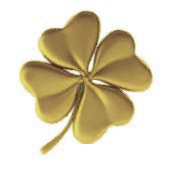
\includegraphics[height=.8em]{clover.png}

\newpage

\section*{Format of the Thesis}
\addcontentsline{toc}{chapter}{Format of the Thesis}

This thesis consists of 6 chapters. Chapter \ref{chap:intro} is an introduction to the different topics relevant to my PhD work and presents its hypotheses and objectives.
Chapter \ref{chap:loy}-\ref{chap:rep} are original research chapters.
Chapter \ref{chap:loy} contains a manuscript that was published in {\it Scientific Reports}\cite{Arseneault2017}.
Chapter \ref{chap:epi} contains a manuscript that was published in {\it PLoS Genetics}\cite{Monlong2018}.
The manuscript in Chapter \ref{chap:rep} was published in {\it Nucleic Acids Research}\cite{Monlong2018nar}.
Chapter \ref{chap:disc} is a general discussion about the benefits of population-based approaches for CNV detection in whole-genome sequencing data.
Chapter \ref{chap:conc} concludes the thesis and describes future directions for population-based approaches of structural variant detection.

\nameref{append:other} lists other publications to which the thesis author have contributed during the thesis period.
\nameref{append:loy}, \nameref{append:epi} and \nameref{append:rep} contain supplementary material for chapters \ref{chap:loy}, \ref{chap:epi} and \ref{chap:rep}, respectively.

\newpage

\section*{Contributions of Authors}
\addcontentsline{toc}{chapter}{Contributions of Authors}
\label{sec:cont}

Chapter \ref{chap:intro} contains a literature review covering sequencing technology, structural variation, genomic repeats, cancer and epilepsy.
Chapter \ref{chap:disc} and \ref{chap:conc} contains a general discussion and future directions about population-based approaches and whole-genome sequencing studies.
These chapters were written by the thesis author under the supervision of Dr. Bourque.

Chapter \ref{chap:loy} represents a manuscript authored by Madeleine Arseneault, Jean Monlong, Naveen S. Vasudev, Ruhina S. Laskar, Maryam Safisamghabadi, Patricia Harnden, Lars Egevad, Nazanin Nourbehesht, Pudchalaluck Panichnantakul, Ivana Holcatova, Antonin Brisuda, Vladimir Janout, Helena Kollarova, Lenka Foretova, Marie Navratilova, Dana Mates, Viorel Jinga, David Zaridze, Anush Mukeria, Pouria Jandaghi, Paul Brennan, Alvis Brazma, Jorg Tost, Ghislaine Scelo, Rosamonde E. Banks, Mark Lathrop, Guillaume Bourque and Yasser Riazalhosseini.
The thesis author developed the computational methods for WGS analysis, analyzed WGS data and generated the figures.
YR conceived the study and designed the experiments with contribution from GB.
NV, PH, LE, IH, AB, VJ, HK, LF, MN, DM, ViJ, DZ, AM, PB, GS and REB were responsible for patient selection, sample collection, sample preparation and pathological reviews.
MA and NN prepared DNA, performed experiments to detect loss of chromosome Y and analyzed the data with contribution from PJ.
PP, RSL, PJ and AlB performed the gene expression analysis.
ML provided critical advice on data analysis and statistical approaches.
MS and PJ performed functional analysis with cell line models.
MA and YR wrote the manuscript, with assistance from JT, GS and REB.

Chapter \ref{chap:epi} contains a manuscript by Jean Monlong, Simon L. Girard, Caroline Meloche, Maxime Cadieux-Dion, Danielle M. Andrade, Ron G. Lafreniere, Micheline Gravel, Dan Spiegelman, Alexandre Dionne-Laporte, Cyrus Boelman, Jacques L. Michaud, Guy Rouleau, Berge A. Minassian, Guillaume Bourque and Patrick Cossette.
The thesis author implemented the method, performed the analysis with SLG, ADL and DS, designed the experimental validation with CM and SLG, and wrote the manuscript with SLG and GB.
SLG, GB and PC conceived and designed the study.
DMA, MG, CB, JLM, GR, BAM, RGL, FH performed the clinical recruitment.
CM and MCD performed the experimental validation.

The manuscript in Chapter \ref{chap:rep} was authored by Jean Monlong, Patrick Cossette, Caroline Meloche, Guy Rouleau, Simon L. Girard and Guillaume Bourque.
The thesis author and GB conceived and designed the study.
The thesis author performed the analysis, designed the experimental validation with CM and SLG, and wrote the manuscript with GB.
PC, GR and SLG provided data and resources for the method validation.
CM performed the experimental validation.

The contribution of the thesis author to other manuscripts is described in \nameref{append:other}.


\chapter{Introduction}
\label{chap:intro}
\fancyhead[RO,LE]{\leftmark}
%% Back to page numbers
\doublespacing
\pagenumbering{arabic}
%% Introducing SV and CNV
\section{Structural Variation and Copy-Number Variation}

\subsection{Types of Structural Variants}
Structural variants (SVs) are defined as genetic variation of more than 50 base pairs.
The different canonical forms of SV include deletion, duplication, novel insertion, inversion and translocation\cite{Hall2012}.
Deletions and duplications of a genomic region, which affect DNA copy number, are collectively known as copy number variants (CNVs).
A duplication can be broadly defined as a gain in copy number of a region, either in tandem configuration (tandem duplication) or in a distant locus.
In contrast, inversion and translocation are considered balanced rearrangements: no DNA sequence is lost or gain.
In reality, small deletion or duplication are often present around their breakpoints\cite{Sudmant2015a,Collins2017}.
\begin{comment}
  In \citet{Sudmant2015a}, only 20\% are simple inversions; 54\% are duplicated inversion and the rest with other CNVs.
\end{comment}
Transposable elements retrotransposition creates mobile element insertion (MEI).
Because these elements are present in the genome, polymorphic MEI are often considered CNVs.
In general, a ``novel'' insertion involves the insertion of a DNA sequence absent from the genome, e.g. viral DNA, but the term is also used in the MEI literature to describe a new insertion of a transposable element.

Complex SVs involve a combination of canonical forms at the variant level\cite{Quinlan2012}.
In a recent study using high-depth long-insert and linked reads sequencing\cite{Collins2017}, thousands of SVs were found to be complex.
\begin{comment}
  In \citet{Collins2017} 2.5\% were complex, 16.8\% were balanced or complex.
\end{comment}
Most of these complex SVs (84.4\%) involved inversions, consistent with previous studies that had noticed small deletions and duplications at inversions breakpoints\cite{Sudmant2015a,Collins2017,Brand2015}.
\begin{comment}
  \citet{Brand2015} describe dupINVdup variants, i.e. paired duplications flanking an inversion. 8.1\% of patients with autism spectrum disorder had one and they found that only 39.3\% of inversions were canonical.
\end{comment}
More extreme genomic events can create complex SVs that combine dozens of canonical forms and span large regions or several chromosomes.
An example is chromothripsis, also called chromosome shattering, which creates a highly fragmented profile with dozens of segments recombined in a different order resulting in a patchwork of duplicated/deleted/inverted regions.
%% Chromoanasynthesis and chromoplexy
While originally though to be rare, recent surveys showed a higher than expected prevalence of somatic and germline chromothripsis.
\begin{comment}
  Using arrays, \citet{Zack2013} estimated that 5\% of the tumors experienced chromothripsis, while \citet{Kim2013b} came up with a lower number of 1-2\%.
\end{comment}
For example, a pan-cancer study found chromothripsis in 38.9\% of the glioblastomas and in 8.7\% of other cancer types\cite{Malhotra2013}.
In the recent study of 689 individuals with autism spectrum disorder and other developmental abnormalities, two cases harbored germline chromothripsis\cite{Collins2017}.

While SVs are intuitively defined in relation to the ancestral state of the genome, it is important to note that in practice the reference genome is used as baseline.
As a result, a variant is a difference in sequence compared to the reference genome but not necessarily compared to the ancestral genome. 
For example, a recent mobile element insertion might be present in the reference genome but when absent, i.e. in the ancestral state, it is often called a deletion.
Similarly, rare deletions of unique regions in the reference genome would resemble novel insertions.

CNVs and in particular deletions have been widely studied.
One reason is technological as large CNVs have been routinely studied before the advent of high-throughput sequencing, for example using karyotyping or hybridization approaches (see section \ref{sec:prehts}).
In addition, CNVs, and in particular deletions, are though to have a stronger functional impact compared to balanced variants.
A deletion disrupts an entire region and potentially several genes while balanced SVs or insertions might affect only the regions around the variant boundaries or insertion site.

The gain or loss of a full chromosome, also called aneuploidy, is particularly rare in normal cells due to the large phenotypic effects of a dosage change in hundreds to thousands of genes.
However, aneuploidy is a hallmark of cancer and observed frequently across cancer types, as described in Section \ref{sec:canceraneu}. 
With whole-genome doubling, full or arm-level chromosomal CNVs are at the high end of the variant size spectrum.

\subsection{Mechanism of Formation}
The mechanisms of SV formation are diverse and result in a heterogeneous distribution of SV across the genome, both in term of size and location\cite{Hall2012,Sharp2006,Mills2011}.
New variants can occur during DNA repair, recombination, replication or through retrotransposition.

Non-homologous end joining (NHEJ) is a DNA repair mechanism that often results in deletions.
In the presence of double-strand breaks, the two ends slowly denature until the arrival of the repair machinery that joins the two ends.
Occasionally, misalignment of the overhanging ends lead to small insertions.
Larger sequences can also be incorporated during the repair, leading to large insertions.

Microhomology-mediated end joining (MMEJ) is a type NHEJ which repair the double-strand DNA breaks using micro-homology (5-25 bp) between the broken ends. 
MMEJ often result in deletions of the sequence between the micro-homology regions but can also create translocation and more complex variants.

Homologous recombination is another repair mechanism that uses a template, usually another chromatid, to repair double strand breaks.
By aligning a template, homologous recombination can repair accurately a double strand break even if part of the original nucleotides were lost.
Mis-alignment, potentially due to the presence of repeats, results in repair between non-allelic regions and leads to deletions.

Similarly, non-allelic homologous recombination (NAHR) occurs when sister chromatids are not correctly aligned during recombination.
Depending on the mis-alignment configuration, NAHR results in deletion, duplication or inversion.
%% Potentially more on the different configuration and resulting SV types.
The chromatid misalignment is often caused by the presence of highly similar sequences.
Genomic repeats like segmental duplications and transposable elements are frequent templates for NAHR.
The majority of NAHR in recent human evolution involved L1 elements although Alus are enriched around older rearrangements\cite{Bourque2009,Kim2008}.
NAHR can also occur during mitosis\cite{Gu2008}.


Fork stalling and template switching (FoSTeS) occurs during DNA replication when a strand is detached from its current fork and continues replicating in another strand.
Depending on the sequence of switches, FoSTeS can result in a translocation, deletion, duplication or inversion.

Slippage during DNA replication can lead to small deletions or duplications, creating and maintaining tandem repeats.
Short tandem repeats are particularly susceptible to shrinkage or expansion using this mechanism.
While each slippage might only affect a few base pairs, sequential events lead to polymorphic alleles that can differ by hundreds of base pairs between two genomes.
\begin{comment}
  Slippage occurs when the DNA polymerase and the newly synthesized stand detaches when it encounters a DNA repeat and reattach after pairing with a non-allelic repeat, usually upstream (resulting in expansion).
  The shrinkage/expansion is caused by the template/daughter strand contracting when forming a hairpin due to the repeats.
  This type of repeat-induced secondary structure can also contribute to the replication stalling and detachment.
\end{comment}

To retrotranspose, a mobile element is first transcribed into a RNA copy which is then converted back to a DNA.
The DNA copy then inserts itself at another location of the genome.
The DNA sequence of autonomous TEs, such as L1s, code for proteins responsible for the reverse transcription and insertion into the genome.
Other TEs use the machinery from autonomous elements to retrotranspose. 
A similar mechanism is responsible for the insertion and retrotransposition of viral DNA.
Once inserted in the host genome, the viral DNA can often copy itself in other genomic locations or in other cells.
Similar to retrotransposons, new insertions can then be considered as duplication events.

The mechanism of formation is often inferred from the sequence around the variant boundaries\cite{Mills2011}.
Segmental duplication or large repeats flanking a variant suggest NAHR.
Micro-homology at the boundaries is a sign of MMEJ.
No homology points at either NHEJ or FoSTeS.

Aneuploidy arise from problems with the chromosome migration during mitosis.
The main mechanism behind arm-level losses or gains are fusion of chromosomes after pericentromeric breakage.
Breaks near centromeres can happen in fragile sites, which tend to break under certain conditions, or due to merotelic attachment, an abnormal attachment of sister chromatids during mitosis\cite{Martinez-A2011}.

\subsection{Association with Disease and Functional Impact of CNV}

\paragraph{CNV and disease}

Individuals suffering from numerous diseases including obesity\cite{Bochukova2010}, schizophrenia\cite{Stone2008}, autism\cite{Stefansson2014}, epilepsy\cite{Mefford2011}, Crohn's Disease\cite{McCarroll2008a}, cancer\cite{Beroukhim2010} and other inherited diseases \cite{Balzola2010,Ayarpadikannan2014}, carry SVs with a demonstrated detrimental effect\cite{Conrad2010,Firth2009,Spielmann2013}.
%% DiGeorge/velocardiofacial syndrom is characterized by deletion of 22q11.2.
First, a few Mendelian disorders are exclusively caused by CNV in specific regions.
For example, Williams-Beuren Syndrome which typically presents facial dysmorphies and intellectual disability, is caused by deletions at 7q11.23.
As another example, the deletion of the {\it PMP22} gene is the most common mutation responsible for hereditary neuropathy with liability to pressure palsies.
\begin{comment}
  {\it PMP22} protein is a component of myelin, a substance that protects nerves, and seem to be specifically responsible to protecting nerves from physical pressure.
\end{comment}
In the early 1990s, Lupski et al. were surprised to find that a duplication in the same region segregated perfectly with hereditary neuropathy Charcot-Marie-Tooth type 1A\cite{Lupski1991}.
The region had been identified using linkage analysis but the idea of a gene-dosage mechanism for the disease was so unexpected that both {\it Nature} and {\it Science} refused to review the paper.

CNVs resulting in gene-dosage changes have often milder effects but many have been associated with complex traits or susceptibility to disease.
Frequent deletions in the {\it GSTM1} gene were identified as a risk factor for asthma in independent studies across different populations\cite{Liang2013}.
Another example of common disease-associated CNV involve the {\it DEFB4} gene.
The median copy number of this gene is 4 in healthy individuals.
A lower number of copies has been associated with Crohn disease\cite{Fellermann2006} and higher copy number with psoriasis\cite{Hollox2008}.
\begin{comment}
  \citet{Fellermann2006} found a significantly lower copy number in this gene in a cohort of colonic Crohn's Disease and another of inflammatory bowel disease.
  Individuals with 3 copies or fewer were three times more likely to develop colonic Crohn's Disease than individuals with 4 copies or more.
  \citet{Hollox2008} observed a higher copy number in psoriasis patients in two cohorts of Dutch and German individuals.
\end{comment}
Deletions and duplications of the {\it CCL3L1} gene are also associated with distinct phenotypes.
Deletions increase HIV/AIDS susceptibility\cite{Gonzalez2005} while duplications increase the risk to develop rheumatoid arthritis\cite{McKinney2008}.
\begin{comment}
  {\it CCL3L1} is located in a segmental duplication and encodes a cytokine protein.
  The CNV status was tested with RT-PCR on 1K controls from 57 populations and 4K HIV+ and HIV- individuals.
  The same approach was performed for rheumatoid arthritis on 1K cases from NZ and UK and 1.5K controls.
\end{comment}
In the examples above, variation in the copy number of the entire gene is affecting the gene dosage resulting in gene expression changes.
Although genes with common CNVs are assumed to be tolerant to dosage changes, gene expression tend to change with the number of gene copies in the genome.
For example, \citet{Handsaker2015} studied multi-copies CNVs and showed that the resulting gene dosage changes correlated with gene expression.

\paragraph{CNV and gene expression}

Quantitative trait loci (QTL) and more precisely expression QTLs (eQTLs) are genomic variants that are associated with changes in gene expression.
While most of the eQTLs tested and found are single nucleotide variants (SNVs), WGS has allowed the detection of hundreds of SV-eQTLs.
Among the first to look for SV-eQTLs, Stranger et al. identified dozens of CNVs in four human populations that were associated with gene expression\cite{Stranger2007b}.
Around half of the associated CNVs were located outside of the affected gene or only overlapped partially, hinting at an alternative to the gene dosage mechanism.
Later, Lower et al. characterized deletions that affected the expression of a gene located 300 Kbp away, {\it NMEA}, by analyzing gene expression and using conformation capture to demonstrate physical contact between the two distant regions\cite{Lower2009}.
Combining their WGS data with RNA sequencing across 462 individuals, the most recent SV catalog from the 1000 Genomes Project identified 54 eQTLs whose lead variant was a SV and 166 additional SVs that were in linkage disequilibrium with SNV-eQTLs\cite{Sudmant2015a}.
Most of these SV-eQTLs overlapped coding sequence but some were located in non-coding regions upstream of the affected gene.
Only 0.56\% of the eQTLs were attributed to SV but this number might be an underestimation because of the higher noise in SV calling compared to SNV calling.
To improve on this, a recent study used deep WGS to more reliably call SVs and investigated SV-eQTLs in multiple tissues from the GTEx dataset\cite{Chiang2017}.
Using state-of-the-art approaches to infer causal variants, they estimated that 3.5-6.8\% of eQTLs could be attributed to SVs.
Although less abundant than SNV-eQTLs, SVs had a larger effect size.
The comprehensive analysis of the location and effect of these causal SV-eQTLs nicely clarified the relation between SV and gene expression.
When overlapping coding regions, SV-eQTLs affected gene expression following the gene dosage model, that is deletion leading to down-regulation and duplication to up-regulation.
Non-coding SV-eQTLs, which represented the vast majority of SV-eQTLs (89\%), were enriched in or close to regulatory regions (e.g. exons, transcription start site, transcription factor binding sites, enhancers, gene 3’ end) and all types of SV could lead to both higher or lower gene expression.
Finally, the effect of rare SVs on gene expression was also explored.
Despite the challenge of analyzing rare variants in a cohort of only 147 individuals, a clear enrichment of rare SVs was found around genes that showed outlier expressions in the cohort.
These gene-altering rare SVs included cases from both the gene dosage and regulatory region disruption model.

%% Enhancer hijacking
Several recent studies elegantly shed light into a mechanism by which non-coding CNV alter gene expression called enhancer hijacking: that is, a regulatory region inducing the ectopic expression of a gene it normally doesn't regulate because of a CNV-mediated re-positioning.
A first example was comprehensively described in individuals with limb malformation\cite{Lupianez2015}.
Using conformation capture sequencing and by recreating SVs in mice with CRISPR/Cas genome editing, they elegantly showed that SVs crossing the boundaries of topologically associating domains (TADs) could lead to strong phenotypes.
TADs are 3D domains (mean size 830 Kbp) that confine regulatory elements with their targets.
The deletions, tandem duplications and inversions resulted in ectopic interactions between a cluster of enhancers and genes located in the neighboring TAD.
Ectopic interactions were responsible for ectopic expression of these genes during limb development in mice whose genome had been edited to recreate the SVs.
With additional genome editing and conformation capture experiments, this study concluded that the crossing of the TAD boundary was the crucial factor rather than simply the distance between enhancers and genes.
Enhancer hijacking might also be important in cancer where a single CNV might lead to a strong expression of oncogenes.
To explore this, \citet{Weischenfeldt2016} developed a method that detects associations between somatic CNV breakpoints overlapping several TADs and gene over-expression.
In their study, \citet{Weischenfeldt2016} first described a known cancer gene, {\it TERT}, which had been already found to be upregulated by such mechanisms.
Interestingly, both deletion and duplication resulted in over-expression.
They further described two genes, {\it IRS4} and {\it IGF2}, using orthogonal experiments to support how the presence of somatic CNVs lead to changes in chromatin state and physical contact.
For example, somatic deletions downstream of {\it IRS4} overlapped a TAD boundary and resulted in 25-400 fold over-expression of the gene in several cancer types.
In contrast, the ectopic expression of {\it IGF2} was due to single tandem duplication of {\it IGF2} and a super-enhancer in the neighboring TAD that created a novel chromatin domain with both.
Additional experiments showed that the region was active and in contact with the gene promoter in tumor with the duplication.
These enhancer hijacking events are important because the change of a single copy can lead to large over-expression.
In contrast, dosage effect due to full-gene CNV tend to be as strong as the amplification.

\section{Whole-Genome Sequencing}

\subsection{SV Detection Before High-Throughput Sequencing}
\label{sec:prehts}

Early cytogenetic techniques were able to detect aneuploidy and extremely large SVs.
Thanks to banding, each chromosome in a karyotype can be uniquely identified which facilitated the detection of trisomies and their associated disorder, such as Down syndrome (trisomy 21) and Edwards syndrome (trisomy 18).
Furthermore, the bands can be used to identify translocations and large inversions or CNVs.
SVs need to span several millions of bases, typically more than 10-20 Mbp, to have a chance to be visible in the karyotype.

Fluorescent {\it in situ} hybridization (FISH) was developed in the 1980s.
Fluorescent probes bind to specific genomic regions by hybridization, i.e. through DNA sequence complementarity.
The presence or absence of the DNA sequence was assessed by inspecting the fluorescence in the cells or tissue samples.

In array comparative genomic hybridization (aCGH) experiments, DNA from a test sample and reference sample are labeled using different fluorophores and hybridized to several thousand probes.
The probes, which usually tag most of the known genes and tile non-coding regions of the genome, are printed on a glass slide.
The fluorescence of each probes is used to estimate the amount of DNA sequence in the test sample compared to the reference sample.
Using this method, CNV down to approximately 100 Kbp of DNA sequences can be detected.
Arrays also can be designed specifically to target regions of interest, for example with recurrent CNVs.
These custom arrays don't cover the genome uniformly but can detect smaller CNVs in the regions with of high probe density.
This technology is not able to detect balanced chromosomal imbalances such as translocations or inversions.

%% Amplification and Sanger sequencing

\subsection{A New Hope}
While large SVs have been identified by cytogenetic approaches and array-based technologies, whole-genome sequencing (WGS) could in theory discover SVs of all sizes or types\cite{Alkan2011}.
The vast majority of studies follow a re-sequencing strategy where short DNA fragments (or reads) are sequenced and aligned (or mapped) to the reference genome.
Furthermore, both ends of a DNA fragment are often sequenced and this pair information can be used to improve alignment to the reference genome and variant calling.
The reads and their alignment are then used to find single-nucleotide variants (SNVs), small insertions/deletions (indels) but also small SVs across the genome.
Array-technology required dense representation of the hybridization probes in a region of interest to be able to detect CNVs smaller than 100 Kbp.
With WGS, the sequencing depth is now the main limiting factor, although even early experiments could detect thousands of small SVs.
For example, the most recent survey of the 1000 Genomes Project used WGS with a sequencing depth of 7x and identified more than four thousands variants per individual with a median variant size below 40 Kbp for the six different SV types analyzed\cite{Sudmant2015a}.
In contrast to aCGH, the sequencing reads can also be used to detect balanced variants such as inversions, translocations and novel insertions.
Although the detection of such variants is more challenging than single-nucleotide variant (SNV) calling, WGS is a one-fit-all experiment that greatly increases the resolution of SV detection.

To detect SVs from WGS, methods analyze either read-depth (RD) variation\cite{Boeva2011,Abyzov2011,Klambauer2012}, paired-end information\cite{Chen2009,Lindberg2014}, breakpoints detection through split-read approach\cite{Ye2009} or {\it de novo} assembly\cite{Rimmer2014}.
Methods are described in more details in section \ref{intro:methods}, with a particular focus on CNV detection.

Another unique aspect of WGS is the possibility of pooling experiments to increase the detection power of common variants.
Instead of analyzing each experiment separately, the sequencing reads can be pooled across several samples.
For example, it is sometimes challenging finding several reads spanning a SV breakpoint within a single sample.
By pooling several experiments, the number of supporting reads increases if a SV is shared by several samples.
This approach was used across hundreds of samples of the 1000 Genomes Projects and greatly increased the number of SVs discovered in the population\cite{Mills2011,Handsaker2011}.

\subsection{The Technical Bias Strikes Back}
Although it represents a considerable improvement in term of resolution, WGS is affected by technical biases that remain an important challenge.
Indeed, it has been shown that various features of sequencing experiments, such as mappability, GC content or replication timing, have a negative impact on the uniformity of the coverage\cite{Treangen2011,Teo2012,Benjamini2012,Koren2014,Cheung2011}.
In addition to its effect on read coverage, repeated sequences lead to confusion in read mapping, creating SV-like patterns and thus false-positives when calling variants.

GC content is a well-known source of bias although not completely understood.
Reduced efficiency of PCR amplification explains a large fraction of this bias and more robust protocol were proposed\cite{Aird2011,Kozarewa2009}.
\begin{comment}
  \citet{Aird2011} improved PCR protocol by using longer denaturation steps, different temperature for primer annealing, different reagents/polymerase.
  \citet{Kozarewa2009} introduced a PCR-free protocols where the amplification is performed after cluster formation rather than before (I think).
\end{comment}
Still other steps of the sequencing protocols adds substantial bias and GC bias persists even with optimized protocols\cite{Aird2011}.
The bias patterns tend to be different from a sequencing center to the other\cite{Benjamini2012}, suggesting an effect of the library preparation or sequencing machinery.
For these reasons, it has been challenging to correct for this source of bias.
With PCR-free libraries, the effect of GC bias is reduced but still needs to be corrected for when comparing read coverage across the genome.

DNA replication also affects the distribution of reads across the genome.
Although sequencing of bulk samples, i.e. of many cells, should minimize the effect of replication patterns, systematic increase might be present in regions that tend to replicate earlier.
For example, Koren et al. estimated replication timing across the genome using WGS of cells in S and G1 phases\cite{Koren2012}.

Finally, the mappability of the sequence affects how many reads can be confidently mapped to the reference genome.
The presence of repeats and other similar regions lead to multi-mapping, i.e. several positions where a read could have originated from.
Hence, when using reads with unique mapping in the genome, the coverage in repeat-rich regions drops considerably.
The challenges and proposed solutions associated with mappability are described in more detail in section \ref{intro:map}.

Unfortunately, the variability in term of read distribution is difficult to model and correct for because it involves various factors, including some that vary from an experiment to another and others that are still unknown.
This issue particularly impairs the detection of SV supported by weaker signal, which is inevitable in regions of low-mappability, for smaller SVs or in cancer samples with stromal contamination or cell heterogeneity.

\subsection{The Return of the Long Reads}
Sanger sequencing, invented in 1977\cite{Sanger1977}, was used for the original sequencing of the human genome\cite{Lander2001} and is still used today to sequence DNA fragment 500 to 1000 bp long.
The technology that followed in the 2000s is capable of sequencing shorter reads but much more efficiently resulting in a cost order of magnitudes lower.
However, many of the challenges faced by WGS is a result of the short size of the sequenced read.
Recently, new technologies have been developed to perform WGS using much longer reads, in the range of 10-100 Kbp.
PacBio was the first and has been successfully applied to several human genomes\cite{Chaisson2014,Pendleton2015,Huddleston2016}.
Nanopore sequencing is becoming efficient with the first human WGS sample just released publicly\cite{Jain2018}.
Although the cost and rate of sequencing errors remains high compared to short-read sequencing, the benefit for genome assembly or SV detection is clear.


\section{Existing CNV Detection Methods}
\label{intro:methods}

\subsection{Different Strategies to Detect SV and CNV}

The vast majority of SV detection methods rely on evidence from the read mapping on a reference genome: changes in read depth, B-allele frequency, discordant paired-end mapping, or split-reads.
{\it De novo} genome assembly could also be used to identify SVs but its application using short read sequencing remains challenging.

\paragraph{Read depth}
Changes in the copy number in a region should lead to changes in the number of reads mapped to this region in the reference genome.
By modeling read depth, sometimes called read coverage or depth of coverage, one approach is to identify regions with significantly more reads (duplication) or fewer reads (deletion) than in the genome or the flanking regions.
Only CNV, i.e. imbalanced SVs, can be detected by these approaches.
CNV detection methods that use read depth are described in more details in the next section.
% Resolution: the larger the variant the better. The more sequencing the better

\paragraph{B-allele frequency}
The proportion of reads supporting heterozygous SNVs can help identify CNVs too.
The loss of heterozygozity within deletions or the deviation from the 50\% coverage of the alternate allele can complement coverage signal.
This approach was inspired from CNV detection strategies developed for SNP-array, such as in the {\sf ASCAT} method\cite{VanLoo2010}.
Here the intensity of the probe and the so-called B-allele frequency was use in concert to call CNVs.
Thanks to sequencing, both the coverage information and SNVs are more densely represented and lead to a better resolution.
Still, the B-allele information is relevant only for CNVs large enough to span several heterozygous SNVs.
Methods such as {\sf ERDS}\cite{Zhu2012}, \textsf{Control-FREEC}\cite{Boeva2012} or \textsf{Sequenza}\cite{Favero2015} integrate the B-allele frequency information to call germline or somatic CNVs.
% Resolution: the larger the variant the better. The more sequencing the better but not as much.

\paragraph{Paired-end mapping}
The distance between the two mapped reads in a pair and their orientation can also help identify SVs.
Because the majority of the reads are expected to map correctly, they can be used to estimate the expected distribution of the distance between paired read.
With this distribution, one strategy is to retrieve pairs that are significantly too close or too far from each other.
Read pairs might map close to each other in the reference genome because of an insertion in the sequenced DNA somewhere between the reads.
More typically, reads that map far from each other suggest a deletion in the sequenced DNA or potentially a translocation.
Finally, tandem duplications or inversions should lead to some read pairs mapping in the incorrect orientation relative to each other.
All those reads with discordant paired-end mapping are typically retrieved and clustered together.
Each cluster of reads is then disentangled to predict the most likely variant and the location of its breakpoints.
% Resolution: The more sequencing the better

\paragraph{Split-reads}
The strategies described above use either reads within the variant or around the variant's boundaries.
In contrast, the split-read approach looks for reads exactly spanning a variant's breakpoint.
%% Although it can be used with single read sequencing, paired-sequencing improves its accuracy drastically.
Generally, one read is mapped uniquely to the genome and serves as an anchor while its pair is split in two pieces which are then aligned separately.
This split-mapping can be computationally expensive.
To limit the computational cost, methods analyze only pairs with one unmapped reads or restrict the range searched for the split-mapping\cite{Ye2009,Faust2012}.
Split-reads can be searched specifically to complement candidates variants identified from discordant paired-end mapping.
These additional supporting reads are tallied and used to assess the final supporting evidence in methods such as \textsf{LUMPY}\cite{Layer2012} or \textsf{DELLY}\cite{Rausch2012}.
% Resolution: The more sequencing the better. The smaller the better sometimes.

\paragraph{Assembly}
Local assembly of reads around candidate variants has been used as in silico validation and to characterize the breakpoint sequence\cite{Wong2010,Chen2014}.
Going further, recent methods have been using local read assembly as their main SV detection strategy, especially in cancer\cite{Zhuang2015,Chong2016}.
If {\it {\it de novo}} assembly keeps improving, for example thanks to longer reads, SV could also be called by directly comparing assembled genomes or to the reference genome.
For example, \textsf{Assemblytics} has been recently developed to align two assembled genomes and to annotate SVs that differentiate them\cite{Nattestad2016}.

\subsection{CNV Detection Using Read Depth}

\paragraph{Single-sample methods}
The first methods that used read-depth signal to call CNVs assumed a uniform read coverage across the genome and attempted to segment it along the chromosomes.
The segments produced by these approaches represent regions with similar copy number.
The circular binary segmentation, adapted from aCGH analysis\cite{cam2008ide}, was one of the first and remains a popular segmentation algorithm.

Subsequent methods offered better correction of technical biases and more modern segmentation techniques.
For example, {\sf CNVnator}\cite{Abyzov2011} corrects for the GC bias, masks repeat-rich content and uses a mean-shift segmentation approach inspired from the image recognition field.
{\sf CNVnator} has been used extensively in both germline and somatic CNV surveys\cite{Sudmant2015a,Chiang2017}.
{\sf FREEC}\cite{Boeva2011} is another popular approach that can correct for both GC bias and mappability using precomputed tracks.
It segments the corrected read-depth signal with a LASSO-based segmentation approach.
{\sf FREEC} has been extended to {\sf Control-FREEC} to include the B-allele frequency in its CNV detection process.

Methods inspired from aCGH offer to use another sample as control.
Although variants in the control sample might create problems down the line, it is particularly sensible when studying tumors whose tumoral and normal tissues has been sequenced.
By using the normal sample (usually blood) as control, the CNV detection is naturally reduced to the detection of somatic CNVs, i.e. present in the tumor but absent from the normal sample.
In practice the methodology is similar to the single-sample approaches described above but using the read-depth ratio of the tumor versus normal tissues.
A few methods have further been implemented specifically with cancer in mind and estimate the tumor ploidy and/or stromal contamination before or during CNV calling\cite{Favero2015,Ha2014}.

\paragraph{Multi-samples methods}
% Strength in numbers
To improve the sensitivity of the variant detection and model the region-specific pattern of read depth, a few methods have been developed to jointly analyze multiple samples together.

{\sf cn.MOPS} considers simultaneously several samples and detects copy number variation using a Poisson model and a Bayesian approach\cite{Klambauer2012}.
By jointly analyzing samples, {\sf cn.MOPS} calls variants based on the strength of the read-depth signal across the samples.
Even if the signal-to-noise ratio is small, the presence of a consistent pattern in several samples provides further evidence that the region contains a CNV in those samples.

The second version of {\sf GenomeSTRiP} models the read depth across hundreds of samples as a mixture of Gaussian distributions\cite{Handsaker2015}.
It is particularly useful to genotype multi-copies variants in the genomes, i.e. regions that have more than two copies in most individuals.
Multi-copies variants create different groups of samples that translate into different RD distributions.
By deconvoluting the mixture of distributions, the relative difference between RD modes help associate each distribution (and sample) to a copy-number estimate.
As it relies on full signal (i.e. around integer values in the model) and a simple read-depth normalization, it is still limited in regions with low coverage and for small or rare variants.
The power to detect a variant increases with the frequency of polymorphisms as more individuals populate the different genotype groups, improving the copy-number estimation.
{\sf GenomeSTRiP 2.0} was successfully applied to 849 individuals from the 1000 Genomes Project and unmasked the population variation of hundreds of multi-copies variants.

Both {\sf cn.MOPS} and {\sf GenomeSTRiP} use the additional samples to find further support for a variant, which is particularly efficient at detecting common CNVs.
However, both methods define models with full copy number changes which has limited power when dealing with CNVs with partial signal (e.g. small variants, somatic variants, or variants in low-mappability regions).
In contrast, the approach described later in this work uses the multiple samples differently: they are used to define a baseline for the technical variation, not to aggregate evidence supporting a variant.
When the coverage diverges enough from this baseline, no matter the frequency or the strength, a CNV is called.
In theory such approach will be able to better detect rare variants, small variants, somatic variants and variants in low-mappability regions.

These approaches are also called population-based methods because they jointly study a population sample of sequencing experiments, i.e. a group of samples representative of the technical variation across experiments\cite{Handsaker2015}.
Of note, the term population in this context refers to a statistical population rather than human populations.

\section{Low-Mappability Regions} 
\label{intro:map}

\subsection{The Different Classes of Human Repeats}

1.53 Gbp of the human genome is annotated as a repeat when considering elements identified by Repeat Masker\cite{Smit2015} and segmental duplications.
Repeats are classified based on their size, sequence and mechanism of formation.

Segmental duplications (SDs) are large regions ($>$1 Kbp) with high similarity ($>$90\%).
Usually the results of NAHR, segmental duplication are known hotspots of structural variation.
SDs can be nested, i.e. duplications within duplications.
These class of repeat is thought to have boosted recent human evolution\cite{Bailey2006}.
Humans experienced a high rate of SD creation in recent evolution which contributed to the expansion of important gene families.
Large families of genes involved in immune response, cell adhesion and brain development cluster within SDs.

Transposable elements (TE) represents approximately 45\% of the human genome.
TEs are interspersed in the genome: if we cut the reference genome in consecutive windows of 500 bp, 70.5\% of the windows would overlap transposable elements.
Their wide distribution make them a popular template for NAHR.
Some TE families tend to cluster in fragile regions of the genome, which are regions that tend to break under certain stress conditions.
A small fraction of TEs of the Alu, L1 and SVA families are still active in the human genome\cite{Mills2007}.
Retrotransposition of these elements contributes to novel MEI.

Satellites consist of sequences that are repeated, most of the time in a tandem configuration, and span large regions.
The size and composition of the repeated sequence, also called unit, define the different classes of satellites.
Most of the macro-satellites are present close to centromeres, the main family being alpha satellites whose 171 bp long unit is repeated to span on average 5.6 Kbp.
The sequence of the unit varies from chromosome to chromosome.
In addition to the tandem repetition of the unit sequence, higher order structure is present.
The sequences can be duplicated in the same orientation or in an inverted conformation.

Short tandem repeats (STRs), also called micro-satellites, have sequence units ranging from 1 to 10 bp.
In addition to the tandem duplication that they share with SDs and satellites, short tandem repeats can vary because of slippage during the replication process.
As a result, STRs are one of the most polymorphic class of variant in the human population, making them particularly useful for forensics and parentage tests.
STRs have been recently linked to gene expression regulation\cite{Gymrek2016,Quilez2016} and potentially to polygenic disorders\cite{Hannan2018}.

Low complexity regions are regions with high AT or GC content that, unlike satellites, have no apparent structure.
Very little is known about their mechanism of formation and variation.
Longer stretches of similar sequences might be present by chance in those regions which might promote homology-based mechanisms of CNV.
Low complexity sequences might also favor secondary DNA structure, promoting replication slippage.

\subsection{Impact of Repeats on Mappability}
The presence of repeats can confuse read mapping and decrease the number of uniquely mapped reads in certain regions.
These low-mappability regions can contain any class of repeats, e.g. segmental duplication, transposable elements, short tandem repeats or low-complexity sequences.
The effect of repeats on the mapping of a read is specific to each region: it depends on the density and nature of the repeats present. 
As a result, this technical variation is difficult to model.
Existing methods either remove the signal in these regions or smooth the signal to avoid spurious variation (see \nameref{sec:repmeth}). 

Furthermore, the multi-mapping of reads between similar repeat instances resembles signal supporting certain SVs.
For instance, translocation are supported by pairs of reads mapped far from each other.
When one read of the pair spans a repeat, it is sometimes aligned to another repeat element in the genome, far from its paired read.
To minimize this issue, read aligners could favor configurations where both pairs map together but forcing read pairs to map together would impair the detection of real variants.
In practice, some aligners output the best alignment as well as other secondary alignments where the reads could have originated from.
This multi-mapping information or other mapping metrics are used by SV callers to identify legitimate variants or flag others that could be caused by mapping confusion.
Nonetheless, even with paired-end aware mappers many reads overlapping repeats show this incorrect mapping and can hinder SV calling.
Because a low-mappability sequence highly resembles another sequence in the genome, a variant or a sequencing error in the read might lead to a better (although incorrect) mapping in the incorrect location.
This multi-mapping confusion can also occur locally and incorrectly support other types of SVs such as deletion and tandem duplications.

To minimize the effect of multi-mapping, algorithms tend to use uniquely mapped reads only.
Fewer reads support the presence of a variant but they are of better quality.
In some cases, repeats flank a unique region and can mask potential CNVs from paired-end or split-read approaches that use uniquely mapped reads only.
Indeed, because of the repeats, reads around the breakpoints that would support the CNV don't map uniquely. 
If the flanking repeats are long and highly similar, these CNVs can only be detected by changes in the read coverage.

\subsection{Tackling the Repeat Challenge}
\label{sec:repmeth}

Because of the mappability and other technical biases, existing approaches suffer from limited specificity and sensitivity\cite{Mills2011,Alkan2011}, especially in specific regions of the genome, including regions of low-complexity and low-mappability\cite{Treangen2011,Teo2012}.

Approaches that use paired-read information and split-read mapping are difficult to modify to deal with the presence of repeats.
Oftentimes, repeated regions or low-confidence mapping are simply filtered (or flagged) when calling SVs.
The integration of the multi-mapping information could always be improved but the mapping patterns are often region-specific and difficult to model.
Despite the challenges, some attempts were made for specific types of variants.
For example, \citet{Hormozdiari2010} modeled transposon insertion and \citet{He2011} proposed a way to handle the multi-mapped reads when searching for tandem duplication.

Approaches relying on read coverage are relatively more robust because they use signal across the whole variant rather than the breakpoint regions.
A deletion or duplication between repeated sequences might be difficult to call confidently using paired-end or split-read information but the change in RD across a variant is less affected by repeats around the breakpoints.
The presence of repeats along the entire variant still remains a challenge for RD approaches.
To deal with regions of high repeat content, repeats were originally masked before CNV detection to avoid problems from multi-mapping of the sequencing reads\cite{Alkan2009,Sudmant2010a}.
Another approach used bins of variable length designed specifically to provide uniform coverage of uniquely mapped reads across the genome\cite{cam2008ide}.
For example, a region with repeats was extended as much as necessary to contain, on average, a similar read coverage as in unique regions.
While it simplified the methodology of the CNV calling, it was not ideal.
First, repeat-rich regions often remained problematic and were still specifically filtered out of the output.
Indeed, repeat-rich regions are not only less covered by uniquely-mapped reads but also more variable.
The variable-length bin design adjusted the mean read coverage but the repeat-rich regions remained more variable and challenging for most segmentation approaches.
Second, the contribution of the repeat-rich regions in the extended bin becomes minimal because of their low coverage.
The repeats are not masked but they are not represented by the RD of these regions either.
Although it helps mitigate the effect of repeats, it doesn't help address variation in repeat-rich regions.

Other methods keeps repeats unmasked and use bins of equal size but transform the coverage signal to reduce the unwanted effect in repeat-rich regions.
For example, {\sf CNAseg}\cite{Ivakhno2010} and {\sf CNVnator}\cite{Abyzov2011} use a smoothing step that reduce the effect of outliers and smooth the signal using flanking regions.
Similar to the variable-length bin strategy, the signal in the repeat regions is traded off for a easier calling and segmentation.
After smoothing, CNVs in repeat-rich regions but also small CNVs might become invisible.

In an attempt to tackle the problem at its roots, Alkan et al. developed a read aligner to better deal with reads mapping to several locations in the genome\cite{Alkan2009}.
Using {\sf mrFAST} they were able to better detect and genotype copy-number variants in some large and highly similar segmental duplication.
They showed that alignment could be improved for many segmental duplications regions to the point where accurate CNV detection was possible.
However, this effort cannot be replicated for the vast majority of the repeat-rich regions of the human genome.
Alignment algorithms performance in low-mappability regions are now mainly limited by the size of the sequencing reads.


\subsection{Disease-Associated CNV in Repeats}

CAG repeat expansion in a coding region of the {\it HTT} gene causes Huntington disease in a dominant and fully penetrant manner\cite{MacDonald1993,Andrew1993}.
When the short tandem repeat is large enough, typically larger than 36 units, the mutant protein is responsible for an increase in the decay rate of neurons.
Fragile X syndrome is caused by the expansion of a CGG repeat in the 5' untranslated region of the {\it FMR1} gene\cite{Verkerk1991}.
\begin{comment}
  Fragile X syndrome causes Mental Retardation.
\end{comment}
The length of the repeat varies from 15 to 60bp (20 units) in the healthy population while repeats larger than 600 bp cause the disease.
Repeats with intermediate size increase the disease risk for the offsprings.
ICF syndrome (Immunodeficiency, Centromeric instability and Facial anomalies) is characterized by an extension of pericentromeric satellites.
\begin{comment}
  Hypomethylation of these satellites is thought to be the cause for this instability on chromosome 1, 9 and 16\cite{Jeanpierre1993}.
\end{comment}
Facioscapulohumeral muscular dystrophy was associated to the contraction of a satellite DNA in the sub-telomeric region of chromosome 4\cite{Rich2014}.
\begin{comment}
  Healthy individuals have 11-150 units while disease have 1-10 (no repeat doesn't cause the disease).
  D4Z4 repeats is 3303 bp long and contains an ORF (1173 bp) with 2 homeobox domains.
\end{comment}

CNVs involving repeats are also widespread in cancers.
L1 retrotransposition is a common phenomenon in some cancer types such as epithelial tumors\cite{Lee2012b,Tubio2014,Burns2017}.
The first instance of disruptive insertion was documented in the tumor suppressor gene {\it APC} in colon cancer\cite{Miki1992}.
Microsatellite instability is important in some cancers, such as colorectal and endometrial cancers, and usually coincides with the disruption of DNA repair mechanisms\cite{Kim2013}.
It results in extensive copy number changes in microsatellites.
In colorectal cancers, micro-satellite instability is typical of a specific sub-group, Lynch syndrome, representing around 15\% of cases and associated with better prognosis\cite{DelaChapelle2010}.
Fragile sites are also enriched in somatic SVs.
Furthermore, fragile sites are often unstable in cancer and are enriched in low-complexity sequences and satellites\cite{Fungtammasan2012,Durkin2007}.
Transposable elements tend to cluster in these regions as well, sometimes taking advantage of the DNA breaks to insert new copies.
Satellite instability and increased retrotransposition suggest that repeated region might be more fragile or more variable than in normal genomes.

In addition to variation in the repeat sequence, some repeated regions favor the formation of CNVs.
For instance, segmental duplications and TEs provide templates for NAHR.
Alu or L1 elements are the most abundant and most frequent templates.
Alu-mediated deletions in the {\it LDLR} gene were among the first to be described in a patient with familial hypercholesterolemia\cite{Lehrman1985}.
A recombination event between HERV-I copies has been linked to male infertility by causing a $\sim$800 Kbp deletions containing the azoospermia factor gene on chromosome Y\cite{Sun2000}.
\begin{comment}
  \citet{Sanchez-Valle2010} describe another example of HERV-mediated deletion associated with a disease, namely branchio-oto-renal syndrome caused by deletions in the eye absent homologue 1 gene ({\it EYA1}).
\end{comment}
Cancer genes such as {\it MLL-1}, {\it VHL} and {\it BRCA1} seem to be experiencing CNVs resulting from NAHR between Alu elements\cite{Belancio2009}.
\begin{comment}
  For example, Alu-mediated NAHR often creates tandem duplication of the {\it MLL} gene in acute myeloid leukemia.
\end{comment}
Alu-mediated recombinations around {\it MSH2} are responsible for germline deletions that have been linked to susceptibility to hereditary nonpolyposis colon cancer\cite{Li2006}.
CNV can be a byproduct of TE insertion as well. 
For example, the insertion of a L1 lead to a 46 Kbp long pathogenic deletion in the {\it PDHX} gene in an individual suffering from PDHc deficiency\cite{Mine2007}.
\begin{comment}
  Pyruvate dehydrogenase complex deficiency is one of the most common neurodegenerative disorders associated with abnormal mitochondrial metabolism. 
  Pyruvate dehydrogenase deficiency which results in neurological dysfunction and lactic acidosis in infancy and early childhood.
  PDHc deficiency often leads to Leigh disease.
\end{comment}


\section{CNV Distribution in Normal Genomes}

In healthy individuals, a higher proportion of the genome is estimated to be affected by SVs as compared to single nucleotide polymorphisms (SNPs)\cite{Pang2010}.
Several databases and studies have cataloged CNVs in the human genome and described their distribution.
The CNV enrichment in segmental duplications has been extensively documented.

\subsection{Public CNV Catalogs}
%% DGV catalog is good but difficult to assess the frequency
The long-standing database for structural variation in healthy individuals is most likely the Database of Genomic Variants (DGV).
It aggregates findings from more than 55 studies and annotates more than 200,000 different regions \cite{Zarrei2015}.
Although it represents the largest aggregation of variants, DGV should be used carefully.
For example, the variant information, such as frequency, breakpoint resolution or genotype comes from each original study and might not be directly comparable.
Variant frequency is particularly important for disease studies but the frequency in DGV might not be representative of the population frequencies.
Indeed, the different studies used different technologies, some of which might not have the resolution to detect a variant of interest.
The low sample size of some studies might also inflate the frequency estimates.

A few studies using aCGH across hundreds of healthy individuals provided a more representative distribution of large CNVs in the population.
Redon et al. found that a larger than expected fraction of the genome was affected by CNVs, cumulatively affecting more bases than single nucleotide polymorphisms\cite{Redon2006}.
They described CNVs across four human populations and their overlap with genes, disease loci, functional elements and segmental duplications.
Using arrays with higher density and a larger sample size, Conrad et al. described similar patterns for common and rare CNVs in the human genome\cite{Conrad2010}.

Using high-throughput sequencing, large-scale projects were able to catalog unbalanced types of SVs and CNVs at a better resolution.
The 1000 Genomes Project was the first to produce such a catalog, analyzing 179 individuals across 4 human populations\cite{Mills2011}.
Its most recent catalog\cite{Handsaker2015} analyzed 2,504 individuals from 26 populations and contains 42,279 deletions, 6,025 duplications, 16,631 mobile element insertions and hundreds of other SVs types such as inversions and translocations.
In this project, nine different methods were combined in an ensemble approach in order to detect different types of variants and increase the confidence of each call.
Extensive low-throughput validation was used to decide how to combine the output of the different methods and ensure high quality calls.
Such a strategy increases the specificity of the variant detection but is less sensitive.
In order to study a large number of individuals in a cost-effective manner, the sequencing depth of most experiments was kept low, around 7x.
With these settings, the frequency estimates of the variants that could be detected are accurate but some types of variants might have been missed, for example rare variants, small CNVs or variants in low-mappability regions.
In this study, as in many others, repeat-rich regions and other problematic regions were masked or smoothed at some step of the analysis to produce more accurate calls.
In a follow-up study on the 1000 Genomes Project data, \citet{Handsaker2015} studied the allele distribution of multi-copies CNVs across individuals.
They identified 185 genes which overlapped with CNVs that were present in more than two copies in most of the individuals.
They also describe variants that show specific distribution patterns in the African population, possibly because of different evolutionary constraints.
A similar ensemble approach was used by the Genome of Netherlands (GoNL) consortium to analyze 750 individuals sequenced with medium depth of 13x\cite{Francioli2014}.
10 methods were combined and provided a SV and CNV catalog of the Dutch population.

Recently, long-read sequencing in on haploid cell lines\cite{Chaisson2014} and a diploid human sample\cite{Pendleton2015} provided a better survey of SV across the genome.
Challenging repeats are more often spanned by the long reads and many low-mappability regions could be analyzed.
Due to its higher cost, few genomes have been sequenced yet.
Nonetheless, a large fraction of the SV identified were novel.
As expected, most of the novel variants were located in regions of low-mappability.
Although devoid of population estimates, these catalogs contains hundreds of SV in low-mappability regions.


\subsection{Enrichment in Segmental Duplication}

The enrichment of CNVs in segmental duplication has been described early on in the first genome-wide array-based surveys\cite{Iafrate2004,Sebat2004}.
\citet{Redon2006} found that 24\% of the 1,447 CNVs identified overlapped with segmental duplications.
\citet{Wong2007} noted a 5.7-fold enrichment of common CNVs in segmental duplications.
Around 50\% of the annotated segmental duplications are covered by CNVs in the Database of Genomic Variants\cite{Zarrei2015}.
Segmental duplications cover only $\sim$5.8\% of the reference genome and the enrichment of CNVs has been replicated over the years with different technologies and resolution\cite{Mills2011,Chaisson2014,Alkan2009}.

Several CNV hotspots are also located within segmental duplications\cite{Itsara2009}.
These regions rearranged during recent human evolution and continue to experience copy number changes.
Some of these hotspots, for example 15q13.3, 16p11.2 or 1q21.1, have been associated with diseases, particularly neurological disorders\cite{Mefford2009}.

What creates this enrichment?
As mentioned earlier segmental duplications are often templates for NAHR.
Some segmental duplications might not be fixed yet and remain polymorphic in the population.
Segmental duplications might also be more permeable to variation in general, as suggested by the higher substitution rate\cite{She2006}.
These regions might also be more fragile, i.e. more likely to experience DNA breaks that could then lead to SV.


\section{CNV in Neurological Disorders and Epilepsy}

\subsection{CNV and Neurological Disorders}
% SV hotspots and neurological disorders
As mentioned previously, segmental duplications tend to sensitize some genomic regions to deletions and duplications, forming CNV hotspots regions.
A subset of these hotspots have been associated with a number of neurological disorders such as autism, mental retardation, schizophrenia and epilepsy.
In general, the affected genomic regions is unique, spans 50 Kbp to 10 Mbp and is flanked by long ($>$10 Kbp) and highly homologous ($>$95\%) segmental duplications.
For example, 16p11.2, 1q21.1 and 15q13.3 CNV hotspots have all been associated with autism, mental retardation and epilepsy\cite{Mefford2009}.

An interesting case was described by Koolen et al. and involved an inversion that ``activates'' a CNV hotspot\cite{Koolen2006}.
In an aCGH screen, \citet{Koolen2006} identified recurrent {\it de novo} deletions in 17q21.31 in cases with mental retardation but not in controls.
The region was flanked by inverted segmental duplications and an inversion needed to happen first in order to promote a NAHR-mediated deletion.
The corresponding 900 Kbp inversion is present in around 20\% of Europeans and predispose carrier for the deletion associated with mental retardation.

% Rare large CNVs
Rare CNVs, particularly deletions larger than 1 Mbp, have been associated in a number of neurological disorders.
Early on, mental retardation and other developmental delay disorders have been linked to large CNVs which could explain $>$15\% of the cases\cite{Mefford2009}.
In schizophrenia, rare genic CNVs larger than 100 Kbp were present in 15\% of cases, 3 times mores than in controls\cite{Walsh2008}.
\begin{comment}
  This study used aCGH on 150 cases and 268 ancestry-matched controls defining novel/rare CNVs if absent from DGV.
  The association was replicated in another cohort with early onset schizophrenia.
  Overall they saw no difference in burden for common CNVs ($>$1\%).
\end{comment}
{\it de novo} CNVs were significantly associated with autism in a cohort of 118 patients and 196 controls\cite{Sebat2007}.
10\% of the patients with sporadic autism had a {\it de novo} CNV versus only 1\% of the controls.
\begin{comment}
  {\it de novo} CNV candidates were selected if present in the proband but not in all the parents in the cohort.
  {\it de novo} candidates were thoroughly investigated to ensure that parents were not carrier, correct paternity, no platform or DNA protocol effect.
\end{comment}
In a large cohort of 996 individuals with autism spectrum disorder, \citet{Pinto2010} observed a higher burden of rare genic CNVs.
\begin{comment}
  They found a 1.19 fold enrichment compared to their 1,287 matched controls.
  Several {\it de novo} and inherited variants were used to identify new candidate genes.
\end{comment}


\subsection{CNV and Epilepsy}

% Epilepsy, the disease
Epilepsy is a neurological disease characterized by seizures. 
It has a prevalence of ~1\% in the population, and a lifetime incidence up to 3\%.
The phenotypes of epilepsy can be complex, and there are several types of epilepsy.
In {\it generalized} epilepsy, sometimes called idiopathic or primary generalized epilepsy, the seizures affect the whole brain.
{\it Absence} epilepsy, a sub-type of generalized epilepsy, is characterized by brief loss and return of consciousness.
In contrast, patients with {\it focal} or partial epilepsy experience partial motor seizures.
Focal seizures are more prevalent in children and teens and occur mostly during sleep.
In the case of {\it epileptic encephalopathy}, affected individuals also exhibit severe cognitive and behavioral disturbances.
% Epileptic encephalopathies are the most devastating group of epilepsy.

% Genetic component
Both familial and sporadic cases of epilepsy seem to have a genetic component.
% GWAS heritability, {\it de novo} SNVs etc
The vast majority of the genetic variants associated with epilepsy comes from studies on one or just a few cases.
Aggregating information across 818 studies, \citet{Ran2015} compiled a list of genes associated with epilepsy.
154 high-confidence genes were identified from the recurrence and predicted impact of more than 3931 variants.
For a gene to be included in the list, several losses of function and/or {\it de novo} variants had to be described in the literature.

% Challenges
As in other neurological diseases, the phenotypic heterogeneity remains a challenge when combining cases into large studies.
In addition, incomplete penetrance or variable expressivity have been observed and complicates the identification of genes and pathogenic variants.
Even in locus that are clearly associated with epilepsy risk, there are examples of unaffected carrier parents while other times, the same single-gene mutation can cause a wide range of seizure types\cite{Mefford2010}.

% Recurrent CNVs
Recurrent microdeletions were identified in up to 3\% of patients with idiopathic generalized epilepsies and in 1\% of focal epilepsies\cite{Helbig2014}.
In Heinzen at al., 15q13.3 and 16p13.11 were the CNV hotspots with the most frequent microdeletions\cite{Heinzen2010}.
These variants were often transmitted from a healthy parent.
Another study of 517 individuals with mixed types of epilepsy revealed that 2.9\% of the patients had a deletion in the 15q11.2, 15q33.3 or 16.q13.11 hotspots\cite{Mefford2010}.
In \citet{Mefford2011}, 315 patients with epileptic encephalopathy were also screened with aCGH, of which 1.6\% had a CNVs in 16p11.2, 22q11 and 15q13.3 hotspots.

% Rare CNVs
In addition to CNVs in hotspot regions, several studies observed a significantly higher number of rare large CNVs in epilepsy patients.
In the discussion, \citet{Mefford2011} mentioned a significant excess of large deletions in their cohort compared to the controls.
2.2\% of the patients had rare CNVs larger than 1 Mbp while only 0.3\% of the controls.
However, the controls came from two independent studies that used different arrays. % How many probes.
Using epilepsy cases and matched controls, \citet{Striano2012} found no difference in term of number of rare CNVs between epilepsy patients and controls but that CNVs were significantly larger and affected more genes in the epilepsy patients.
Other studies of CNV in epilepsy tend to focus on rare CNVs in the cases and only use controls to filter variants.
Using this approach, up to 10\% of epilepsy patients carry a unique and possibly pathogenic CNV.
This numbers varies depending on the type of epilepsy studied and the additional criteria used to filter CNVs (Table \ref{tab:epicnvlit}).
In \citet{Mefford2010}, 8.9\% of the 517 patients with generalized and focal epilepsies had one or more rare genic CNVs that was absent from their 2493 controls. % Good controls ?
A similar study on epileptic encephalopathy found that 7.9\% of the 315 patients had a rare genic CNV never seen in 4,519 controls, half of which were classified as pathogenic or likely pathogenic\cite{Mefford2011}.
Deletions of known epilepsy genes or {\it de novo} deletions were considered pathogenic while {\it de novo} duplications and CNVs larger than 1 Mbp were considered likely pathogenic.
In a more clinical setting, CNVs detected from aCGH could explain the phenotype of 5\% of the 805 epilepsy patients screened\cite{Olson2014}.
The pathogenicity of the variants were assessed by clinicians based on the size, inheritance, gene, hotspot overlap and concordance between the clinical symptoms and the ones reported in the relevant literature.
Another study on childhood epilepsies identified a large rare CNV in 71 patients out of 222, 33 of which were considered pathogenic or likely pathogenic based on the inheritance pattern or overlap with known pathogenic variants\cite{Helbig2014}.
{\it de novo} variant are often of interest and 11 {\it de novo} CNV were identified in this study.
All four variants larger than 3 Mb were {\it de novo} CNVs.
More recently, the exome of 349 trios with epileptic encephalopathy identified 18 {\it de novo} CNVs in 17 patients (4.8\%), 10 of which were classified as likely pathogenic\cite{Mefford2015}.

\begin{table}[ht]
  \centering
  \resizebox{1\textwidth}{!}{
    \begin{tabular}{|l|c|c|c|c|c|c|}
      \multirow{2}{*}{Study}     & \multirow{2}{*}{Epilepsy type} & \multirow{2}{*}{rare CNVs} & CNVs in  & Sample & \multirow{2}{*}{CNV size} & \multirow{2}{*}{Filters}        \\
                                 &                                &                            & hotspots & size   &                           &                                 \\
      \hline
      \citet{Mefford2010} (2010) & generalized \& focal           & 8.9\%                      & 2.9\%    & 517    & 1.2 Mbp                   & rare genic                      \\
      \citet{Mefford2011} (2011) & epileptic encephalopathy       & 7.9\%                      & 1.6\%    & 315    & 2.26 Mbp                  & rare genic                      \\
      \citet{Striano2012} (2012) & generalized \& focal           & 9.3\%                      & 3.4\%    & 265    & 1.9 Mbp                   & rare                            \\
      \citet{Olson2014} (2014)   & clinical epilepsy              & 5\% pathogenic             & 2.9\%    & 805    & 18 Kbp - 142 Mbp          & -                               \\
      \citet{Helbig2014} (2014)  & childhood                      & 31.9\%                     & 4.9\%    & 222    & 102 Kbp - 12.7 Mbp        & rare genic $>$100 Kbp           \\
      \citet{Mefford2015} (2015) & epileptic encephalopathy       & 4.8\% {\it de novo}              & -        & 349    & 377 Kbp                   & rare                            \\
      \citet{Addis2016} (2016)   & absence                        & 10.4\%                     & 2.8\%    & 144    & 26 Kbp - 2.8 Mbp          & rare genic $>$20 Kbp \\
    \end{tabular}
  }
  \caption[CNV surveys of epilepsy patients]{{\bf CNV surveys of epilepsy patients.} {\small The second and third columns represent the proportion of cases with a rare CNVs or a CNV in a known hotspot region, respectively. The {\it Sample size} represents the number of epilepsy cases in each study. The {\it CNV size} shows the average size of the CNVs detected (or the size range).}}
  \label{tab:epicnvlit}
\end{table}



\section{Somatic CNV in Cancers}

\subsection{Methodological Challenges}

Contamination of a sequenced tumor by normal cells reduces the strength of the signal from somatic variants.
For CNV, the copy number changes seem only partial because only a fraction of the cells share the variant.
Cellular heterogeneity further reduces the strength of the CNV signal for the same reason.
Hence, if the purity is too low or the somatic variant is present in a minor clone, the signal-to-noise ratio is reduced compared to germline variants.
A higher ploidy can also result in a weaker CNV signal.
For example after genome doubling, a one-copy deletion corresponds to a reduction of one quarter of the average coverage.

One strategy is to estimate the purity and ploidy in the sample before or at the same time as the CNV calling.
Using information about the coverage deviation and B-allele frequency changes, methods such as {\sf Sequenza}\cite{Favero2015} and {\sf TITAN}\cite{Ha2014} can predict the most likely ploidy and purity of the tumor sample and adjust copy number estimates.
{\sf TITAN} further model cell heterogeneity in the tumor cells by testing the presence of minor clones with CNV signatures.


\subsection{Chromosomal Aberrations and Aneuploidy}
\label{sec:canceraneu}
Somatic CNVs (sCNVs) are common in tumors from almost all cancer types\cite{Beroukhim2010,Zack2013}. 
Tumors sometimes harbor whole-genome doubling or, more frequently, chromosome arm-level gains or losses.
Aneuploidy, i.e. chromosome gain or loss, is seen in almost all cancer types although at varying frequencies\cite{Zack2013,Baudis2007,Kim2013b}.

Aggregating aCGH data across 5,918 epithelial tumors, \citet{Baudis2007} identified frequent arm-level gains in 8q, 20q, 1q, 3q, 5p, 7q and 17q; and frequent losses in 3p, 4q, 13q, 17p and 18q.
The median number of arm-level aberration per sample ranged from 0 in squamous skin neoplasias to 12 in small cell lung carcinomas\cite{Baudis2007}.
To further interrogate the distribution of somatic CNVs in different types of cancer, \citet{Beroukhim2010} analyzed 3,131 cancer genomes from 26 different cancer types.
Although the frequency of sCNV decreases with their size, arm-level aberrations stood out as recurrent aberrations for both losses and gains and across all 26 cancer types studied.
Arm-level aberrations were around 30 times more frequent than expected from the frequency-size relationship of other sCNVs.
In this pan-cancer survey, 25\% of a typical cancer genome was affected by arm-level sCNVs.
In contrast to some focal sCNVs, arm-level sCNVs resulted in low-amplitude changes, most of the time a single copy loss/gain.
Interestingly, it appeared that chromosome arms had either somatic losses or gains, but rarely both.
Similar observations were made in a larger meta-analysis of 8,227 cancer CNV profiles from 107 aCGH studies\cite{Kim2013b}.
Chromosome arms preferentially showed losses or gains, with 1q, 5p, 7p, 3q and 20q most frequently gained and 4q, 6q, 8p, 13q and 17p most frequently lost.
Cancer types were clustered based on their arm-level aberration frequencies and formed three groups with similar developmental origins.
\begin{comment}
  Five cancer of hematologic-origin clustered together; most of the epithelial cancers formed the second cluster; the third cluster contained four neuroepithelial cancers as well as sarcoma and RCC.
\end{comment}
Arm-level aberrations in gene-rich arms tended to co-occur when concordant (gain-gain, loss-loss)\cite{Kim2013b}.
Using a single detection platform across 4,934 cancers and 11 cancer types, The Cancer Genome Atlas attempted to time the occurrence of different types of sCNVs\cite{Zack2013}.
For example, whole-genome doubling was observed in 37\% of the tumors and tended to occur prior to other types of sCNVs.
The rate of both arm-level and focal sCNVs were higher in tumor that experienced whole-genome doubling.
In term of arm-level aberrations, \citet{Zack2013} found a median of 3 gains and 5 losses per tumor.

Some arm-level aberrations have been linked to worse prognosis\cite{Jen1994,Roy2016}.
In some cases, the arm-level is thought to directly affect cancer drivers.
For example, the frequent loss of chromosome 9p is associated with more aggressive tumors and poor survival through down-regulation of tumor suppressors\cite{Roy2016}.
\begin{comment}
  Loss of chromosome 9p is associated with poor prognosis across many cancers although the identification of driver genes was performed on low-grade gliomas.
\end{comment}
These aberrations can also be used as markers for prognosis prediction.

The pan-cancer studies described above didn't include or comment on sex chromosomes in their analysis\cite{Beroukhim2010,Zack2013,Baudis2007,Kim2013b}.



\subsection{Gender Imbalance}

According to cancer statistics for 2017, the lifetime probability to be diagnosed with invasive cancer is 40.8\% for men and 37.5\% for women\cite{Siegel2017}.
Several cancer types show the same gender imbalance with different incidences for males and females.
For example, incidence of liver cancer is three times higher in men than in women, and even more for esophagus, larynx and bladder cancers.
In contrast, the incidence is higher in women for cancers of the thyroid, anus and gallbladder.
Of note, differences in incidence rates do not always translate in differences in death rates.
Conversely, death rates in males and females can be very different despite similar incidence rates.
Although the death rates are comparable, thyroid cancer incidence is three times higher in women.
Some evidence suggests that the overdiagnosis rate is higher in women resulting in more nonfatal tumors diagnosed in women\cite{OGrady2015}.
\begin{comment}
  In their study of papillary thyroid cancer, \citet{OGrady2015} compared the stage at diagnosis (based on the tumor size) and estimated that 5.5\% of male cases versus 41.1\% of female cases were due to overdiagnosis in individuals ages 20 to 49.
  This could be explained by the fact that women tend to spend more in healthcare and more likely to report illness symptoms and seek medical care.
\end{comment}
The death rates of melanoma are more than double in male compared to female but the incidence rate is only 60\% higher\cite{Siegel2017}.
The sex disparities in survival rates is partly explained by the younger age at diagnosis for women but is still present when controlling for known factors\cite{Scoggins2006}.
\begin{comment}
  After sentinel lymph node biopsies, the survival was compared for different factors such as age, ulceration, thickness, sentinel lymph node.
\end{comment}
In general, the earlier diagnosis of cancer in women could contribute to the lower overall death rates.

Difference in height might contribute, to some extent, to gender disparities in cancer incidence.
Indeed, height has been positively associated with cancer incidence and death in both men and women\cite{Wiren2014}.
This suggests that hormonal and genetics factors associated to height might be involved in cancer development and progression.
A study by Walter et al. tested how much height could explain the gender differences in cancer risk and found that around a third of the excess risk for men was explained by height differences\cite{Walter2013}.
\begin{comment}
  But taller people may simply have more cells, or it may be that many determinants of growth during normal development (perhaps including {\it IGF-1}) also have general effects on tumor growth.
\end{comment}
Prognosis in childhood cancers is also worse in males than females, suggesting the presence of non-hormonal factors\cite{Eden2000}.

Some imbalances could be explained by mutations in the sex chromosomes.
Chromosome X hosts several tumor suppressor genes such as {\it UTX} ({\it KDM6A}), {\it ZMYM3}, {\it AMER1} (also known as {\it WTX}), {\it KDM5C}.
{\it KDM6A} has a homolog gene in chromosome Y, {\it KDM6C}.
Loss of chromosome Y (LOY) was observed in a number of cancers that are more prevalent in males, such as prostate, bladder or liver cancers\cite{Konig1996,Sauter1995,Park2006}.

\subsection{Clear Cell Renal Cell Carcinoma}

Each year, more than 330,000 cases of kidney cancer are diagnosed in the world and over 140,000 deaths are caused by this cancer\cite{Ferlay2015}.
\begin{comment}
  Kidney cancer accounts for 2.4\% of all adult cancers and over 140,000 deaths annually (GLOBOCAN 2012 v1.0, Cancer Incidence and Mortality Worldwide: IARC CancerBase No. 11 [Internet]. (International Agency for Research on Cancer; 2013), Available from http://globocan.iarc.fr, accessed on 5 February (2014).)
\end{comment}
Most of the kidney cancers start in the cells that line the renal tubules and are called renal cell carcinoma (RCC).
\begin{comment}
  Tubule are the part of the nephron (~1M per kidney) that contains the fluid filtered by upstream by the renal corpuscle
  Other types of kidney cancers: Wilms' tumor (nephroblastoma, abnormal proliferation of cells that resemble the kidney cells of an embryo), Clear cell sarcoma of kidney (starts in the connective tissues or blood vessels).
\end{comment}
90\% of kidney cancer cases are RCCs, of which 60-80\% are clear cell RCCs (ccRCCs).
\begin{comment}
  Recognized environmental and lifestyle risk factors for RCC include tobacco smoking, excess body weight and hypertension, as well as a history of chronic kidney diseases.
\end{comment}
Cigarette smoking, increased body mass index and hypertension are risk factor for RCC\cite{Chow2000}.
\begin{comment}
  Cigarette smoking is a risk factor and associated with cancer stage.
  Increased body mass index is also an independent risk factor for RCC, while hypertension doubles the risk of RCC.  
\end{comment}
As mentioned previously, kidney cancer incidence is higher for males than females, with a ratio around 2:1.
Although factors such as tobacco smoking and hypertension might partly explain the gender disparities, the increased incidence in males is not fully understood.

Recent studies characterized the genomic landscape of ccRCC using exome\cite{Sato2013} or whole genome sequencing\cite{Scelo2014} and methylation arrays\cite{Sato2013}.
The von Hippel–Lindau tumor suppressor gene ({\it VHL}) had been previously identified as an important driver gene with somatic point mutations or epigenetic changes present in around 80\% of ccRCC\cite{Latif1993,Banks2006}.
Furthermore, the small arm of chromosome 3, in which {\it VHL} is located, is lost in about 90\% of ccRCC tumors\cite{Frew2015}.
To a lower extent, {\it PBRM1}, {\it SETD2} and {\it BAP1} genes in chromosome 3 further harbored recurrent somatic point mutations\cite{Benusiglio2015,Carvalho2014,Popova2013}.
Other frequent arm-level aberrations include 7 or 5q gains and losses of 6q, 8p and 14q\cite{Baudis2007,Frew2015,Ito2016}.
Recurrent somatic mutations in the {\it KDM5C} gene result in deregulation of H3K4 methylation which promotes genomic instability in ccRCC\cite{Scelo2014,Dalgliesh2010}.


The {\it KDM6A} gene encodes a histone demethylase and is also recurrently mutated in ccRCC\cite{Dalgliesh2010}.
Like the {\it SETD2} gene, the {\it KDM5C} and {\it KDM6A} genes encode histone modifiers, highlighting the importance of epigenetic regulation in this type of cancer.
As mentioned before, both these genes are located on chromosome X and might contribute to the gender disparities in incidence rates.



\section{Hypothesis and Objectives}

Technical variation in whole-genome sequencing data hinders the detection of challenging genomic variants such as somatic alterations in cancer, small CNVs and variation in low-mappability regions.
These classes of variants are challenging to detect because the strength of the supporting signal is often comparable to technical noise.
Although some corrections exists in order to minimize the known biases or mask the effects of repeats, technical bias remains.
Moreover, repeat-rich regions are often discarded by existing methods, explaining their absence from public CNV databases.
Current methods either analyze one genome at a time or pool several genomes to aggregate evidence rather than to control for technical variation.
\medskip

We hypothesize that using a set of samples as reference to define and identify abnormal read coverage could increase the resolution at which CNV can be detected.
We speculate that using large datasets could bypass the need to identify unknown biases in WGS data and provide a useful baseline for read coverage without modeling complex repeat structures.
In addition to the benefits in term of sensitivity, population-based approaches could also address variation in repeat-rich regions.
\medskip

The primary objective of this work is to demonstrate the power of population-based approaches to detect CNV.
Thus, the same original idea of using reference samples to correct for technical bias was applied to three studies, each addressing one of the following objectives.
The first objective was to show how using reference samples could help identify somatic arm-level CNVs, even if present in only a fraction of the tumor cells sequenced.
After variant detection, the goal was to describe the prevalence of somatic loss of chromosome Y in kidney cancer in the context of other arm-level aberrations.
The second objective was to extend this approach to the detection of CNV in small genomic regions.
If the population-based approach was successful for large somatic CNVs, we aimed at proving that a similar method could improve the detection of small germline CNVs.
Once implemented and validated, we applied the method to a disease study of 198 epilepsy patients and 301 controls with the objective of test the importance of small CNVs as genetic factors of epilepsy.
Finally, the last objective was to use this method to investigate CNV in low-mappability regions.
Thanks to its robustness to technical variation, our population-based method was tested and validated on different repeat profiles before being used to detect CNVs across 640 genomes of healthy individuals.
The goal here was to produce a genome-wide CNV catalog that was more representative by including low-mappability regions and to investigate the enrichment of different repeat families with CNV.


%%% Local Variables:
%%% mode: latex
%%% TeX-master: "../main"
%%% End:


\singlespacing
\chapter[Detection of Somatic Loss of Chromosome Y]{Population-Based Detection of Somatic Loss of Chromosome Y in Cancer}
\label{chap:loy}
\doublespacing
\section*{Preface: Bridging Text between Chapters 1 and 2}
\addcontentsline{toc}{section}{Preface: Bridging Text between Chapters 1 and 2}

In this chapter, we first aimed at detecting somatic arm-level CNVs in kidney cancer.
Although arm-level CNVs are more straightforward to detect than small CNVs, the difficulty lies in the somatic nature of the variants.
Indeed, somatic CNVs are often present in only a minority of the cancer cells that were sequenced.
We also had a special interest in chromosome Y which is particularly rich in repeated sequences.
To robustly detect somatic arm-level CNV, we propose a population-based approach to analyze 93 pairs of ccRCC tumors and peripheral blood.
By using the read coverage in the 93 normal blood samples, we show that we can detect somatic CNVs in WGS even if shared by a small fraction of the tumor cells.
We further investigate the functional impact of somatic loss of chromosome Y in tumors from male patients.

This study was published as an Article in {\it Scientific Reports}\cite{Arseneault2017}.
\nameref{append:loy} contains supplementary tables and figures from this publication.

\newpage
\singlespacing

\begin{center}
  \LARGE\bf Loss of chromosome Y leads to down regulation of {\it KDM5D} and {\it KDM6C} epigenetic modifiers in clear cell renal cell carcinoma
\end{center}
\bigskip

\large{Madeleine Arseneault$^{1,2,*}$, Jean Monlong$^{1,2,*}$, Naveen S. Vasudev$^{3}$, Ruhina S. Laskar$^{4}$, Maryam Safisamghabadi$^{1,2}$, Patricia Harnden$^{3}$, Lars Egevad$^{5}$, Nazanin Nourbehesht$^{1,2}$, Pudchalaluck Panichnantakul$^{1,2}$, Ivana Holcatova$^{6}$, Antonin Brisuda$^{7}$, Vladimir Janout$^{8}$, Helena Kollarova$^{8}$, Lenka Foretova$^{9}$, Marie Navratilova$^{9}$, Dana Mates$^{10}$, Viorel Jinga$^{11}$, David Zaridze$^{12}$, Anush Mukeria$^{12}$, Pouria Jandaghi$^{1,2}$, Paul Brennan$^{4}$, Alvis Brazma$^{13}$, Jorg Tost$^{14}$, Ghislaine Scelo$^{4}$, Rosamonde E. Banks$^{3}$, Mark Lathrop$^{1,2}$, Guillaume Bourque$^{1,2}$, Yasser Riazalhosseini$^{1,2,+}$}
\bigskip

\footnotesize
$^1$Department of Human Genetics, McGill University, 1205 Dr Penfield
Avenue, Montreal, QC, H3A 1B1, Canada

$^2$McGill University and Genome Quebec Innovation Centre, 740 Doctor
Penfield Avenue, Montreal, QC, H3A 0G1, Canada

$^3$Leeds Institute of Cancer and Pathology, University of Leeds,
Cancer Research Building, St James's University Hospital, Leeds, LS9
7TF, UK

$^4$International Agency for Research on Cancer (IARC), 150 cours
Albert Thomas, 69008 Lyon, France

$^5$Karolinska Institutet, Department of Pathology, SE-171 77
Stockholm, Sweden

$^6$First Faculty of Medicine, Institute of Hygiene and Epidemiology,
Charles University in Prague, Studničkova 7, Praha 2, 128 00 Prague,
Czech Republic

$^7$University Hospital Motol, V Úvalu 84, 150 06 Prague, Czech
Republic

$^8$Department of Preventive Medicine, Faculty of Medicine, Palacky
University, Hnevotinska 3, 775 15 Olomouc, Czech Republic

$^9$Department of Cancer Epidemiology and Genetics, Masaryk Memorial
Cancer Institute and MF MU, Zluty Kopec 7, 656 53 Brno, Czech Republic

$^{10}$National Institute of Public Health, Dr Leonte Anastasievici 1--3,
sector 5, Bucuresti 050463, Romania

$^{11}$Carol Davila University of Medicine and Pharmacy, Th. Burghele
Hospital, 20 Panduri Street, 050659 Bucharest, Romania

$^{12}$Russian N.N. Blokhin Cancer Research Centre, Kashirskoye shosse
24, Moscow 115478, Russian Federation

$^{13}$European Molecular Biology Laboratory, European Bioinformatics
Institute, EMBL-EBI, Wellcome Trust Genome Campus, Hinxton, CB10 1SD, UK

$^{14}$Laboratory for Epigenetics \& Environment, Centre National de
Génotypage, CEA-Institut de Génomique, 2 rue Gaston Crémieux, 91000
Evry, France

$^+$Correspondence: yasser.riazalhosseini@mcgill.ca

$^*$These authors contributed equally to this work

\normalsize
\doublespacing

\section{Abstract}

Recent genomic studies of sporadic clear cell renal cell carcinoma (ccRCC) have uncovered novel driver genes and pathways.
Given the unequal incidence rates among men and women (male:female incidence ratio approaches 2:1), we compared the genome-wide distribution of the chromosomal abnormalities in both sexes.
We observed a higher frequency for the somatic recurrent chromosomal copy number variations (CNVs) of autosomes in male subjects, whereas somatic loss of chromosome X was detected exclusively in female patients (17.1\%).
Furthermore, somatic loss of chromosome Y (LOY) was detected in about 40\% of male subjects, while mosaic LOY was detected in DNA isolated from peripheral blood in 9.6\% of them, and was the only recurrent CNV in constitutional DNA samples.
LOY in constitutional DNA, but not in tumor DNA was associated with older age.
Amongst Y-linked genes that were downregulated due to LOY, {\it KDM5D} and {\it KDM6C} epigenetic modifiers have functionally-similar X-linked homologs whose deficiency is involved in ccRCC progression.
Our findings establish somatic LOY as a highly recurrent genetic defect in ccRCC that leads to downregulation of hitherto unsuspected epigenetic factors, and suggest that different mechanisms may underlie the somatic and mosaic LOY observed in tumors and peripheral blood, respectively. 

\section{Introduction}

Chromosomal aneuploidy is a common phenomenon in many cancers, and the analysis of copy number variations (CNVs) across multiple samples has helped identify relevant driver genes for human cancers.
For example, several oncogenes including {\it MYC}, {\it EGFR}, {\it ERBB2} and {\it CCND1} are recurrently amplified through chromosomal or focal gains, while multiple tumor suppressors such as {\it ATM}, {\it PTEN} and {\it CDKN2A} are commonly deleted in different cancers\cite{Zack2013}.

Clear cell renal cell carcinoma (ccRCC), which accounts for 75--80\% of all renal cell carcinomas, is characterized by loss of chromosome 3p in about 90\% of the sporadic cases\cite{Frew2015}.
Remarkably, 3p harbors the four most commonly mutated genes in ccRCC whose cancer-driving activities have been established in the disease; {\it VHL}\cite{Latif1993}, {\it PBRM1}\cite{Benusiglio2015}, {\it SETD2}\cite{Carvalho2014}, and {\it BAP1}\cite{Popova2013}, which are mutated in 80\%, 40\%, 19\% and 12\% of cases, respectively\cite{Dalgliesh2010,Varela2011,Creighton2013}.
Inactivation of {\it VHL} leads to constitutive stabilization of the hypoxia inducible transcription factors (HIF), and abnormal activation of their downstream genes, which contribute to cancer development\cite{Harris2002}.
The remaining three genes encode proteins involved in chromatin remodeling and histone modifications, highlighting the important role of epigenome aberration in the disease\cite{Frew2015}.
While the incidence of ccRCC is increasing worldwide, the male-to-female incidence ratios are typically within the range of 1.5-2:1.0\cite{Capitanio2016}, arguing for a sex-specific analysis of the genomic abnormalities.
Here, we set out to investigate the occurrence and the extent of germline and somatic CNVs in sporadic ccRCC in male and female patients separately, and to further characterize those affecting sex chromosomes.

\section{Results and Discussion}

\paragraph{Loss of chromosome Y is common in ccRCC}

Using whole-genome sequencing (WGS) data of ccRCC and matched constitutional DNA sample pairs, which we have reported recently\cite{Scelo2014}, we interrogated CNVs in DNA from 52 male and 41 female patients (discovery set; Supplementary Table \ref{tab:loyS1}) by analyzing coverage of sequencing reads mapped to each chromosome (see \nameref{sec:loymethods}).
In line with previous literature, the most frequent somatic CNV was the loss of 3p detected in 91\% of samples, followed by recurrent gains of chromosomes 5q (32\%), 7 (23.6\%), 12 (13\%), and losses of chromosomes 14q (30\%), 8p (29\%) and 9 (16\%).
Overall, tumors from male patients exhibited higher prevalence for the recurrent chromosomal aberrations, in particular for gain of 7q (28\% in males vs. 17\% in females) and deletion of 9p (25\% in males vs. 10\% in females) (Fig. \ref{fig:loy1a}).
In contrast, we observed that loss of chromosome X (LOX) exclusively happens in female patients (17.1\% of female cases).
Given that several X-linked genes escape X-inactivation, and have therefore two functional copies in females but one in males, this observation suggests that presence of a copy of chromosome X may potentially be essential for the survival of cancer cells.
Curiously, whereas no tumors from male patients displayed LOX, loss of chromosome Y (LOY) was the second most frequent somatic chromosome aneuploidy in these tumors (36.5\% of male subjects, N$=$19; Fig. \ref{fig:loy1a}).
The fraction of cells estimated to be affected by somatic LOY in these patients ranged from 11\% to 75\%, and in 14 patients somatic LOY was detected in at least 20\% of the cells (Fig. \ref{fig:loy1b}).
Next, we examined the presence of CNVs in constitutional DNA isolated from peripheral samples collected from the same patients.
Of significance, LOY was the only recurrent aneuploidy in constitutional DNA of our samples that was detected in 5 male patients (9.6\%; Fig. \ref{fig:loyS1}), of which 4 showed the deletion in more than 20\% of cells (Fig. \ref{fig:loy1b}).
Corroborating previous studies\cite{Pierre1972,Zhou2016}, the observed LOY was associated with older age in patients (P$=$0.04); the average age of patients with LOY in the peripheral blood was 68.9 year in comparison to 58.8 year in those without this abnormality.
Notably, we did not observe any association between age of patients and extent of somatic LOY in tumors of the affected patients.

\begin{figure}[htp]
  \begin{subfigure}[b]{\linewidth}
    \centering
    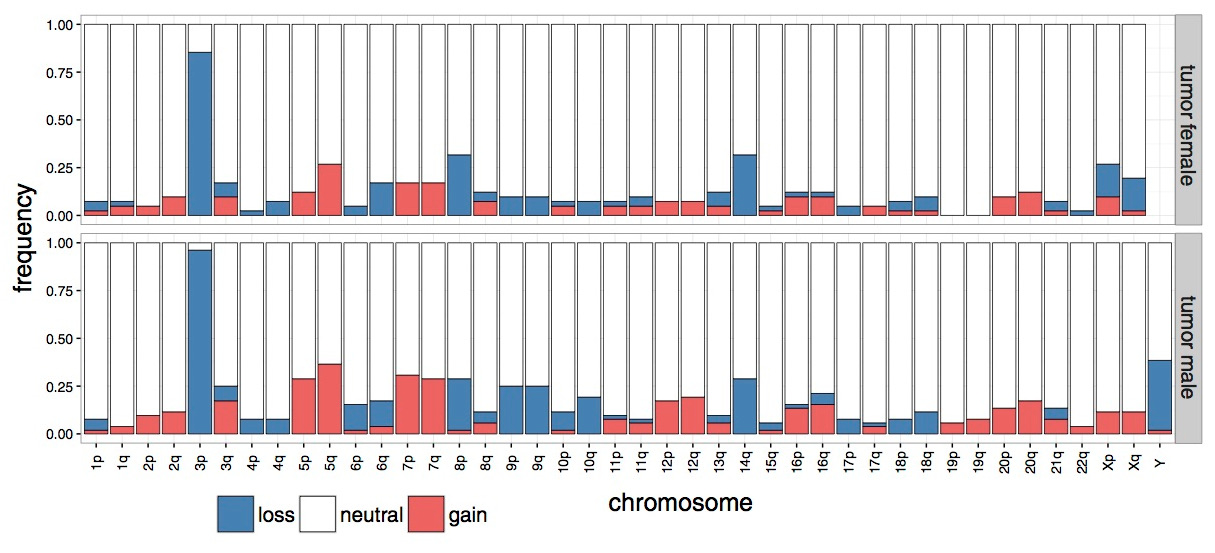
\includegraphics[width=.8\linewidth, page=1]{figures/LOY-fig1a.png}
    \caption{}
    \label{fig:loy1a}
  \end{subfigure}
  \begin{subfigure}[b]{\linewidth}
    \centering
    \includegraphics[width=.8\linewidth, page=2]{figures/Cagekid-LOY-fig.pdf}
    \caption{}
    \label{fig:loy1b}
  \end{subfigure}
  \caption[Copy number analysis in ccRCC.]{{\bf Copy number analysis in ccRCC.} {\small a) Bar graphs show the frequency of copy number variations across the genome in ccRCC tumors.
Frequencies are presented in samples from female and male cases separately.
b) Status of chromosome Y in DNA isolated from tumors (Y-axis) and patient-matched peripheral blood (X-axis) is shown for individual male subjects.
In samples affected by LOY, the normalized coverage of chromosome Y, shown on Y and X axes for tumor and normal samples, respectively, is lower than the expected value of 0.5.
The color codes define patient groups with different states for LOY.}}
\end{figure}

\paragraph{LOY is a whole-chromosome event}

Given the high prevalence of LOY in tumors and peripheral DNA of male patients, we further analyzed LOY in our sample series, particularly whether the observed LOY spans the whole chromosome or is focal.
Analysis of sequencing read coverage along chromosome Y showed that the loss is observed throughout the chromosome in samples affected by LOY (Fig. \ref{fig:loy2a}), suggesting that the deletion affects the whole chromosome.
Based on availability of DNA, we subjected samples from seven of the patients affected with somatic LOY to verification by an orthogonal Y-Chromosome deletion detection assay surveying the presence of twenty specific regions of the Y chromosome by polymerase chain reaction (PCR) (see \nameref{sec:loymethods}).
Somatic LOY at the chromosomal level was confirmed in all examined tumors, evident from an attenuated amplification of Y-chromosome-specific loci in DNA isolated from tumor samples compared to that of the matched constitutional DNA.
This pattern was not observed in samples of other male patients who had not been identified as being affected by somatic LOY based on the analysis of their WGS data (Fig. \ref{fig:loy2b}).

\begin{figure}[htp]
  \begin{subfigure}[b]{\linewidth}
    \centering
    \includegraphics[width=.7\linewidth, page=3]{figures/Cagekid-LOY-fig.pdf}
    \caption{}
    \label{fig:loy2a}
  \end{subfigure}
  \begin{subfigure}[b]{\linewidth}
    \centering
    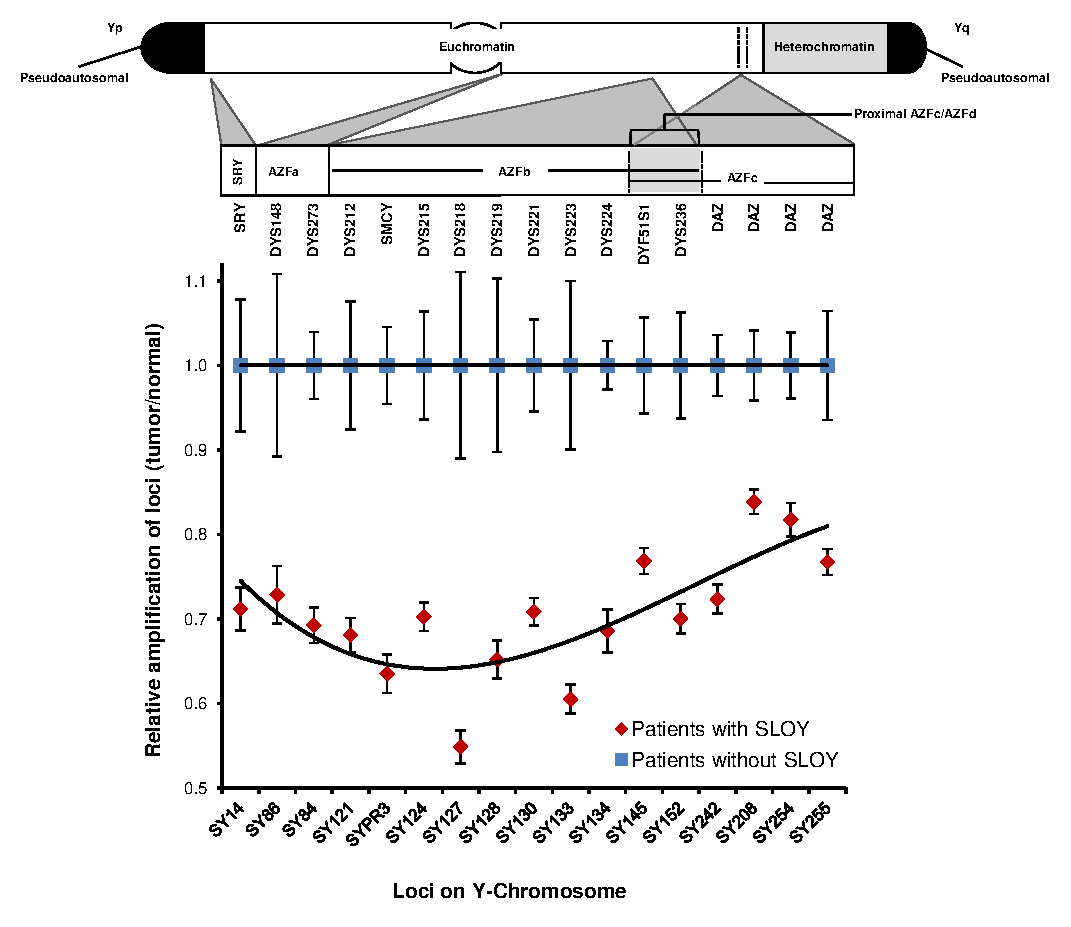
\includegraphics[width=.8\linewidth]{figures/LOY-fig2b.pdf}
    \caption{}
    \label{fig:loy2b}
  \end{subfigure}
  \caption[LOY affects whole chromosome.]{{\bf LOY affects whole chromosome.} {\small a) Sequencing coverage across chromosome Y is shown in constitutional DNA samples without (top) and with LOY (middle), and in a tumor sample with LOY (bottom).
b) The cartoon on top depicts the location of the loci examined by PCR on Y chromosome.
The dot graph on bottom shows average of relative amplification values (Tumor/normal samples of the same patient) for each locus in patients with (red) and without (blue) somatic LOY (
SLOY).
Error bars show the range across patients of each group.}}
\end{figure}


To confirm these findings, we screened tumor and matched control DNA sample pairs of an additional 48 male ccRCC patients (validation set) for LOY using the above PCR-based assay.
This analysis revealed somatic LOY in 20 (42.7\%) of the validation sample set, demonstrating that this is a common genomic aberration in ccRCC, detected in 39.6\% overall (discovery and validation sets; n$=$100) of male ccRCC patients (Fig. \ref{fig:loyS2}).
Analysis of association between somatic LOY and clinical annotations including tumor stage or grade did not show any significant relationships.

\paragraph{LOY results in downregulation of epigenetic modifier genes}

We further examined the possible effect of somatic LOY at the RNA level by interrogating a RNA-Seq dataset on gene expression in normal and tumor samples from male patients within the discovery set\cite{Scelo2014}.
We found that 11 genes had significantly different patterns of expression in tumors of the patients with and without somatic LOY (false-discovery rate (FDR)$<$0.01; Supplementary Table \ref{tab:loyS2}).
These 11 genes were located on chromosome Y, and while expressed in normal kidney tissue, exhibited lower expression in tumors of patients harboring somatic LOY, indicating that this aberration may have functional consequences through deregulation of the affected genes.
Moreover, the level of expression of each gene was found to be inversely correlated to the proportion of cells affected by LOY (Fig. \ref{fig:loy3}).
This observation was confirmed using gene expression data generated by microarrays, which was available for 29 tumors of the validation set\cite{Wozniak2013} (Fig. \ref{fig:loyS3}).
We surveyed the list of genes affected for potential functionally-relevant candidates.
Among these genes, {\it TMSB4Y} has recently been identified as a tumor suppressor gene downregulated in male breast cancers\cite{Wong2015}, but not connected to ccRCC.
Likewise, deletion of {\it KDM5D} has been detected in 52\% of prostate cancers\cite{Perinchery2000}.
{\it KDM5D} encodes a lysine-specific histone H3 demethylase, which plays an important role in epigenetic regulation\cite{Lee2007}.
Furthermore, it has been shown that knockdown of {\it KDM5D} through RNA-interference (RNAi) increases cell proliferation and reduces apoptosis in prostate cancer\cite{Jangravi2015}, suggesting a tumor suppressor function for this gene.
Intriguingly, {\it KDM5C}, the X-linked homologue of {\it KDM5D} is recurrently mutated in ccRCC\cite{Scelo2014,Dalgliesh2010,Creighton2013}, and its inactivation leads to genomic instability in ccRCC through deregulation of H3K4 methylation\cite{Rondinelli2015}.
{\it KDM5D} shows 85\% sequence identity to {\it KDM5C} and the products of these two genes possess a similar function in demethylating tri-methyl H3K4\cite{Lee2007,Rondinelli2015}.
Given this functional similarity, we surveyed the mutational status of {\it KDM5C} in our discovery set, and investigated possible relationships between mutational status of {\it KDM5C} and {\it KDM5D} in tumors of male patients.
In female patients, {\it KDM5C} was deleted in tumors of 7 cases through somatic LOX, and was affected by focal somatic deletions in two additional patients.
Furthermore, somatic mutations of {\it KDM5C} were present in tumors of 3 patients who were also affected with LOX (P$=$0.003, Fisher's exact test, Fig. \ref{fig:loyS4}).
Overall, {\it KDM5C} was affected with somatic genomic aberrations in 9 out of 41 (22\%) female cases.
As {\it KDM5C} escapes the X-inactivation\cite{Agulnik1994}, the concomitant mutations of {\it KDM5C} and LOX in the same tumors may suggest that this gene is a classical tumor suppressor affected with bi-allelic inactivation in ccRCC.
In male cases, we identified {\it KDM5C} mutations in tumors of 3 patients (5.8\%), of which one was also affected by somatic LOY (Fig. \ref{fig:loyS4}).
We did not detect any mutation or a focal CNV affecting {\it KDM5D} in tumors of the male patients who did not exhibit LOY.

\begin{figure}[ht]
  \centering
  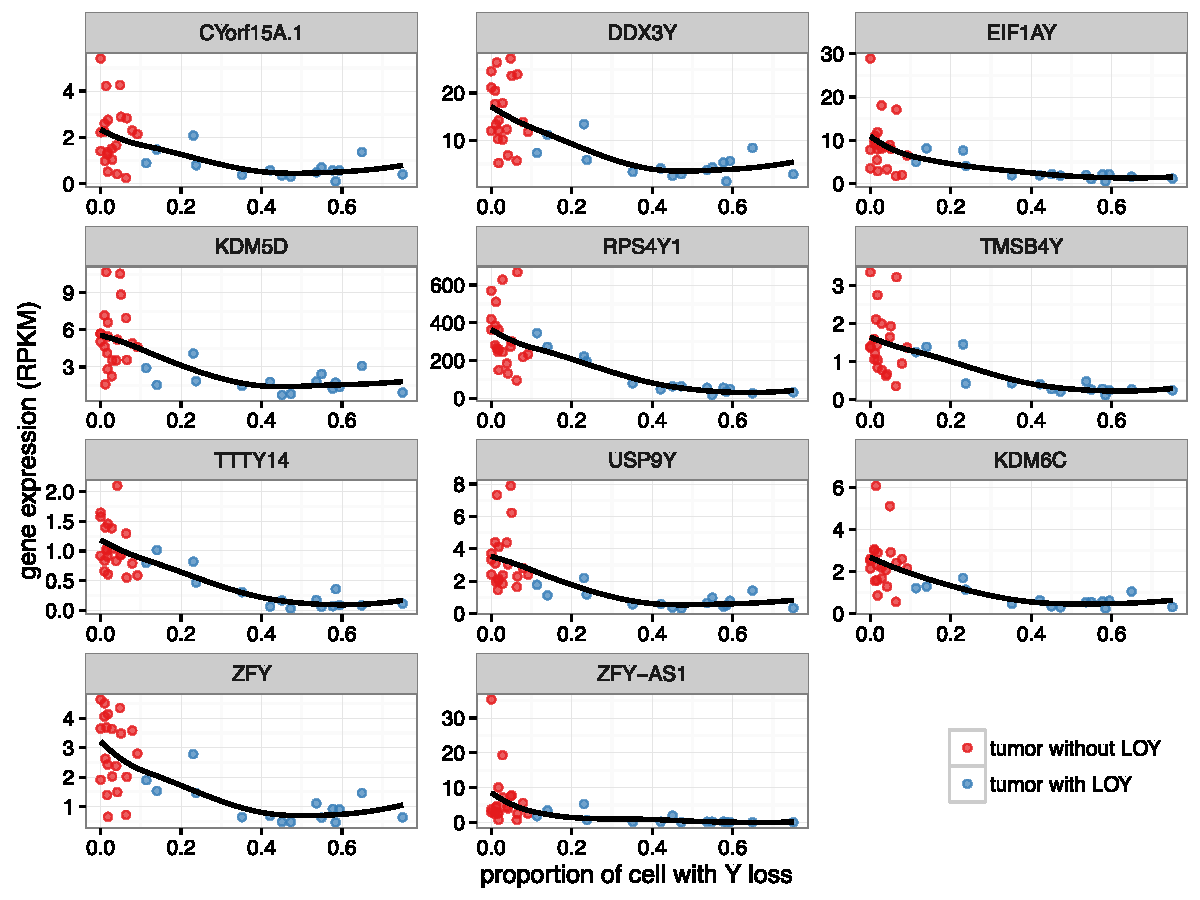
\includegraphics[width=.8\linewidth]{figures/LOY-fig3.pdf}
  \caption[Somatic LOY leads to downregulation of Y-linked genes.]{{\bf Somatic LOY leads to downregulation of Y-linked genes.} {\small Expression of Y chromosome genes downregulated in patients affected by somatic LOY is compared to the proportion of cells estimated to harbor somatic LOY in individual tumor samples.}}
  \label{fig:loy3}
\end{figure}

Our list of LOY-associated down-regulated genes (Supplementary Table \ref{tab:loyS2}) includes another epigenome modifier with an X-linked homologue that is also recurrently mutated in ccRCC; {\it UTY/KDM6C}.
{\it KDM6C} demethylates H3K27, a function similar to that of {\it KDM6A}\cite{Walport2014}.
These genes also share over 83\% in sequence similarity, resulting in highly conserved active sites in their products.
Mutations of {\it KDM6A} leading to its inactivation have been recurrently observed in ccRCC\cite{Dalgliesh2010,VanHaaften2009}, highlighting this gene as a potential key tumor suppressor in renal cancer.
In addition to being affected by somatic LOX in 7 female patients, {\it KDM6A} was also affected by focal deletion in a female patient in our cohort.

\paragraph{{\it KDM5D} expression reduces viability of renal cancer cells}

Given the reported tumor-suppressive function of {\it KDM5D} in prostate cancer\cite{Jangravi2015}, and of its X-link homolog {\it KDM5C} in renal cancer\cite{Rondinelli2015}, we set out to examine whether {\it KDM5D} expression has an anti-tumor activity in renal cancer.
We first evaluated {\it KDM5D} expression levels in several renal cancer cell lines, which have been derived from tumors resected from male patients.
Amongst cell lines examined, ACHN cell line did not show any expression for {\it KDM5D} (Fig. \ref{fig:loy4}a).
This observation was in line with a previous study reporting the loss of chromosome Y in ACHN cell line\cite{DuManoir1993}.
We therefore selected this cell line for functional analysis of {\it KDM5D} expression.
Ectopic expression of {\it KDM5D} cells reduced cell viability to 65\% as compared to control transfection (Fig. \ref{fig:loy4}b-c), suggesting the potential involvement of {\it KDM5D} depletion in renal cancer pathology.

\begin{figure}[ht]
  \centering
  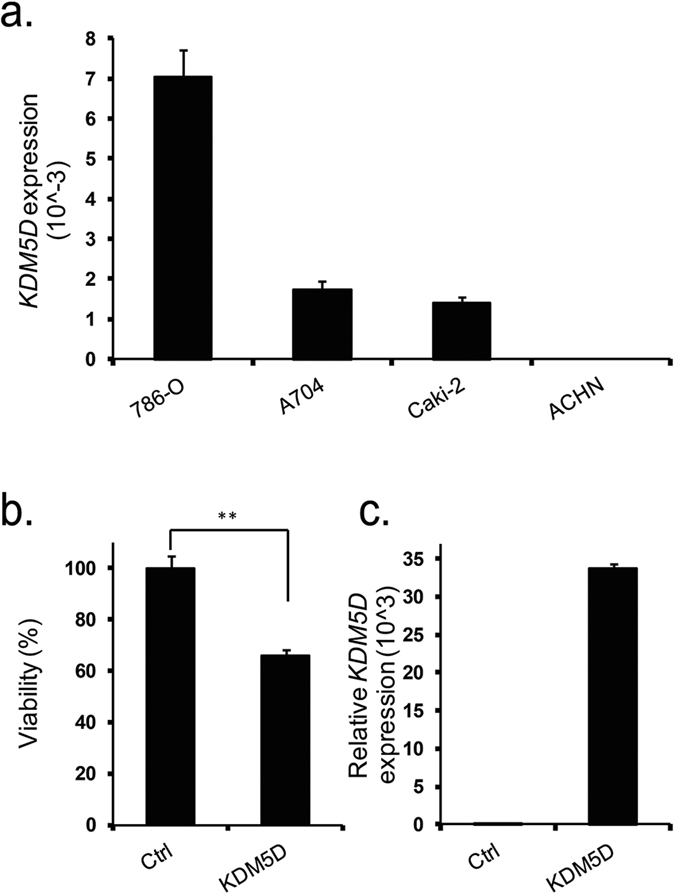
\includegraphics[width=.5\linewidth]{figures/LOY-fig4.png}
  \caption[Effect of {\it KDM5D} on viability of renal cancer cells.]{{\bf Effect of {\it KDM5D} on viability of renal cancer cells.} {\small a) Expression levels of {\it KDM5D} mRNA in renal cancer cell lines derived from tumors procured from male patients, as measured by qRT-PCR.
{\it GAPDH} served as a housekeeping gene for measurement of relative gene expression.
b) Over expression of {\it KDM5D} in ACHN cell line reduces cell viability.
Values are the mean $\pm$ SD of six independent experiments.
**$P<0.01$ when compared to the corresponding results from control (ctrl) (Mann-Whitney U test).
c) Over expression of {\it KDM5D} following transfection was confirmed using qRT-PCR.}}
  \label{fig:loy4}
\end{figure}

\section{Conclusions}

Emerging data emphasizes an association between LOY in peripheral blood and higher risk of cancer\cite{Forsberg2014}.
Likewise focal or chromosome-level somatic LOY occurs recurrently in different malignancies; however, current knowledge of mechanisms by which LOY may contribute to cancer is limited.
Recent genomic studies of ccRCC have highlighted the importance of molecular aberrations that impair the function of chromatin remodeling and epigenetic modifiers in ccRCC development\cite{Carvalho2014,Rondinelli2015,Kakarougkas2014,Simon2014,Pfister2014,Riazalhosseini2016}.
Our study expands these findings by highlighting the prevalence of somatic LOY among men affected by ccRCC, and suggesting a functional relevance for this aberration through down-regulation of previously unrecognized epigenetic modifiers {\it KDM5D} and {\it KDM6C}.
Given the functional similarities between these genes and their X-linked homologs, it is plausible that down-regulation of {\it KDM5D} and {\it KDM6C}, through somatic LOY, may contribute to ccRCC development or progression.
Our {in vitro} data shows that over expression of {\it KDM5D} in cancer cells that are affected by LOY reduces cell viability.
These findings indicate that down-regulation of {\it KDM5D} through LOY may contribute to the pathogenesis of renal cancer.
However, further detailed analysis through future functional studies is warranted to understand the exact function and pathway context of {\it KDM5D} in renal cancer.

\section{Methods}
\label{sec:loymethods}

\paragraph{Patient samples and DNA isolation}
 Clinical information for patients included in this study is presented in Supplementary Table \ref{tab:loyS1}.
Patients undergoing nephrectomy for suspected renal cancer during the period December 2008 to March 2011 at St James's University Hospital in Leeds, UK; University Hospital Motol, Prague, Czech Republic; Masaryk Memorial Cancer Institute, Brno, Czech Republic; Th. Burghele Hospital, Bucharest, Romania; and N. N. Blokhin Cancer Research Centre, Moscow, Russia, were recruited to the study after informed consent was obtained.
Recruitment in Central and Eastern Europe was coordinated by the International Agency for Research on Cancer (IARC).
All experiments and methods were performed in accordance to the ethics guidelines from the International Cancer Genome Consortium (ICGC) and to the relevant national regulations and with sampling and clinical data collection being undertaken according to predefined standard operating procedures (SOPs) based on guidelines from ICGC.
Ethical approvals were obtained from the Leeds (East) Local Research Ethics Committee, the IARC Ethics Committee, as well as from local ethics committee for recruiting centers in Czech Republic, Romania, and Russia.
DNA from fresh-frozen tumor tissue samples and buffy coat was isolated using Autopure (Qiagen) as described previously\cite{Scelo2014}, and were quantified by Quant-iT PicoGreen dsDNA Assay Kit (Invitrogen, ON, CAN).

\paragraph{Inference of LOY from WGS data}

WGS data of tumor and blood DNA samples studied here were reported previously\cite{Scelo2014}.
To detect aneuploidy and LOY from WGS data, we first measured read coverage across the genome in 5 Kbp bins.
In each sample, the coverage was normalized by the median coverage across the autosomes.
We then estimated, for each sample, the median normalized coverage in each chromosome arm.
The only exception was chromosome Y which was considered as a whole.
In order to avoid noise due to mappability issues, we used only the top 1000 bins with the lowest median divergence from the expected baseline in the normal samples.
We used this normalized median coverage per chromosome arm to test aneuploidy in each sample.
For each chromosome arm (or chromosome Y), a mixture of two Gaussian distributions was fitted to the empirical distribution of the median normalized coverage across samples.
The main Gaussian was used as the null distribution (Fig. \ref{fig:loyS5}) to derive P-values.
A chromosome arm was flagged as aneuploid if the Bonferonni-adjusted P-value was smaller than 0.01 and at least 10\% of cells were affected.
The proportion of cell with aneuploidy was estimated as the proportion of missing/excess coverage.
For LOY, we expect a normalized coverage of 0.5 and the proportion of cells with LOY was (0.5-coverage)/0.5.

We used a logistic regression to test the association of LOY with age.
Finally, the CNVs used for {\it KDM5C} or {\it KDM6A} deletion investigation were detected by {\sf PopSV}\cite{Monlong034165} using the normal samples as reference and 5 Kbp bins.

\paragraph{PCR-based detection of LOY}

To examine the status of LOY in DNA of tumor and blood samples, Y Chromosome Deletion Detection System assay, Version 2 (Promega, WI, USA) was used as instructed by the manufacturer.
Briefly, 20 specific regions of the Y chromosome were amplified by PCR using 5 multiplex master mixes, and PCR products were loaded on a QIAxcel instrument (Qiagen, ON, CAN).
Densities of PCR products were estimated by BioCalculator software (v.3.2) and a normalization was performed by the control primer pair included in each multiplex master mix to control the amplification efficacy.
We also included samples from three male subjects without LOY and one female sample to control the performance of the assay.
Similar to the analysis on WGS data, the probes were first normalized by the median probe amplification value across the normal samples.
Then the median of the normalized amplification was computed for each sample.
It summarized the overall amplification of chromosome Y in each sample.
These values were used to produce Fig. \ref{fig:loyS2} and to identify LOY.
Following the same analysis as for the WGS data, the mixture of Gaussian distributions was fitted on the normalized amplification of the normal samples.
Samples which deviated significantly (P$<$0.01) from the expected amplification and with an estimated proportion of affected of cells \textgreater{}10\% were flagged as being affected by LOY.

\paragraph{Gene expression analysis}

Transcriptome profiles of the tumor samples included in this study (previously reported in our earlier publication\cite{Scelo2014}), were used to examine differential gene expression between male subjects affected with somatic LOY and those without this abnormality.
RNA-seq data was available for tumors of 34 patients, of which 21 had RNA-seq for matched normal kidney samples.
Differentially expressed genes between tumors affected with somatic LOY and those without this abnormality were identified using Student's T-Test on log2-transformed RPKM data, and the Benjamini-Hochberg method was used to correct multiple testing.
Genes with a FDR$<$ 0.01 were considered differentially expressed.
A linear regression was used to test the association between the proportion of cells with somatic LOY and gene expression (RPKM).

Gene expression microarray data for 29 tumors of validation samples had previously been reported\cite{Wozniak2013}, and were used to confirm the anti-correlation between the proportion of cells with somatic LOY and gene expression levels (log2 intensity).

\paragraph{Cell viability assay}

Renal cancer cell lines 786-O, A704, Caki-2, ACHN were obtained from ATCC (Rockville, USA) and cultured in RPMI, EMEM and McCoy medium supplemented with 10\% (v/v) fetal bovine serum (FBS), 100 U/ml penicillin and 100 lg/ml streptomycin.
Cells were incubated at 37C and 5\% (v/v) CO2.
For viability assays, 5000 cells were transfected with 100 ng of either {\it KDM5D} cDNA-expressing (courtesy of Dr.
Stephane Richard) or control empty vector (Sigma, Oakville, Canada) in 96-well plates using Lipofectamine 3000 (Invitrogen) according to the manufacturer's instructions.
CellTiter-Glo assay (Promega, WI, USA) was used to assess cell viability after 72 hours post-transfection.

\paragraph{Quantitative real-time PCR (qRT-PCR)}

Total RNA was extracted from cells using miRNeasy kit (Qiagen, Toronto, Canada) according to the supplier protocols.
1 $\mu$g RNA was reverse transcribed into complementary DNA (cDNA) using Transcriptor First Strand cDNA Synthesis Kit (Roche, Laval, Canada) following instructions provided by the manufacturer.
Real-time PCR reactions were prepared using LightCycler 480 SYBR green I master kit (Roche), and were run on a LightCycler 480 instrument (Roche) according to the manufacturer's recommendations.
Triplicate PCR reactions were performed for each sample to ensure reliability.
Expression of {\it KDM5D} mRNA was normalized to the expression of the housekeeping gene {\it GAPDH}, and was reported as $2^{- \Delta C t}$.
All the primers were purchased from IDT (Coralville, IA, US).
The sequences of primers were \verb!CGTGGAAGGACTCATGACCA! ({\it GAPDH} forward), \verb!GCCATCACGCCACAGTTTC! ({\it GAPDH} reverse), \verb!CGCAGCTTTGAAGAGCTAAG! ({\it KDM5D} forward) and \verb!CAGCTGTGGAGTGTCCATCC! ({\it KDM5D} reverse).

\section{Acknowledgments}

This study was supported by funding from EU FP7 under grant agreement number 241669 (the CAGEKID project, \href{cagekid}{http://www.cng.fr/cagekid}), and funding from Génome Québec as well as Ministère de l'Enseignement supérieur, de la Recherche, de la Science et de la Technologie (MESRST).
We also acknowledge the support of Cancer Research UK Centre and ECMC infrastructure funding in Leeds for contributions to sample collection.
The Czech-Brno group was supported by MH CZ - DRO (MMCI, 00209805).
JM is supported by funds from National Sciences and Engineering Research Council (NSERC-448167-2013).

% \section{Author Contributions}

% Y.R. conceived the study and designed the experiments with contribution from G.B. N.V., P.H., L.E., I.H., A.B., V.J., H.K., L.F., M.N., D.M., Vi.J., D.Z., A.M., P.B., G.S. and R.E.B. were responsible for patient selection, sample collection, sample preparation and pathological reviews. M.A. and N.N. prepared DNA, performed experiments to detect LOY and analyzed the data with contribution from P.J. J.M. developed the computational methods for WGS analysis, analyzed WGS data and generated the figures. P.P., R.S.L., P.J. and Al.B. performed the gene expression analysis. M.L. provided critical advice on data analysis and statistical approaches. M.S. and P.J. performed functional analysis with cell line models. M.A. and Y.R. wrote the manuscript, with assistance from J.T., G.S. and R.E.B. 

%%% Local Variables:
%%% mode: latex
%%% TeX-master: "../main"
%%% End:


\singlespacing
\chapter[Detection of CNVs in Epilepsy Patients]{Population-Based Detection of CNVs in Epilepsy Patients}
\label{chap:epi}
\doublespacing
\section*{Preface: Bridging Text between Chapters 2 and 3}
\addcontentsline{toc}{section}{Preface: Bridging Text between Chapters 2 and 3}


In this chapter, the population-based approach used to detect arm-level CNV was extended to the detection of small CNV across the genome.
Instead of testing one chromosomal arm at a time, the genome is tiled and each region is tested for CNV using the same strategy: a set of reference samples is used to deal with technical variation.
By better integrating technical variation, our goal is to improve the robustness and sensitivity of the CNV detection.
Notably, this chapter introduces {\sf PopSV}, the CNV detection method implemented in the context of this thesis, and its application to a disease study.
{\sf PopSV} is later used in chapter \ref{chap:rep} to investigate CNVs in low-mappability regions.

In this Research Article published in {\it PLoS Genetics}\cite{Monlong2018}, we first introduce the rationale for the method: the presence of visible technical bias in WGS coverage data.
After an overview of the method, we show that it is more sensitive than other methods and avoids systematic calls.
Finally, we apply {\sf PopSV} to WGS data from 198 epilepsy patients and 301 controls and show CNV enrichments in exons and non-coding regions that potentially explain an important fraction of patients.
\nameref{append:epi} contains supplementary tables, figures and information.
\bigskip

\newpage
\singlespacing

\begin{center}
  \LARGE\bf Global characterization of copy number variants in epilepsy patients from whole genome sequencing
\end{center}
\bigskip

\large{Jean Monlong$^{1,2,*}$, Simon L. Girard$^{1,3,4,*}$, Caroline Meloche$^{4}$, Maxime Cadieux-Dion$^{4,5}$, Danielle M. Andrade$^{6}$, Ron G. Lafreniere$^{4}$, Micheline Gravel$^{4}$, Dan Spiegelman$^{7}$, Alexandre Dionne-Laporte$^{7}$, Cyrus Boelman$^{8}$, Fadi F. Hamdan$^{9}$, Jacques L. Michaud$^{9}$, Guy Rouleau$^{7}$, Berge A. Minassian$^{10}$, Guillaume Bourque$^{1,2,11,+}$, Patrick Cossette$^{4,+}$}
\bigskip

\footnotesize
$^{1}$ Department of Human Genetics, McGill University, Montr\'eal, H3A 1B1, Canada

$^{2}$ Canadian Center for Computational Genomics, Montr\'eal, H3A 1A4, Canada

$^{3}$ D\'epartement des sciences fondamentales, Universit\'e du Qu\'ebec \`a  Chicoutimi, Chicoutimi, G7H 2B1, Canada

$^{4}$ Centre de Recherche du Centre Hospitalier de l'Universit\'e de Montr\'eal, Montr\'eal, H2X 0A9, Canada

$^{5}$ Center for Pediatric Genomic Medicine, Children's Mercy Hospital, Kansas City, MO, USA

$^{6}$ Epilepsy Genetics Program, Division of Neurology, Toronto Western Hospital, University of Toronto, Toronto, Canada

$^{7}$ Montreal Neurological Institute, McGill University, Montr\'eal, H3A 2B4, Canada

$^{8}$ Division of Neurology, BC Children's Hospital, Vancouver, V6H 3N1, Canada

$^{9}$ CHU Sainte-Justine Research Center, Montr\'eal, H3T 1C5, Canada

$^{10}$ Division of Neurology, The Hospital for Sick Children, Toronto, M5G 1X8, Canada

$^{11}$ McGill University and G\'enome Qu\'ebec Innovation Center, Montr\'eal, H3A 1A4, Canada

$^+$Correspondence: guil.bourque@mcgill.ca or patrick.cossette@umontreal.ca

$^*$These authors contributed equally to this work


\normalsize
\doublespacing

\section{Abstract}
Epilepsy will affect nearly 3\% of people at some point during their lifetime. 
Previous copy number variants (CNVs) studies of epilepsy have used array-based technology and were restricted to the detection of large or exonic events. 
In contrast, whole-genome sequencing (WGS) has the potential to more comprehensively profile CNVs but existing analytic methods suffer from limited accuracy. 
We show that this is in part due to the non-uniformity of read coverage, even after intra-sample normalization. 
To improve on this, we developed {\sf PopSV}, an algorithm that uses multiple samples to control for technical variation and enables the robust detection of CNVs. 
Using WGS and {\sf PopSV}, we performed a comprehensive characterization of CNVs in 198 individuals affected with epilepsy and 301 controls. 
For both large and small variants, we found an enrichment of rare exonic events in epilepsy patients, especially in genes with predicted loss-of-function intolerance. 
Notably, this genome-wide survey also revealed an enrichment of rare non-coding CNVs near previously known epilepsy genes. 
This enrichment was strongest for non-coding CNVs located within 100 Kbp of an epilepsy gene and in regions associated with changes in the gene expression, such as expression QTLs or DNase I hypersensitive sites. 
Finally, we report on 21 potentially damaging events that could be associated with known or new candidate epilepsy genes. 
Our results suggest that comprehensive sequence-based profiling of CNVs could help explain a larger fraction of epilepsy cases. 


\section{Author Summary}
Epilepsy is a common neurological disorder affecting around 3\% of the population.
In some cases, epilepsy is caused by brain trauma or other brain anomalies but there are often no clear causes.
Genetic factors have been associated with epilepsy in the past such as rare genetic variations found by linkage studies as well as common genetic variations found by genome-wide association studies and large copy-number variants.
We sequenced the genome of $\sim$200 epilepsy patients and $\sim$300 healthy controls and compared the distribution of deletion (loss of a copy) and duplication (additional copy) of genomic regions.
Thanks to the sequencing technology and a new method that takes advantage of the large sample size, we could compare the distribution of small copy-number variants between epilepsy patients and controls.
Overall, we found that small variants are also associated with epilepsy.
Indeed, the genome of epilepsy patients had more exonic copy-number variants, especially when rare or affecting genes with predicted loss-of-function intolerance.
Focusing on regions around genes that have been previously associated with epilepsy, we also found more non-coding variants in epilepsy patients, especially deletions or variants in regulatory regions.
Finally, we provide a list of 21 regions in which we found likely pathogenic variants.

\section{Introduction}
Structural variants (SVs) are defined as genetic mutations affecting more than 50 base pairs and encompass several types of rearrangements: deletion, duplication, novel insertion, inversion and translocation.
Deletions and duplications, which affect DNA copy number, are collectively known as copy number variants (CNVs).
SVs arise from a broad range of mechanisms and show a heterogeneous distribution of location and size across the genome\cite{Hall2012,Sharp2006,Mills2011}.
Numerous diseases are caused by SVs with a demonstrated detrimental effect\cite{Conrad2010,Spielmann2013}.
While cytogenetic approaches and array-based technologies have been used to identify large SVs, whole-genome sequencing (WGS) has the potential to uncover the full range of SVs both in terms of type and size\cite{Zhao2013a,Pirooznia2015}.
SV detection methods that use read-pair and split read information\cite{Layer2012} can detect deletions and duplications but most CNV-focused approaches look for an increased or decreased read coverage, the expected consequence of a duplication or a deletion.
Coverage-based methods exist to analyze single samples\cite{Abyzov2011}, pairs of samples\cite{Boeva2011} or multiple samples\cite{Handsaker2015,Klambauer2012,Glusman2015} but the presence of technical bias in WGS remains an important challenge.
Indeed, various features of sequencing experiments, such as mappability\cite{Treangen2011,Teo2012}, GC content\cite{Benjamini2012}, replication timing\cite{Koren2014}, DNA quality and library preparation\cite{VanDijk2014}, have a negative impact on the uniformity of the read coverage\cite{Cheung2011}.

Epilepsy is a common neurological disorder characterized by recurrent and unprovoked seizures.
It is estimated that up to 3\% of the population will suffer from a form of epilepsy at some point during their lifetime.
Although the disease presents a strong genetic component that can be as high as 95\%, typical ``monogenic'' epilepsy is rare, accounting for only a fraction of cases\cite{Berkovic1998,Zara1995}.
Genetic factors have been associated with epilepsy in the past such as rare genetic variations found by linkage studies as well as common genetic variations found by genome-wide association studies\cite{Kasperaviciute2010a,Guo2012}
For example, a meta-analysis combining multiple epilepsy cohorts found positive associations with the disease\cite{InternationalLeagueAgainstEpilepsyConsortiumonComplexEpilepsies2014}, the strongest in {\it SCN1A}, a gene already associated with the genetic mechanism of the disease via linkage studies and subsequent sequencing\cite{Escayg2000} or more recently as harboring {\it de novo} variants\cite{Claes2003}.
Thanks to array-based technologies, surveys of large CNVs ($>$50 Kbp) first associated CNVs in genomic hotspots such as 15q11.2 and 16p13.11 with generalized epilepsy\cite{Helbig2009,DeKovel2010}.
Other studies have further shown the importance of large and \textit{de novo} CNVs as well as identified a few associations with specific genes\cite{Mefford2010,Helbig2014,Mefford2015,Addis2016,Biervert1998,Lal2015}.
Rare genic CNVs were typically found in around 10\% of epilepsy patients\cite{Mefford2011,Mefford2010,Addis2016} and CNVs larger than 1 Mbp were significantly enriched in patients compared to controls\cite{Mefford2011,Heinzen2010,Striano2012,Lal2015}.
Unfortunately, small CNVs and other types of SVs could not be efficiently or consistently detected using these technologies, hence much remains to be done.

To more comprehensively characterize the role of CNVs in epilepsy, we performed whole-genome sequencing of epileptic patients from the Canadian Epilepsy Network (CENet), the largest WGS study on epilepsy to date.
In the present study, we assessed the frequency of CNVs in epileptic individuals using 198 unrelated patients and 301 healthy individuals. Using this data, we showed that technical variation in WGS remains problematic for CNV detection despite state-of-the-art intra-sample normalization.
To correct for this and to maximize the potential of the CENet cohorts, we developed a population-based CNV detection algorithm called {\sf PopSV}.
Our method uses information across samples to avoid systematic biases and to more precisely detect regions with abnormal coverage.
Using two public WGS datasets\cite{Scelo2014,Boivin2013}, and additional orthogonal validation, we showed that {\sf PopSV} outperforms other analytical methods both in terms of specificity and sensitivity, especially for small CNVs.
Using this tool, we built a comprehensive catalog of CNVs in the CENet epilepsy patients and studied the properties of these potentially damaging structural events across the genome.


\section{Results}

\subsection*{Technical bias in read coverage}
We sequenced the genomes of 198 unrelated individuals affected with epilepsy and 301 unrelated healthy controls.
Because CNV detection relies on read coverage we first investigated the presence of technical bias and the value of standard corrections and filters (e.g. GC correction, mappability filtering).
The genome was fragmented in 5 Kb bins and we counted the number of uniquely mapped reads in each bin.
In contrast to simulated datasets, we found that the inter-sample mean coverage in each bin varied between genomic regions even after stringent corrections and filters (Fig. \ref{fig:wgsbias}).
Supporting this observation, the bin coverage variance across samples was also lower than expected and varied between regions (Fig. \ref{fig:bias:var}).
We also observed experiment-specific biases. In particular, some samples consistently had the highest, or the lowest, coverage across large portions of the genome (Fig. \ref{fig:bias:rank}).
These observations were not unique to our data and could also be observed in two public WGS datasets, and persisted even after correcting the GC bias and mappability using the more elaborate model from the {\sf QDNAseq} pipeline\cite{Scheinin2014} (Fig. \ref{fig:wgsbias2}).
Our results across multiple samples suggest that existing GC bias and mappability corrections\cite{Scheinin2014} cannot correct completely the technical variation in read coverage.
This fluctuation of coverage has implications for CNV detection approaches that assume a uniform distribution\cite{Boeva2011,Abyzov2011,Xi2011} after standard bias correction and will lead to false positives.

\begin{figure}[!h]
  \begin{subfigure}[b]{.3\linewidth}
    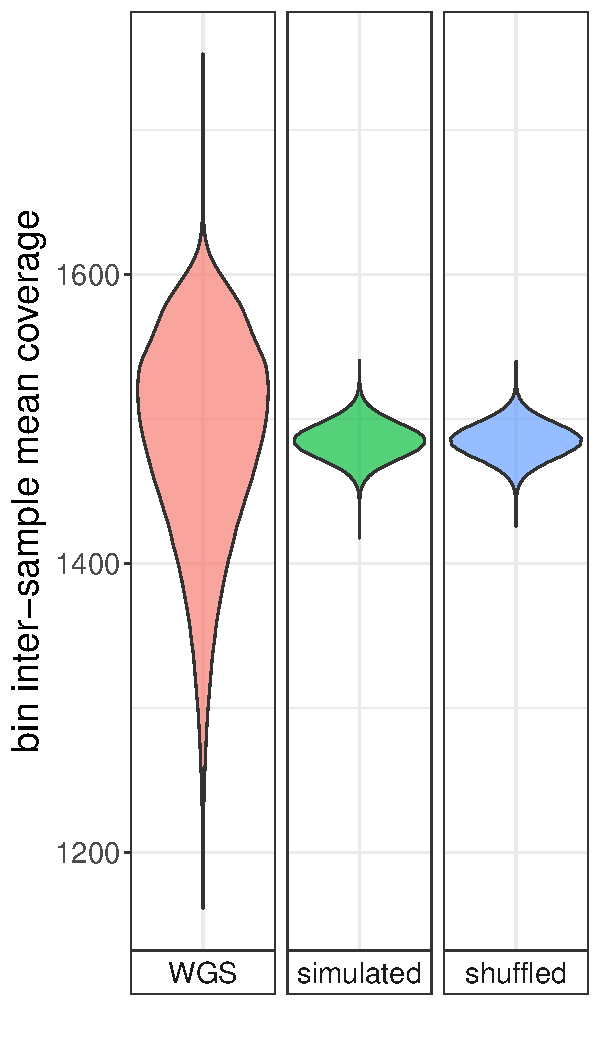
\includegraphics[width=\linewidth,page=1]{figures/epilepsy-biasWGS-thin.pdf}
    \caption{}
    \label{fig:wgsbias}
  \end{subfigure}
  \unskip\ \vrule\
  \begin{subfigure}[b]{.7\linewidth}
    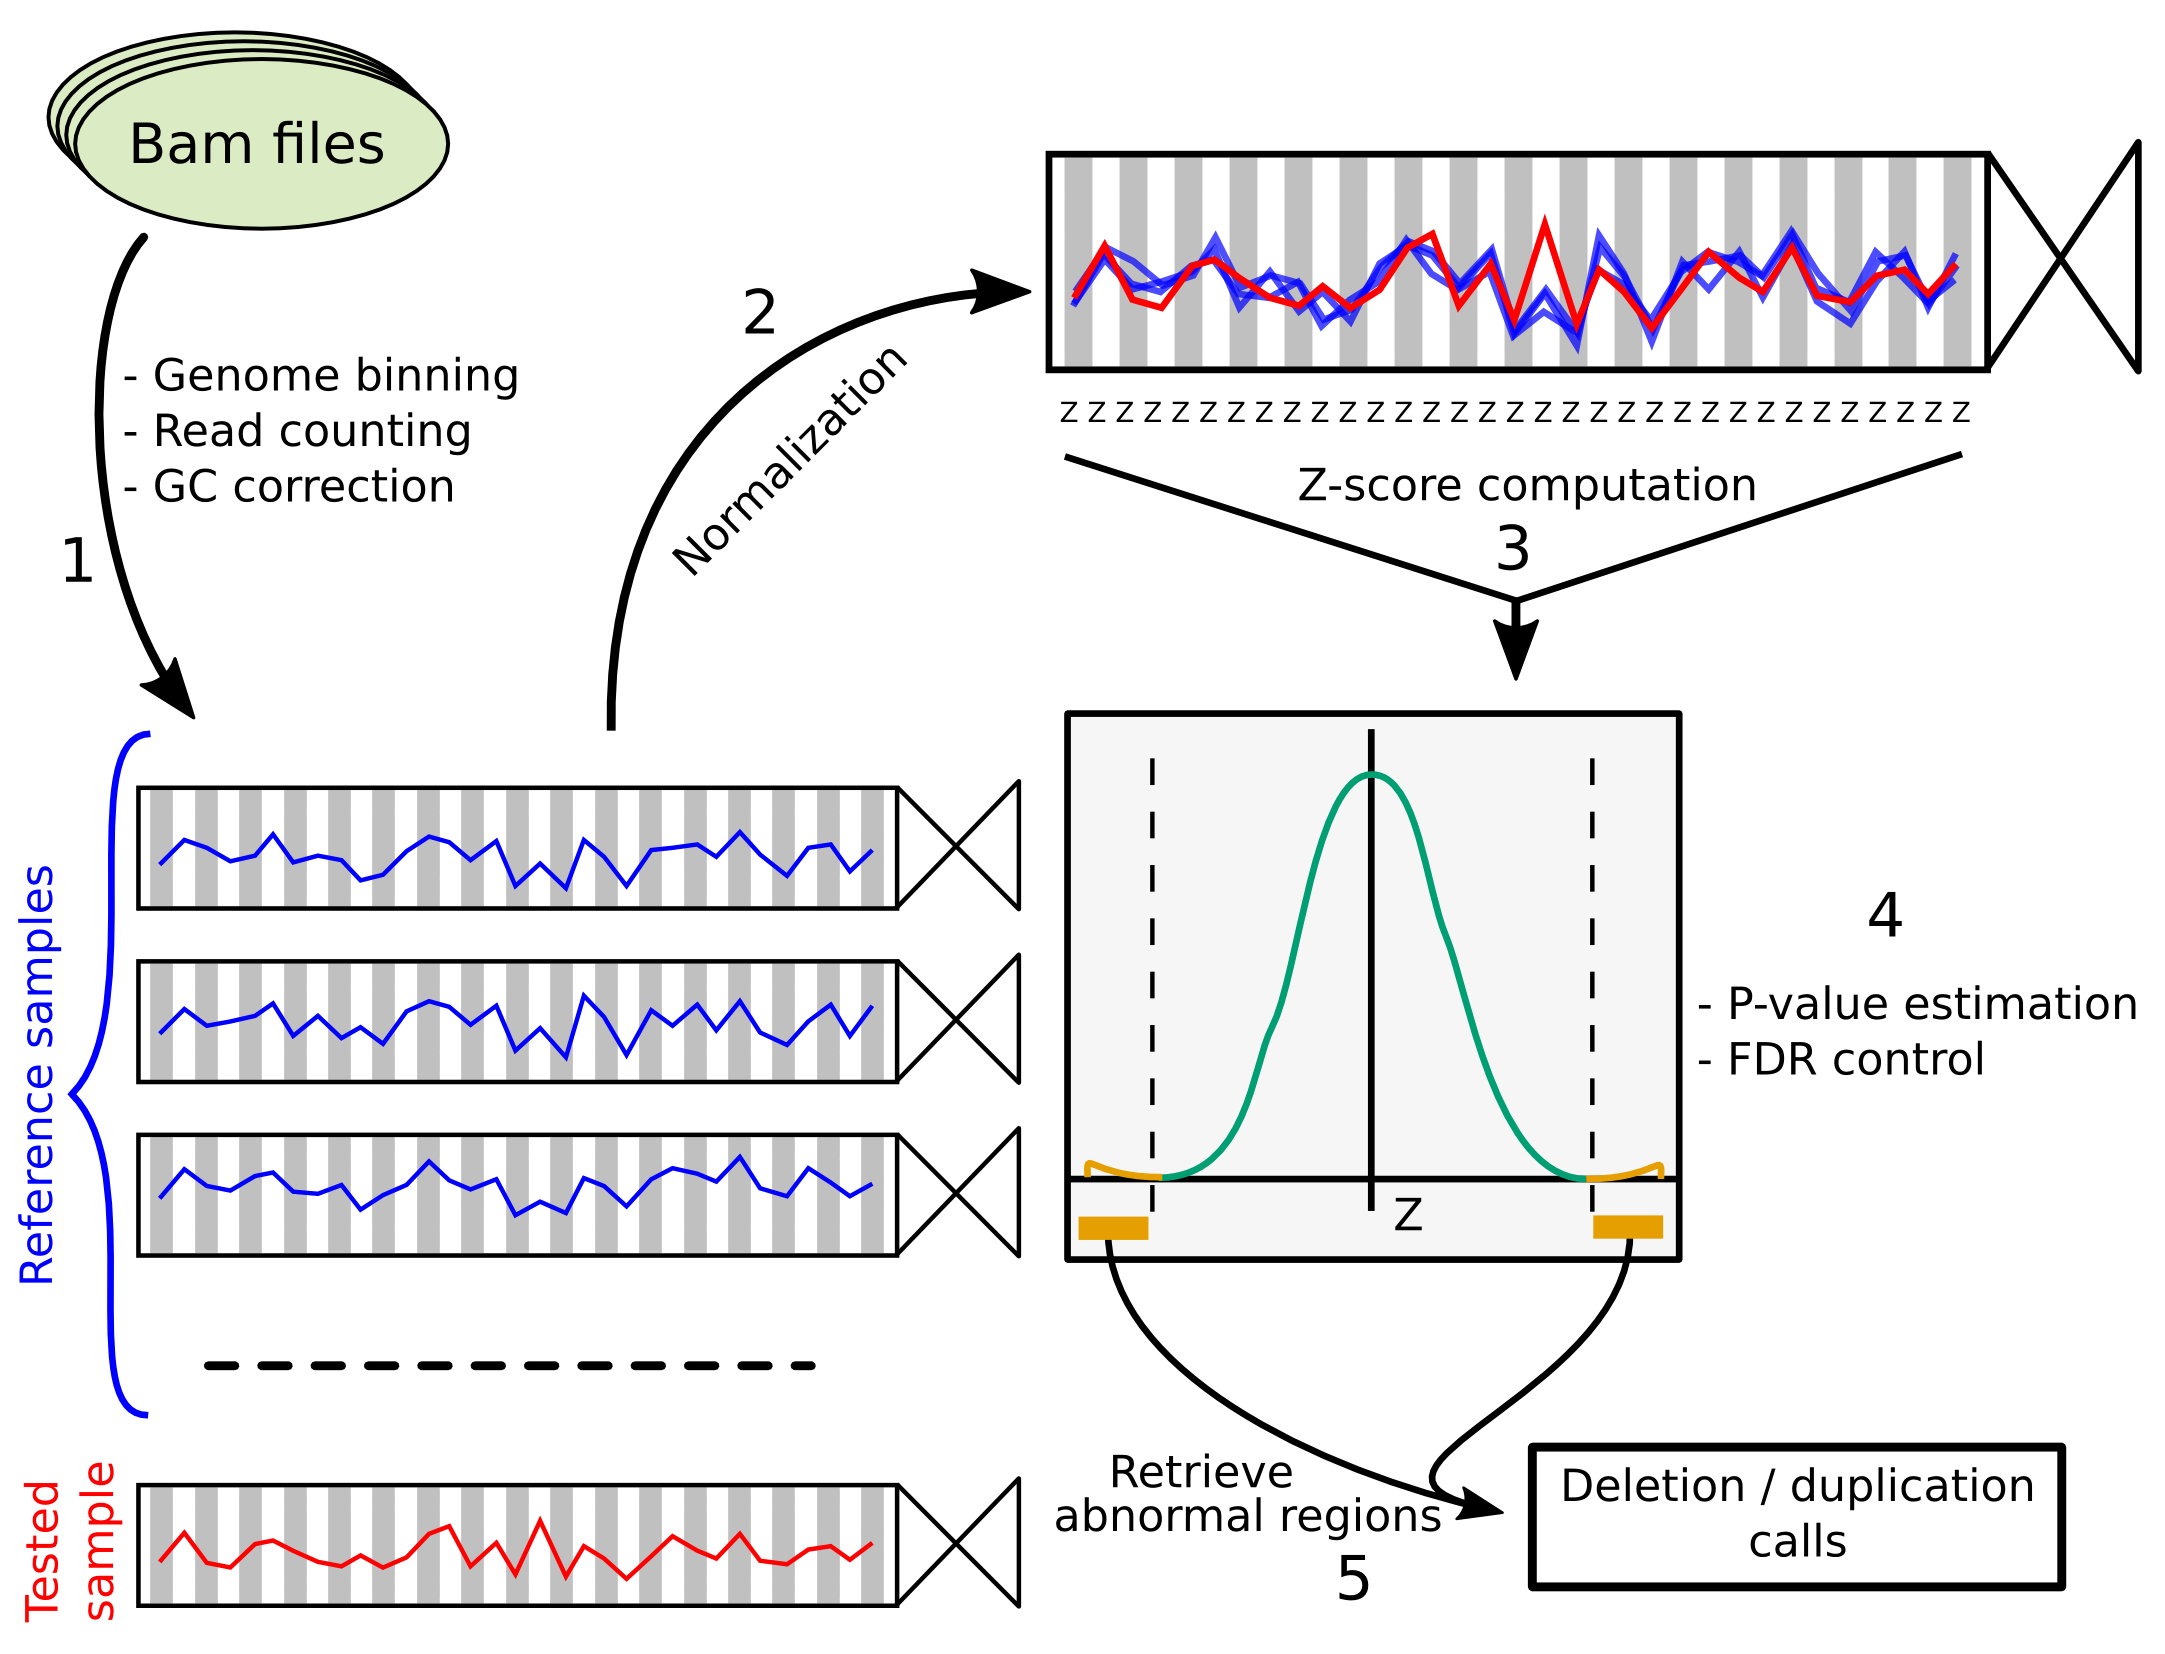
\includegraphics[width=\linewidth]{figures/PopSVworkflow.png}
    \caption{}
    \label{fig:popsv}
  \end{subfigure}
  \unskip \hrule\
  \medskip

  \begin{subfigure}[b]{\linewidth}
    \includegraphics[width=.5\linewidth, page=2]{figures/twin-benchmark-long.pdf}
    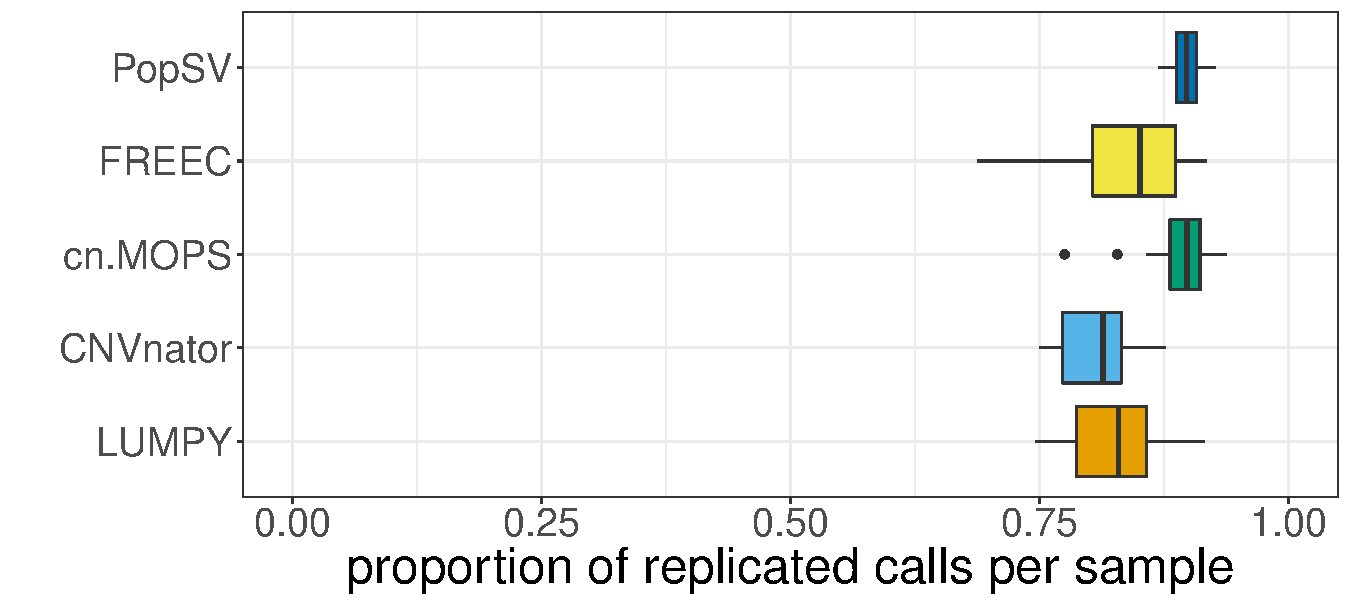
\includegraphics[width=.5\linewidth, page=1]{figures/twin-benchmark-long.pdf}
    \caption{}
    \label{fig:twinconc}
  \end{subfigure}
  \caption[{\sf PopSV} approach]{{\bf {\sf PopSV} approach. } {\small a) Technical bias across the genome remains after stringent correction and filtering. The distribution of the bin inter-sample mean coverage in the epilepsy cohort (red) is compared to null distributions (blue: bins shuffled, green: simulated normal distribution). b) {\sf PopSV} approach. First the genome is fragmented and reads mapping in each bin are counted for each sample and GC corrected (1). Next, coverage of the sample is normalized (2) and each bin is tested by computing a Z-score (3), estimating p-values (4) and identifying abnormal regions (5). c) Number and proportion of calls from a twin that was replicated in the other monozygotic twin.}}
\end{figure}


\subsection*{CNV detection with {\sf PopSV}}
To better control for technical bias, we developed {\sf PopSV}, a new SV detection method.
{\sf PopSV} uses read depth across the samples to normalize coverage and detect change in DNA copy number (Fig. \ref{fig:popsv}).
The normalization step here is critical since most approaches will fail to give acceptable normalized coverage scores (Fig. \ref{fig:bias:rank}).
Moreover, with global median/variance adjustment or quantile normalization, the remaining subtle experimental variation impairs the abnormal coverage test (Fig. \ref{fig:zscoreEx:worstZ}).
The targeted normalization used by {\sf PopSV} was found to have better statistical properties (Fig. \ref{fig:normComp}).
In order to assess the performance of our tool, we compared it to several algorithms\cite{Boeva2011,Abyzov2011,Klambauer2012,Layer2012} using a dataset that included monozygotic twins and also performed experimental validation of different types of predicted CNVs in the epilepsy cohort (see below).
We found that {\sf PopSV} performed as well or better in different aspects.
First, for several algorithms, a large proportion of the detected events in a typical sample were also identified in almost all samples (60\% of the calls found in $>$95\% of the samples, Fig. \ref{fig:freqmeth}).
{\sf PopSV}'s calls were better distributed across the frequency spectrum, hence more informative as we expect the relative frequency of disease-related variants to be rare.
In addition, the pedigree structure was more accurately recovered when the CNVs were used to cluster the individuals in the Twins dataset (Fig. \ref{fig:twinclust}).
The agreement with the pedigree was computed by the Rand index after clustering the individuals with three hierarchical clustering approaches (see \nameref{sec:suppmat:epipopsv}).
Looking at the replication between 10 pairs of monozygotic twins, {\sf PopSV} detected more replicated CNVs compared to other methods, while maintaining similar replication rates (Fig. \ref{fig:twinconc}).
The CNV calls were further filtered with gradually more stringent significance thresholds and {\sf PopSV} remained superior in term of number of replicated calls (Fig. \ref{fig:twinconcsig}).
When investigating the overlap of calls between different methods, we noticed that {\sf PopSV} was better recovering calls from {\sf CNVnator}\cite{Abyzov2011}, {\sf FREEC}\cite{Boeva2011}, {\sf cn.MOPS}\cite{Klambauer2012} or {\sf LUMPY}\cite{Layer2012}, especially if found by two or more methods (Fig. \ref{fig:twincallcomp}).
For example, around 92\% of the CNVs called by other methods were also found by {\sf PopSV} when focusing on calls found in at least two methods.
Similar results were also obtained in a cancer dataset where we looked for replicated germline CNVs in the paired tumor (Fig. \ref{fig:ckconc}).
Finally, we repeated the twin analysis using 500 bp bins and observed high consistency with the 5 Kbp calls (Fig. \ref{fig:compsize}).
These results suggest that {\sf PopSV} can accurately detect around 75\% of events that are as large as half the bin size used (see \nameref{sec:suppmat:epipopsv}).

\subsection*{CNVs in the CENet cohorts and experimental validation}
Having demonstrated the quality of the {\sf PopSV} calls, we applied our tool to the epilepsy and control cohorts.
The epilepsy cohort comprises 198 individuals diagnosed with either generalized (n=160), focal (n=32) or unclassified (n=6) epilepsy.
CNVs ranged from 5 Kbp to 3.2 Mbp with an average size of 9.98 Kbp.
We observed an average of 870 CNVs per individual accounting for 8.7 Mb of variant calls (Fig. \ref{fig:cnvs}).
This is around 9 times more variants and considerably smaller than in typical array-based studies\cite{Redon2006,Itsara2009}, such as the previous epilepsy surveys\cite{Mefford2011,Mefford2010,Helbig2014,Addis2016}, although a similar size distribution was previously obtained using denser arrays\cite{Conrad2010} but were never applied to epilepsy (Fig. \ref{fig:arraysize}).
Next, we annotated each variant using four public SV databases\cite{Sudmant2015a,Handsaker2015,Francioli2014,Sudmant2015} as well as an internal database of the germline calls from {\sf PopSV} in the two public datasets used earlier (see \nameref{sec:suppmat:epipopsv}).
For each CNV, we derived the maximum frequency across these databases and defined as rare any region consistently annotated in less than 1\% of the individuals (Fig. \ref{fig:cnvfreq}).
In total, we identified 12,480 regions with rare CNVs in the epilepsy cohort including: 8,022 (64.3\%) with heterozygous deletions, 21 (0.2\%) with homozygous deletions and 4,850 (38.9\%) with duplications.
Although the overall amount of rare CNVs was not higher in epilepsy patients, the proportion of deletion was significantly higher compared to controls ($\chi^2$ test: P-value $10^{-7}$).
Next, we selected 151 CNVs and further validated them using a Taqman CNV assay and Real-Time PCR.
To explore {\sf PopSV}'s performance across different CNV profiles, we selected variants of different types, sizes and frequencies.
We found that the calls were concordant in 90.7\% of the cases (Table \ref{tab:validationrates} and \ref{tab:validation}).
As expected, the estimated false positive rate was slightly higher for rare or smaller variants (12.1\% for rare CNVs; 15.1\% for CNV $<$20 Kbp).
Furthermore, we noted that calls supported by both {\sf PopSV} and {\sf LUMPY} (when available) had a similar validation rate as calls found by {\sf PopSV} only (86.2\% and 87.5\% respectively).

\begin{figure}[!h]
  \centering
  \begin{subfigure}[b]{.49\textwidth}
    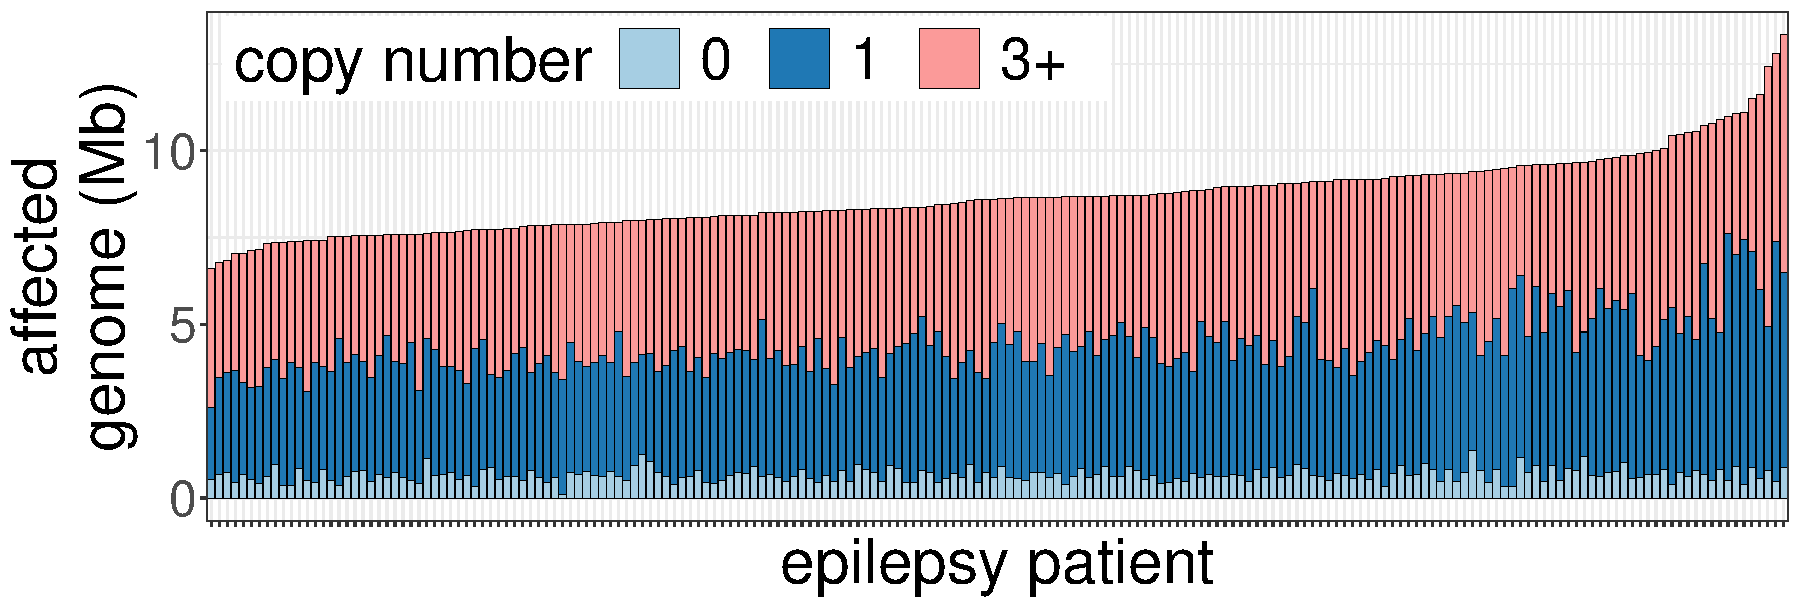
\includegraphics[width=\linewidth, page=1]{figures/epilepsy-CNVnumbers.pdf}
    \caption{}
    \label{fig:cnvs}
  \end{subfigure}
  \begin{subfigure}[b]{.49\textwidth}
    \includegraphics[width=\linewidth, page=3]{figures/epilepsy-CNVnumbers.pdf}
    \caption{}
    \label{fig:cnvfreq}
  \end{subfigure}
  \medskip
  
  \begin{subfigure}[b]{.9\textwidth}
    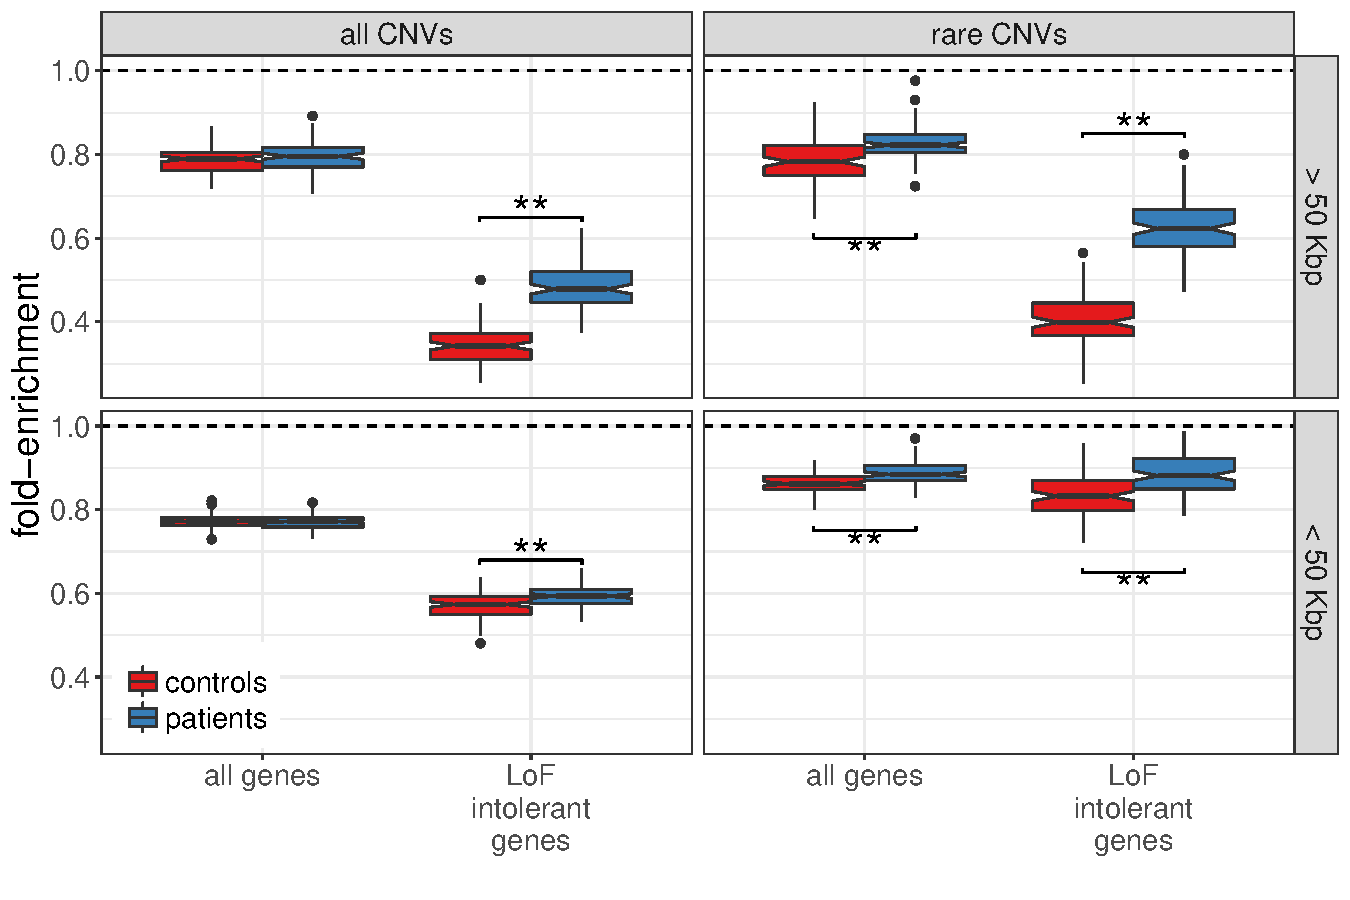
\includegraphics[width=\linewidth,page=1]{figures/epilepsy-enrichmentPatterns.pdf}
    \caption{}
    \label{fig:exenr}
  \end{subfigure}
  \caption[CNVs in the epilepsy and control cohorts.]{{\bf CNVs in the epilepsy and control cohorts.} {\small a) Regions with a CNV in each epilepsy patient. b) Each CNV in the CNV catalog of the epilepsy and control cohorts was annotated with its maximum frequency in five CNV databases. c) Enrichment in exonic sequence for all CNVs (left) and rare CNVs (right), larger than 50 Kbp (top) or smaller than 50 Kbp (bottom). The fold-enrichment (y-axis) represents how many CNVs overlap coding sequences compared to control regions randomly distributed in the genome.}}
\end{figure}

\begin{table}[!ht]
  \renewcommand{\arraystretch}{.7}
  \centering
  \caption[Real-Time PCR validation rates of {\sf PopSV} calls.]{{\bf Real-Time PCR validation rates of {\sf PopSV} calls.}}
  \begin{tabular}[c]{|l|r|r|}
    \hline
                            & Region & Validation rate \\
    \hline
    Total                   & 151    & 0.907           \\
    \hline
    CNV type                &        &                 \\
    $~~$Deletion            & 102    & 0.902           \\
    $~~$Duplication         & 49     & 0.918           \\
    \hline
    Frequency in databases   &        &                 \\
    $~~0$                   & 26     & 0.923           \\
    $~~(0,0.01]$            & 24     & 0.833           \\
    $~~(0.01,1]$            & 101    & 0.921           \\
    \hline
    Carrier in CENet cohorts&        &                 \\
    $~~1$                   & 21     & 0.857           \\
    $~~2$                   & 19     & 0.947           \\
    $~~>2$                  & 111    & 0.910           \\
    \hline
    Size (Kbp)              &        &                 \\
    $~~<20$                 & 73     & 0.849           \\
    $~~(20,100]$            & 38     & 0.974           \\
    $~~>100$                & 40     & 0.950           \\
    \hline
  \end{tabular}
  \begin{flushleft}
    Number and proportion of regions validated for CNVs of different types, sizes and frequencies.
  \end{flushleft}
  \label{tab:validationrates}
\end{table}


\subsection*{CNV enrichment in exonic regions}
To assess the role of CNVs in the pathogenic mechanism of epilepsy, we evaluated the prevalence of exonic CNVs in our epileptic cohort compared with healthy controls.
First, focusing on CNVs larger than 50 Kbp, we found no difference between epileptic patients and controls (Fig. \ref{fig:exenr}).
As expected, we observed fewer CNVs overlapping exonic sequence than expected by chance but similar levels for both groups.
The number of CNVs overlapping exonic sequences of genes intolerant to loss-of-function mutations\cite{Lek2016} was even lower.
Interestingly, the coding regions of those genes were significantly more affected by CNVs in epileptic patients compared with controls (permutation P-value$<$0.001, Figs \ref{fig:exenr} and \ref{fig:exenrsig}).
Because they are more likely pathogenic and of greater interest, we performed the same analysis using rare CNVs only.
Here, we observed the increased exonic burden described previously for large rare CNVs\cite{Mefford2011,Heinzen2010,Striano2012}.
In contrast to previous studies, we could also detect and compare small CNVs ($<$50 Kbp) in epileptic patients and healthy controls.
We found similar enrichment patterns than for large CNVs (Figs \ref{fig:exenr} and \ref{fig:exenrsig}), suggesting that small rare exonic CNVs are also associated with epilepsy.
Indeed, there was no significant difference between epileptic patients and controls when considering all small CNVs and all genes.
The exonic enrichment was significant for genes with predicted loss-of-function intolerance and for rare variants (permutation P-value$<$0.001, Figs \ref{fig:exenr} and \ref{fig:exenrsig}).
In both cohorts, most of the rare exonic CNVs were private, i.e. present in only one individual.
However, we observed that rare exonic CNVs were less likely private in the epileptic patients (permutation P-value$<$0.001, Fig. \ref{fig:epiexpriv}).
We replicated this result using only individuals with a similar population background (French-Canadians, Fig. \ref{fig:epiexpriv2}).
Overall we concluded that rare CNVs were not only enriched in exons but also affected exons more recurrently in the epilepsy cohort as compared to controls.

\subsection*{CNV enrichment in and near epilepsy genes}
We then sought to evaluate if there was an excess of CNVs disrupting epilepsy-related genes or nearby functional regions.
We first retrieved genes whose exons were hit by rare deletions or duplications and evaluated how many were known epilepsy genes based on a list of 154 genes previously associated with epilepsy\cite{Ran2015} (Fig. \ref{fig:epicnv}).
Because epilepsy genes tend to be large, we controlled for the gene size when testing for enrichment (Fig. \ref{fig:epigenesize}).
In the epilepsy cohort only, we noted a clear enrichment for epilepsy genes hit by rare deletions (Fig. \ref{fig:epicnvex}).
Moreover, the enrichment became stronger for rare CNVs.
For instance, the exons of 921 genes were disrupted in the epilepsy cohort when considering deletions completely absent from the public and internal databases, 17 of which were epilepsy genes (P-value 0.015, Fig. \ref{fig:epicnvexex}).
In addition, we observed significantly more epilepsy patients with a rare non-coding CNV close to an epilepsy gene compared to control individuals (Fig. \ref{fig:epidistnc}).
Interestingly, this enrichment was stronger for non-coding deletions (Fig. \ref{fig:epidistncdel}).
We further explored the distribution of rare non-coding deletions by testing each epilepsy gene for a difference in mutation load between patients and controls.
The {\it GABRD} gene had the strongest and only nominally significant association with four non-coding deletions among the 198 epileptic patients and none in the 301 controls.
{\it GABRD} encodes the delta subunit of the gamma-aminobutyric acid A receptor and has been associated with juvenile myoclonic epilepsy\cite{Delgado-Escueta2013}.
In our cohort, two of the four patients with a rare non-coding deletion close to {\it GABRD} had been diagnosed with this syndrome, including one patient with a 2.7 Kbp deletion located only 3 Kbp upstream of {\it GABRD}'s transcription start site (Fig. \ref{fig:ncepiexdel}).
Although none survived multiple testing correction, we noted that the strongest associations were all in the direction of a higher mutation load in the epilepsy cohort rather than in the control cohort.

\begin{figure}[!h]
  \centering
  \begin{subfigure}[b]{.64\textwidth}
    \includegraphics[width=\linewidth, page=4]{figures/epilepsy-CNVnumbers.pdf}
    \caption{}
    \label{fig:epicnv}
  \end{subfigure}
  \begin{subfigure}[b]{.35\textwidth}
    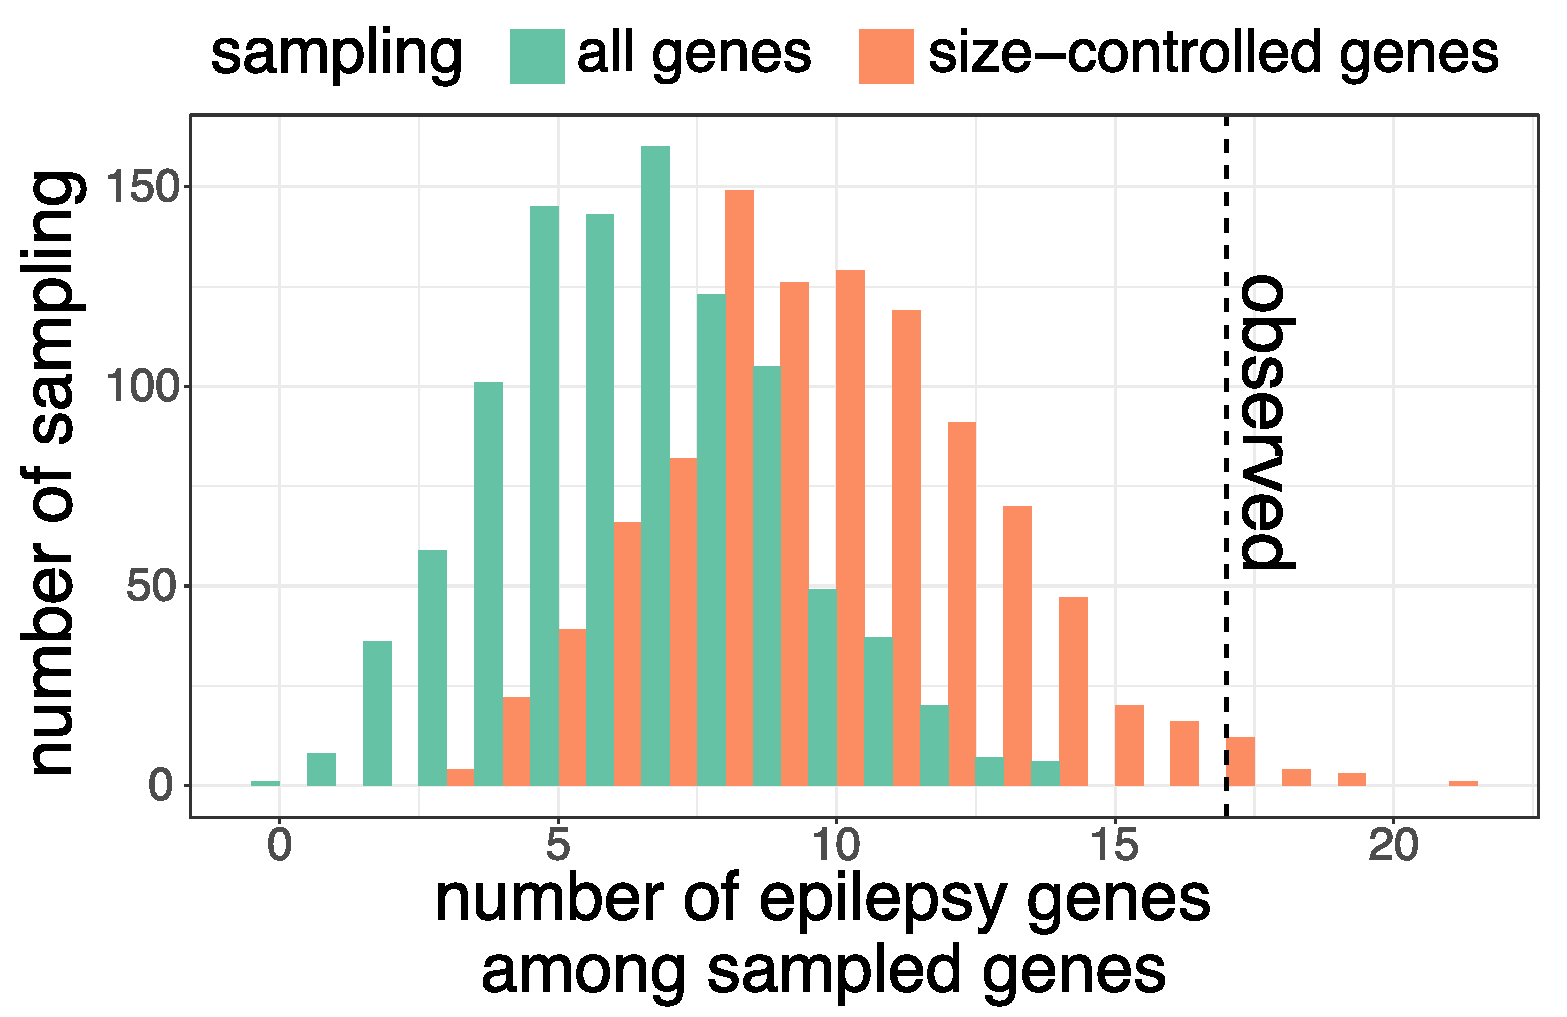
\includegraphics[width=\linewidth,page=1]{figures/epilepsy-enrichmentPatterns-long.pdf}
    \caption{}
    \label{fig:epicnvexex}
  \end{subfigure}
  
  \begin{subfigure}[b]{.9\textwidth}
    \includegraphics[width=\linewidth, page=8]{figures/epilepsy-enrichmentPatterns.pdf}
    \caption{}
    \label{fig:epidistncfun}
  \end{subfigure}
  \caption[CNVs and epilepsy genes.]{{\bf CNVs and epilepsy genes.} {\small a) Number of rare CNVs in or close to exons of protein-coding genes (top) or epilepsy genes (bottom), in the epilepsy cohort. b) Number of epilepsy genes hit by exonic deletions in the epilepsy cohort and never seen in the public and internal databases (dotted line), compared to the expected distribution in all genes and size-matched genes (histograms). c) Rare non-coding CNVs in functional regions near epilepsy genes. The graph shows the cumulative number of individuals (y-axis) with a rare non-coding CNV located at X Kbp or less (x-axis) from the exonic sequence of a known epilepsy gene. We used CNVs overlapping regions functionally associated with the epilepsy gene (eQTL or promoter-associated DNase site).}}
\end{figure}


To get a better idea of the functional regions close to epilepsy genes, we retrieved their associated eQTLs in the GTEx database\cite{Ardlie2015} and the DNase hypersensitivity sites associated with their promoter regions\cite{Maurano2012}.
Notably, focusing on rare non-coding CNVs overlapping these functional regions, the enrichment in epileptic patients was greatly strengthened and clearly present up to 100 Kbp from an epilepsy gene (Kolmogorov-Smirnov test: P-value $9\times10^{-5}$, Fig. \ref{fig:epidistncfun}).
Comparing epilepsy patients and controls, the odds ratio of having such a CNV at a distance of 100 Kbp or less from an exon was 1.33 and gradually increased the closer to the exon (2.9 for CNVs at 5 Kbp or less, Fig. \ref{fig:epidistncfunOR}).
These non-coding CNVs were rare even in the epileptic cohort, but collectively represented an important fraction of affected patients.
While 20 patients (10.1\%) had exonic CNVs in epilepsy genes that were not seen in any control or in the public and internal databases, this number rose to 57 patients (28.8\%) when counting non-coding CNVs in functional regions located at less than 100 Kbp of an epilepsy gene. %71 epilepsy genes were affected across the 92 patients.
These non-coding CNVs were never seen in the controls nor the CNV databases and overlap with annotated enhancer of epilepsy genes.
Although their functional impact remains putative, we believe these CNVs to be of high-interest for the identification of disease causing genes.
Among these CNVs of high-interest, a duplication of a regulatory region 5 Kbp downstream of {\it CSNK1E} was detected and validated in two different patients but absent from our controls and the public and internal databases (Fig. \ref{fig:ncepiex1}).
Another example is a short deletion of an extremely conserved region downstream of {\it FAM63B}, detected in one patient and overlapping expression QTLs for this epilepsy gene (Fig. \ref{fig:ncepiex2}).

\subsection*{Putatively pathogenic CNVs}
Next, we used an array of criteria to select the rare CNVs (less than 1\% in 301 controls) with the highest disruptive potential in the epilepsy cohort.
Priority was given to exonic CNVs in genes already known to be associated with epilepsy.
For CNVs in other genes, we also prioritize recurrent variants and deletions in genes highly intolerant to loss-of-function mutations.
In total, we identified 21 such putative pathogenic CNVs (Tables \ref{tab:1}-\ref{tab:2} and Table \ref{tab:supp}).
Out of these, 8 directly affected a gene previously associated with epilepsy\cite{Ran2015} (Table \ref{tab:1}).
In particular, we identified a deletion resulting in the loss of more than half of the \textit{DEPDC5} gene in a patient affected with partial epilepsy.
A number of point mutations have previously been reported in this gene for the same condition\cite{Dibbens2013,Ishida2013}.
We also identified two deletions and one duplication in \textit{CHD2} gene (see Fig. \ref{fig:popsvCHD2}).
The first deletion is large and affects a major portion of the gene while the second is a small 4.6 Kbp deletion of exon 13, the last exon of {\it CHD2}'s second isoform (Fig. \ref{fig:chd213}).
No exon-disruptive CNVs were reported in any individuals from the control cohort.
This gene was previously associated with patients suffering from photosensitive epilepsy\cite{Galizia2015}.
Interestingly, all three patients carrying the CNVs in \textit{CHD2} have been diagnosed with eyelid myoclonia epilepsy with absence, the same diagnosis that was largely enriched in the Galizia \textit{et al.} study.
Other known epilepsy genes affected by deletions include \textit{LGI1} and the 15q13.3 region.

\begin{figure}[!h]
  \centering
  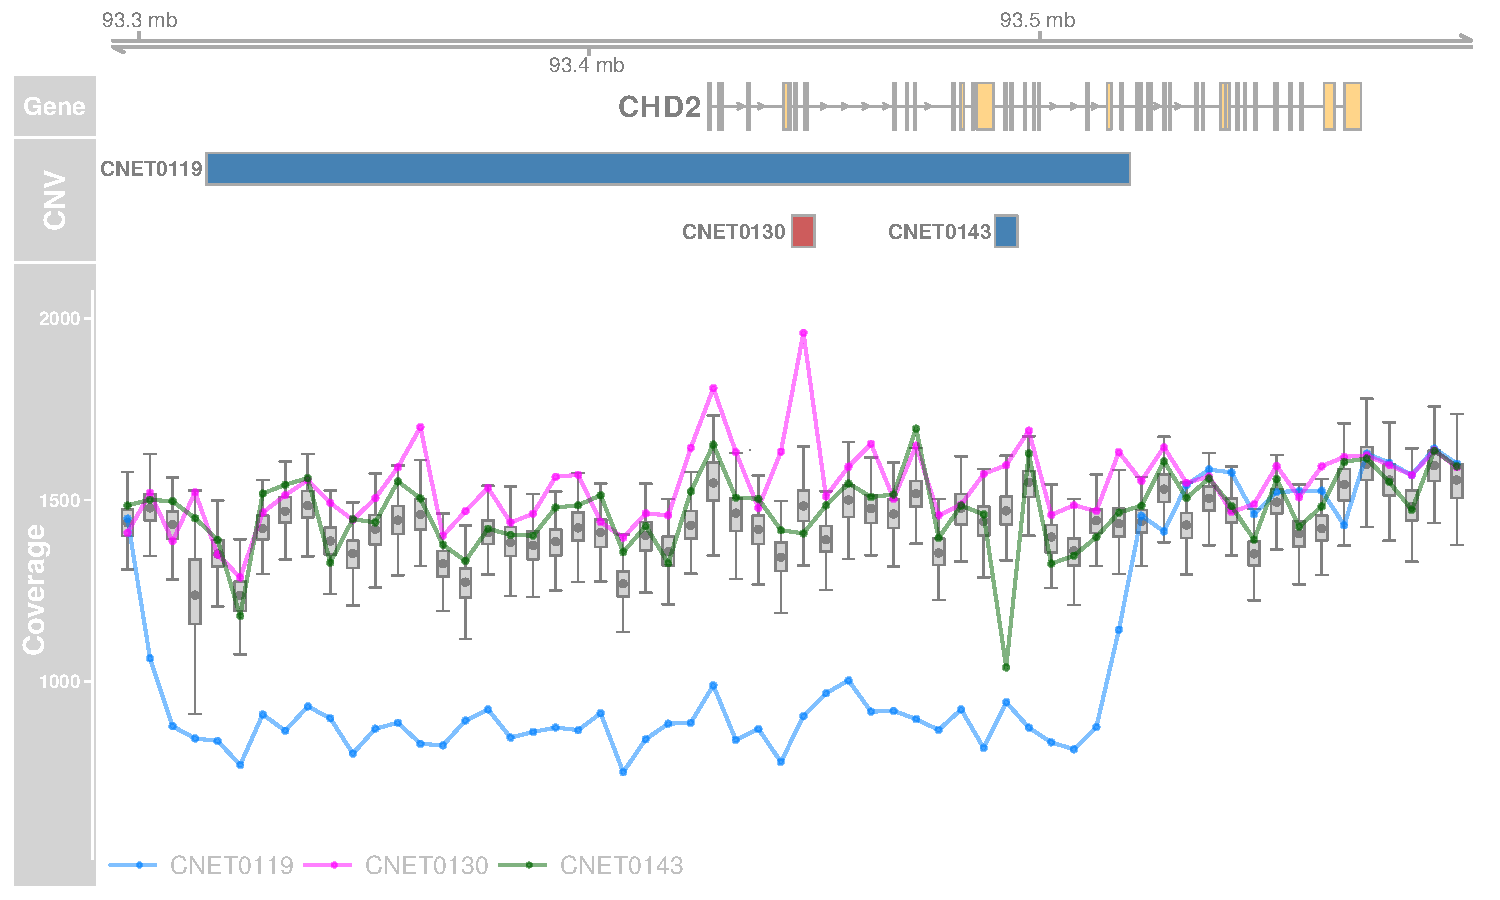
\includegraphics[width=.8\linewidth, page=1]{figures/EpiPopSV-example.pdf}
  \caption[Exonic CNVs in {\it CHD2} detected by {\sf PopSV}.]{{\bf Exonic CNVs in {\it CHD2} detected by {\sf PopSV}.} {\small The 'CNV' panel shows the exonic deletions (blue) and duplications (red) called by {\sf PopSV}. The 'Coverage' panel shows the read depth signal in the affected individuals (colored points/lines) and the coverage distribution in the reference samples (boxplot and grey point).}}
  \label{fig:popsvCHD2}
\end{figure}

\begin{table}[!ht]
  \centering
  \caption[Pathogenic profiles in known epilepsy genes.]{{\bf Pathogenic profiles in known epilepsy genes.}}
  % \begin{tabular}{|l|l|l|r|r|r|p{.2\textwidth}|r|l|l|l|l|l|}
  \resizebox{\textwidth}{!}{
    \begin{tabular}{|l|l|p{.3\textwidth}|l|l|l|l|l|l|l|l|l|l|}
      \hline
      \multirow{2}{*}{{\bf Patient  }} & \multirow{2}{*}{{\bf Epilepsy type }} & \multirow{2}{*}{{\bf Syndrome}} &  {\bf Copy}  & \multirow{2}{*}{{\bf Chr. }} & \multirow{2}{*}{{ \bf CNV start }} & \multirow{2}{*}{{ \bf CNV end   }} & { \bf Epilepsy gene with } & \multirow{2}{*}{{ \bf Taqman probe   }} & \multicolumn{2}{c|}{{\bf Discovery} } & \multicolumn{2}{c|}{{\bf Replication}} \\

                                       &             &                                         & {\bf number} &                     &           &           & {\bf exon disrupted}  &                 & {\bf Patients  } & {\bf Controls } & {\bf Patients     } & {\bf Controls    } \\
      \hline
      CNET0108   & Generalized & Eyelid myoclonia epilepsy with absence  & 1            & 1                   & 44195001  & 44460000  & {\it ST3GAL3}               & Hs05759463\_cn  & 1 DEL            & 0               & 0                   & -                  \\
      \hline
      CNET0159 & Generalized & Eyelid myoclonia epilepsy with absence  & 1            & 8                   & 141925001 & 142010000 & {\it PTK2}                 & Hs06202928\_cn  & 1 DEL            & 0               & 0                   & -                  \\
      \hline
      CNET0093 & Generalized & Juvenile onset; GTCs, Abs, Comp Partial & 1            & 10                  & 95525001  & 95545000  & {\it LGI1}                 & Hs02682696\_cn  & 1 DEL            & 0               & 0                   & -                  \\
      \hline
      CNET0140 & Generalized & Idiopathic generalized epilepsies       & 1            & 13                  & 35750001  & 35785000  & {\it NBEA}                  & Hs05286691\_cn  & 1 DEL            & 0               & 0                   & -                  \\
      \hline
      CNET0144 & Generalized & Eyelid myoclonia epilepsy with absence  & 1            & 15                  & 22745001  & 23275000  & {\it NIPA2}                 & Hs04452887\_cn  & 3 DEL            & 2 DEL           & 4 DEL (2DUP)        & 1 DEL (5 DUP)      \\
      \hline
      CNET0009 & Generalized & Idiopathic generalized epilepsies       & 1            & 15                  & 30910001  & 32445000  & {\it CHRNA7}                & Hs03909657\_cn  & 1 DEL            & 0               & 3 DEL               & (1 DUP)            \\
      \hline
      CNET0119 & Generalized & Eyelid myoclonia epilepsy with absence  & 1            & \multirow{3}{*}{15} & 93300001  & 93515000  & \multirow{3}{*}{{\it CHD2}} & Hs05385106\_cn  & 1 DEL            & 0               & 0                   & -                  \\
      CNET0143 & Generalized & Childhood absence epilepsy              & 1            &                     & 93489776  & 93494317  &                       & Hs026436998\_cn & 1 DEL            & 0               & 0                   & -                  \\
      CNET0130 & Generalized & Eyelid myoclonia epilepsy with absence  & 3            &                     & 93445001  & 93450000  &                       & Hs01379802\_cn  & 1 DUP            & 0               & 0                   & -                  \\
      \hline
      CNET0074 & Focal       & Frontal Lobe  Epilepsy                  & 1            & 22                  & 32125001  & 32255000  & {\it DEPDC5}                & Hs01632214\_cn  & 1 DEL            & 0               & 0                   & -                  \\
      \hline
    \end{tabular}
  }
  \begin{flushleft}
    The 198 epileptic patients and 301 controls represent the discovery set. The replication set contains 325 epileptic patients and 380 controls. Variants that were not tested are marked with ``-''.
  \end{flushleft}
  \label{tab:1}
\end{table}


Four of the 21 putative pathogenic CNVs were found in more than one individual (see Table \ref{tab:2} for precise numbers).
To assess their global prevalence we tested them in an additional cohort of 325 epileptic patients and 380 ethnically matched controls (Table \ref{tab:2}).
Two regions were replicated: the first region in chromosome 2 consists of duplication of the genes \textit{TTC27}, \textit{LTBP1} and \textit{BIRC6}.
In total, 4 patients carried this duplication and it was not reported in any of the two sets of controls.
The second region was found on chromosome 16 and encompasses several genes.
Two deletions were found in epileptic patients for this region and 1 epileptic individual and 1 control were also carriers of a duplication in the same region.
This region corresponds to a genomic hotspot whose deletions were previously associated with epilepsy\cite{Mefford2010} and other neurological disorders.
Finally, the remaining putative pathogenic CNVs were also associated with a number of genes (see Table \ref{tab:supp}).
However, as we lack additional evidence for those specific CNV regions, we propose that these genes should be assessed in independent epilepsy cohorts.
Of note, one patient had a rare 170 Kbp deletion encompassing three exons of the \textit{PTPRD} gene which is predicted to be highly intolerant to loss-of-function mutations (pLI=1)\cite{Lek2016}.
Rare deletions in this gene were previously found in four independent individuals with attention-deficit hyperactivity disorder\cite{Elia2010} and associated with intellectual disability\cite{Choucair2015}.
In addition, {\it de novo} deletions were found in an individual with autism\cite{Pinto2010} and more recently in a patient with epileptic encephalopathy\cite{Mefford2015}.
A common intronic variant in {\it PTPRD} was also associated with remission of seizures after treatment in a clinical cohort of epilepsy patients\cite{Speed2014a}.

\begin{table}[!ht]
  \centering
  \caption[Recurrent CNVs with a pathogenic profile.]{{\bf Recurrent CNVs with a pathogenic profile.}}
  \resizebox{\textwidth}{!}{
    \begin{tabular}{|l|l|p{.3\textwidth}|l|l|l|l|p{.3\textwidth}|l|l|l|l|l|}
      \hline
      \multirow{2}{*}{{\bf Patient}} & \multirow{2}{*}{{\bf Epilepsy type}} & \multirow{2}{*}{{\bf Syndrome }}       & {\bf Copy }  & \multirow{2}{*}{{\bf Chr. }} & \multirow{2}{*}{{\bf CNV start }} & \multirow{2}{*}{{\bf CNV end}} & {\bf Gene with}                                                & \multirow{2}{*}{{\bf Taqman probe }} & \multicolumn{2}{c|}{{\bf Discovery}} & \multicolumn{2}{c|}{{\bf Replication}}                                     \\
                                     &                                      &                                        & {\bf number} &                              &                                   &                                & {\bf exon disrupted}                                           &                                      & {\bf Patients}                       & {\bf Controls}         & {\bf Patients}           & {\bf Controls}         \\
      \hline
      CNET0184                        & Generalized                          & Lennox-Gastaut syndrome                & 3            & \multirow{2}{*}{2}           & \multirow{2}{*}{32625001}         & \multirow{2}{*}{33335000}      & \multirow{2}{*}{{\it TTC27};{\it LTBP1};{\it BIRC6}}                       & \multirow{2}{*}{Hs03387774\_cn}      & \multirow{2}{*}{2 DUP}               & \multirow{2}{*}{0}     & \multirow{2}{*}{2 DUP}   & \multirow{2}{*}{0}     \\
      %% \hline
      CNET0097                        & Generalized                          & Eyelid myoclonia epilepsy with absence & 3            &                              &                                   &                                &                                                                &                                      &                                      &                        &                          &                        \\
      \hline
      CNET0020                        & Generalized                          & Juvenile myoclonic epilepsy            & 1            & \multirow{2}{*}{12}          & \multirow{2}{*}{7995001}          & \multirow{2}{*}{8125000}       & \multirow{2}{*}{{\it SLC2A3};{\it SLC2A14}}                                & \multirow{2}{*}{Hs04406005\_cn}      & \multirow{2}{*}{2 DEL}               & \multirow{2}{*}{2 DEL} & \multirow{2}{*}{2 DEL}   & \multirow{2}{*}{2 DEL} \\
      %% \hline
      CNET0198                        & Focal                                & Frontal lobe epilepsy                  & 1            &                              &                                   &                                &                                                                &                                      &                                      &                        &                          &                        \\
      \hline
      CNET0012                        & Generalized                          & Idiopathic generalized epilepsy        & 3            & \multirow{2}{*}{15}          & \multirow{2}{*}{90845001}         & \multirow{2}{*}{90955000}      & \multirow{2}{*}{{\it ZNF774};{\it IQGAP1}}                                 & \multirow{2}{*}{Hs03895490\_cn}      & \multirow{2}{*}{2 DUP}               & \multirow{2}{*}{0}     & \multirow{2}{*}{(1 DEL)} & \multirow{2}{*}{0}     \\
      %% \hline
      CNET0167                        & Generalized                          & Childhood absence epilepsy             & 3            &                              &                                   &                                &                                                                &                                      &                                      &                        &                          &                        \\
      \hline
      CNET0063                        & Generalized                          & Idiopathic generalized epilepsies      & 3            & \multirow{2}{*}{16}          & \multirow{2}{*}{15460001}         & \multirow{2}{*}{16290000}      & {\it KIAA0430};{\it MPV17L}; {\it NPIPA5};{\it C16orf45}; {\it ABCC6};{\it NDE1}; {\it FOPNL};{\it ABCC1};{\it MYH11} & \multirow{2}{*}{Hs05396556\_cn}      & \multirow{2}{*}{1 DUP + 1 DEL}       & \multirow{2}{*}{0}     & \multirow{2}{*}{1 DEL}   & \multirow{2}{*}{1 DUP} \\
      %% \hline
      CNET0037                        & Generalized                          & Idiopathic generalized epilepsies      & 1            &                              &                                   &                                &                                                                &                                      &                                      &                        &                          &                        \\
      \hline
    \end{tabular}
  }
  \begin{flushleft}
    The 198 epileptic patients and 301 controls represent the discovery set. The replication set contains 325 epileptic patients and 380 controls.
  \end{flushleft}
  \label{tab:2}
\end{table}


\section{Discussion}

Although several tools exist for the detection of CNVs using WGS data, we found that none of them could efficiently account for technical biases, thus resulting in limited sensitivity.
To improve on this, we developed a new tool, {\sf PopSV}, which we demonstrated was able to accurately detect CNVs, including rare and small events.

%% Importance of the reference samples
A key aspect of our approach is the use of a set of reference samples to identify abnormal read coverage.
In this context, the choice and number of reference samples will have an effect on the analysis.
Results from running {\sf PopSV} using different reference cohort sizes suggest that CNV calls are consistent across runs but that a higher number of reference samples increases the sensitivity and robustness of the CNV detection (Fig. \ref{fig:cohortsize}).
Based on these results, we recommend {\sf PopSV} when 20 samples or more can be used as reference.
In a given study, all samples can be used as a reference, or a subset of a few hundreds if the total sample size is extremely large.
Although variants with frequency around 50\% might not be detected, {\sf PopSV} excels at detecting less frequent variants, smaller variants or variants in challenging regions such as repeat-rich regions.
In a case/control design, the control samples could be used as reference in order to maximize the detection of case-specific variants.
In the current study we used both epilepsy patients and controls as reference in order to be able to directly compare the observed CNV distributions.
Finally, in a cancer project with paired normal and tumor samples, only normal samples should be used as reference such that {\sf PopSV} can detect somatic CNVs of any frequency.

%% Importance of same processing. Mention aligner.
To maximize performance, the same library preparation, sequencing and data pre-processing should be employed on all the samples.
To identify potential batch effects, a principal component analysis of read coverage was implemented as part of the {\sf PopSV} package and is recommended to assess the homogeneity of the reference samples.
The read length and aligner can lead to drastic changes in the read coverage and should be consistent across the cohort when analyzed with {\sf PopSV}.
This is particularly important in repeat-rich regions.
Although the different datasets were produced by different sequencing and pre-processing protocols and showed varying degrees of technical bias (Fig. \ref{fig:wgsbias}, \ref{fig:bias:varrank} and \ref{fig:wgsbias2}), the performance of {\sf PopSV} was comparable when benchmarking the methods in the two public datasets and experimentally validating calls in the CENet cohort.

%% Extensions
%% Exome extension
{\sf PopSV}'s approach does not require a uniform read coverage and integrate the coverage variation separately in each studied region.
For these reasons, it would be straightforward to analyze targeted sequencing data, such as exome-sequencing.
%% SV extension
{\sf PopSV} could also be extended for the detection of other types of SVs such as balanced SVs.
To do this, instead of counting properly mapped reads, the method could be modified to test for an excess of discordant reads.
%% Copy-number estimation and breakpoint resolution.
Finally, additional modules could be added to {\sf PopSV} to help characterize the detected variants.
For instance, instead of computing a copy-number estimate from the average coverage in the reference, a HMM approach including all samples could provide a better genotyping strategy.
Similar to other approaches\cite{Abyzov2011,Benjamini2012}, an additional step in the pipeline could explore the effect of the bin size on the variation in read coverage across the population and suggest an optimal bin size.

As in previous array-based studies\cite{Mefford2011,Heinzen2010,Striano2012}, we observed an enrichment of large rare exonic CNVs in patients compared to controls.
However, thanks to the resolution of WGS and {\sf PopSV}, we found that the global distribution of small CNVs ($<$50 Kbp) in 198 unrelated epilepsy patients was also skewed towards rare exonic CNVs.
In addition, genes disrupted by rare deletions in patients were enriched for previously known epilepsy genes.
These observations support the association of small CNVs with epilepsy and could not have been detected in previous array-based studies.

We also observed a clear enrichment of non-coding CNVs in the neighborhood of previously implicated genes.
When focusing on CNVs seen only in the epilepsy cohort and around epilepsy genes, 10.1\% of epilepsy patients have an exonic CNVs and our results shows that up to 28.8\% of patients harbor non-coding CNVs of high-interest in the proximity of epilepsy genes.
These non-coding variants are present in the epilepsy cohort only and located in annotated regulatory regions associated to known epilepsy genes.
Although it is challenging to directly test their functional impact, their frequency and location suggest a putative importance in the genetic mechanism of epilepsy and should be further investigated in the future.

Finally, to better understand the impact of these findings on an individual scale, we selected CNVs with the highest pathogenic potential within our patients.
These CNVs highlighted known but also potentially new epilepsy genes.
Using a second epilepsy cohort, we were also able to identify two chromosomal regions that were recurrently disrupted by CNVs.
These findings highlight the benefits of having a comprehensive survey of CNVs when trying to understand the genetic causes of a disease.


\section{Materials and Methods}

\subsection*{Ethics Statement}
This study was approved by the Research Ethics Board at the Sick Kids Hospital (REB number \verb!1000033784!) and the ethics committee at the Centre Hospitalier Universitaire de Montr\'eal (project number \verb!2003-1394,ND02.058-BSP(CA)!).
Before their inclusion in this study, patients or parents (when needed) had to give written informed consents.

\subsection*{Epilepsy patients and sequencing}
Patients were recruited through two main recruitment sites at the Centre Hospitalier Universitaire de Montr\'eal (CHUM) and the Sick Kids Hospital in Toronto as part of the Canadian Epilepsy Network (CENet).
The main cohort of this study was constituted of 198 unrelated patients with various types of epilepsy; 85 males and 113 females.
The mean age at onset of the disease for our cohort was 9.2 ($\pm$6.7) years.
Table \ref{tab:clinical} presents a detailed description of the clinical features for the various individuals recruited in this study.
301 unrelated healthy parents of other probands from CENet were also included in this study and used as a control cohort.
DNA was exclusively extracted from blood DNA.

Libraries were generated using the TruSeq DNA PCR-Free Library Preparation Kit (Illumina) and paired-end reads of size 125 bp were sequenced on a HiSeq 2500 to an average coverage of 37.6x $\pm$ 5.6x.
Reads were aligned to reference Homo\_sapiens b37 with {\sf BWA}\cite{Li2010}.
Finally, Picard was used to merge, realign and mark duplicate reads.
Raw sequence data has been deposited in the European Genome-phenome Archive, under the accession code \href{https://www.ebi.ac.uk/ega/studies/EGAS00001002825}{EGAS00001002825}.
For more details, see \nameref{sec:suppmat:epipopsv}.

\subsection*{Public WGS datasets}
Two high-coverage public datasets were used to benchmark {\sf PopSV} against existing methods.

A {\it Twin} study provided WGS sequencing data for 45 individuals, including 10 monozygotic twin quartets from the Quebec Study of Newborn Twins\cite{Boivin2013}.
All patients gave informed consent in written form to participate in the Quebec Study of Newborn Twins. Ethic boards from the Centre de Recherche du CHUM, from the Universit\'e Laval and from the Montreal Neurological Institute approved this study.
DNA was extracted from blood and sequencing was done on an Illumina HiSeq 2500 (paired-end mode, fragment length ~300 bp).
The reads were aligned using a modified version of the Burrows-Wheeler Aligner\cite{Li2010} (bwa version 0.6.2-r126-tpx with threading enabled).
The options were \verb!'bwa aln -t 12 -q 5' and 'bwa sampe -t 12'!.
Aligned reads are available on the European Nucleotide Archive under ENA \href{https://www.ebi.ac.uk/ena/data/view/PRJEB8308}{PRJEB8308}.
The 45 samples had an average sequencing depth of 40x (minimum 34x / maximum 57x).

A cancer dataset from a study of renal cell carcinoma\cite{Scelo2014} was also used.
95 pairs of normal/tumor tissues were sequenced using GAIIx and HiSeq2000 instruments.
Paired-end reads of size 100 bp totaled an average sequencing depth of 54x (minimum 26x / maximum 164x).
Reads were trimmed with FASTX-Toolkit and mapped per lane with {\sf BWA}\cite{Li2010} backtrack to the GRCh37 reference genome.
Picard was used to adjust pairs coordinates, flag duplicates and merge lanes.
Finally, realignment was done with {\sf GATK}.
Raw sequence data has been deposited in the European Genome-phenome Archive, under the accession code \href{https://www.ebi.ac.uk/ega/studies/EGAS00001000083}{EGAS00001000083}.
More details can be found in Scelo et al.\cite{Scelo2014}.

\subsection*{Testing for technical biases in WGS}
To investigate the bias in read depth (RD), we fragmented the genome in non-overlapping bins of 5 Kbp and counted the number of properly mapped reads. 
In each sample, we corrected for GC bias and removed bins with extremely low or high coverage (see \nameref{sec:suppmat:epipopsv}). 
Then, read counts across all samples were combined and quantile-normalized. 
Using simulations and permutations, we constructed two control RD datasets with no region-specific or sample-specific bias. 
We computed the mean and standard deviation of the coverage in each bin across samples. 
Next, to investigate experiment-specific bias, we retrieved which sample had the highest coverage in each bin. 
Then we computed, for each sample, the proportion of the genome where it had the highest coverage. 
The same analysis was performed monitoring the lowest coverage. 
This analysis was performed separately on the CENet dataset, the Twin dataset and the normal samples from the cancer dataset.
On the Twin dataset, the same analysis was also run after correcting the read coverage following the {\sf QDNAseq} pipeline\cite{Scheinin2014} (see \nameref{sec:suppmat:epipopsv}).

\subsection*{{\sf PopSV}}
The main idea behind {\sf PopSV} is to assess whether the coverage observed in a given location of the genome diverges significantly from the coverage observed in a set of reference samples.
{\sf PopSV} was implemented in an R package (see \nameref{sec:code}).
The genome is first segmented into bins and the number of reads with proper mapping in each bin is counted for each sample.
In a typical design, the genome is segmented in non-overlapping consecutive windows of equal size, but custom designs could also be used.
With {\sf PopSV}, we propose a new normalization procedure which we call targeted normalization that retrieves, for each bin, other genomic regions with similar profile across the reference samples and uses these bins to normalize read coverage (see \nameref{sec:suppmat:epipopsv}).
Our targeted normalization was compared to global approaches that adjust for the median coverage, or quantile-based approaches.
After normalization, the value observed in each bin is compared with the profiles observed in the reference samples and a Z-score is calculated (Fig. \ref{fig:popsv}).
False Discovery Rate (FDR) is estimated based on these Z-score distributions and a bin is marked as abnormal based on a user-defined FDR threshold.
Consecutive abnormal bins are merged and considered as one variant.
In {\sf PopSV}'s R package, circular binary segmentation\cite{Seshan2017} can also be used to merge bins into variant regions.
Copy number was estimated by dividing the coverage in a region by the average coverage across the reference samples, multiplied by 2 (see \nameref{sec:suppmat:epipopsv}).

\subsection*{Validation and benchmark of {\sf PopSV}}
We compared {\sf PopSV} to {\sf CNVnator}\cite{Abyzov2011}, {\sf FREEC}\cite{Boeva2011} and {\sf cn.MOPS}\cite{Klambauer2012}, three popular RD methods that can be applied to WGS datasets.
We also ran {\sf LUMPY}\cite{Layer2012} which uses an orthogonal mapping signal: the insert size, orientation and split mapping of paired reads. For {\sf LUMPY}, all the CNVs (deletions and duplications) and intra-chromosomal translocations (labeled as 'BND' in Lumpy's output) larger than 300 bp were kept for the upcoming analysis.
These methods were run on the two publicly available datasets, using 5 Kbp bins for the RD methods.

First, we compared the frequency at which a region is affected by a CNV using the calls from the different methods.
To investigate the presence of systematic calls in each method, we compute how many of the calls in a typical sample are called at different frequencies in the dataset.
For example, on average, how many calls in one sample are called in more than 90\% of the samples.
In the Twin dataset, the samples were clustered using the CNV calls from each method.
Different linkage criteria were used for the hierarchical clustering (see \nameref{sec:suppmat:epipopsv}).
The Rand index estimated the concordance between the clustering and the known pedigree (family-level).
Next, we measured the number of CNVs identified in each twin that were also found in their monozygotic twin.
We removed calls present in more than 50\% of the samples to ensure that systematic errors were not biasing our replication estimates.
Hence, a replicated call is most likely true as it is present in a minority of samples but consistently in the twin pair.
For {\sf CNVnator}, {\sf LUMPY} and {\sf PopSV}, the eval1/eval2 columns, number of supporting reads and adjusted P-values (respectively) were used to gradually filter low-quality calls and explore their effect on the replication metrics.
In addition to their replication, we annotated the calls when their region overlapped a call found by other methods in the same sample.
For calls found by at least two methods, we computed the proportion of calls from a method found by each of the other methods.

The approach described previously comparing pairs of twins was also applied in the cancer dataset, on pairs of normal/tumor samples.
In this case, a replicated call is found in the normal sample and in the paired tumor sample.
Finally, we compared calls using small bins (500 bp) and calls using larger bins (5 Kbp).
This comparison explores the quality of the calls, the size of detectable events and the resolution for different bin sizes.
First, we counted how many small bin calls supported any large bin call.
We then looked at the proportion of small bin calls of different sizes that were also found in the large bin calls.

\subsection*{CNV detection in the CENet cohorts}
CNVs were called using {\sf PopSV} using 5 Kbp bins and all the samples from both the epilepsy and control cohorts as reference.
We annotated the frequency of the CNVs using germline CNV calls from the Twin and cancer datasets (internal database) as well as four public CNV databases from the 1000 Genomes Project\cite{Sudmant2015a,Handsaker2015}, the Genome of Netherlands\cite{Francioli2014} and the Simons Genome Diversity Project\cite{Sudmant2015}.
CNVs were annotated with the maximum frequency in the databases.
Hence, a rare CNV is defined as present in less than 1\% of the samples in each of the five CNV databases.

To test for a difference in deletion/duplication ratio among rare CNVs, we compared the numbers of rare deletions and duplications in the epilepsy patients and controls using a $\chi^2$ test.
The same test was performed after downsampling the controls to the sample size of the epilepsy cohort.

\subsection*{Validation by Taqman RT-PCR}
We first selected CNV calls in epilepsy patients that spanned at least 2 consecutive bins.
We kept exonic CNVs of different sizes and overlapping a Taqman probe.
A second batch of CNVs, containing small non-coding CNVs, was also sent for validation.
Here, hundreds of non-coding CNVs spanning only one bin were randomly selected.
When possible the breakpoints were manually fine-tuned from manual inspection of a base-pair level coverage representation or using {\sf IGV}\cite{Thorvaldsdottir2013}; the breakpoints remained unchanged when they could not be refined.
Finally, we kept regions overlapping a Taqman probe.

Probes were selected using the assay search tool on the Thermofisher website.
All probes were tested for patients and controls that were called in {\sf PopSV} as well as an additional 10 control individuals to ensure the validity of the probe.
For each CNV, one assay was chosen in the middle of the genomic region of interest and located in an exon when possible.
All reactions with TaqMan Copy Number Assays were performed in duplex using the FAM dye label based assay for the target of interest (Taqman copy number assay, Made to order, \#4400291, Applied Biosystems by Life Technologies) and the VIC dye label based TaqMan Copy Number Reference Assay for RNase P (4403326, Life technologies).
Amplification reactions ($10\mu L$), which were performed in quadruplicate, consisted of: 10 ng gDNA, 1X TaqMan Copy Number Assay, 1X TaqMan Copy Number Reference Assay, RNase P, 1X TaqMan Genotyping Master Mix (4371355, Life Technologies) or 1X SensiFAST Probe Lo-ROX Kit (BIO-84020, Froggabio).
PCR was performed with an Applied Biosystems QuantStudio7 flex Real-Time PCR system using the standard curve settings and the default universal cycling conditions: 95 $^{\circ}$C 10 minutes followed by 40 cycles: 95 $^{\circ}$C 15 seconds, 60 $^{\circ}$C 60 seconds.
Data was analyzed with QuantStudio Real-Time PCR system software v1.2 (Applied Biosystems by Life Technologies) using autobaseline and manual Ct threshold of 0.2.
Results export files were opened in CopyCaller\textsuperscript{TM} Software v2.0 for sample copy number analysis by the relative quantitation method.
The median $\Delta$Ct was used as the calibrator sample in the analysis settings.

\subsection*{CNV enrichment in exonic regions}
For each cohort (epilepsy and control), we retrieved the CNV catalog by merging CNV that are recurrent in multiple samples.
Hence, the CNV catalog represents all the different CNVs found in each cohort.
Because the epilepsy and control cohorts have different sample sizes, the CNV catalogs for each cohort were built using 150 randomly selected samples.
For each sub-sampling and each cohort, control regions were selected to fit the size distribution of the CNV catalog and the overlap with centromeres, telomeres and assembly gaps (see \nameref{sec:suppmat:epipopsv}).
The fold-enrichment represents how much more/less of the CNVs overlap an exon compared to the control regions.
To robustly compare the two cohorts, we computed the median difference in fold-enrichment between the CNV catalogs from patients and controls across 100 sub-sampled catalogs.
The cohort labels of the CNV catalogs were then permuted 10,000 times and the analysis repeated to derive a null distribution for the median difference in fold enrichment.
A permuted P-value was computed from the observed difference and the null distribution.

Small ($<$50Kbp) and large ($>$50 Kbp) CNVs were analyzed separately.
Exons from genes predicted to be loss-of-function intolerant\cite{Lek2016} (probability of loss-of-function intolerance $>$ 0.9) were also analyzed separately.
The same analysis was repeated using only rare CNVs, i.e. being present in less than 1\% of {\sf PopSV} calls in the Twins and renal cancer datasets, and in four public datasets (see \nameref{sec:suppmat:epipopsv}).

In each cohort, we then retrieved the CNV catalog of rare exonic CNVs.
We evaluated the proportion of the CNVs in the catalog that are private (i.e. seen in only one sample).
The control cohort was down-sampled a thousand times to the same sample size as the epilepsy cohort to provide a confidence interval and empirical P-value (see \nameref{sec:suppmat:epipopsv}).
We also visualize the proportion of CNVs in the catalog seen in 2 samples or more, 3 samples or more, etc (Fig. \ref{fig:epiexpriv}).
We performed the same analysis after removing the top 20 samples with the highest number of non-private rare exonic CNVs.
The analysis was also repeated using French-Canadian individuals only.

\subsection*{CNV enrichment in and near epilepsy genes}
We used the list of genes associated with epilepsy from the EpilepsyGene resource\cite{Ran2015} which consists of 154 genes strongly associated with epilepsy.
We tested different sets of CNVs: deletion or duplications in the epilepsy cohort, control individuals and samples from the twin study, and using different threshold of maximum frequency.
For each set of CNVs, we counted how many of the genes hit were known epilepsy genes.
To control for the size of epilepsy genes and CNV-hit genes, we randomly selected genes with sizes similar to the genes hit by CNVs and evaluated how many were epilepsy genes.
After sampling 10,000 gene sets, we computed an empirical P-value (see \nameref{sec:suppmat:epipopsv}).

To investigate rare non-coding CNVs close to known epilepsy genes, we counted how many patients have such a CNV at different thresholds of distance to the nearest exon.
We compared this cumulative distribution to the control cohort, after down-sampling it to the sample size as the epilepsy cohort.
We performed the same analysis using deletions only.
Each epilepsy gene was also tested for an excess of rare non-coding deletions in patients versus controls using a Fisher test.
Next, we restricted our analysis to rare non-coding CNVs that overlap an eQTL associated with the epilepsy genes\cite{Ardlie2015} or a DNase I hypersensitive site associated with the promoter of epilepsy genes\cite{Maurano2012}.
A Kolmogorov-Smirnov test was used to test the difference in distribution.
Finally, using different values for the maximum distance to the nearest epilepsy gene, we computed the odds ratio of having such a CNV between epilepsy patients and controls.


\subsection*{Putatively pathogenic CNVs}
Exonic CNVs larger than 10 Kbp and found in less than 1\% of the 301 controls were first selected.
We further retained either CNVs overlapping the exon of a known epilepsy-associated gene\cite{Ran2015} or deletions overlapping the exon of a loss-of-function intolerant gene\cite{Lek2016}, or CNVs present in two or more of our epilepsy patients.
All the putatively pathogenic CNVs were validated by Taqman RT-PCR.

\subsection*{Data and code availability}
\label{sec:code}

The {\sf PopSV} R package and its documentation are available at \url{http://jmonlong.github.io/PopSV/}.
Scripts are provided to run the pipeline on different high performance computing systems.
The code used for the analysis and to produce figures and numbers is documented at \url{http://github.com/jmonlong/epipopsv} and archived in \url{https://doi.org/10.5281/zenodo.1172181}.
Necessary data, including the CNV calls, was deposited at \url{https://figshare.com/s/20dfdedcc4718e465185}.
Raw sequence data has been deposited in the European Genome-phenome Archive, under the accession code \href{https://www.ebi.ac.uk/ega/studies/EGAS00001002825}{EGAS00001002825}.

\section{Acknowledgments}
Data analyses were enabled by compute and storage resources provided by Compute Canada and Calcul Qu\'ebec.
We would like to thank Pascale Marquis at the Canadian Centre for Computational Genomics for processing the raw sequencing data to genomic variant calls and for her active participation in various quality assessment steps.
The Canadian Centre for Computational Genomics (C3G) is a Node of the Canadian Genomic Innovation Network and is supported by the Canadian Government through Genome Canada.
We are grateful to the team of the Qu\'ebec Study of Newborn Twins who provided the twin dataset and the Cagekid consortium who provided the renal cancer dataset.
We would like to thank Sylvia Dobrzeniecka for sample handling and lab work.
We are grateful to Dr. Ledia Brunga for her work on the epileptic cohort and to Brianna Goldenstein and Claudia Moreau for revising this manuscript.
Finally, we would like to thank Simon Gravel, Mathieu Blanchette, Mathieu Bourgey, Toby Dylan Hocking and Claudia Moreau for helpful discussions.


%%% Local Variables:
%%% mode: latex
%%% TeX-master: "../main"
%%% End:


\singlespacing
\chapter[Detection of CNVs in Low-Mappability Regions]{Population-Based Detection of CNVs in Low-Mappability Regions}
\label{chap:rep}
\doublespacing
\section*{Preface: Bridging Text between Chapters 3 and 4}
\addcontentsline{toc}{section}{Preface: Bridging Text between Chapters 3 and 4}


The method implemented in the previous chapter was used to study CNVs in low-mappability region.
The main challenge with low-mappability regions is the complex coverage profiles.
Because of the repeated sequences, the number of uniquely mapped reads is reduced and fluctuates depending on which repeats are present in each region.
Instead of attempting to model this complex sequence contexts, we use the population-based approach implemented in chapter \ref{chap:epi}, {\sf PopSV}, to robustly call CNVs in these challenging regions.
Indeed, the complex coverage profiles in low-mappability regions are consistent across samples from the same sequencing project.
Hence, if the read coverage in a sample is different enough from the reference samples, it is likely due to a CNV.

This manuscript was published in {\it Nucleic Acids Research}\cite{Monlong2018nar}.
First, we showed that {\sf PopSV} performance was preserved in low-mappability regions by consistently showing a high sensitivity and a stable false positive rate across different repeat profiles.
Using CNVs across 640 normal genomes we also showed that CNVs are enriched in low-mappability regions independently from the known enrichment in segmental duplication.
Thanks to the population-based approach, we provided a catalog of germline CNV that includes repeat-rich regions, including thousands of regions with recurrent variants that were missing from existing CNV databases.
\nameref{append:rep} contains supplementary tables, graphs and information.

\newpage
\singlespacing

\begin{center}
  \LARGE\bf Human copy number variants are enriched in regions of low mappability
\end{center}
\bigskip

\large{Jean Monlong$^{1,2}$, Patrick Cossette$^{3}$, Caroline Meloche$^3$, Guy Rouleau$^4$, Simon L. Girard$^{1,3,5}$, Guillaume Bourque$^{1,2,6}$}
\bigskip

\footnotesize
$^1$Department of Human Genetics, McGill University, Montr\'eal, H3A 1B1, Canada

$^2$Canadian Center for Computational Genomics, Montr\'eal, H3A 1A4, Canada

$^3$Centre de Recherche du Centre Hospitalier de l'Universit\'e de Montr\'eal, Montr\'eal, H2X 0A9, Quebec, Canada.

$^4$Montreal Neurological Institute, McGill University, Montr\'eal, H3A 2B4, Quebec, Canada.

$^5$D\'epartement des sciences fondamentales, Universit\'e du Qu\'ebec \`a  Chicoutimi, Chicoutimi, G7H 2B1, Canada

$^6$McGill University and G\'enome Qu\'ebec Innovation Center, Montr\'eal, H3A 1A4, Canada

\normalsize
\doublespacing

\section{Abstract}
Copy number variants (CNVs) are known to affect a large portion of the human genome and have been implicated in many diseases.
Although whole-genome sequencing (WGS) can help identify CNVs, most analytical methods suffer from limited sensitivity and specificity, especially in regions of low mappability.
To address this, we use {\sf PopSV}, a CNV caller that relies on multiple samples to control for technical variation.
We demonstrate that our calls are stable across different types of repeat-rich regions and validate the accuracy of our predictions using orthogonal approaches.
Applying {\sf PopSV} to 640 human genomes, we find that low-mappability regions are approximately 5 times more likely to harbor germline CNVs, in stark contrast to the nearly uniform distribution observed for somatic CNVs in 95 cancer genomes.
In addition to known enrichments in segmental duplication and near centromeres and telomeres, we also report that CNVs are enriched in specific types of satellite and in some of the most recent families of transposable elements.
Finally, using this comprehensive approach, we identify 3,455 regions with recurrent CNVs that were missing from existing catalogs.
In particular, we identify 347 genes with a novel exonic CNV in low-mappability regions, including 29 genes previously associated with disease.   


\section{Introduction}

%% Introduce SV/CNV and their importance
Genomic variation of 50 base pairs or more are collectively known as structural variants (SVs) and can take several forms including deletions, duplications, novel insertions, translocations and inversions\cite{Hall2012}.
Copy number variants (CNVs) are unbalanced SVs, i.e. affecting DNA copy number, and include deletions and any type of duplications (tandem duplications, triplications and other amplifications).
A wide range of mechanisms can produce SVs and is responsible for the diverse SV distribution across the genome, both in term of location and size\cite{Hall2012,Sharp2006,Mills2011}.
In healthy individuals, SVs are estimated to cumulatively affect a higher proportion of the genome as compared to single nucleotide polymorphisms (SNPs) \cite{Pang2010}.
SVs have been associated with numerous diseases including Crohn's Disease\cite{McCarroll2008a}, schizophrenia\cite{Stone2008}, obesity\cite{Bochukova2010}, epilepsy\cite{Mefford2011}, autism\cite{Stefansson2014}, cancer\cite{Beroukhim2010} and other inherited diseases \cite{Balzola2010,Ayarpadikannan2014}, and many SVs have a demonstrated detrimental effect. 

%% WGS and its challenges
While large SVs have been first studied using cytogenetic approaches and array-based technologies, whole-genome sequencing (WGS) is in theory capable of detecting SVs of any type and size\cite{Alkan2011}.
Numerous methods have been implemented to detect SVs from WGS data using either paired-end information\cite{Chen2009,Lindberg2014}, read-depth (RD) variation\cite{Boeva2011,Abyzov2011,Klambauer2012}, breakpoints detection through split-read approach\cite{Ye2009} or de novo assembly\cite{Rimmer2014}.
CNVs, potentially the most impactful SVs, can be detected by any of these strategies but are often resolved with a RD approach as it directly looks for signs of copy number changes.
However, several features of WGS experiments result in technical bias and continue to be a major challenge.
For example, GC content\cite{Benjamini2012}, mappability\cite{Treangen2011,Teo2012}, replication timing\cite{Koren2014}, DNA quality and library preparation\cite{VanDijk2014} have a detrimental impact on the uniformity of the RD\cite{Cheung2011}.
Unfortunately, this variability is difficult to fully correct for as it involves different factors, some of which are unknown, that vary from one experiment to another.
This issue particularly impairs the detection of CNV with weaker signal, which is inevitable in regions of low-mappability that represent around 10\% of the human genome\cite{Derrien2012}, for smaller CNVs or in cancer samples with cell heterogeneity or stromal contamination.
As a result, existing approaches suffer from limited sensitivity and specificity\cite{Mills2011,Alkan2011}, especially in regions of low-complexity and low-mappability\cite{Treangen2011,Teo2012}.
Even when problematic regions were masked and state-of-the-art bias correction\cite{Benjamini2012,Scheinin2014} were applied, we showed that technical variation in RD could still be found across three WGS datasets studied\cite{Monlong2018}.

%% Introduce PopSV's approach and compare with other methods
To control for technical variation, we recently developed a CNV detection method, {\sf PopSV}, which uses a set of reference samples to detect abnormal RD\cite{Monlong2018}. 
In each genome tested, the RD in a region is compared to the same region in the reference samples.
{\sf PopSV} differs from most previous RD methods, such as {\sf RDXplorer}\cite{Yoon2009} or {\sf CNVnator}\cite{Abyzov2011}, that scan the genome horizontally and look for regions that diverge from the expected global average.
Even when approaches rely on a ratio between an aberrant sample and a control, such as {\sf FREEC}\cite{Boeva2011} or {\sf BIC-seq}\cite{Xi2011}, we showed that they do not sufficiently control for experiment-specific noise as compared to {\sf PopSV}\cite{Monlong2018}.
Glusman et al.\cite{Glusman2015} does go further and normalize the RD with pre-computed RD profiles that fit the GC-fingerprint of a sample but this approach excludes regions with extreme RD and does not integrate the variance observed in individual regions. % which is essential to robustly deal with mappability bias.
{\sf PopSV} is also different from approaches such as {\sf cn.MOPS}\cite{Klambauer2012} and {\sf Genome STRiP}\cite{Handsaker2015} that scan simultaneously the genome of several samples and fit a Bayesian or Gaussian mixture model in each region.
Those methods have more power to detect CNVs present in several samples but may miss sample-specific events.
Moreover, their basic normalization of the RD and fully parametric models forces them to conceal a sizable portion of the genome and variants with weaker signal.
%% Ensemble approach
Finally, another strategy to improve the accuracy of CNV detection has been to use an ensemble approach that combines information from different methods relying on different types of reads.
Large re-sequencing projects such as the 1000 Genome Project\cite{Sudmant2015a,Mills2011} and the Genomes of Netherlands (GoNL) project \cite{Francioli2014,Kloosterman} have adopted this strategy and have successfully identified many CNVs using an extensive panel of detection methods combined with low-throughput validation.
Such a strategy increases the specificity of the calls at the cost of sensitivity.

Notably, with most of the tools and approaches described above, repeat-rich regions and other problematic regions of the genome are often removed or smoothed at some step of the analysis, to improve the accuracy of the calls. Although some methods\cite{Hormozdiari2010,He2011} try to model ambiguous mapping and repeat structure, only particular situations are addressed and, as a consequence, low-mappability regions are just scarcely covered in the most recent CNV catalogs\cite{Sudmant2015a}. This is unfortunate given that CNVs in such regions have already been associated with various diseases\cite{Ayarpadikannan2014,MacDonald1993,Rich2014,Mirkin2007,Carvalho2016} and that these regions are also more likely variable.
%% Expand on repeats
Indeed, different types of genomic repeats are likely to contribute to CNV formation.
For example, CNVs are known to be enriched in segmental duplications\cite{Sharp2006} and short and long tandem repeats are also known to be highly polymorphic\cite{Gymrek2012,Warburton2008}. Moreover, repeat templates, like segmental duplications or transposable elements, can facilitate the formation of CNV through non-allelic homologous recombination and other mechanisms\cite{Korbel2007}.

%% Outline - What's new since EpiPopSV ?
Given these facts and the growing realization of the importance of repetitive regions in the genome\cite{Hannan2018,Kazazian2017}, we wanted to investigate the performance of {\sf PopSV} in low-mappability regions and explore the comprehensive CNV distribution across a large cohort of healthy individuals.
After showing that population-based RD measures are better than existing mappability estimates to correct for variable coverage, we apply {\sf PopSV} to 640 WGS individuals from three human cohorts.
We compare the performance of {\sf PopSV} on these datasets with existing CNV detection methods in regions of low-mappability and validate the quality of the predictions across different repeat profiles using PCR validation.
Additionally, using publicly available long-read sequencing data and assemblies, we show that {\sf PopSV} is able to detect some highly ambiguous CNVs.
Next, having demonstrated the quality of the {\sf PopSV} calls, we characterize the patterns of CNVs across the human genome and produce a CNV catalog where variants of different types are better represented compared to existing catalogs.
We further find that CNVs are significantly enriched in regions of low-mappability and in different classes of repeats.
Finally, we identify novel CNV regions in low-mappability regions that were absent from previous CNV catalogs and describe their impact on protein-coding genes.

\section{Material and Methods}

\paragraph{Data}
Three publicly available WGS datasets were used.
The first is a twin study\cite{Boivin2013} with an average depth of 40x across 45 French-Canadian individuals, including 10 families of parents and monozygotic twins.
The second is a renal cell carcinoma dataset\cite{Scelo2014} (CageKid) with 95 tumor/normal pairs from four European countries and an average depth of 54x.
The third contains 500 unrelated Dutch individuals from the GoNL\cite{Francioli2014} dataset with an average depth of 14x.
In each study, the sequenced reads had been aligned using {\sf bwa}\cite{Li2010}.
See \nameref{sec:suppmat:reppopsv} for more details on access and read processing.

\paragraph{Read count across the genome}
The genome was fragmented in non-overlapping bins of fixed size.
As a RD measure we used the number of properly mapped reads, defined as read pairs with correct orientation and insert size, and a mapping quality of 30 (Phred score) or more.
In each sample, GC bias was corrected by fitting a LOESS model between the bin's RD and the bin's GC content.
We used a bin size of 5 Kbp for most of the analysis.
When specified, we used smaller bin sizes of 500 bp or 2 Kbp.

\paragraph{RD and mappability estimates}
To compare RD and mappability estimates in the Twin study, we first removed bins with extremely high RD if deviating from the median RD by more than 5 standard deviation.
The RD across the different samples were then combined and quantile normalized.
For each bin, we computed the average RD and standard deviation across the samples.
We downloaded the mappability track for hg19\cite{Derrien2012} and computed the average mappability in each bin.
We compared the RD in one randomly selected sample with the mappability estimates and with the inter-sample RD average.
To correct for the variation explained by the mappability estimates we fitted a generalized additive model using a cubic regression spline between the mappability estimates and RD in the sample (see \nameref{sec:suppmat:reppopsv}).
With these estimations and the global standard deviation we computed a Z-score for each bin.
A similar set of Z-scores was computed using the inter-sample average and standard deviation.
The normality of these two Z-score distributions were compared in term of excess kurtosis and skewness.
The Z-score distributions were also compared in different mappability intervals.
Finally, 45 samples of each cohort were combined and their RD quantile normalized. 
The inter-sample RD mean and standard deviation were then computed separately in each cohort and compared with the mappability estimates and RD in the selected sample.

\paragraph{{\sf PopSV} approach for CNV detection}
{\sf PopSV} was first described and applied in a CNV analysis of epilepsy patients\cite{Monlong2018}.
Briefly, a set of samples are chosen as reference and used to guide the normalization of each bin.
After normalization the average RD and standard deviation in each bin are saved and used to transform the RD in all samples into Z-scores.
CNVs are called in each sample when the RD is significantly higher or lower than in the reference samples.
The Z-scores can be segmented using the circular binary segmentation\cite{Seshan2017} or after statistical testing at the bin level.
As recommended, {\sf PopSV} was run separately on each dataset to avoid false positives due to potential variation in sequencing protocols.
More details are available in the original publication\cite{Monlong2018} and in the \nameref{sec:suppmat:reppopsv}.
With {\sf PopSV} there is no filtering, masking, smoothing or altering of repeat-rich regions: all the regions with properly mapped reads are analyzed.

\paragraph{Coverage track and low-mappability regions}
The average RD in the reference samples, a feature used during CNV calling, was used as a coverage track.
Bins with a RD lower than 4 standard deviation from the median were classified as {\it low-mappability} (or {\it low coverage}).
To highlight the most challenging region, we also defined {\it extremely low coverage} regions if the average RD was lower than 100 reads.
We overlapped these regions with protein-coding genes and segmental duplications (see \nameref{sec:suppmat:reppopsv}), and computed the distance to the nearest centromere, telomere or assembly gap.
We also counted the number of protein-coding genes overlapping at least one low-coverage region.

\paragraph{CNV detection using other methods}
{\sf FREEC}\cite{Boeva2011} and {\sf CNVnator}\cite{Abyzov2011} were run on each sample separately starting from the BAM files and using the same bin size as for {\sf PopSV} (5 Kbp).
{\sf cn.MOPS}\cite{Klambauer2012} was run on the same GC-corrected bin counts than for {\sf PopSV} and samples from the same dataset were jointly analyzed.
After retrieving split reads using {\sf YAHA}\cite{Faust2012}, {\sf LUMPY}\cite{Layer2012} was run and we kept all the deletions and duplications larger than 300 bp.
\verb!BND! variants with both ends more than 300 bp apart in the same chromosome were also included as they could be CNVs lacking support to characterize their type properly.
See \nameref{sec:suppmat:reppopsv} for more details.

\paragraph{Clustering samples using the CNV calls}
The similarity between two samples is defined by the amount of sequence called in both divided by the average amount of sequence called (see \nameref{sec:suppmat:reppopsv}).
This distance is used for hierarchical clustering of the samples in the Twin study using different linkage criteria ({\it average}, {\it complete} and {\it Ward}).
The clustering was performed using calls in regions with extremely low coverage ($\le$100 reads on average in the reference samples) only.
The Rand index estimated the concordance between the clustering and the known pedigree, grouping the samples per family (see \nameref{sec:suppmat:reppopsv}).

\paragraph{Replication in twins}
For each twin and each method, a CNV call was defined as {\it replicated} if also found in the other monozygotic twin but in less than 50\% of the population to remove systematic errors.
The frequency was computed by counting samples with any overlapping CNVs.
In order to avoid missing calls with borderline significance, we used slightly less confident calls for the second twin (see \nameref{sec:suppmat:reppopsv}).
For each method, we computed the number and proportion of {\it replicated} calls per sample.
We computed these metrics using all the calls, calls in low-mappability regions only, calls in segmental duplications, calls overlapping annotated repeats and calls overlapping annotated satellites, all using a minimum overlap of 90\% of the call's sequence.
Finally, we computed the replication estimates for calls located at 1 Mbp or less from a centromere, telomere or assembly gap.

\paragraph{Replication between paired normal and tumor samples}
The same approach was applied in the renal cancer dataset.
Here, {\it replicated} calls were found in a normal sample and its paired tumor but in less than 50\% of the normal samples.

\paragraph{Replication estimates and reliable regions}
Using CNV calls found in less than 50\% of the population, we defined as {\it reliable} a 10 Kbp region where more than 90\% of the overlapping calls were {\it replicated} calls.
We then compared the number and proportion of reliable regions for each method and in different types of region.
As before, we compared regions overlapping low-mappability regions, segmental duplications, annotated repeats, satellites, or located at less than 1Mbp from a centromere, telomere or assembly gap.

\paragraph{Experimental validation}
A subset of variants in the Twin study were experimentally validated.
First, we randomly selected one-copy and two-copy deletions, among small ($\sim700$ bp) and large ($\sim4$ Kbp) variants among the calls produced with 500 bp and 5 Kbp bins.
The calls were visually inspected to design PCR primers (see \nameref{sec:suppmat:reppopsv}).
We randomly selected 20 regions from those with available PCR primers.
Next, we randomly selected deletions overlapping low-mappability regions and called in 6 samples or fewer.
Because RD could not be used efficiently to fine-tune the breakpoints' location, we retrieved the reads (and their pairs) mapping to the region and assembled them (see \nameref{sec:suppmat:reppopsv}).
We randomly selected 17 regions from those with PCR primers.
In addition to gel electrophoresis, the amplified DNA of some regions was sequenced by Sanger sequencing.

\paragraph{Analysis of CEPH12878}
High coverage PCR-free Illumina WGS data for 30 samples, including CEPH12878, was downloaded from the 1000 Genomes Project (1000GP)\cite{Sudmant2015a} (see \nameref{sec:suppmat:reppopsv}).
{\sf PopSV} was run using 5 Kbp bins and all the samples as reference.
Using the same coverage track as before we selected all deletions in CEPH12878 overlapping low-mappability regions (at least 90\% of the call).
We first looked for support in CEPH12878 assemblies that used Illumina short-read sequencing, BioNano Genomics genome maps and either single molecule sequencing from the Pacific Biosciences (PacBio) platform\cite{Pendleton2015} or 10X Genomics linked-read sequencing\cite{Mostovoy2016}.
For each selected deletion from {\sf PopSV}, we aligned the flanking reference sequences to the assemblies using {\sf BLAST}\cite{Camacho2009} (see \nameref{sec:suppmat:reppopsv}).
When both flanks could be mapped to a contig, we visually inspected MUMmer plots\cite{Kurtz2004} which either supported the deletion, the reference genome sequence or were too noisy to assess.
We further annotated the selected calls if they overlapped with the deletions identified in Pendleton et al.\cite{Pendleton2015} over a minimum of 1 Kbp.
Finally, we downloaded the corrected PacBio reads and built a local assembly and consensus around each selected {\sf PopSV} deletion (see \nameref{sec:suppmat:reppopsv}).
We visually inspected MUMmer plots of the assembled and consensus sequences to confirm the presence of the deletion.

\paragraph{CNV catalog}
We called CNVs separately in each cohort with {\sf PopSV} using as reference samples the 45 samples in the Twin study, the normal samples in the cancer dataset and 200 samples in the GoNL dataset.
For the Twin study and the renal cancer dataset, {\sf PopSV} was run using 500 bp bins and 5 Kbp bins.
Because of the lower sequencing depth, {\sf PopSV} was run using 2 Kbp bins and 5 Kbp bins for the GoNL dataset.
For each sample, calls from the 2 different runs were merged when consistent (see \nameref{sec:suppmat:reppopsv}).
To compute the total number of calls, we collapsed calls with a reciprocal overlap higher than 50\%.
The amount of sequence affected in a genome is computed by merging all the variants in the cohort and counting the affected bases in the reference genome.

\paragraph{Comparison with public CNV catalogs}
We retrieved autosomal deletions, duplications and CNVs from four public CNV catalogs derived from large-scale WGS surveys: the 1000GP SV catalog\cite{Sudmant2015a}, {\sf Genome STRiP}'s catalog from 847 individuals\cite{Handsaker2015}, {\sf Genome STRiP} calls in 148 high-depth WGS genomes\cite{Chiang2017}, and the GoNL SV catalog\cite{Francioli2014} (see \nameref{sec:suppmat:reppopsv}).
To compare the amount of CNV with {\sf PopSV}, we removed deletions smaller than 300 bp as well as variants with high frequency ($>80\%$).
We compared CNV frequency between the 620 unrelated samples and a down-sampled set of 620 randomly selected individuals from the 1000GP CNV catalog.
The frequency was derived for all the nucleotide that overlaps at least one CNV as the proportion of individuals with a CNV in this locus.
The frequency distribution was computed separately for the different CNV types.

\paragraph{Comparison with CNV catalogs from long-read studies}
The SV catalog from Chaisson et al.\cite{Chaisson2014} was downloaded and overlapped with the CNV catalogs from 1000GP and {\sf PopSV} results on our 640 genomes.
Here, the 1000GP catalog contained deletions, duplications and CNVs of any size and frequency.
Using control regions and logistic regression we tested for an enrichment of variants in the SV catalog from Chaisson et al.\cite{Chaisson2014} (see \nameref{sec:suppmat:reppopsv}).
The analysis was performed separately on deletions, duplications, low-mappability regions and extremely low-mappability regions.
The same analysis was performed using the SV catalog from Pendleton et al.\cite{Pendleton2015}.

\paragraph{Novel CNV regions}
Using the 620 unrelated individuals across the three cohorts, we selected CNVs present in more than 1\% of the population (7 individuals or more) and not overlapping any CNV in the 1000GP catalog\cite{Sudmant2015a}.
We used deletions, duplications and CNVs of any size and frequency from the 1000GP.
Novel CNVs were collapsed into novel CNV regions, i.e. contiguous regions in which each base is overlapped by at least one novel CNV.
The novel CNV regions were annotated using the low-mappability and extremely low-mappability tracks.
We also compared CNVs from the three other public CNV catalogs to the novel CNV regions.

\paragraph{Distance to centromere, telomere and assembly gaps}
The centromeres, telomeres and assembly gaps (CTGs) were retrieved from the {\sf gap} track in UCSC\cite{Rosenbloom2015}.
In chromosomes with missing telomere annotation, we defined the telomere as the 10 Kbp region at the ends of chromosome.
The distance from each variant to the nearest CTG was computed and represented as a cumulative proportion.
Because this distribution changes with the size of the variants, we sampled random regions in the genome with similar sizes and computed the same distance distribution (see \nameref{sec:suppmat:reppopsv}).
Thanks to this null distribution we were able to see if variants were located closer/further to CTG than expected by chance.

\paragraph{Enrichment in genomic features}
We tested for CNV enrichment in different genomic features: genes, exons, low-mappability regions, segmental duplications, satellites, simple repeats and transposable elements.
The different satellite families, frequent simple repeat motives, transposable element families and sub-families were also tested.
For each sample, we computed a fold-enrichment as the fold change in proportion of regions overlapping a feature between CNV and control regions (see \nameref{sec:suppmat:reppopsv}).
The significance was assessed using logistic regression on the CNV and control regions.
To control for the enrichment in segmental duplications we used control regions with similar overlap profile (see \nameref{sec:suppmat:reppopsv}).
We also added a variable representing the overlap with segmental duplications as a co-factor in the logistic regression model.
When numerous tests were performed, e.g. satellite families, simple repeat motives, transposable element families or sub-families, the P-values were corrected for multiple testing using Benjamini-Hochberg procedure.
Finally, for each CNV and control region, we computed the proportion of the region overlapped by satellites, simple repeats and transposable elements.

\paragraph{Overlap with gene annotation}
Exons of protein-coding genes and promoter regions (10 Kbp upstream of the transcription start site) were extracted from the Gencode annotation v19.
We counted how many genes overlapped a CNV in the population when considering exons only, exons and promoter region, or gene body and promoter region.
In addition, we computed these numbers using only genes associated with a disease or phenotype in the OMIM Morbid Map (Online Mendelian Inheritance in Man; \url{http://omim.org/}).
These numbers were also computed for CNVs that overlapped more than 90\% of various classes of repeats.
For example, Satellite-CNVs are CNVs with more than 90\% of their region annotated as satellites.

\section{Results}

\subsection*{Modeling RD using population-based measures instead of mappability scores}
When counting uniquely mapped reads, the mappability of a region is a major predictor of the observed RD.
Theoretical mappability estimates\cite{Derrien2012} strongly correlated with the RD in a sample but many regions with intermediate mappability diverged from the predicted levels of RD (Fig. \ref{fig:mapcov}).
By computing the average RD across the 45 samples from the Twin study in each 5 Kbp bin we found that this divergence is consistent across samples and not simply due to a high RD variance (Fig. \ref{fig:mapmean}).
\begin{figure}[htp]
  \begin{subfigure}[b]{.48\textwidth}
    \includegraphics[width=\linewidth, page=4]{figures/wgs-map-coverage-cohorts.pdf}
    \caption{}
    \label{fig:mapmean}
  \end{subfigure}
  \begin{subfigure}[b]{.48\textwidth}
    \includegraphics[width=\linewidth, page=5]{figures/wgs-map-coverage-cohorts.pdf}
    \caption{}
    \label{fig:znorm}
  \end{subfigure}

  \begin{subfigure}[b]{.48\textwidth}
    \includegraphics[width=\linewidth, page=6]{figures/wgs-map-coverage-cohorts.pdf}
    \caption{}
    \label{fig:zmap}
  \end{subfigure}
  \begin{subfigure}[b]{.48\textwidth}
    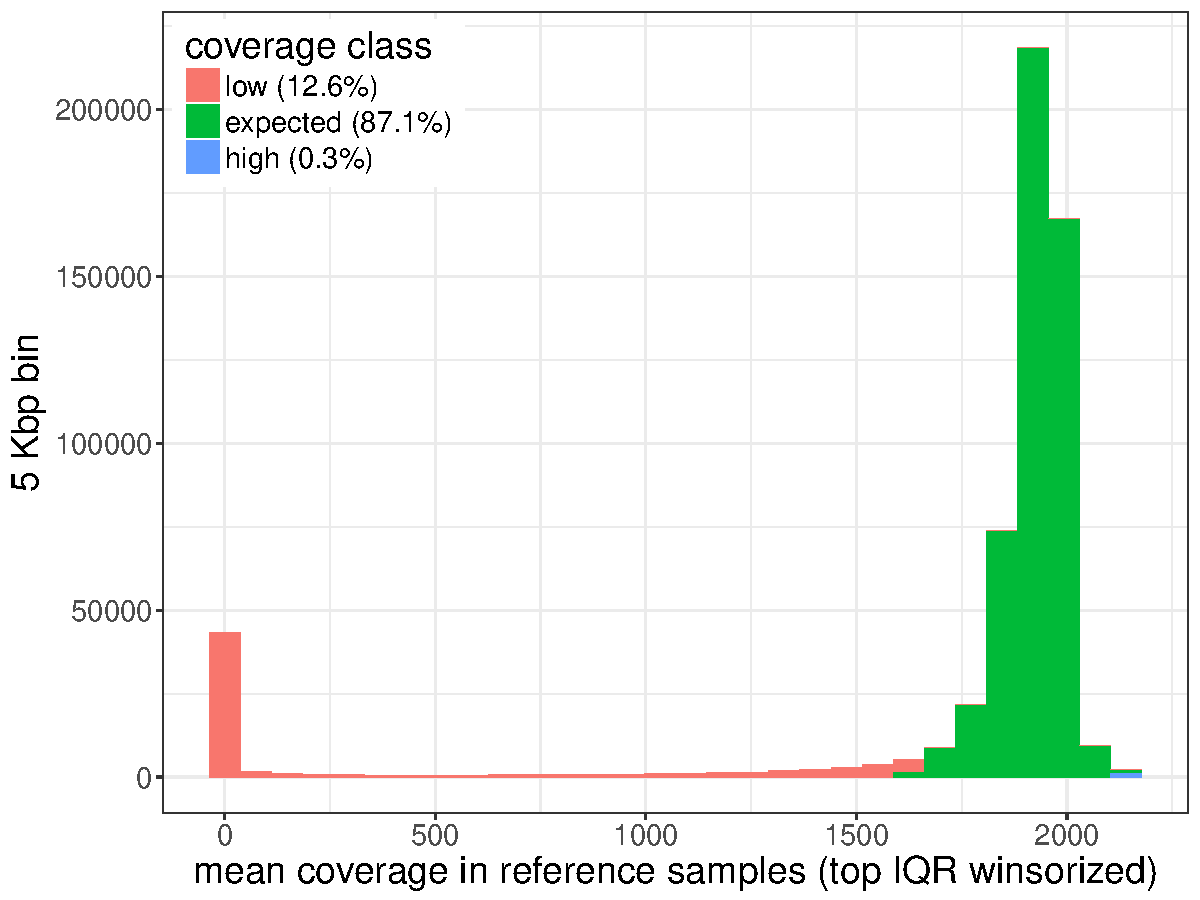
\includegraphics[width=\linewidth, page=1]{figures/wgs-coverage-tracks.pdf}
    \caption{}
    \label{fig:covclass}
  \end{subfigure}

  \caption[Mappability and population-based RD estimates.]{{\bf Mappability and population-based RD estimates.} {\small a) Inter-sample mean RD and average mappability in 5 Kbp bins. Regions with the same mappability estimate can have different RD levels. b) Z-score distribution. In {\it mappability}, Z-scores were computed from the mappability-predicted RD and global standard deviation; In {\it population estimates} from the inter-sample mean and standard deviation. c) Z-score distribution across the mappability spectrum. d) Average RD in the Twin study. The right-tail of the histogram was winsorized using the IQR and the different coverage classes are shown with colors.}}

\end{figure}
These mappability estimates only approximate RD variation and cannot explain the RD profile in numerous regions.
In contrast, population-based metrics more directly estimate the expected RD level (Fig. \ref{fig:meancov}).
Similarly to what was done in Monlong et al. in high-mappability regions\cite{Monlong2018}, we hypothesized that population-based estimates of RD mean and standard deviation could be used directly and help analyze regions with reduced RD.
To test this hypothesis, Z-scores corrected by the mappability-based estimates were compared to Z-scores derived from both the inter-sample mean and standard deviation.
The population-based Z-scores better followed a Normal distribution with an excess kurtosis of 0.2 and skewness of 0.004 compared to 29.4 and -2.284 respectively for mappability-adjusted Z-scores (Fig. \ref{fig:znorm}).
The distribution of the population-based Z-scores was also more stable across the mappability spectrum (Fig. \ref{fig:zmap}).
When comparing samples from the three different datasets, we noticed cohort-specific profiles in term of RD level and variance even though RD had been quantile normalized (Fig. \ref{fig:meancohort} and \ref{fig:sdcohort}), suggesting that population-based estimates will be better at capturing subtle cohort-specific variation.


These results suggest that a population-based strategy such as {\sf PopSV}\cite{Monlong2018} could be extended to investigate CNVs in regions of low-mappability.
To define low-mappability regions in the population, we used the average RD in the reference samples track produced by {\sf PopSV}.
In the Twin study for example, 12.6\% of the covered 5 Kbp bins were labeled as low-coverage (Fig. \ref{fig:covclass}), more than half of which were regions with extremely low coverage (lower than 100 reads on average).
Slightly fewer regions were labeled as low-coverage in the other cohorts (Fig. \ref{fig:covclass2}). As expected, low-coverage regions were depleted in gene content with only 15.3\% of the 5 Kbp bins in these regions overlapping a protein-coding gene versus 48.8\% for other regions. Nonetheless, 4,044 protein-coding genes overlapped a low-coverage region.
Finally, 23.2\% of the low-mappability regions overlapped segmental duplications and 69.1\% were located at less than 1 Mbp from a centromere, telomere or assembly gap, versus respectively 2.9\% and 8.8\% for other regions.

\subsection*{Replication rates in regions of low-mappability}
We previously demonstrated that CNV detection with {\sf PopSV} was overall more sensitive than {\sf FREEC}\cite{Boeva2011}, {\sf CNVnator}\cite{Abyzov2011}, {\sf cn.MOPS}\cite{Klambauer2012} and {\sf LUMPY}\cite{Layer2012} methods\cite{Monlong2018}.
In the following, we focused on the performance of {\sf PopSV} in low-mappability regions.
We first investigated the general concordance of the CNV calls with the pedigree in the Twin study.
Using calls in extremely low-mappability regions (average RD below 100 reads) only, we clustered the individuals and compared the result to the known pedigree.
We found that {\sf PopSV} showed better concordance, as assessed by the Rand index (Fig. \ref{fig:randindex}), compared to the other methods.
Indeed, the clustering dendogram from {\sf PopSV} calls, even in these challenging regions, captured almost perfectly the family relationships (Fig. \ref{fig:cluster}).
\begin{figure}[htp]
  \centering
  \begin{subfigure}[b]{\textwidth}
    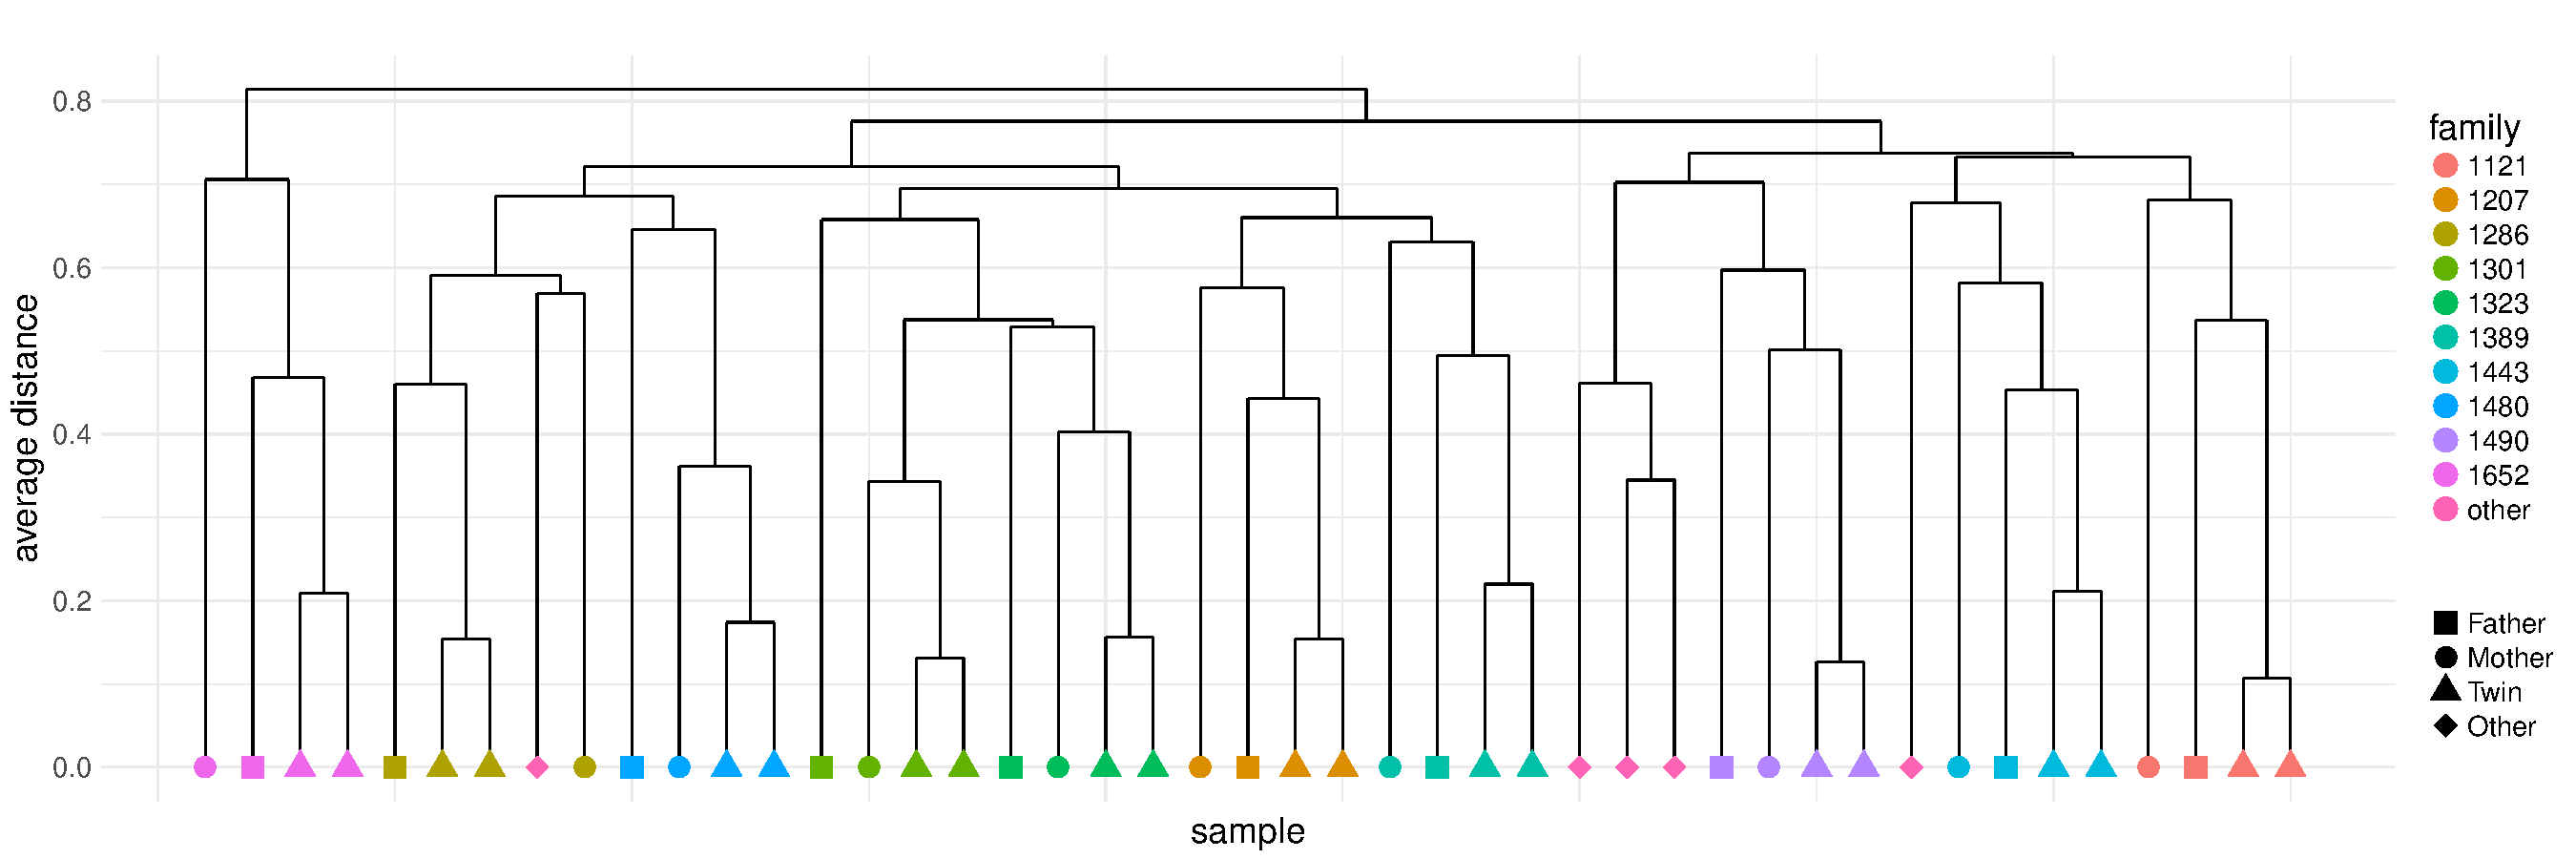
\includegraphics[width=\linewidth]{figures/replication-twins-long.pdf}
    \caption{}
    \label{fig:cluster}
  \end{subfigure}
  
  \begin{subfigure}[b]{.48\textwidth}
    \includegraphics[width=\linewidth, page=2]{figures/replication-twins.pdf}
    \caption{}
    \label{fig:replication}
  \end{subfigure}
  \begin{subfigure}[b]{.48\textwidth}
    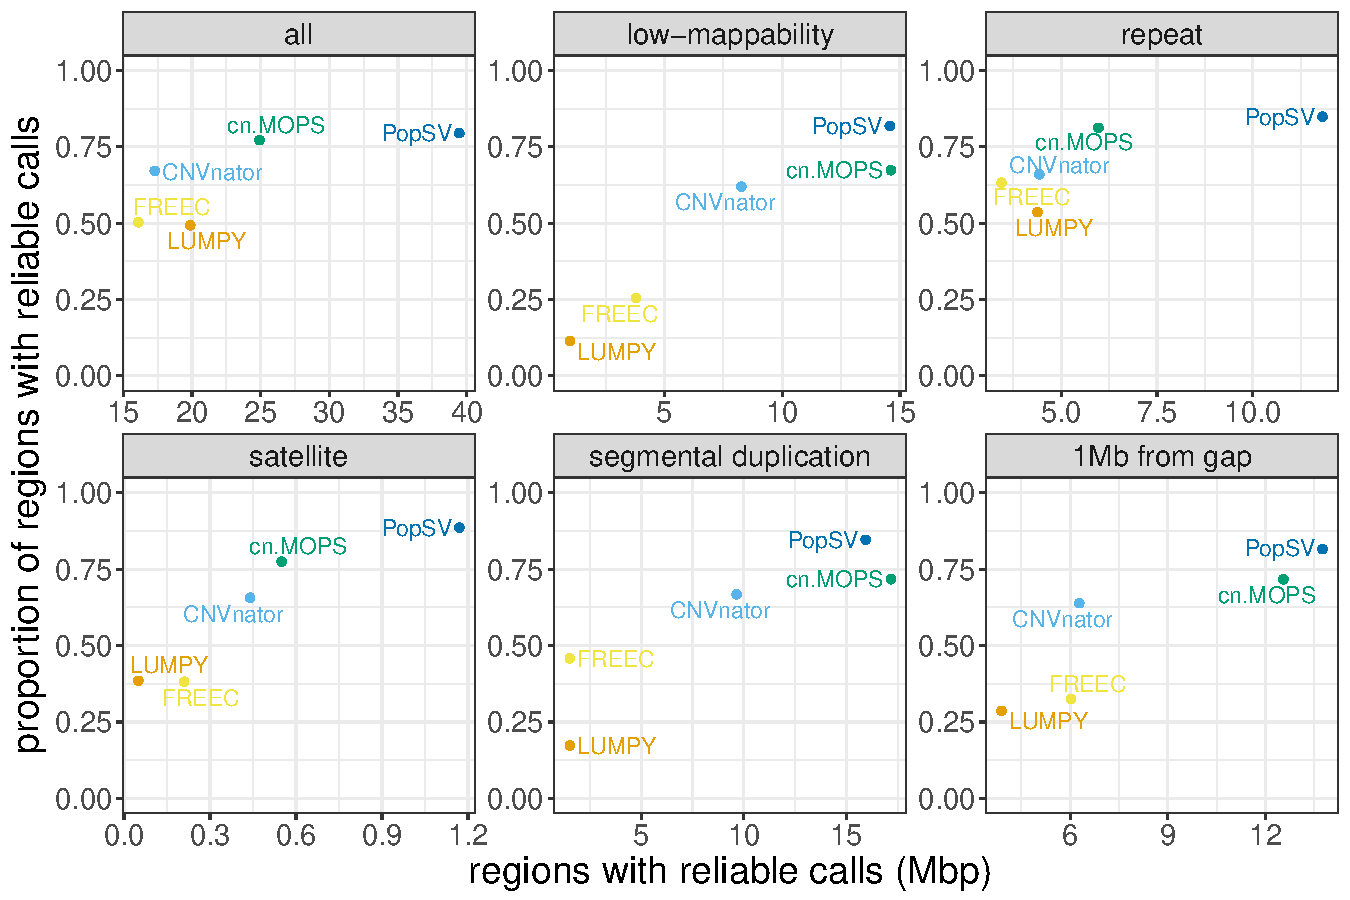
\includegraphics[width=\linewidth, page=1]{figures/replication-twins-reliable.pdf}
    \caption{}
    \label{fig:reliable}
  \end{subfigure}

  \caption[{\sf PopSV}'s performance in low-mappability regions.]{{\bf {\sf PopSV}'s performance in low-mappability regions.} {\small a) Cluster using {\sf PopSV} calls in extremely low coverage regions (below 100 reads). b) Proportion and number of calls replicated in the monozygotic twin. The point shows the median value per sample, the error bars the 95\% confidence interval. c) Proportion and number of regions with reliable calls, computed from call replication in twins.}}
\end{figure}
We then investigated if the call replication rate was stable across different mappability profiles.
Using calls present in less than 50\% of the population to avoid systematic bias, the overall replication rate in the other twin was found to be 89.7\%.
Focusing on calls in low-coverage regions, we found a comparable replication rate of 92.5\%.
The replication rate remained constant in regions with different repeat profiles (Fig. \ref{fig:replication}) such as regions overlapping segmental duplication, annotated repeats, or close to centromeres, telomeres and assembly gaps.
In contrast, the other methods showed a reduced replication and higher variance in repeat-rich regions.
The superior replication rate was complemented by a larger number of calls: {\sf PopSV} called between 2.7 and 9.9 times more replicated CNVs per sample in low-coverage regions compared to the other methods.
We observed the same results in the cancer dataset when comparing the agreement between germline events in normal/tumor pairs.
{\sf PopSV} had between 1.8 and 17.8 times more calls in low-mappability regions compared to the other methods and a stable replication rate across repeat profiles (Fig. \ref{fig:replication:cagekid}).
We next wanted to assess the performance in each region of the genome, rather than overall rates per sample, and used the replication in twins to identify regions with reliable calls.
Again we observed that {\sf PopSV} was as reliable overall as in regions with different repeat profiles (Fig. \ref{fig:reliable}).
This analysis also showed that {\sf PopSV} provides reliable calls in a larger fraction of the genome compared to other methods.
The strongest gain was observed for regions overlapping satellites or overlapping almost completely annotated repeats, with around twice as many regions reliably called by {\sf PopSV}.
{\sf cn.MOPS} showed the second best performance, especially in regions overlapping segmental duplications or close to centromeres, telomeres and assembly gap.

\subsection*{Validation of CNVs in regions of low-mappability}

% \paragraph{Experimental validation}
Using Real-Time PCR validation across 151 regions, we previously demonstrated that the replication estimates from the Twin dataset are consistent with experimental validation\cite{Monlong2018}.
We had tested variants of different types, sizes and frequencies and validated 90.7\% of the calls, similar to our twin-based replication estimates.
Here we tested additional deletions in individuals from the Twin study using PCR validation.
We first validated randomly selected deletions and found a validation rate close to the overall replication rate, with 18 out of 20 deletions (90\%) successfully validated (Table \ref{tab:pcr}).
In a second validation batch, we focused on rare deletions in low-mappability regions, of which 11 out of the 17 (65\%) were successfully validated (Table \ref{tab:pcr2}).
We noticed that the majority of the non-validated deletions were predicted to be smaller than 100 bp and most likely due to a problem during the breakpoint fine-tuning.
If we consider only deletions larger than 100 bp, the validation rate in regions of low-mappability increased to 83\% (10/12) once again close to {\sf PopSV}'s replication rates in the Twin dataset.

Regions with extreme repeat content remained difficult to target and validate using PCR approaches.
To further interrogate the performance of {\sf PopSV} in those regions, we turned to whole-genome data from long-read sequencing technology.
Publicly available assemblies for CEPH12878 samples confirmed several deletions called by {\sf PopSV} in low-mappability regions.
Out of the 14 homozygous deletions that could be assessed, 13 were confirmed in a contig, 12 of which were observed in both assemblies\cite{Pendleton2015,Mostovoy2016}.
Only one region seemed to be a false positive, an assembled contig supporting the reference sequence in one assembly.
Eleven regions could not be assessed because the flanks in the reference genome didn't map to any assembled contigs or their MUMmer plots neither supported a deletion nor the reference sequence.
In summary, we confirmed 92.8\% of the homozygous deletions in low-mappability regions that could be compared with the assemblies.
Deletions can be confirmed by direct comparison of the variant region and, if homozygous, should be present in the assembly.
In contrast, heterozygous deletions could be missing from an assembly if only the reference allele was assembled.
We confirmed 27 out of the 44 heterozygous deletions in low-mappability regions that could be assessed (Table \ref{tab:cephAss}).
As expected, only one allele was supported for many regions: 16 regions with only the deleted allele observed and 17 regions with only the reference allele observed.
Both deleted and reference alleles were observed for 11 variants.
Although only 61.3\% of the heterozygous deletion were confirmed, many variants might have been missed because of assembly preference to one allele, as suggested by the similar number of regions with only one supported allele.
Using variants identified by Pendleton et al.\cite{Pendleton2015} and by assembling raw PacBio reads, we found support for 3 additional homozygous deletions and 15 heterozygous deletions that had remained inconclusive in the assembly comparison.
Most of the regions that couldn't be confirmed were located close to assembly gaps in the reference genome (Fig. \ref{fig:cephGap}).
This observation highlighted that even with long-read sequencing data, it is not straightforward to clearly assess some genomic regions close to assembly gaps.

\subsection*{Global patterns of CNVs across the human genome}

Having demonstrated the robustness of {\sf PopSV} in low-mappability regions, we wanted to characterize the global patterns of CNVs across the human genome.
We were especially interested in looking at calls in regions of low-mappability which represents between 9-12\% of the human genome (Fig. \ref{fig:covclass} and \ref{fig:covclass2}).
We started with an analysis of the twins and the normal samples in the renal cancer dataset, both of which have an average sequencing depth around 40X.
{\sf PopSV} was used to call CNV using 500 bp and 5 Kbp bins, which were then merged to create a final set of variants.
On average per genome, 7.4 Mbp of the reference genome had abnormal read coverage, 4 Mbp showing an excess of reads indicating duplications and 3.4 Mbp showing a lack of reads indicating deletions (Table \ref{tab:res}).
\begin{sidewaystable}
  \resizebox{\textwidth}{!}{
    \begin{tabular}{|l|r|r|rrr|r|rr|rrrr|}
      \hline
      \multirow{2}{*}{Set}  & \multirow{2}{*}{Depth} & \multirow{2}{*}{Samples} & \multicolumn{3}{c|}{Variants} & \multirow{2}{*}{Avg Size (Kbp)} & \multicolumn{2}{c|}{Variants $<$3 Kbp} & \multicolumn{4}{c|}{Affected genome (Mbp)}                                       \\
                            &                        &                          & Total                         & \multicolumn{2}{c|}{Per sample} &                                        & Proportion & Per sample & Total   & \multicolumn{3}{c|}{Per sample}             \\
      \hline
                            &                        &                          &                               & {\it WG}                        & {\it ELC}                               &            &            &         &        & {\it min} & {\it mean} & {\it max} \\
                            % \hline


      Twin study            & 42x & 45  & 20,222 & 1,637.27 & 243.24 & 4.21 & 0.65 & 1,056.84 & 62.22  & 5.30 & 6.89 & 9.03  \\
      {\it ~~deletion}      &     &     & 10,661 & 727.04  & 13.20  & 4.53 & 0.58 & 423.80  & 33.97  & 2.79 & 3.30 & 3.85  \\
      {\it ~~duplication}   &     &     & 10,396 & 910.22  & 230.04 & 3.94 & 0.70 & 633.04  & 34.20  & 2.50 & 3.59 & 5.29  \\
      \hline                                                                                                                                                                  
      CageKid normals & 40x & 95  & 56,256 & 2,132.81 & 336.46 & 3.58 & 0.71 & 1,521.16 & 134.77 & 5.53 & 7.63 & 10.24 \\
      {\it ~~deletion}      &     &     & 25,367 & 805.08  & 12.74  & 4.30 & 0.63 & 508.56  & 70.65  & 2.65 & 3.46 & 7.26  \\
      {\it ~~duplication}   &     &     & 32,356 & 1,327.73 & 323.73 & 3.14 & 0.76 & 1,012.60 & 76.28  & 2.31 & 4.17 & 6.70  \\
      \hline                                                                                                                                                                  
      GoNL                  & 13x & 500 & 27,945 & 549.52  & 81.97  & 8.71 & 0.46 & 250.24  & 226.50 & 3.05 & 4.79 & 8.16  \\
      {\it ~~deletion}      &     &     & 13,818 & 262.41  & 1.45   & 8.50 & 0.42 & 110.16  & 106.83 & 1.30 & 2.23 & 3.96  \\
      {\it ~~duplication}   &     &     & 15,291 & 287.10  & 80.52  & 8.91 & 0.49 & 140.08  & 139.21 & 1.45 & 2.56 & 5.72  \\
      \hline
    \end{tabular}
  }
  \caption[CNVs in the Twins, CageKid normals and GoNL datasets.]{{\bf CNVs in the Twins, CageKid normals and GoNL datasets. }{\small WG: whole genome; ELC: extremely low-coverage regions. The {\it Total} number of variants is the total number after collapsing recurrent variants. {\it Affected genome} represents the amount of the reference genome that overlaps at least one CNV.}}
  \label{tab:res}
\end{sidewaystable}
In both datasets, the average variant size was around 3.7 Kbp and 70\% of the variants found were smaller than 3 Kbp.
We compared our numbers to equivalent CNVs detected in the most recent human SV catalog from the 1000 Genomes Project (1000GP), where 6.1 Mbp was found to be copy-number variable on average in each genome (Table \ref{tab:1kgp}).
In those calls, we notice that no variants except for a few deletions were identified in regions of extremely low-mappability regions.
Similarly, small duplications ($<3$ Kbp) were absent from that catalog.
In contrast, the set of variants identified by {\sf PopSV} included variants in extremely low-mappability regions as well as small deletions and duplications (Table \ref{tab:res}), explaining in part the $\sim20\%$ increase in affected genome.
While the study from the 1000GP\cite{Sudmant2015a} explored a wider range of SVs, our catalog is likely more representative of the distribution of CNVs in a normal genome since a larger portion of the genome could be analyzed.
Small duplications and events in low-mappability regions were also under-represented in more recent CNV surveys that used higher sequencing depth or joint-calling of CNVs\cite{Handsaker2015,Chiang2017,Francioli2014} (Table \ref{tab:1kgp}), confirming the uniqueness of the PopSV catalog.

Next, we applied {\sf PopSV} to the 500 unrelated samples from the GoNL cohort (Table \ref{tab:res}).
Due to a lower sequencing depth ($\sim$13X), we used bins of size 2 Kbp and 5Kbp, explaining the lower number of variants found in these samples.
Nevertheless, a large sample size helps better characterize the frequency patterns and provides a more comprehensive map of rare CNVs.
In total, across these three cohorts, 325.6 Mbp were found to be affected by a CNV with more duplications (50,856) detected than deletions (44,110).
This contrasts with the CNVs reported by the 1000GP\cite{Sudmant2015a} that were heavily skewed towards deletions (Table \ref{tab:1kgp}), likely due to the conservative ensemble approached used to detect CNVs.
The frequency distribution of deletions and duplications found using {\sf PopSV} were also much more balanced compared with the ones from the 1000GP\cite{Sudmant2015a} (Fig. \ref{fig:freq1kgp}).
\begin{figure}[htp]
  \centering
  \begin{subfigure}{.49\textwidth}
    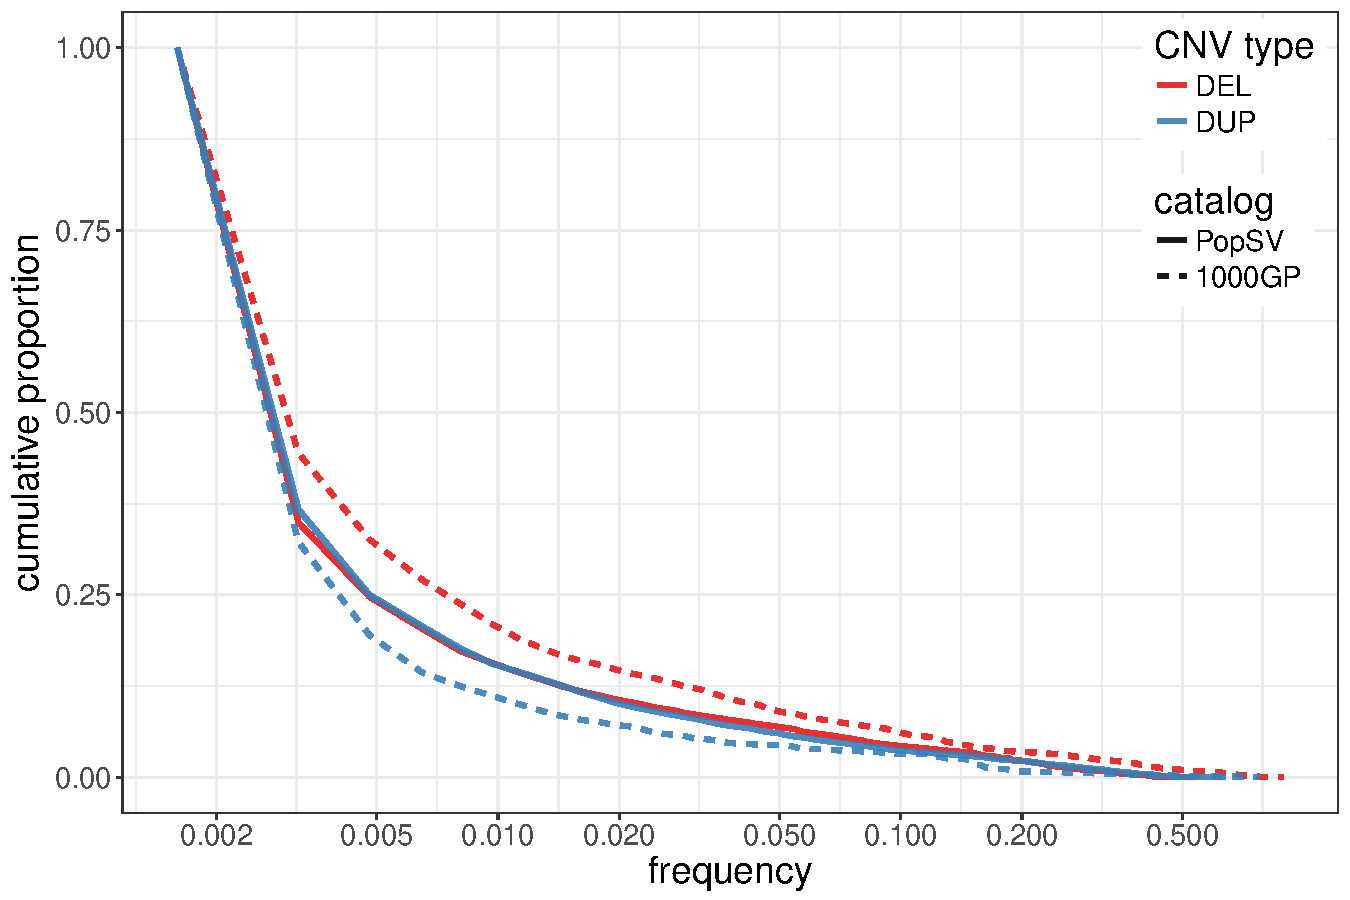
\includegraphics[width=\linewidth,page=1]{figures/PopSV-catalog-overview.pdf}
    \caption{}
    \label{fig:freq1kgp}
  \end{subfigure}
  \begin{subfigure}{.49\textwidth}
    \includegraphics[width=\linewidth,page=2]{figures/PopSV-catalog-overview.pdf}
    \caption{}
    \label{fig:chaisson}
  \end{subfigure}
  \caption[Comparison with CNV catalogs from the 1000 Genomes Project and a long-read sequencing study]{{\bf Comparison with CNV catalogs from the 1000 Genomes Project\cite{Sudmant2015a} (1000GP) and a long-read sequencing study\cite{Chaisson2014}.} {\small a) The x-axis represents the proportion of individuals with a CNV overlapping a region. The y-axis represents the cumulative proportion of the affected genome. b) Overlap with the SV catalog from Chaisson et al.\cite{Chaisson2014}. In each cohort (color), the proportion of collapsed calls overlapping calls from Chaisson et al.\cite{Chaisson2014} or control regions with similar size distribution was modeled using a logistic regression. Boxplots show variation across 50 sampling of control regions. {\it low-map}: calls in low-mappability regions; {\it ext. low-map}: calls in extremely low-mappability regions.}}
\end{figure}
We also compared our CNV catalog with an orthogonal set of calls from Chaisson et al.\cite{Chaisson2014} that were obtained using long-read sequencing.
Although these calls came from a different genome, we expect both catalogs to share a number of common variants.
We found a significant overlap between the two catalogs, overall and separately for deletions, duplications, low-mappability regions and extremely low-mappability regions (Fig \ref{fig:chaisson}).
In all categories, the overlap was stronger for {\sf PopSV}'s catalog compared to the 1000GP CNV catalog.
We noted that the enrichment for the 1000GP catalog disappeared for duplications and low-mappability regions but was even stronger for {\sf PopSV}'s catalog.
Like {\sf PopSV}, the long-read sequencing study\cite{Chaisson2014} also found a better balance between deletions and duplications.
Similar observations were made using another set of calls from long-read sequencing of the CEPH12878 sample\cite{Pendleton2015} (Fig. \ref{fig:pendcat}).

\subsection*{CNVs are enriched near centromeres and telomeres and in regions of low-mappability}

Large CNVs have been shown to be enriched near centromeres, telomeres and assembly gaps (CTGs)\cite{Nguyen2006}.
We were interested in exploring this observation further using the set of high resolution calls from {\sf PopSV}.
We compared the distribution of CNVs calls made across the 3 datasets to randomly distributed regions of similar sizes (Fig. \ref{fig:ctgDist}).
In an average genome, we found that 33.5\% of the CNVs calls were within 1 Mbp of a CTG, while we would have expected only 11.2\% by chance.
To verify that these observations were not simply a consequence of the methodology used, we also looked at the somatic CNVs (sCNVs) that we could detect in the renal cell carcinoma dataset.
For this purpose, we extracted the variants found by {\sf PopSV} in the tumor sample of an individual but missing from its paired normal sample.
Reassuringly, and in contrast to germline CNVs, sCNVs were not preferentially found near CTGs (Fig. \ref{fig:ctgDist}), with 11.1\% of the sCNVs within 1 Mbp of a CTG.

After correcting for the distance to CTGs, we also observed a 4.7 fold-enrichment of variants in regions of low mappability (Fig. \ref{fig:repAll}).
\begin{figure}[htp]
  \centering
  \begin{subfigure}{.9\textwidth}
  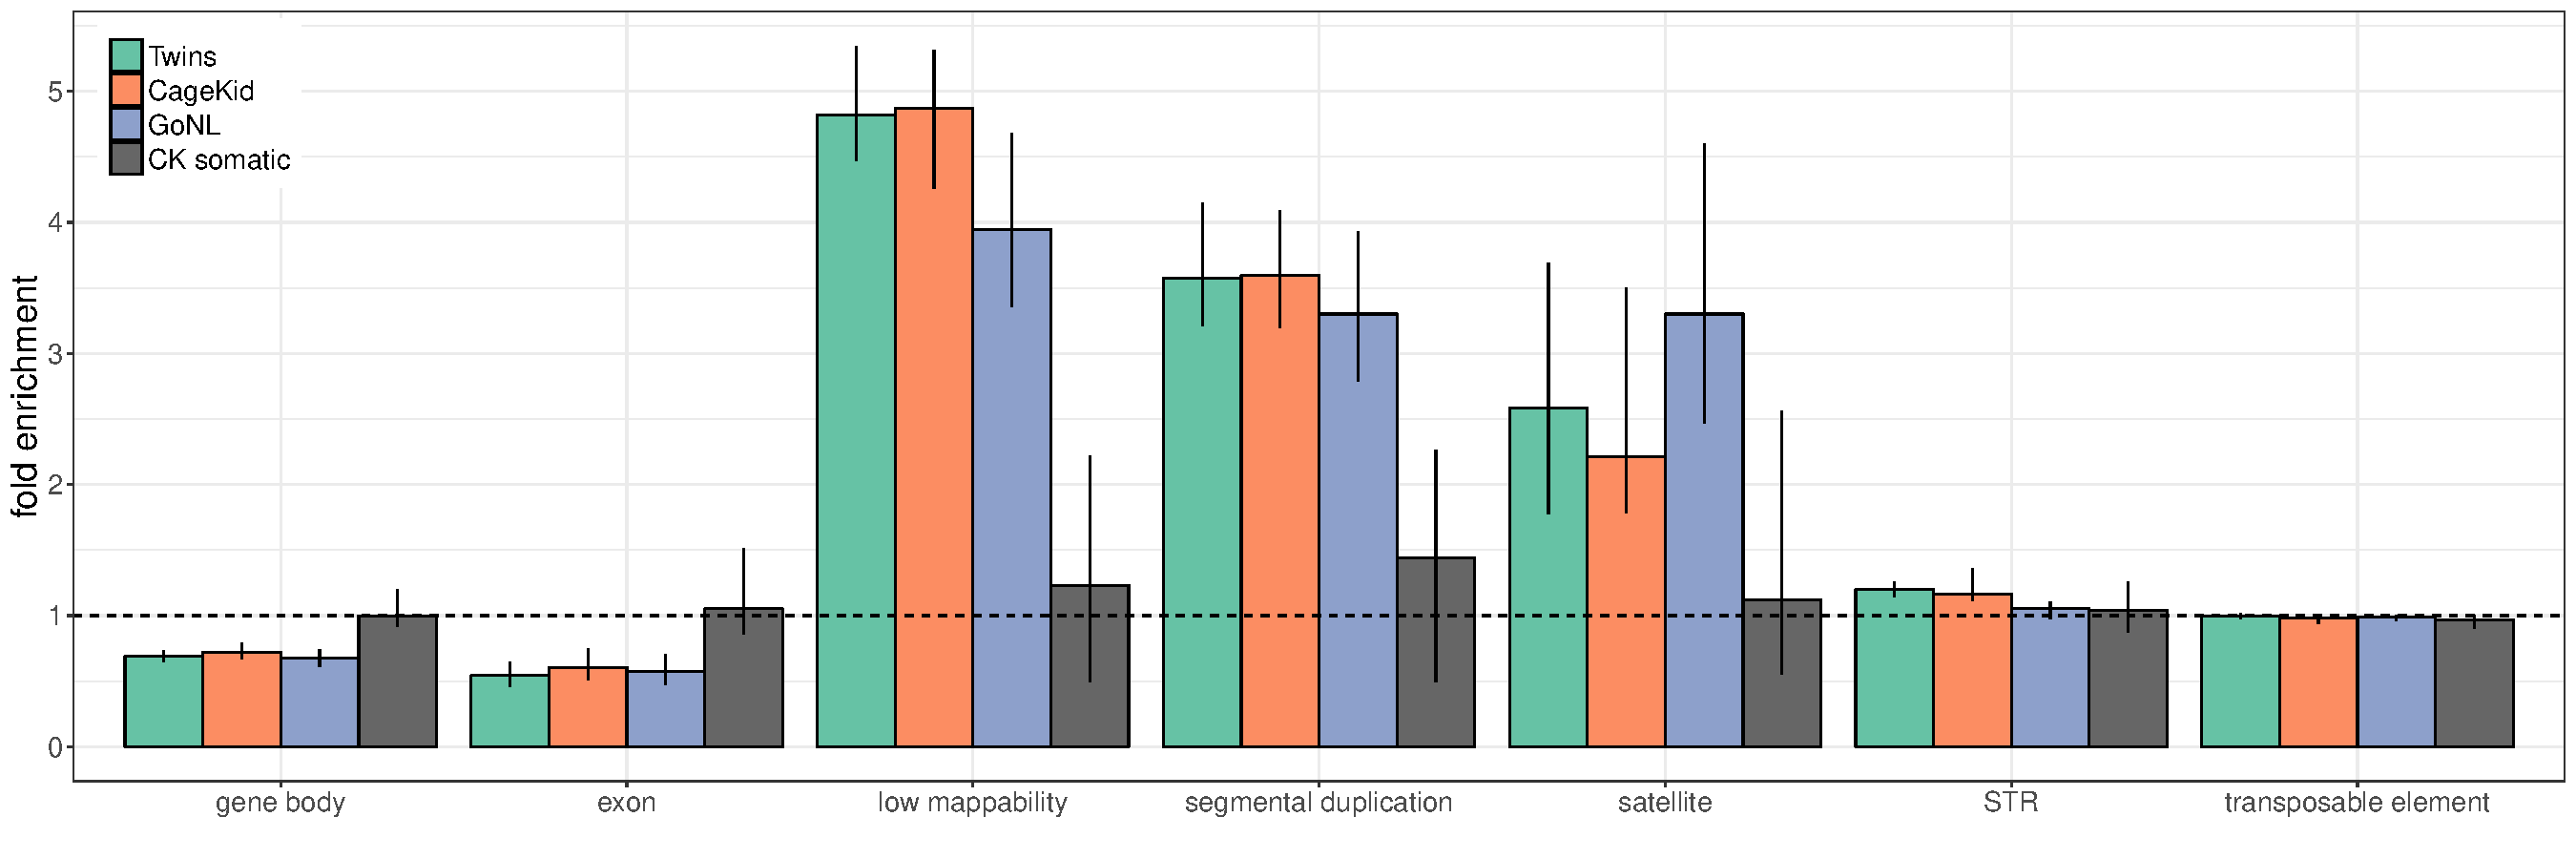
\includegraphics[width=\textwidth, page=1]{figures/PopSV-repeatEnr-long.pdf}
  \caption{}
  \label{fig:repAll}
  \end{subfigure}
  \begin{subfigure}{.9\textwidth}
  \includegraphics[width=\textwidth, page=3]{figures/PopSV-repeatEnr-long.pdf}
  \caption{}
  \label{fig:repFam}
  \end{subfigure}
  \caption[CNVs in normal genomes.]{{\bf CNVs in normal genomes.} {\small a) Enrichment of CNVs in different genomic classes (x-axis) across different cohorts (colors) and controlling for the distance to centromere/telomere/gap. Bars show the median fold enrichment compared to control regions. The error bar represents 90\% of the samples in the cohort. b) Enrichment of CNVs in repeat families (x-axis) controlling for the overlap with segmental duplication and distance to centromere/telomere/gap. The error bars were winsorized at 7 for clarity. {\it STR: Short Tandem Repeat}; {\it TE: Transposable Element}.
    }}
\end{figure}
Segmental duplications (SD), DNA satellites and Short Tandem Repeats (STRs) were also significantly enriched with fold-enrichment of 3.6, 2.6 and 1.2, respectively.
The over-representation of CNVs in SDs has been described before\cite{Sharp2006} and in a recent study \cite{Sudmant2015}, half of the CNV base pairs were shown to overlap a SD.
To investigate the contribution of low-mappability regions beyond SDs, we used matched control regions and included segmental duplication overlap in the logistic regression model.
Even after controlling for this known enrichment, we found that CNVs overlapped low-coverage regions more than twice as much as expected (Fig. \ref{fig:repCont}).
This two-fold enrichment is independent of the SD association and consistently observed in the 3 cohorts of normal genomes.
In contrast to germline CNVs, sCNVs were once again found to be more uniformly distributed (Fig. \ref{fig:repAll} and \ref{fig:repCont}).
These results suggest that the enrichments of germline CNVs near CTGs and in regions of low-mappability are unlikely to be the result of a methodological artifact.

\subsection*{Various repeat families are more prone to harbor CNVs}

We wanted to further characterize the distribution of germline CNVs in relation to different repeat classes and families.
By comparing CNVs to the same control regions with matched overlap with SD and distance to CTGs we can look for patterns that are specific to repeat sub-families without the risk of being biased by the global enrichments (Fig. \ref{fig:repFam}).
Using this approach, we found that CNVs were still significantly enriched in satellites repeats and in short tandem repeats (P-value $<10^{-4}$, Fig. \ref{fig:repCont}), with fold-enrichments of 2.3 and 1.2 respectively.

Although it is known that DNA satellites and simple repeats are more unstable\cite{Eckert2009}, the extent to which CNVs are found in these regions in humans had, to our knowledge, not been systematically explored.
Satellite repeats are grouped into distinct families depending on their repeated unit and we found that not all satellite repeats were equally likely to overlap a CNV (Fig. \ref{fig:repSat}).
In particular, Alpha satellites have the highest and most significant enrichment (P-value $<10^{-5}$), with more than 3 times more CNVs than in the control regions (Fig. \ref{fig:repFam}).
We noted that satellites tend to span completely CNVs (Fig. \ref{fig:repeatOl}), suggesting that satellites are likely directly involved in the CNV formation.
Short and long tandem repeats can be highly polymorphic\cite{Gymrek2012,Warburton2008}.
Constrained by read length, recent studies\cite{Willems2014,Fungtammasan2015} focused on variation of STRs smaller than 100 bp.
In our analysis we found that CNVs were significantly enriched in the largest annotated STRs ($>$100 bp or $>$400 bp, Fig. \ref{fig:repFam}).
STR can be grouped by motif and we further tested the largest and most frequent families (Fig. \ref{fig:repSR}).
Except for the weak enrichment in $AT$ ($TA$) repeats, the STR enrichment appeared mostly independent of the repeat motif.
Here the repeats tend to overlap just a fraction of the variant, but a clear subset of the variants are fully covered by these tandem repeats (Fig. \ref{fig:repeatOl}).
Finally, although transposable elements (TEs) as a whole did not show enrichment (Fig. \ref{fig:repAll}), the ``Other'' repeat class, which contains SVA repeats, was found to be significantly enriched in the two higher depth datasets (Fig. \ref{fig:repFam}). Moreover, looking at TEs at the level of individual repeat families, we found a number of them to be significantly enriched including SVA F or L1Hs.
Notably, HERV-H, an older ERV sub-family, was also in the list of enriched TEs.
This sub-family has been shown to be expressed and important in human embryonic stem cells\cite{Kelley2012,Lu2014}.
Alu elements contributed to the formation of human segmental duplications\cite{Bailey2003} and are often found around SV breakpoints\cite{Kidd2010} but this TE family was not enriched in CNVs in our data.
On the other hand, several families of L1 repeats older than the still active L1HS family were also enriched (e.g. L1PA2 to L1PA4) and often implicated in what appears to be non-allelic homologous recombination (see examples in Fig. \ref{fig:l1pa}).
Reassuringly, the somatic CNVs once again did not show any of these enrichments (Fig. \ref{fig:repFam}).

\subsection*{Impact of CNVs in regions of low-mappability}

Compared to the latest 1000GP catalog\cite{Sudmant2015a}, we identified 3,455 novel regions with CNVs in more than 1\% of the population.
81.3\% of these regions were located in low-mappability regions while 18.4\% were located in extremely low-mappability regions.
These novel CNV regions were missing from the 1000GP catalog and also mostly absent in other recent CNV surveys; only 7.9-15.1\% of the novel regions overlapped with a CNV in three recent CNV catalogs\cite{Handsaker2015,Chiang2017,Francioli2014} (Fig. \ref{fig:novelcatfreq}).
Among the regions with a CNV in the CEPH12878 sample, we identified a deletion in the second intron of the {\it TRIM16} gene that was found by both Pendleton et al.\cite{Pendleton2015} and {\sf PopSV}.
Across the 640 individuals analyzed by {\sf PopSV}, 12\% carried the variant.
Thanks to the long-read data, the exact breakpoints had been pinpointed in Pendleton et al.\cite{Pendleton2015} and it was in fact a SVA-F transposable element located within the 6 Kbp intron in the reference genome but absent from the assembled sequence.
SVA-F is one of the youngest repeat family in the human genome and their high similarity remains a challenge for CNV analysis.
Furthermore, the variant is located within a segmental duplication with 98.5\% similarity and absent from public catalogs such as the 1000GP or GoNL.
Another deletion supported by both public assemblies and local reassembly of the PacBio read was located 12 Kbp downstream of {\it TMPRSS11E}.
6.6\% of the individuals carried the variant in the {\sf PopSV} catalog.
The assembled sequence helped pinpoint the breakpoints to an annotated L1PA2 in the reference genome.
The variant was also located in a segmental duplication and absent from public catalogs such as the 1000GP or GoNL.
Finally, a deletion affecting 8 different exons from the {\it CR1} gene was found by both Pendleton et al.\cite{Pendleton2015} and {\sf PopSV} in CEPH12878.
{\it CR1} has been associated with Alzheimer disease\cite{Lambert2009} and is located within embedded segmental duplications with high similarity.
The deletion was present in 3\% of the population analyzed with {\sf PopSV} but is absent from public CNV catalogs.

Overall, 7,206 protein-coding genes were found to have an exon overlapping a variant in at least one of the 640 normal genomes studied (Table \ref{tab:gene}).
If we included the promoter regions (10 Kbp upstream of the transcription start site), at least 11,341 protein-coding genes were potentially affected by at least one CNV in the population.
Focusing on regions of low-mappability, we found 4,285 different CNVs that were completely included in regions annotated as STR.
These STR-CNVs overlapped the coding sequence of 45 protein-coding genes, and 286 genes when including the promoter region (Table \ref{tab:gene}).
In contrast, for CNVs included in satellite regions, only 21 genes had an exon or the promoter region overlapping one of the 1,822 Satellite-CNVs.
Finally, we focused on CNVs that were novel compared to the 1000GP\cite{Sudmant2015a} and in low-mappability regions.
Even there, 347 genes were found to have an exon overlapping such CNVs and this number increased to 560 when including the promoter regions.
Out of these 347 genes, 29 were previously associated to a mendelian disorder or phenotype in the OMIM database (Online Mendelian Inheritance in Man; \url{http://omim.org/}, Table \ref{tab:omimgenes}).

\begin{table}[htp]
  \centering
  \resizebox{.9\textwidth}{!}{
    \begin{tabular}{|l|r|r|r|r|r|r|r|}
      \hline
      \multirow{2}{*}{Set}                 & \multirow{2}{*}{CNVs} & \multicolumn{3}{c|}{Genes with CNVs} & \multicolumn{3}{c|}{OMIM genes with CNVs}             \\
                                           &                       & Exon                                 & + Promoter & + Intron & Exon  & + Promoter & + Intron \\
      \hline
      \multicolumn{1}{c}{{\it All CNVs}}   & \multicolumn{7}{c}{}                                                                                                 \\
      \hline
      All                                  & 91,735                & 7,206                                & 11,341     & 13,259   & 1,241 & 1,857      & 2,196    \\
      Low coverage                         & 32,707                & 848                                  & 1,491      & 2,648    & 95    & 160        & 371      \\
      Extremely low coverage               & 9,348                 & 304                                  & 401        & 442      & 11    & 14         & 25       \\
      TE                                   & 20,491                & 164                                  & 1,747      & 3,998    & 29    & 233        & 664      \\
      STR                                  & 4,285                 & 45                                   & 286        & 748      & 5     & 39         & 129      \\
      Satellite                            & 1,822                 & 2                                    & 21         & 33       & 0     & 0          & 0        \\
      \hline
      \multicolumn{1}{c}{{\it Novel CNVs}} & \multicolumn{7}{c}{}                                                                                                 \\
      \hline
      All                                  & 17,046                & 418                                  & 680        & 1,102    & 38    & 59         & 135      \\
      Low coverage                         & 15,263                & 347                                  & 560        & 894      & 29    & 47         & 111      \\
      Extremely low coverage               & 6,591                 & 189                                  & 263        & 285      & 5     & 6          & 8        \\
      TE                                   & 3,896                 & 17                                   & 192        & 504      & 1     & 12         & 66       \\
      STR                                  & 1,806                 & 14                                   & 81         & 230      & 0     & 9          & 41       \\
      Satellite                            & 890                   & 1                                    & 4          & 5        & 0     & 0          & 0        \\
      \hline
    \end{tabular}
  }
  \caption[Impact of CNVs on protein-coding genes.]{{\bf Impact of CNVs on protein-coding genes.} {\small The {\it CNVs} number represents the number of different CNVs, after collapsing CNVs with more than 50\% reciprocal overlap. Repeat CNV: more than 90\% of the CNV is annotated as repeat. Genes are protein-coding genes and the promoter region is defined as the 10 Kbp region upstream of the transcription start site. {\it Novel CNVs} are located within regions annotated as novel compared to the 1000 Genome Project catalog.}}
  \label{tab:gene}
\end{table}

\section{Discussion}

Despite the strong interest in CNVs because of their role in diseases, detecting them accurately has remained a challenge, especially in regions of low-mappability. This is mostly due to technical variation in RD that cannot be fully modeled by mappability estimates.
Using a recently developed CNV-calling approach that relies on a set of reference samples to estimate the expected RD\cite{Monlong2018}, we show that it is possible to accurately detect CNVs across the genome, even in repeat-rich regions.
Indeed, using monozygotic twins and normal/tumor pairs, we were able to demonstrate that the performance of {\sf PopSV} was stable and in most cases superior to other methods across different types of low-mappability regions.
Although experimental validation can be challenging in these regions, we were able to confirm a number of deletions using PCR validation as well as variants in some of the most difficult regions by taking advantage of public datasets from long-read sequencing studies.

% New results in repeats
Notably, using {\sf PopSV} on 140 normal genomes with high sequencing depth ($\sim$40X) and 500 additional samples with medium coverage ($\sim$13X), we found that regions of low mappability, which only represent $\sim$10\% of the genome, were around 5 times more likely to harbor CNVs. The fact that this enrichment was observed for germline events and not somatic events was both reassuring and interesting because of the implications on the selection forces at play. In particular, we were able for the first time to quantify the extent to which some regions in the genome are more prone to harbor such structural rearrangements.
For instance, beyond the known enrichment in segmental duplications, we found genome-wide enrichments for different families of DNA satellites, simple repeats and TE, such as SVA, L1Hs and HERV-H.
Moreover, although {\sf PopSV} doesn't fully characterize STR variation, it was able to detect CNVs in large annotated STRs.
These CNVs could complement the output of STR detection methods that look for STR variation within sequencing reads and for this reason cannot test STRs longer than $\sim$100 bp.
Here, we found a strong CNV enrichment in STRs larger than 400 bp suggesting that large STRs should be included in genome-wide STR variation screens.
Overall, having a more complete CNV catalog enabled an unbiased characterization of the CNV patterns across the genome and could potentially increase the power for trait-association studies.

Fine-tuning the location of breakpoints is often possible by reanalyzing the local read coverage or using orthogonal methods such as split-read or local assembly.
In repeat-rich regions however, these methods generally do not perform well.
Long read sequencing is currently the only experimental method that actually results in unambiguous SV calls with nearly quasi-base-pair resolution in low-mappability regions.
Indeed, recent studies using long-read sequencing\cite{Chaisson2014,Pendleton2015} found many novel SVs and highlighted variation involving complex repetitive DNA.
The increased resolution and ability to span repeated regions expanded existing SV catalogs but only a handful of genomes have been sequenced in this way so far due to the higher cost of this technology.
Although breakpoint and allele characterization is limited with short reads, we were able to detect the presence of such CNVs across a large population of normal genomes.
Compared to previous studies, our CNV catalog strongly overlaps with the variants found by long-read sequencing studies in low-mappability regions.
With hundreds of genomes at our disposal we identified frequent CNVs in repeat-rich regions that had escaped previous population-scale surveys.
In the CEPH12878 sample, we independently identified low-mappability variants and showed that some novel deletions were recurrent in our cohort.
For example, an exonic deletion in the {\it CR1} gene absent from public CNV catalogs was identified by the long-read sequencing and found in $\sim$3\% of the samples tested by {\sf PopSV}.
{\it CR1} has been associated with Alzheimer Disease\cite{Lambert2009} thus this exonic deletion in a low-mappability region might be relevant for association studies.
Using our full CNV catalog, we identified 3,455 novel regions that were not present in 1000G public SV database\cite{Sudmant2015a} but found in more than 1\% of our 640 genomes.
These regions overlapped exons of 418 protein-coding genes, 38 of which were associated with a disease phenotype in the OMIM database.
The amount of genes hit by CNVs in novel or low-mappability regions and the enrichment of CNVs in repeat-rich regions suggest that they be included in genome-wide surveys.
As other types of variant are likely enriched in repeat-rich regions, we anticipate that population-based methods, such as {\sf PopSV}, will facilitate the identification not only of CNVs but also of other types of SVs in both normal and cancer genomes.

% Extensions and breakpoint resolution
One of the most promising future development of PopSV to further characterize low-mappability regions is its extension to detect balanced SV such as inversions or translocations.
Indeed, instead of modeling the coverage of properly mapped reads, the same population-based strategy could test for an excess of discordant reads.
By counting the number of reads in incorrect orientation or joining distant regions, one could recognize an excess of SV-supporting reads from discordant mapping caused by repeats.
Such an approach could detect inversions and translocations that contains repeats around their breakpoints or complement SV calls from orthogonal approaches by providing a robust confidence score based on abnormal read coverage.


\section{Data and Code Availability}

The {\sf PopSV} R package and documentation are available at \url{http://jmonlong.github.io/PopSV/}.
The scripts and instructions to reproduce the graphs and numbers in this study have been deposited at \url{http://github.com/jmonlong/reppopsv/} and archived in \url{https://doi.org/10.5281/zenodo.1241137}.

\section{Accessions numbers}

The CNV catalog and annotations were deposited at \url{https://figshare.com/s/8fd3007ebb0fbad09b6d}.
The raw sequences of the different datasets had already been deposited by their respective consortium (see \nameref{sec:suppmat:reppopsv}).


\section{Acknowledgments}

We are grateful to the team of the Qu\'ebec Study of Newborn twins who provided the twin dataset and the Cagekid consortium who provided the renal cancer dataset.
This study also made use of data generated by the Genome of the Netherlands Project.
A full list of the investigators is available from \url{www.nlgenome.nl}.
Funding for the project was provided by the Netherlands Organization for Scientific Research under award number 184021007, dated July 9, 2009 and made available as a Rainbow Project of the Biobanking and Biomolecular Research Infrastructure Netherlands (BBMRI-NL).
The sequencing was carried out in collaboration with the Beijing Institute for Genomics (BGI).
Finally, we would like to thank Simon Gravel, Mathieu Blanchette, Mathieu Bourgey and Toby Dylan Hocking for helpful discussions.

\section{Funding}

This work was supported by a grant from the National Sciences and Engineering Research Council (NSERC-448167-2013) and a grant from the Canadian Institute for Health Research (CIHR-MOP-115090).
SLG and GB are supported by the Fonds de Recherche Sant\'e Qu\'ebec (FRSQ-29493 and FRSQ-25348).
Data analyses were enabled by compute and storage resources provided by Compute Canada and Calcul Qu\'ebec.


%%% Local Variables:
%%% mode: latex
%%% TeX-master: "../main"
%%% End:


\chapter{Discussion of Results and Implications}
\label{chap:disc}


\section*{Population-based approaches and whole-genome sequencing}
% Population-based approach improves sensitivity and resolution. Useful for many applications, cancer, disease, repeats.
The three chapters highlighted the usefulness of population-based approach to detect genomic variation.
The superior sensitivity made it possible to detect somatic variants in tumor samples, small and non-coding variants in epilepsy patients and variants in low-mappability regions in healthy individuals.
% The results and implications that stemmed from these variants are described below.
The main results and implications concerning ccRCC, epilepsy and repeat-rich regions have been described in their respective chapters.
However, all these results relied on a first step of variant detection that used the same strategy: analyzing a genome in the context of many to minimize the effect of technical noise. 
This population-based approach can benefit variant calling as long as the genomes in the population are sequenced with similar protocol and machine, and the raw data is pre-processed with the same pipeline.
If this is the case, other factors that don't affect technical variation, for example gender or ethnicity, should not affect the variant calling.
The main result of this work, at least in term of methodology, is the demonstrated power of population-based approach across multiple applications.

All three chapters used WGS data across dozens or hundreds of genomes.
At the beginning of this work, WGS data across that many samples was not widespread.
Large-scale sequencing projects used to be rare and international efforts involving numerous centers\cite{Lander2001,Durbin2010}.
Yet, the cost of sequencing has been steadily decreasing and new machines currently advertise sub-1000\$ costs for whole-genome sequencing.
As a result, sequencing projects involving hundreds of genomes are more and more common.
Motivated by the future opportunities for personalized medicine, hundreds of genomes are being sequenced to characterize the population in different countries\cite{Francioli2014,Wong2013,Gudbjartsson2015}.
For disease studies as well, whole genome sequencing of hundreds of participants has been performed or is currently under way.
Large-scale project that focus on single disease include the MSSNG collaboration\footnote{\url{https://www.mss.ng}} that aims at sequencing 10,000 families affected by autism and whose first results were published recently\cite{Yuen2017} and the Alzheimer's Disease Sequencing Project\cite{Beecham2017} which is sequencing more than a thousand patients with Alzheimer disease.
WGS is also at the core of multi-disease projects that are currently in progress.
The Genomics England initiative\footnote{\url{https://www.genomicsengland.co.uk}} will sequence 100,000 genomes from patients with rare diseases and cancers while the TOPMed consortium\footnote{\url{https://www.nhlbiwgs.org/}} plans on sequencing the genome of 120,000 individuals to study the contribution of genetics to heart, lung, blood and sleep disorders.
Often, this data is first processed at the individual level and later pooled to derive population information or association metrics.
Our data highlights the benefit of pooling individuals earlier in the analysis workflow.
Instead of pooling results after variant calling, we found that variant calling could be significantly improved thanks to population information.
I believe that population-based approaches similar to {\sf PopSV} could have a large impact on the variant discovery across these large-scale projects.
It is regrettable to have information across hundreds of other experiments and to keep it aside for variant calling. 
Of note, promising avenues are currently being explored to reverse this trend, for example by integrating population information even before variant calling.
The new field of genome graphs aims at constructing a reference genome that includes known variation in order to directly improve read mapping, variant calling and population representation.

%% WGS
In addition to the population-based approach, our results also contribute to the case for whole-genome sequencing when designing a large scale genomic study.
Although more costly than genotyping arrays or exome sequencing, WGS can detect a larger range of variants: rare and frequent, coding and non-coding, SNVs and CNVs or other SVs.
WGS data produced with a primary objective in mind can often be re-used to study different aspects of genomic variation.
For example, the data used in Chapter \ref{chap:loy} was originally produced to describe somatic SNVs and broad CNV patterns in ccRCC\cite{Scelo2014}.
In Chapter \ref{chap:loy}, we re-analyzed this dataset to further investigate the arm-level aberrations across the cohort and more precisely estimate the amount of somatic LOY in tumors from male patients.
These results were replicated with a PCR-based approach in a different cohort of tumors and represent the foundation of the functional importance of somatic LOY advocated in our study.
In chapter \ref{chap:epi} and \ref{chap:rep}, the combination of WGS and {\sf PopSV} was also instrumental in discovering novel scientific results.
Novel coding variants in epilepsy or low-mappability regions were identified.
A CNV profile that had never been associated with epilepsy, rare non-coding CNVs, was for the first time seen to be strongly enriched close to known epilepsy genes.
Thousands of low-mappability regions that frequently experience CNV were identified, including some located near or within protein-coding genes.

\section*{Somatic loss of Y and gender imbalance in cancer}

The gender imbalance in the renal cancer incidence is not completely understood.
Our results suggest that somatic LOY occurs frequently in male tumors and have a functional impact.
Hence, loss of chromosome Y could explain part of the higher incidence in males.
Other cancers, such as liver and bladder cancers, show gender imbalance toward males and might also be partly explained by LOY\cite{Siegel2017}.
Several studies have found that more than 30\% of tumors from these cancers experienced LOY\cite{Sauter1995,Park2006}.
Our study and others suggest that LOY could be a driver mechanism of tumor progression by disregulating tumor suppressors, such as {\it KDM5D} and {\it KDM6C}.
Of note, {\it KDM5D} and {\it KDM6C} are both expressed in the liver and the bladder.
Because of the multiple similarities with our study of ccRCC, it is sensible to speculate that the same mechanism, that is downregulation of {\it KDM5D} and {\it KDM6C} through LOY, is involved in the tumor progression of cancers of the liver and bladder.
A population-based approach such as the one we used might identify more subtle LOY in sequencing datasets which could help estimate the rate and impact of this type of variation.

Although incidental, we detected LOY in the blood samples as well, both in the WGS and the PCR-based replication.
As described in the literature, somatic LOY in blood was associated with older age in our cohort.
Two studies suggest that the presence of LOY in blood samples can be associated with higher incidence rate of non-hematological cancers or Alzheimer disease\cite{Forsberg2014,Dumanski2016}.
Unfortunately, due to the absence of matched healthy controls we couldn't directly test the association with ccRCC.
We found no significant associations between LOY in blood and the tumor stage or grade.
Further investigations in the future will require more samples, including matched controls and balanced numbers of different tumor grades.


\section*{Small and non-coding CNVs in epilepsy and neurological disorders}

Our results suggest that WGS will be necessary to fully characterize the genetic factors associated with epilepsy.
First, WGS is more suitable for CNV detection compared to other sequencing approaches (e.g. exome sequencing).
Despite its successes in detecting rare SNVs associated with genetic disorders, exome sequencing is less suited for CNV and SV detection.
Indeed, the step that captures the regions of interest adds another layer of technical bias.
Not only is the read coverage affected by the capture efficiency in each region, the fragmented representation of the genome also hinders the sensitive detection of CNVs.
Considering the importance of CNVs in epilepsy as shown by our study and others, WGS will be key to efficiently detect even exonic variants associated with the disease.
Second, we show for the first time an association between non-coding CNVs and epilepsy.
Thanks to WGS, we were able to interrogate the presence of both small and non-coding variants.
In contrast, previous array-based study were limited to large CNVs which tended to overlap exonic regions.
We found a clear enrichment of rare non-coding CNVs in patients close to genes that were previously associated with epilepsy.
Even more convincing, the enrichment increased the closer to the exon and was boosted for deletions and variants overlapping regulatory regions.
Similar results were found in individuals with autism where non-coding {\it de novo} CNVs and SNVs were enriched up to 100 Kbp from autism-associated genes\cite{Turner2016}.

These conclusions are relevant for epilepsy but also for other neurological disorders.
Large CNVs have also been associated with autism\cite{Pinto2010}, mental retardation\cite{Mefford2009} and schizophrenia\cite{Walsh2008,Marshall2016}.
\begin{comment}
  Genes in neurological pathways tend to be large and organized in large gene families often located within segmental duplications. 
\end{comment}
In each disease, the same pattern emerged: probands tend to have rare large CNVs and/or in hotspot regions flanked by segmental duplications.
Often, the same CNV hotspot regions have been associated with several neurological disorders as is the case for 1q21.1, 15q13.3 and 16p11.2\cite{Mefford2009}.
Based on these commonalities and our results, I expect that small and non-coding CNVs play a role in other neurological disorders as well.
In general, the study of the genetics of neurological disorder could greatly benefit from WGS approaches similar to the one we used in chapter \ref{chap:epi}.

The enhanced resolution of WGS and our population-based approach suggest that some types of variants had been missed before.
The inclusion of such genomic variants might help characterize the exact syndrome or grouping patients with similar etiology.
Drug resistance is an important problem in idiopathic epilepsy and much remains to be done to understand its causes.
The study presented in chapter \ref{chap:epi} contributes to the identification of genes that might be associated with epilepsy and advocates for the inclusion of small and non-coding CNVs in the genomic profile of epilepsy patients.
It is my hope that either these candidate genes or the inclusion of those variants will one day help to devise new drugs or to assist clinician when choosing a treatment.


\section*{Including low-mappability regions in genome-wide studies}

More and more evidence supports the importance of repeated regions in disease and human phenotypes.
After being considered junk DNA for a long period, the role of many types of repeats is becoming clear.
From the highly variable STRs and their association with gene expression changes\cite{Gymrek2016}, to the contribution of TEs in regulation networks\cite{Bourque2009} or the satellite instability in cancer\cite{Kim2013}, repeats are gathering more attention.
Still, repeats are under-studied because of the technical challenges and reluctant mentality shift.
Our results show that WGS and a population-based approach is sufficient to detect CNV in many repeat-rich regions.
Moreover, we found that these regions are more likely to harbor CNVs compared to the rest of the genome.
Many low-mappability regions are also located close to protein-coding genes, some of which have been linked to Mendelian diseases before.
By masking repeats, genome-wide association studies have discarded a small part of the genome but a large fraction of the genomic variation.
I believe that approaches similar to the one presented in this work, as well as future technologies that will make repeat integration easier, could lead to a better genomic characterization of diseases and human phenotypes.




\chapter{Conclusions and Future Directions}
\label{chap:conc}

The population-based approaches presented here have been successful at detecting somatic and challenging germline changes in copy number but more remains to be done.
Although we were able to detect the presence of variation, more effort will be necessary to fully characterize the alternate alleles.
The methods could also be extended to other sequencing technologies, particularly targeted sequencing such as whole-exome sequencing.
Similar approaches could also be extended to other types of SVs, for example translocations and inversions.
Finally, recent technological advances shine a promising light on the future of SV characterization.
Genome editing might help investigate the functional impact of non-coding CNVs while new sequencing technologies will likely be used in concert to integrate SVs and low-mappability in genomics studies.

\section*{From variant detection to base-pair resolution}
% Long reads are the shit, but expensive shit.
The population-based approach presented in this work is powerful to detect variation but cannot fully characterize the variants.
Deriving the exact sequence of the mutated allele or breakpoints remains challenging in repeat-rich regions or for complex SVs.
Indeed, large sample sizes and population-oriented analysis are mostly able to flag the presence of an abnormal signal in these regions.
To unlock a base-pair level resolution for the breakpoints or the variant sequence in general, a different type of data will be necessary rather than more of the same data.
In WGS early years, genomes were sequenced at low depth and pooling individuals helped increase read support necessary to estimate the variant sequences.
A typical WGS genome is now often 30x deep or more and pooling reads across different individuals will have only marginal benefit on the base-pair resolution of the SVs.
At this depth, the problematic variants are either in repeat-rich regions or more complex than the canonical SV types.
More of the same short reads wouldn't bring much new information and the ambiguity would likely remain.
In the end, the short read size is the main limitation.
Hence, long read sequencing will likely have a large impact on characterizing many of the SVs that remain challenging.
Several studies already showed the power of long reads for SV detection\cite{Chaisson2014,Pendleton2015}.
Unfortunately the higher cost of these technologies limits their use.
The cost and usage might change but it is unlikely that a very large number of genome will be sequenced with these technologies.
Still, this technology could be used to validate and confirm SVs identified in large scale short-read projects.
By carefully choosing a few genomes to sequence, the catalog of complex and repeat-rich SVs could be greatly improved.
For example, sequencing genomes carrying candidate pathogenic variants could validate and provide more insights into the variant impact or potential mechanism of action.
Selecting a few genomes with different complex SVs and low-mappability variants could also maximize the gain from each long-read sequencing experiment.
In summary, long-read sequencing of a few carefully selected genomes would nicely complement deep short-read sequencing across large cohorts.
Of note, a more cost effective approach would be to capture the regions containing the SVs detected from the large-scale short-read surveys.
The challenge here is to efficiently and accurately capture large and potentially repeat-rich regions.
If this type of capture is possible, Sanger sequencing could also be used to characterize the variants at the base-pair level.
Having a validated set of variants at the base-pair level and covering low-mappability regions will also provide an extremely useful gold-standard to assess the sensitivity and specificity of CNV methods.
In the absence of such a gold-standard, we had to rely on indirect assessment, such as the replication in twins or the comparison with just a few long-read assemblies.

\section*{Extension to targeted sequencing}
% Other application WES/targeted sequencing
Targeted sequencing involve a step of capture in which the desired genomic regions are selectively amplified.
Thanks to the capture, only a set of regions, for example coding regions, are sequenced.
However, the capture efficiency varies depending on the design and regions, introducing additional technical variation in the read coverage.
CNV detection from the read coverage is challenging as a result.
Existing methods turned to population-based approach, similar to our WGS method {\sf PopSV}, in order to normalize read coverage using other experiments that used similar capture\cite{Shi2013,Talevich2014}.
{\sf PopSV} could be easily extended to such application as it doesn't rely on coverage uniformity but rather considers each region separately in the context of reference samples.
We actually ran {\sf PopSV} successfully on several whole-exome sequencing projects with minimal changes.
Briefly, one additional step in the pipeline was necessary: the removal of regions that were not covered by the sequencing experiment.
Of note, the quality control step was even more important here in order to ensure that the reference and tested samples originated from the same sequencing protocol.
Indeed, capture protocols are continuously evolving with new exome capture kits available every year.
Although we believe that the normalization used by {\sf PopSV} is superior to several of existing methods, the regions with abnormal coverage are merged using a simplistic approach.
For WGS, it is natural to merge consecutive regions that share a CNV signal as they are located one next to the other.
In targeted sequencing, there are often stretches of non-covered regions that separate captured regions.
By integrating this information a better segmentation can be performed as shown by several methods\cite{Fromer2012,Magi2013}.
In the context of an extension to targeted sequencing, we could improve {\sf PopSV}'s segmentation step with such algorithms in order to have both a more advanced normalization and an appropriate segmentation.

\section*{Extension to balanced structural variation}
% Other application: other types of SVs (balanced)
{\sf PopSV} could also be extended to other types of SVs, as the name originally intended.
Currently, abnormal coverage of properly mapped reads identifies regions with a change in copy number.
In the future, {\sf PopSV} could operate on the coverage of reads with discordant paired-end mapping.
For example, reads whose pair couldn't be aligned or aligned at an abnormal distance or orientation.
An abnormal excess of discordant reads would be a sign of SV.
With {\sf PopSV}'s population-based approach, discordant mapping due to repeats will be corrected for and only regions with a real excess of discordant mapping should be called.
This type of test could be run across genomic regions, as for the CNV analysis, or between pairs genomic regions.
The objective of the paired-regions approach is to increase the signal-to-noise ratio between the SV-caused discordant reads and the background level.
Indeed, the background level of discordant reads in a region might be high enough to drown the signal from the additional reads created by the SV.
When focusing on discordant read pairs with one read mapped to a region and the other in another distant region, the amount of background discordant mapping is much lower.
The excess of discordant read pair linking the boundaries of a translocation or an inversion might be more easily detected.
Both of these approaches are currently being tested.
The original scan, i.e. testing one region at a time, seems to be under-powered and return much fewer calls than the CNV scan.
Alternatively, this extension of {\sf PopSV} would also be useful to annotate calls from other methods, for example those that identify clusters of discordant or split reads.
These methods tend to suffer from a high false-positive rate most likely due to repeat confusion.

\section*{Investigating the functional impact of non-coding CNVs}

We identified dozens of rare non-coding CNVs located close to known epilepsy genes and absent from our controls and public CNV databases.
The most promising candidates are located in regions that were previously associated with changes in the gene expression and are predicted to host regulatory regions.
While the frequency and location of these non-coding CNVs are encouraging, it is not clear which variant really has an impact on the gene and eventually the disease phenotype.
Indeed, we observed a clear enrichment which means that some CNVs are associated with the disease.
In order to narrow down the list of candidate regions we could either increase the sample size or experimentally test the variant's impact.
Both strategies have their own set of challenges.

To achieve a higher sample size, more patients are necessary and might require national or international collaboration.
Because epilepsy is a diverse disease, the new patients should be matched as much as possible with our cohort in order to maximize the chances of observing recurrent variants.
Finally, the number of probands that need to be sequenced to identify single genes or non-coding regions might be unrealistically high, again because of the diverse phenotype and complex gene network involved in the disease mechanism.

Investigating deeper our current candidates might be more feasible thanks to recent advances in cell reprogramming and DNA editing.
It is not feasible to study live human brains and unpractical to collect post-mortem brains in correct conditions for functional assays.
Cell reprogramming provides a better alternative.
By reprogramming cells from a carrier into relevant cell types, e.g. neurons, the effect of a variant on the gene function could be tested in the laboratory.
If patients' samples are unavailable or to better control for the genetic background, DNA editing like CRISPR-Cas9 could recreate the non-coding deletion in cells.
DNA editing before cell differentiation would provide a culture of cells that could then be differentiated into different cell types to extensively study the effect of the variants.
While a true ``epilepsy'' phenotype is almost impossible to test in a cell culture, we could investigate the effect of the variants on gene expression or other molecular phenotypes.
Although this approach requires time, resources and expertise, it is more geared toward validating our non-coding candidates and more likely to give conclusive results.

\section*{SV and WGS in the near future}

Thanks to better sequencing technologies and methods, systematic {\it de novo} assembly of genomes might eventually supplant the re-sequencing approach that is dominant today.
The optimal output would be phased sequence for each genome that is sequenced and assembled.
SV detection would then come down to comparing the assembled genomes.
Recent advances in long-read, linked-read, or conformation capture sequencing greatly improve the quality of the {\it de novo} assemblies and contains long-range information useful for phasing.
However, for SV detection, long-read sequencing will be necessary to reach a base-pair resolution across the full genome, as mentioned above.
Because of its cost, only a limited number of genomes will be sequenced with long-read sequencing in the near future.
Furthermore, hundreds of thousands of genomes have been sequenced or are being sequenced with short-read technology.
Until affordable and comprehensive {\it de novo} assembly is available, the field will likely move to hybrid strategies for SV analysis.
But how could we integrate SV information from different approaches and across hundreds to thousands of genomes?
The recent development of genome graphs provides a promising solution\cite{Paten2017}.
Genome graphs represent the genome and genomic variation in a population using a graph structure.
One of its current form corresponds to the current reference genome augmented with SNVs and indels from the 1000 Genomes Project\cite{Garrison2017}.
Genome graphs are by nature flexible so that we could imagine further improving their breadth with high-quality {\it de novo} assemblies or SV catalogs from long-read sequencing datasets.
Using a genome graph populated with the high-resolution variants, SV could be more efficiently genotyped in short-reads datasets across large populations.
Genome graphs also provide an ideal structure to represent complex haplotypes, such as those involving SVs.
As for other types of variants, haplotype information will be invaluable to assist variant calling and to predict the functional impact of SVs.
Short-read datasets could benefit from the long-range information present in the high-resolution datasets by integrating complex haplotype information in the genome graphs.
With coordination and data sharing, and with genome graphs as a new reference system, there is hope that we can rapidly reach the point where phased high-resolution SVs can be genotyped accurately from short-read datasets spanning hundreds of thousands of genomes.




%%% Local Variables:
%%% mode: latex
%%% TeX-master: "../main"
%%% End:


\newpage
\singlespacing
\bibliographystyle{unsrtnat5}
\bibliography{thesis-fixed}


\chapter*{Appendices\markboth{APPENDICES}{}}
\addcontentsline{toc}{chapter}{Appendices}

\section*{Appendix A}
\addcontentsline{toc}{section}{Appendix A: Significant Contributions to Other Projects}
\label{append:other}
% {\it Maybe better in the Contributions section ?}

The contribution of the thesis author to other published works during the thesis period is listed below.
\bigskip

\noindent Contribution in another project from the Canadian Epilepsy Network (CENet):

\begin{itemize}  
\item F.~F. Hamdan, C.~T. Myers, P.~Cossette, P.~Lemay, D.~Spiegelman, A.~D. Laporte,
  C.~Nassif, O.~Diallo, {\bf J.~Monlong}, M.~Cadieux-Dion, S.~Dobrzeniecka,
  C.~Meloche, K.~Retterer, M.~T. Cho, J.~A. Rosenfeld, W.~Bi, C.~Massicotte,
  M.~Miguet, L.~Brunga, B.~M. Regan, K.~Mo, C.~Tam, A.~Schneider,
  G.~Hollingsworth, D.~R. FitzPatrick, A.~Donaldson, N.~Canham, E.~Blair,
  B.~Kerr, A.~E. Fry, R.~H. Thomas, J.~Shelagh, J.~A. Hurst, H.~Brittain,
  M.~Blyth, R.~R. Lebel, E.~H. Gerkes, L.~Davis-Keppen, Q.~Stein, W.~K. Chung,
  S.~J. Dorison, P.~J. Benke, E.~Fassi, N.~Corsten-Janssen, E.-J. Kamsteeg,
  F.~T. Mau-Them, A.-L. Bruel, A.~Verloes, K.~{\~{O}}unap, M.~H. Wojcik, D.~V.
  Albert, S.~Venkateswaran, T.~Ware, D.~Jones, Y.-C. Liu, S.~S. Mohammad,
  P.~Bizargity, C.~A. Bacino, V.~Leuzzi, S.~Martinelli, B.~Dallapiccola,
  M.~Tartaglia, L.~Blumkin, K.~J. Wierenga, G.~Purcarin, J.~J. O'Byrne,
  S.~Stockler, A.~Lehman, B.~Keren, M.-C. Nougues, C.~Mignot, S.~Auvin,
  C.~Nava, S.~M. Hiatt, M.~Bebin, Y.~Shao, F.~Scaglia, S.~R. Lalani, R.~E.
  Frye, I.~T. Jarjour, S.~Jacques, R.-M. Boucher, E.~Riou, M.~Srour,
  L.~Carmant, A.~Lortie, P.~Major, P.~Diadori, F.~Dubeau, G.~D'Anjou,
  G.~Bourque, S.~F. Berkovic, L.~G. Sadleir, P.~M. Campeau, Z.~Kibar, R.~G.
  Lafreni{\`{e}}re, S.~L. Girard, S.~Mercimek-Mahmutoglu, C.~Boelman, G.~A.
  Rouleau, I.~E. Scheffer, H.~C. Mefford, D.~M. Andrade, E.~Rossignol, B.~A.
  Minassian, and J.~L. Michaud.
\newblock {High Rate of Recurrent De Novo Mutations in Developmental and
  Epileptic Encephalopathies}.
\newblock \emph{The American Journal of Human Genetics}, 101\penalty0
  (5):\penalty0 664--685, nov 2017.
\newblock \doi{10.1016/j.ajhg.2017.09.008}.
\end{itemize}

\noindent Contributions to projects not directly relevant for the thesis topic:

\begin{itemize}
\item M.~Mele, P.~G. Ferreira, F.~Reverter, D.~S. DeLuca, {\bf J.~Monlong}, M.~Sammeth,
  T.~R. Young, J.~M. Goldmann, D.~D. Pervouchine, T.~J. Sullivan, R.~Johnson,
  A.~V. Segre, S.~Djebali, A.~Niarchou, GTEx~Consortium, F.~A. Wright,
  T.~Lappalainen, M.~Calvo, G.~Getz, E.~T. Dermitzakis, K.~G. Ardlie, and
  R.~Guigo.
\newblock {The human transcriptome across tissues and individuals}.
\newblock \emph{Science}, 348\penalty0 (6235):\penalty0 660--665, may 2015.
\newblock \doi{10.1126/science.aaa0355}.

\item D.~D. Pervouchine, S.~Djebali, A.~Breschi, C.~A. Davis, P.~P. Barja, A.~Dobin,
  A.~Tanzer, J.~Lagarde, C.~Zaleski, L.-H. See, M.~Fastuca, J.~Drenkow,
  H.~Wang, G.~Bussotti, B.~Pei, S.~Balasubramanian, {\bf J.~Monlong}, A.~Harmanci,
  M.~Gerstein, M.~A. Beer, C.~Notredame, R.~Guig{\'{o}}, and T.~R. Gingeras.
\newblock {Enhanced transcriptome maps from multiple mouse tissues reveal
  evolutionary constraint in gene expression.}
\newblock \emph{Nature communications}, 6:\penalty0 5903, jan
  2015{\natexlab{a}}.
\newblock \doi{10.1038/ncomms6903}.

\item {\bf J.~Monlong}, M.~Calvo, P.~G. Ferreira, and R.~Guig{\'{o}}.
\newblock {Identification of genetic variants associated with alternative
  splicing using sQTLseekeR}.
\newblock \emph{Nature Communications}, 5\penalty0 (May):\penalty0 4698, aug
  2014.
\newblock \doi{10.1038/ncomms5698}.

\item P.~G. Ferreira, P.~Jares, D.~Rico, G.~Gomez-Lopez, A.~Martinez-Trillos,
  N.~Villamor, S.~Ecker, A.~Gonzalez-Perez, D.~G. Knowles, {\bf J.~Monlong},
  R.~Johnson, V.~Quesada, S.~Djebali, P.~Papasaikas, M.~Lopez-Guerra,
  D.~Colomer, C.~Royo, M.~Cazorla, M.~Pinyol, G.~Clot, M.~Aymerich, M.~Rozman,
  M.~Kulis, D.~Tamborero, A.~Gouin, J.~Blanc, M.~Gut, I.~Gut, X.~S. Puente,
  D.~G. Pisano, J.~I. Martin-Subero, N.~Lopez-Bigas, A.~Lopez-Guillermo,
  A.~Valencia, C.~Lopez-Otin, E.~Campo, and R.~Guigo.
\newblock {Transcriptome characterization by RNA sequencing identifies a major
  molecular and clinical subdivision in chronic lymphocytic leukemia}.
\newblock \emph{Genome Research}, 24\penalty0 (2):\penalty0 212--226, feb 2014.
\newblock \doi{10.1101/gr.152132.112}.

\item T.~Lappalainen, M.~Sammeth*, M.~R. Friedl{\"{a}}nder*, P.~a.~C. {‘t Hoen}*,
  {\bf J.~Monlong}*, M.~a. Rivas*, M.~Gonz{\`{a}}lez-Porta, N.~Kurbatova, T.~Griebel,
  P.~G. Ferreira, M.~Barann, T.~Wieland, L.~Greger, M.~van Iterson,
  J.~Alml{\"{o}}f, P.~Ribeca, I.~Pulyakhina, D.~Esser, T.~Giger, A.~Tikhonov,
  M.~Sultan, G.~Bertier, D.~G. MacArthur, M.~Lek, E.~Lizano, H.~P.~J. Buermans,
  I.~Padioleau, T.~Schwarzmayr, O.~Karlberg, H.~Ongen, H.~Kilpinen, S.~Beltran,
  M.~Gut, K.~Kahlem, V.~Amstislavskiy, O.~Stegle, M.~Pirinen, S.~B. Montgomery,
  P.~Donnelly, M.~I. McCarthy, P.~Flicek, T.~M. Strom, H.~Lehrach,
  S.~Schreiber, R.~Sudbrak, {\'{A}}.~Carracedo, S.~E. Antonarakis,
  R.~H{\"{a}}sler, A.-C. Syv{\"{a}}nen, G.-J. van Ommen, A.~Brazma,
  T.~Meitinger, P.~Rosenstiel, R.~Guig{\'{o}}, I.~G. Gut, X.~Estivill, and
  E.~T. Dermitzakis.
\newblock {Transcriptome and genome sequencing uncovers functional variation in
  humans}.
\newblock \emph{Nature}, sep 2013.
\newblock \doi{10.1038/nature12531}.
\end{itemize}



%%% Local Variables:
%%% mode: latex
%%% TeX-master: "../main"
%%% End:


\clearpage
 
\section*{Appendix B}
\addcontentsline{toc}{section}{Appendix B: Supplementary Materials from Chapter \ref{chap:loy}}
\label{append:loy}
Supplementary material for chapter \ref{chap:loy} and its corresponding manuscript: {\bf Loss of chromosome Y leads to down regulation of {\it KDM5D} and {\it KDM6C} epigenetic modifiers in clear cell renal cell carcinoma}.


%% Create counter for supp figs ("S1" etc)
\setcounter{figure}{0}
\renewcommand{\thefigure}{S\ref{chap:loy}.\arabic{figure}}
\setcounter{table}{0}
\renewcommand{\thetable}{S\ref{chap:loy}.\arabic{table}}

\section*{Supplementary Tables}

\begin{table}[ht]
  \centering
  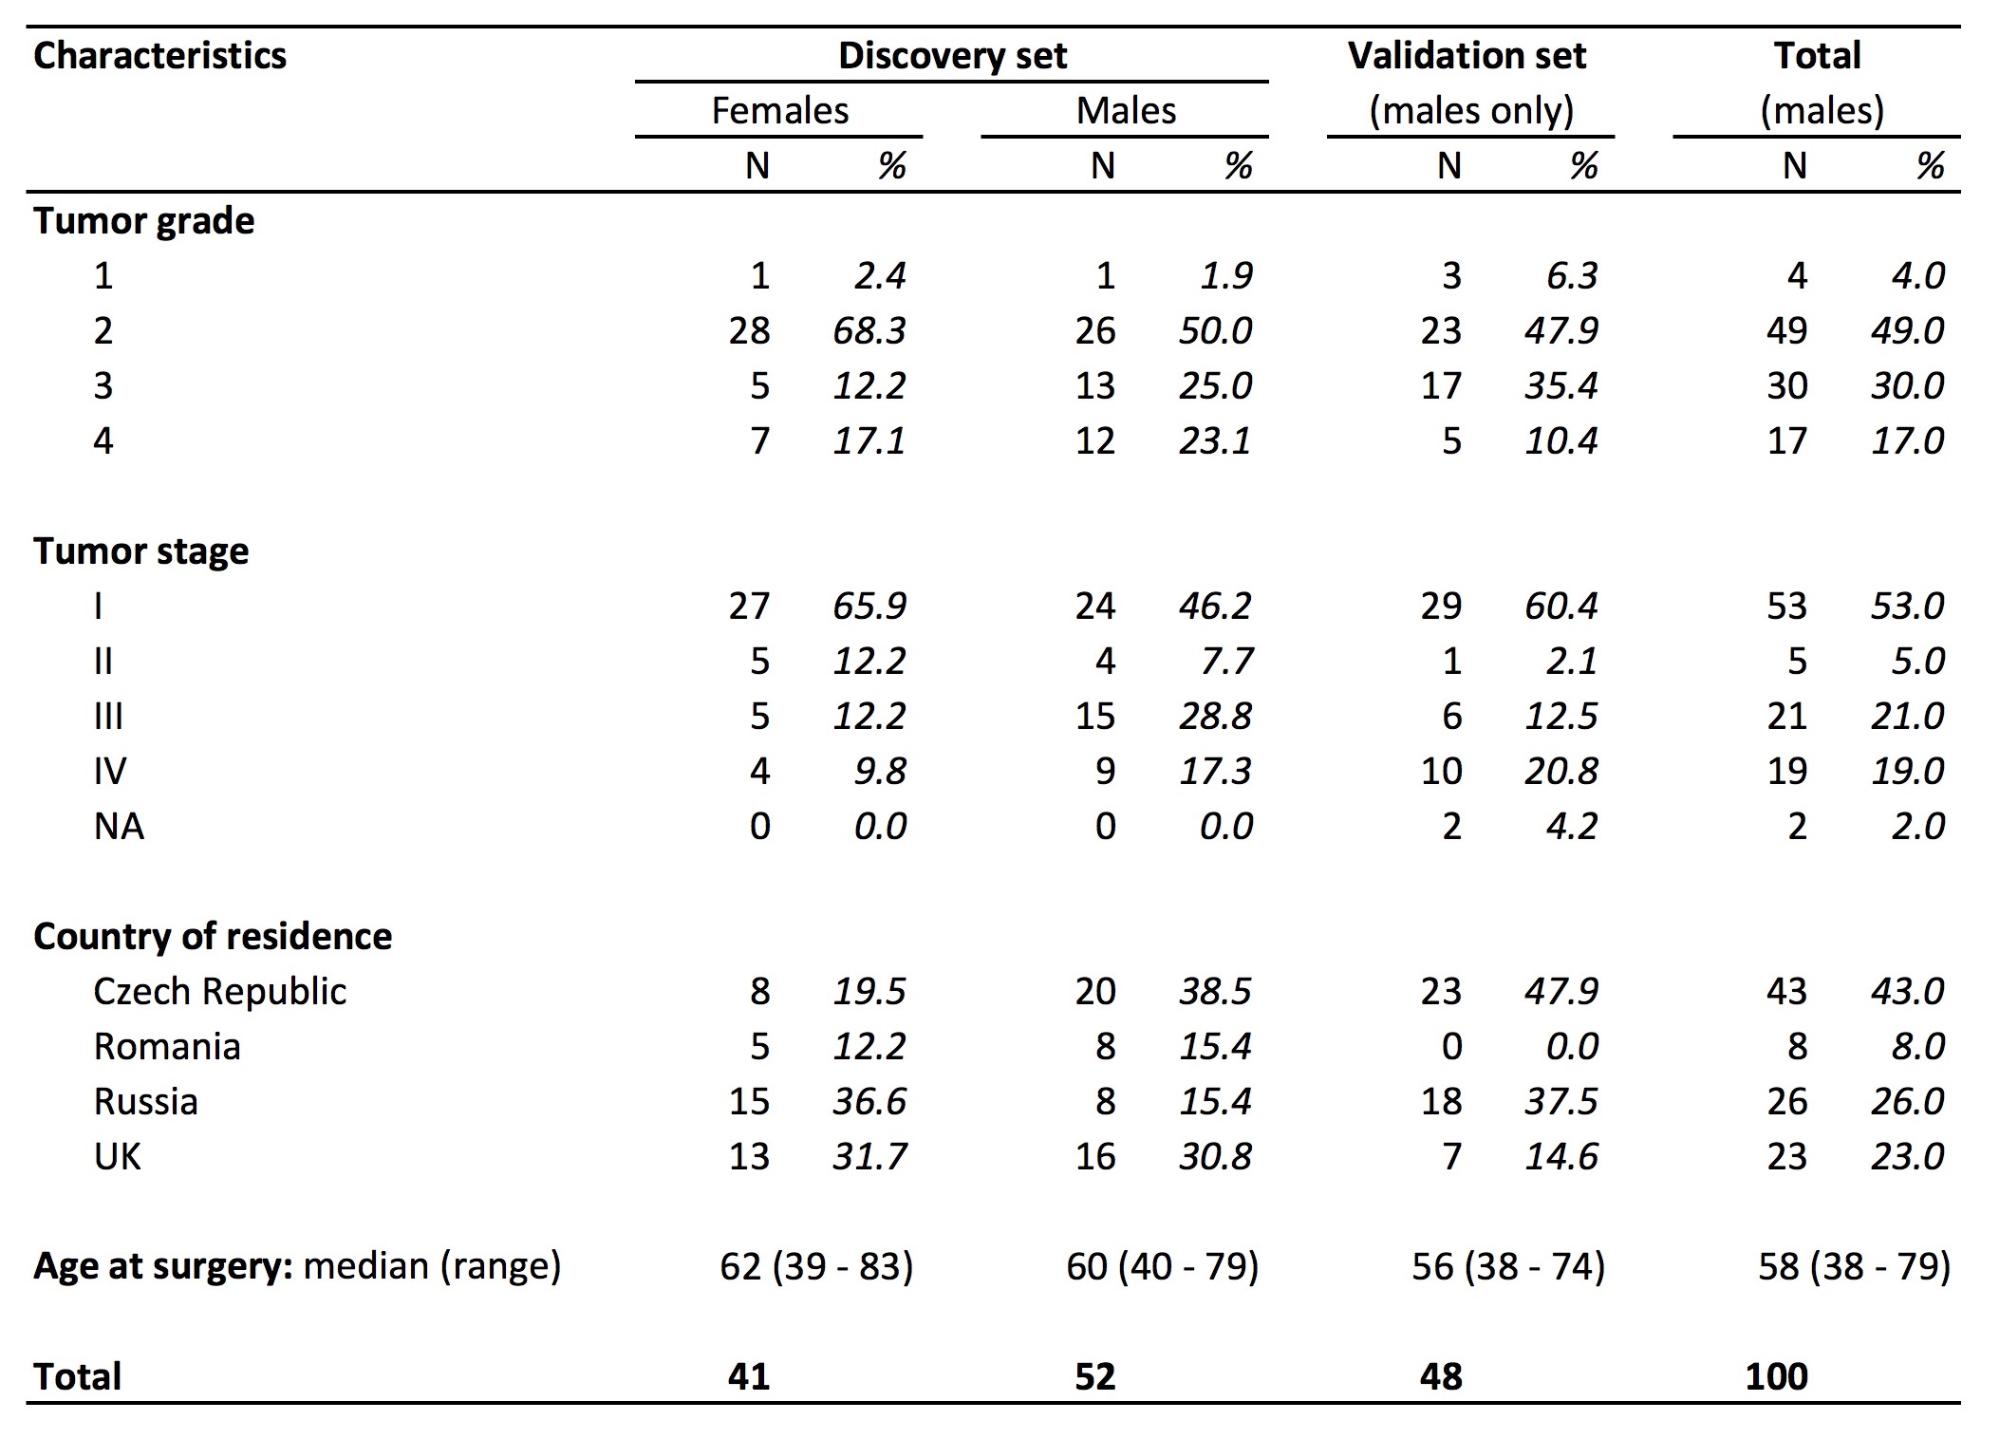
\includegraphics[width=.9\linewidth]{figures/LOY-tabS1.jpg}
  \caption[Characteristics of patients included in the study]{{\bf Characteristics of patients included in the study.}}
  \label{tab:loyS1}
\end{table}

\begin{table}[ht]
  \centering
  \begin{tabular}{lcc}
    Gene           & Chromosome & Fold-change               \\
                   &            & (Differential expression) \\
    \hline
   {\it KDM5D}     & Y          & -1.3                      \\
   {\it USP9Y}     & Y          & -1.4                      \\
   {\it ZFY}       & Y          & -1.1                      \\
   {\it UTY/KDM6C} & Y          & -1.2                      \\
   {\it NLGN4Y}    & Y          & -0.8                      \\
   {\it DDX3Y}     & Y          & -1.8                      \\
   {\it EIF1AY}    & Y          & -1.8                      \\
   {\it TMSB4Y}    & Y          & -0.9                      \\
   {\it RPS4Y1}    & Y          & -2.6                      \\
    \hline
  \end{tabular}
  \caption[Genes differentially expressed between tumors with and without somatic LOY]{{\bf Genes differentially expressed between tumors with and without somatic LOY.} {\small Fold-change of differential expression between the two tumor sets.}}
  \label{tab:loyS2}
\end{table}

\clearpage

\section*{Supplementary Figures}

\begin{figure}[ht]
  \centering
  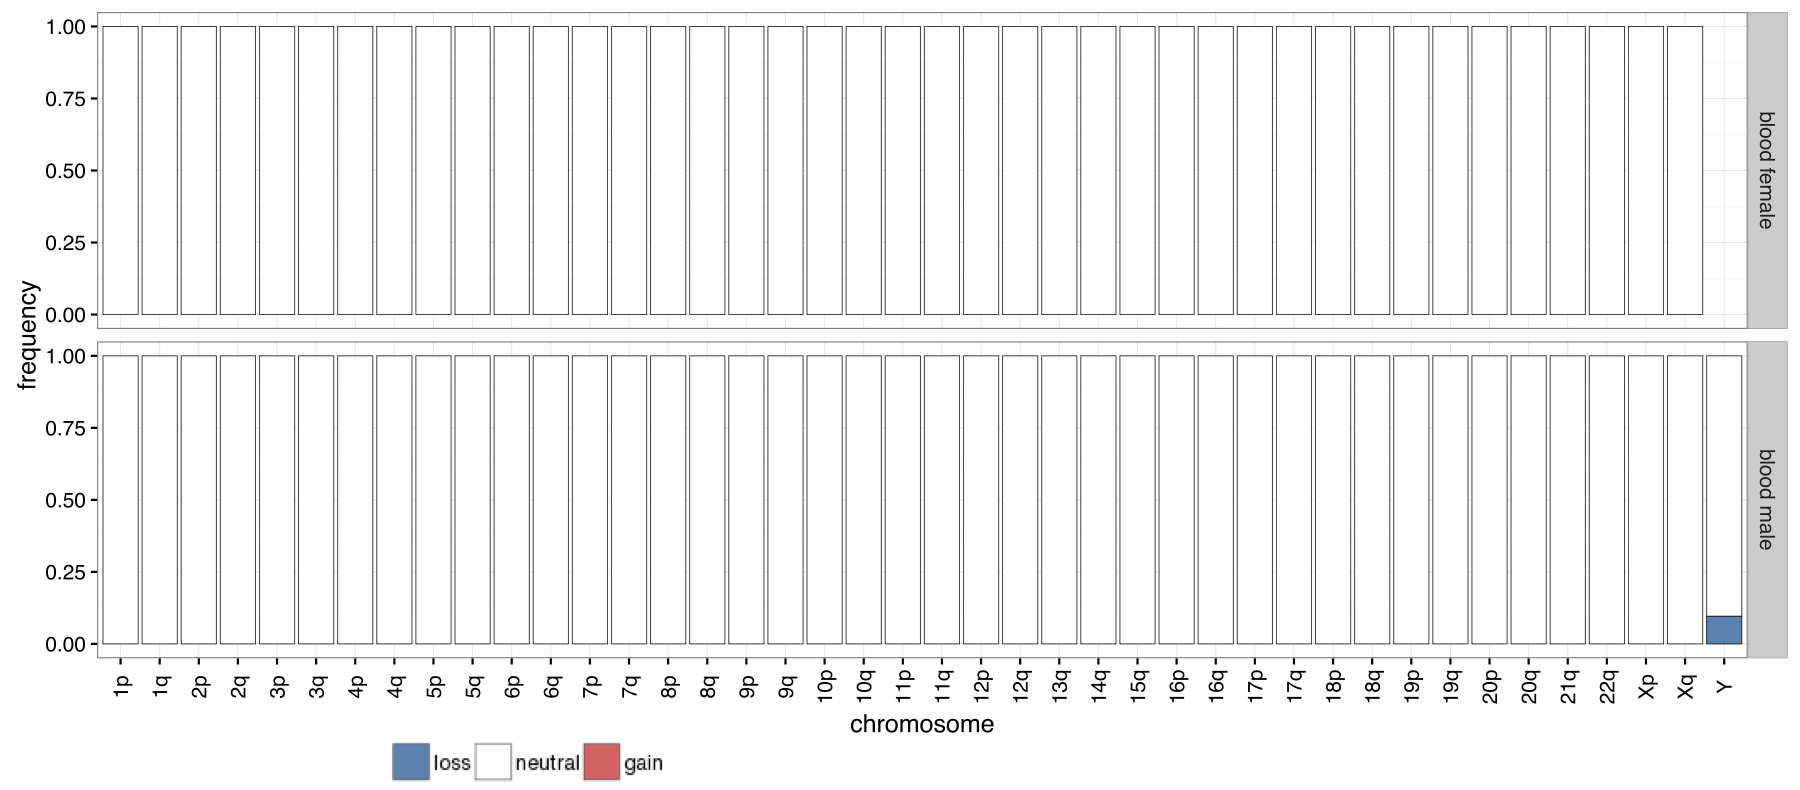
\includegraphics[width=.9\linewidth]{figures/LOY-figS1.png}
  \caption[Copy number analysis in peripheral blood.]{{\bf Copy number analysis in peripheral blood.} {\small Bar graphs show the frequency of copy number variations across the genome in peripheral blood. Frequencies are presented in samples from female and male cases separately.}}
  \label{fig:loyS1}
\end{figure}

\begin{figure}[ht]
  \centering
  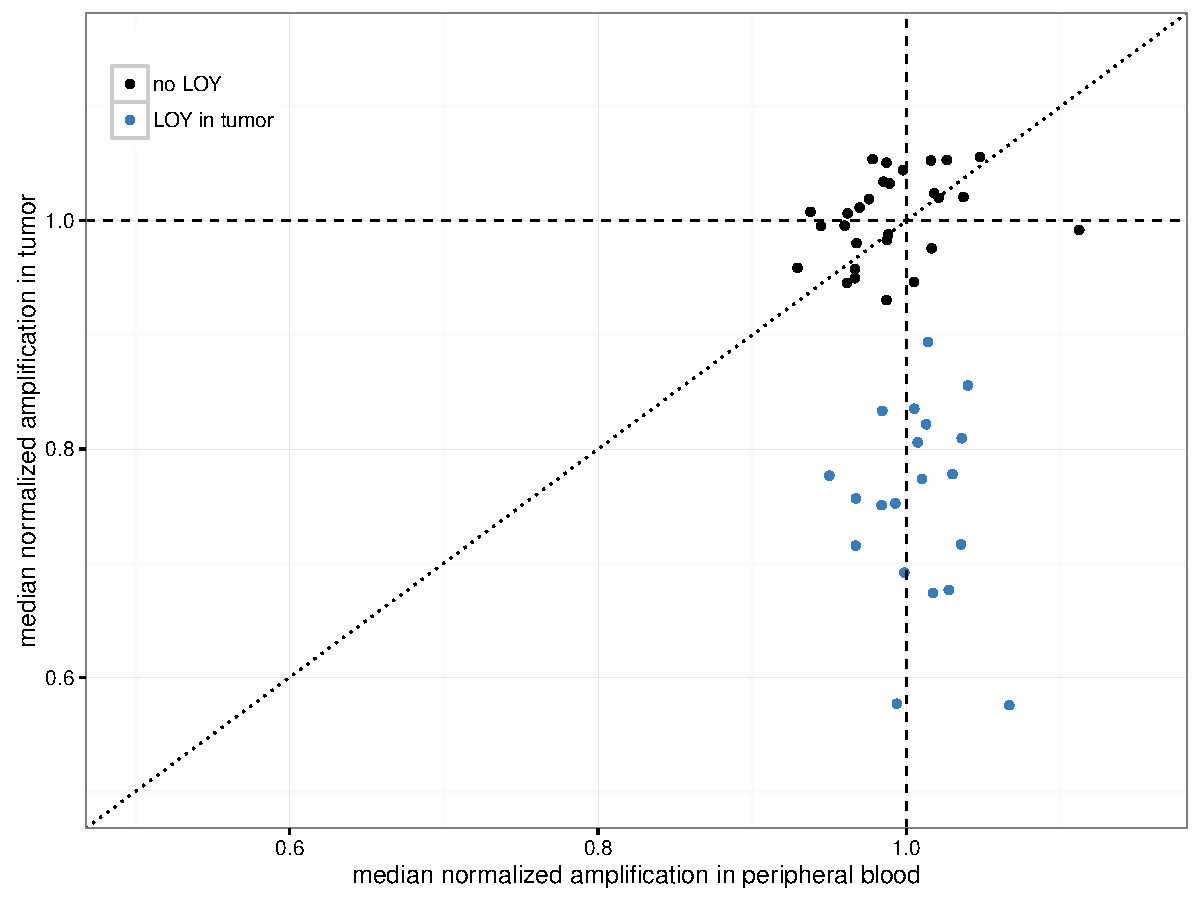
\includegraphics[width=.9\linewidth]{figures/Cagekid-LOY-PCR-fig.pdf}
  \caption[Validation using PCR amplification.]{{\bf Validation using PCR amplification.} {\small Status of chromosome Y in tumors and patient-matched normal samples is shown for individual male subjects of the validation set. The PCR amplification values are normalized and summarized by their median in each sample. Individuals affected by somatic LOY are shown in blue}}
  \label{fig:loyS2}
\end{figure}

\begin{figure}[ht]
  \centering
  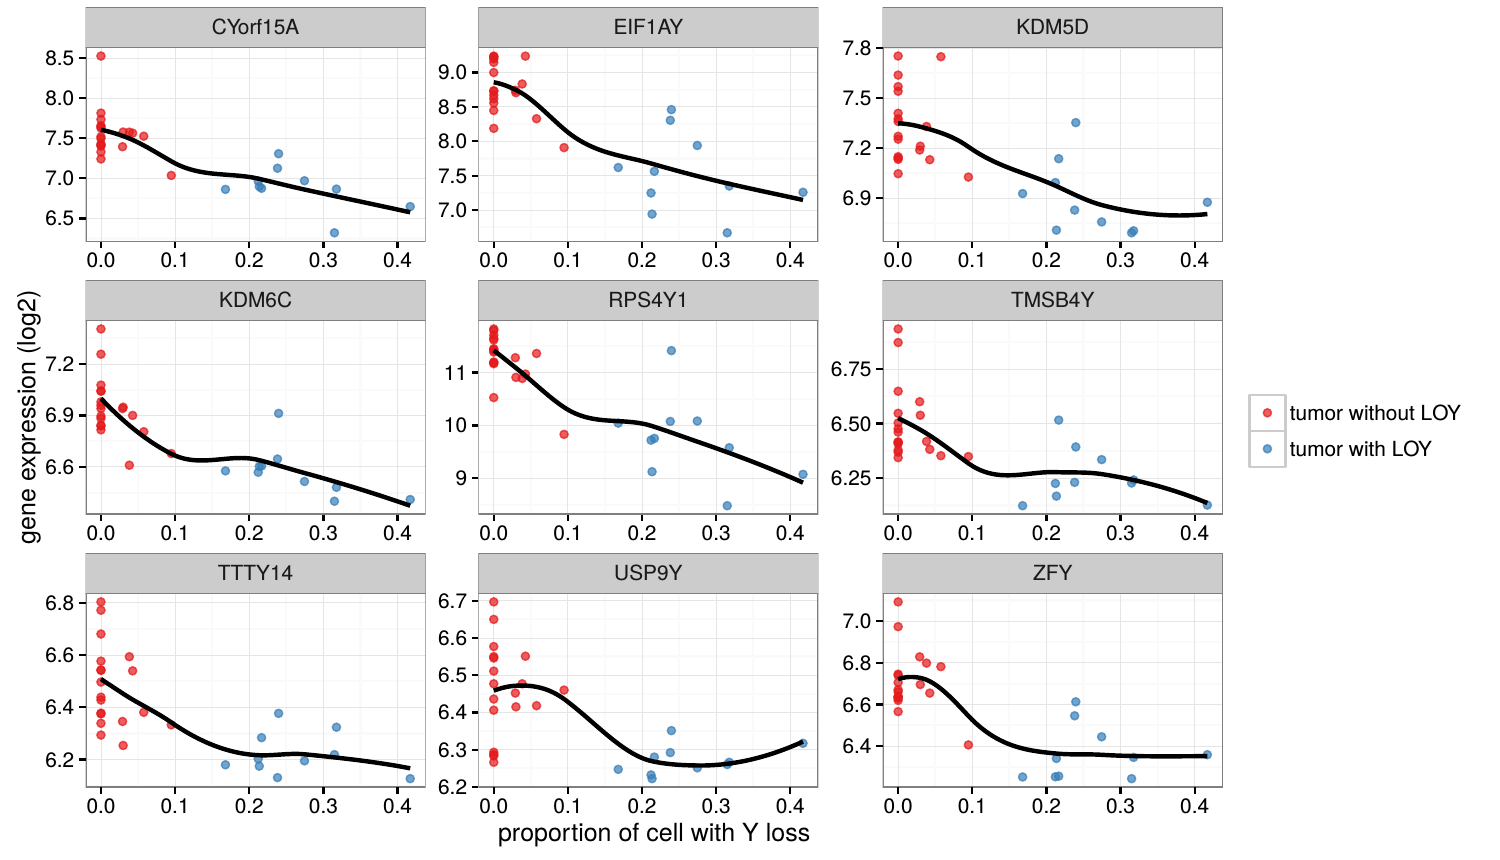
\includegraphics[width=.9\linewidth]{figures/Cagekid-LOY-fig3-array.png}
  \caption[Somatic LOY Y-linked genes down-regulation from array-based expression experiments.]{{\bf Somatic LOY Y-linked genes down-regulation from array-based expression experiments.} {\small The proportion of cells with Y loss was estimated by the PCR amplification values.}}
  \label{fig:loyS3}
\end{figure}

\begin{figure}[ht]
  \centering
  \includegraphics[width=.7\linewidth, page=5]{figures/Cagekid-LOY-fig.pdf}
  \caption[Copy number aberrations of sex chromosomes
and genomic status of X-linked epigenetic modifying genes in tumors of
female and male patients.]{{\bf Copy number aberrations of sex chromosomes
and genomic status of X-linked epigenetic modifying genes in tumors of
female and male patients.} {\small Nearly half of the female tumors harboring
somatic LOX are also affected by mutations of {\it KDM5C}}}
  \label{fig:loyS4}
\end{figure}


\begin{figure}[ht]
  \centering
  \includegraphics[width=.8\linewidth, page=6]{figures/Cagekid-LOY-fig.pdf}
  \caption[Detecting loss of Y.]{{\bf Detecting loss of Y.} {\small The main Gaussian, fitted on the median normalized coverage, is used to detect significant loss/gain. Each male sample, blood and tumor, is colored according to its loss/gain status.}}
  \label{fig:loyS5}
\end{figure}



%%% Local Variables:
%%% mode: latex
%%% TeX-master: "../main"
%%% End:


\clearpage

\section*{Appendix C}
\addcontentsline{toc}{section}{Appendix C: Supplementary Materials from Chapter \ref{chap:epi}}
\label{append:epi}
Supplementary material for chapter \ref{chap:epi} and its corresponding manuscript: {\bf Global characterization of copy number variants in epilepsy patients from whole genome sequencing}.

\section*{Supplementary Tables}

%% Create counter for supp figs ("S1" etc)
\setcounter{figure}{0}
\renewcommand{\thefigure}{S\ref{chap:epi}.\arabic{figure}}
\setcounter{table}{0}
\renewcommand{\thetable}{S\ref{chap:epi}.\arabic{table}}

\begin{table}[htp]
  \caption[{\sf PopSV} calls validated by RT-PCR.]{{\bf {\sf PopSV} calls validated by RT-PCR.} {\small The Excel file contains the location of each region, the CNV type, the number of carriers in the CENet cohorts, the maximum proportion of carriers in the CNV databases, Taqman probe ID and validation status. \url{https://doi.org/10.1371/journal.pgen.1007285.s003}}}
  \label{tab:validation}
\end{table}

\begin{table}[htp]
  \centering
  \resizebox{\textwidth}{!}{.
    \begin{tabular}{|l|l|p{.3\textwidth}|l|l|l|l|l|l|}
      \hline
      {\bf Patient } & {\bf Epilepsy type } & {\bf Syndrome }                                                       & {\bf Copy } & {\bf Chr. } & {\bf CNV start } & {\bf CNV end } & {\bf Exon disrupted }   & {\bf Taqman probe } \\
                     &  &                                                        & {\bf number } &  &  & &    &  \\
      \hline
      CNET0188       & Focal                & Mesial temporal lobe sclerosis                                        & 1                   & 2          & 141335001        & 141365000      & {\it LRP1B}                  & Hs02078420\_cn      \\
      \hline
      CNET0084       & Focal                & Temporal lobe                                                         & 1                   & 4          & 120205001        & 120280000      & {\it USP53};{\it FABP2};{\it C4orf3}     & Hs04813260\_cn      \\
      \hline
      CNET0143       & Generalized          & Childhood absence epilepsy                                            & 1                   & 5          & 65055001         & 65465000       & {\it NLN};{\it ERBB2IP};{\it SREK1}       & Hs03552554\_cn      \\
      \hline
      CNET0151       & Generalized          & Eyelid myoclonia epilepsy with absence                                & 1                   & 9          & 8600001          & 8770000        & {\it PTPRD}                   & Hs06875003\_cn      \\
      \hline
      CNET0041       & Generalized          & Idiopathic generalized epilepsies                                     & 1                   & 11         & 62625001         & 62645000       & {\it SLC3A2}                 & Hs03777991\_cn      \\
      \hline
      CNET0066       & Generalized          & Idiopathic generalized epilepsies                                     & 1                   & 13         & 67325001         & 67575000       & {\it PCDH9}                  & Hs06378870\_cn      \\
      \hline
      CNET0025       & Generalized          & Early onset absence epilepsy (onset <4, absence with or without GTCs) & 1                   & 15         & 60735001         & 60805000       & {\it RORA};{\it NARG2}             & Hs05369880\_cn      \\
      \hline
      CNET0195       & Focal                & Occipital lobe epilepsy                                               & 1                   & 22         & 34095001         & 34200000       & {\it LARGE}                  & Hs05575584\_cn      \\
      \hline
      CNET0005       & Generalized          & febrile sz, child onset GTCs                                          & 1                   & 22         & 41960001         & 42050000       & {\it PMM1};{\it DESI1};{\it CSDC2};{\it XRCC6} & Hs05580065\_cn      \\
      \hline
    \end{tabular}
  }
  \caption{Other pathogenic profiles.}
  \label{tab:supp}
\end{table}

\begin{table}[htp]
  \caption[Clinical features of epileptic patients.]{{\bf Clinical features of epileptic patients.} {\small The Excel file contains the type of epilepsy, age of onset, sex, family history, pharmaco-resistance and potential intellectual disabilities. \url{https://doi.org/10.1371/journal.pgen.1007285.s002}}}
  \label{tab:clinical}
\end{table}

\clearpage

\section*{Supplementary Figures}


%% Figures start here
\begin{figure}[htp]
  \centering
  \begin{subfigure}[b]{.48\textwidth}
    \includegraphics[width=\linewidth,page=5]{figures/epilepsy-biasWGS.pdf}
    \caption{}
    \label{fig:bias:var}
  \end{subfigure}
  \begin{subfigure}[b]{.48\textwidth}
    \includegraphics[width=\linewidth,page=6]{figures/epilepsy-biasWGS.pdf}
    \caption{}
    \label{fig:bias:rank}
  \end{subfigure}
  \caption[Variation and bias in whole-genome sequencing experiments in the epilepsy cohort.]{{\bf Variation and bias in whole-genome sequencing experiments in the epilepsy cohort.} {\small a) Distribution of the bin inter-sample standard deviation coverage (red) and null distribution (blue: bins shuffled, green: simulated normal distribution). b) Proportion of the genome in which a given sample (x-axis) has the highest (red) or lowest (blue) RD. In the absence of bias all samples should be the most extreme at the same frequency (dotted horizontal line). }}
  \label{fig:bias:varrank}
\end{figure}

\begin{figure}[htp]
  \centering
  \begin{subfigure}[b]{.3\textwidth}
    \includegraphics[width=\linewidth,page=4]{figures/cagekid-biasWGS.pdf}
    \caption{}
  \end{subfigure}
  \begin{subfigure}[b]{.3\textwidth}
    \includegraphics[width=\linewidth,page=4]{figures/twin-biasWGS.pdf}
    \caption{}
  \end{subfigure}
  \begin{subfigure}[b]{.3\textwidth}
    \includegraphics[width=\linewidth,page=4]{figures/twin-biasWGS-QDNAseq.pdf}
    \caption{}
  \end{subfigure}

  \begin{subfigure}[b]{.3\textwidth}
    \includegraphics[width=\linewidth,page=5]{figures/cagekid-biasWGS.pdf}
    \caption{}
  \end{subfigure}
  \begin{subfigure}[b]{.3\textwidth}
    \includegraphics[width=\linewidth,page=5]{figures/twin-biasWGS.pdf}
    \caption{}
  \end{subfigure}
  \begin{subfigure}[b]{.3\textwidth}
    \includegraphics[width=\linewidth,page=5]{figures/twin-biasWGS-QDNAseq.pdf}
    \caption{}
  \end{subfigure}

  \begin{subfigure}[b]{.3\textwidth}
    \includegraphics[width=\linewidth,page=6]{figures/cagekid-biasWGS.pdf}
    \caption{}
  \end{subfigure}
  \begin{subfigure}[b]{.3\textwidth}
    \includegraphics[width=\linewidth,page=6]{figures/twin-biasWGS.pdf}
    \caption{}
  \end{subfigure}
  \begin{subfigure}[b]{.3\textwidth}
    \includegraphics[width=\linewidth,page=6]{figures/twin-biasWGS-QDNAseq.pdf}
    \caption{}
  \end{subfigure}
  \caption[Variation and bias in whole-genome sequencing experiments in CageKid and the twin dataset.]{{\bf Variation and bias in whole-genome sequencing experiments in the normals from CageKid (a,d,g), the twin dataset (b,e,h) and the twin dataset after using {\sf QDNAseq}\cite{Scheinin2014} correction (c,f,i).} {\small a-c) Distribution of the bin inter-sample standard deviation coverage (red) and null distribution (blue: bins shuffled, green: simulated normal distribution). d-f) Same for the bin inter-sample standard deviation coverage. g-i) Proportion of the genome in which a given sample (x-axis) has the highest (red) or lowest (blue) RD. In the absence of bias all samples should be the most extreme at the same frequency (dotted horizontal line). }}
  \label{fig:wgsbias2}
\end{figure}

\begin{figure}[htp]
  \begin{subfigure}[b]{.48\textwidth}
    \includegraphics[width=\linewidth,page=2]{figures/cagekid-5kbp-normComparison.pdf}
    \caption{}
    \label{fig:zscoreEx:worstZ}
  \end{subfigure}
  \begin{subfigure}[b]{.48\textwidth}
    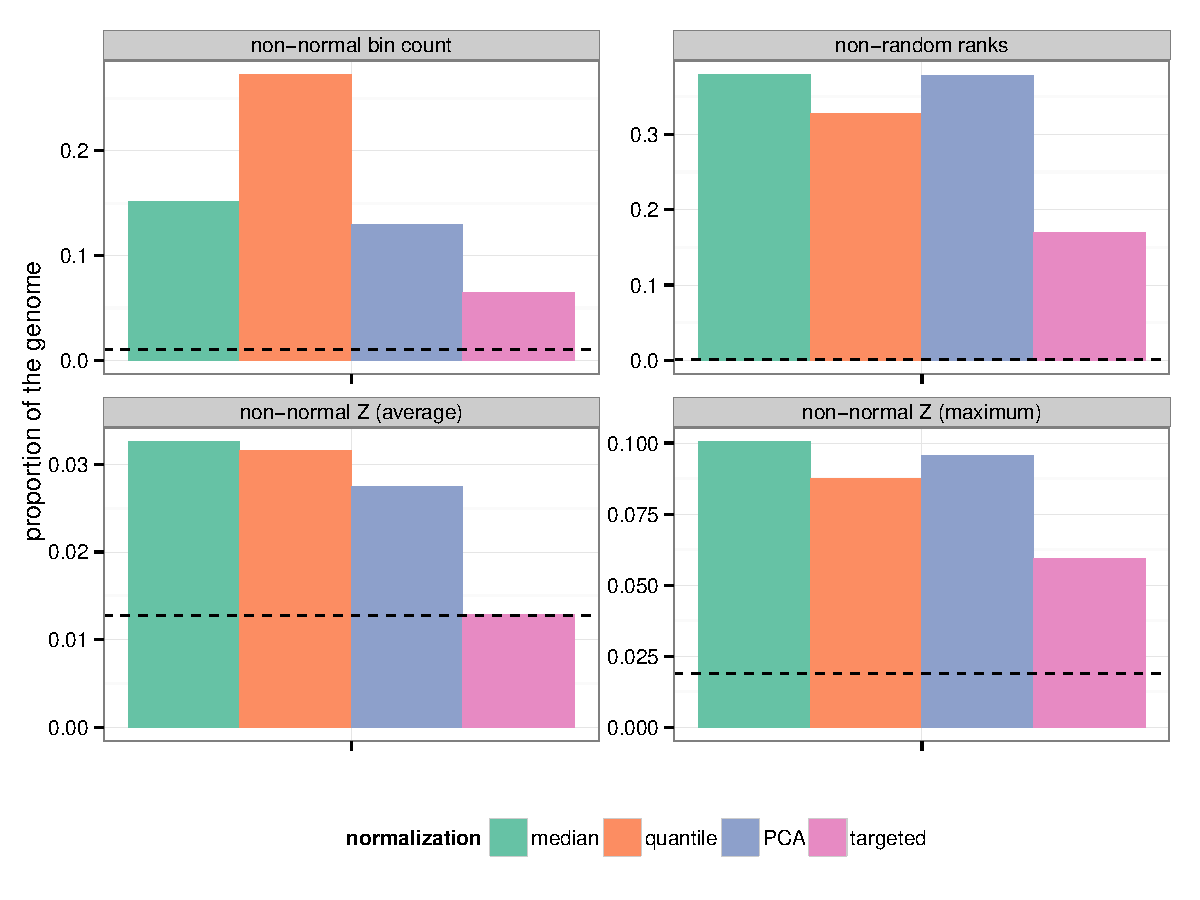
\includegraphics[width=\linewidth,page=1]{figures/cagekid-5kbp-normComparison.pdf}
    \caption{}
    \label{fig:normComp}
  \end{subfigure}
  \caption[Comparison of different normalization approaches.]{{\bf Comparison of different normalization approaches.} {\small a) For each normalization approach, the sample with the least normal Z-score distribution is shown. b) After targeted normalization, a lower proportion of the genome looks problematic for the analysis. Fewer bins have non-normal bin counts (top-left), the sample ranks are more random suggesting less sample-specific bias (top-right), and Z-scores fit better a Normal distribution on average (bottom-left) and in the worst sample (bottom-right). The dotted line is computed from simulated bin counts. }}
\end{figure}

\begin{figure}[htp]
  \centering
  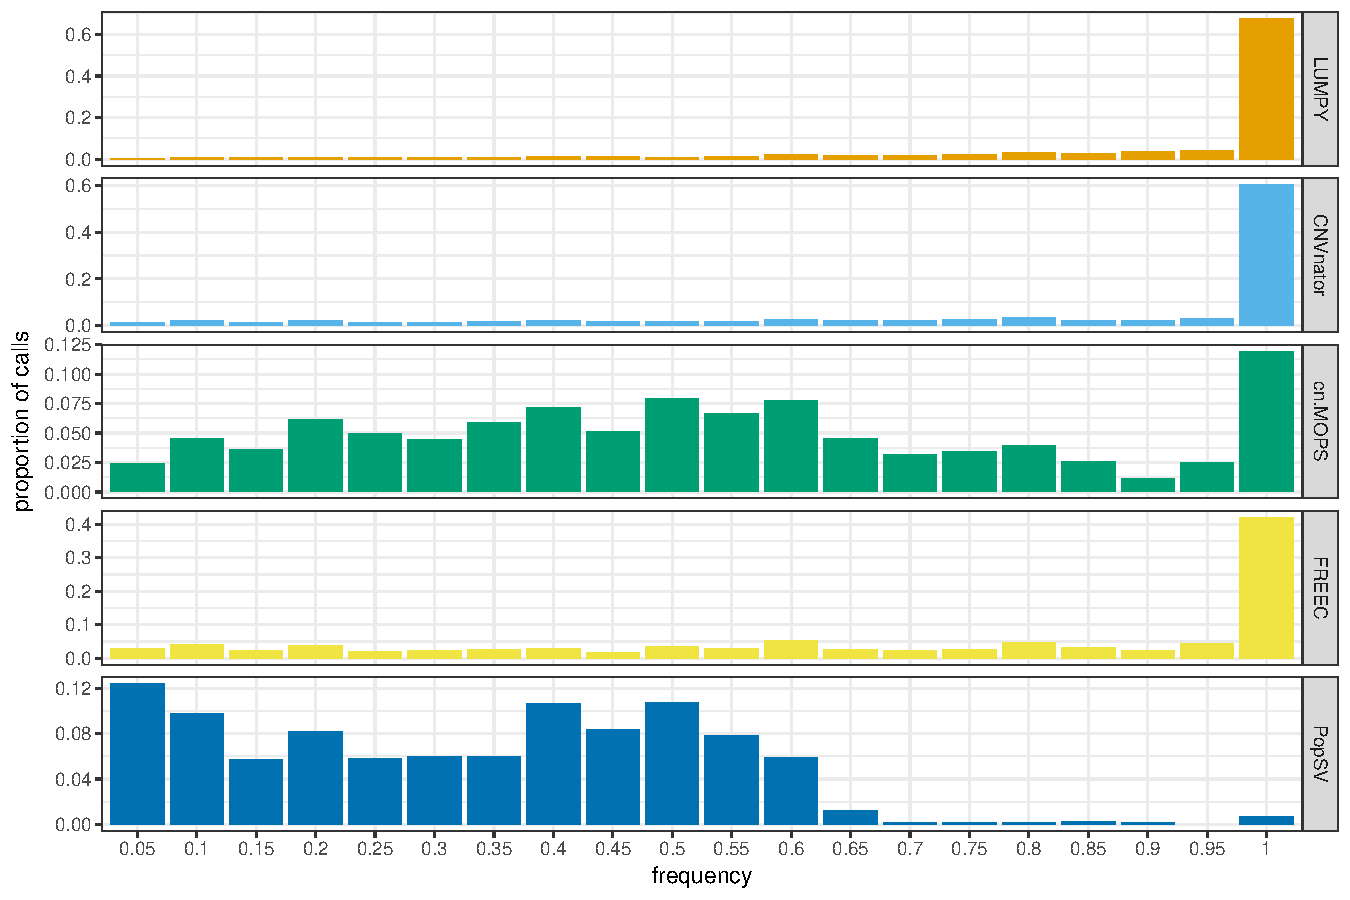
\includegraphics[width=\linewidth, page=1]{figures/twin-benchmark.pdf}
  \caption[Frequency of calls in an average sample from the Twin study.]{{\bf Frequency of calls in an average sample from the Twin study.} {\small The bars show the proportion of calls in an average samples (y-axis), grouped by the frequency of the call in the dataset (x-axis), for different methods.}}
  \label{fig:freqmeth}
\end{figure}

\begin{figure}[htp]
  \centering
  \includegraphics[width=.8\linewidth, page=2]{figures/twin-benchmark.pdf}
  \caption[CNV clustering and twin pedigree.]{{\bf CNV clustering and twin pedigree.} {\small The hierarchical cluster tree from the CNV calls is cut at different levels ({\it x-axis}), cluster groups are compared to the known pedigree using the Rand index ({\it y-axis}). Different clustering linkage criteria ({\it point style}) are used and the one showing the best Rand index is highlighted by the line.}}
  \label{fig:twinclust}
\end{figure}

\begin{figure}[htp]
  \centering
  \includegraphics[width=.8\linewidth, page=3]{figures/twin-benchmark.pdf}
  \caption[Replication in twins for different significance thresholds]{{\bf Replication in twins for different significance thresholds.} {\small Each point represents the number of replicated calls per sample (average across samples) and the proportion of replicated calls per sample. The vertical error bar shows the variation of the replication rate across the samples. The points and lines were computed by filtering calls at different significance levels (q-value for {\sf PopSV}, number of supporting reads for {\sf LUMPY} and eval1/eval2 for {\sf CNVnator}, see \nameref{sec:suppmat:epipopsv}).}}
  \label{fig:twinconcsig}
\end{figure}

\begin{figure}[htp]
  \centering
  \includegraphics[width=.9\linewidth, page=4]{figures/twin-benchmark.pdf}
  \caption[Calls found by several methods]{{\bf Calls found by several methods.} {\small Focusing on calls found by at least two methods, the heatmap shows the proportion of calls from one method (x-axis) that were also found by another (y-axis) on average per sample.}}
  \label{fig:twincallcomp}
\end{figure}

\begin{figure}[htp]
  \centering
  \begin{subfigure}{.48\textwidth}
    \includegraphics[width=\linewidth, page=3]{figures/cagekid-benchmark.pdf}
    \caption{}
  \end{subfigure}
  \begin{subfigure}{.48\textwidth}
    \includegraphics[width=\linewidth, page=2]{figures/cagekid-benchmark.pdf}
    \caption{}
  \end{subfigure}
  \begin{subfigure}{.48\textwidth}
    \includegraphics[width=\linewidth, page=4]{figures/cagekid-benchmark.pdf}
    \caption{}
  \end{subfigure}
  \begin{subfigure}{.48\textwidth}
    \includegraphics[width=\linewidth, page=5]{figures/cagekid-benchmark.pdf}
    \caption{}
  \end{subfigure}
  \caption[Benchmark across paired normal/tumor in CageKid]{{\bf Benchmark across paired normal/tumor in CageKid.} {\small Number (a) and proportion (b) of germline calls replicated in the paired tumor in CageKid. c) Number and proportion of replicated calls when filtering calls at different significance levels. d) Focusing on calls found by at least two methods, the color shows the proportion of calls from one method (x-axis) that were also found by another (y-axis) on average per sample. }}
  \label{fig:ckconc}
\end{figure}

\begin{figure}[htp]
  \centering
  \begin{subfigure}{.48\textwidth}
    \includegraphics[width=\linewidth, page=2]{figures/twin-binSizeComp.pdf}
    \caption{}
    \label{fig:size:spec}
  \end{subfigure}
  \begin{subfigure}{.48\textwidth}
    \includegraphics[width=\linewidth, page=4]{figures/twin-binSizeComp.pdf}
    \caption{}
    \label{fig:size:zdel}
  \end{subfigure}

  \begin{subfigure}{.48\textwidth}
    \includegraphics[width=\linewidth, page=3]{figures/twin-binSizeComp.pdf}
    \caption{}
    \label{fig:size:zdup}
  \end{subfigure}
  \begin{subfigure}{.48\textwidth}
    \includegraphics[width=\linewidth,page=6]{figures/twin-binSizeComp.pdf}
    \caption{}
    \label{fig:size:sens}
  \end{subfigure}
  \caption[Comparison of {\sf PopSV} results using different bin sizes.]{{\bf Comparison of {\sf PopSV} results using different bin sizes.} {\small a) 5 Kbp calls of different sizes (x-axis) are split according to the proportion of the call supported by 500 bp calls. The Z-score of 500 bp bins in 5 Kbp calls is consistent with the call for deletion b) and duplication c) signal. 5 Kbp calls with lower significance (e.g. single-bin calls) are less supported by 500 bp calls (a) but their Z-scores are in the consistent direction (b,c) although not always significant enough to be called. d) Proportion of 500 bp calls of different sizes (x-axis) overlapping a 5 Kbp call.}}
  \label{fig:compsize}
\end{figure}

\begin{figure}[htp]
  \centering
  \includegraphics[width=.9\linewidth]{figures/wgs-array-sizeComp.pdf}
  \caption[CNV size in our cohort and array-based studies.]{{\bf CNV size in our cohort and four array-based studies.} {\small The bars show the average number of CNVs called in a sample in the different cohorts. {\it Redon 2006}\cite{Redon2006} and {\it Itsara 2009}\cite{Itsara2009} are population studies using technology similar to previous epilepsy studies. {\it Addis 2016}\cite{Addis2016} is a recent study of large CNVs in absence epilepsy. {\it Conrad 2010}\cite{Conrad2010} is a population study that used multiple arrays to increase its resolution. }}
  \label{fig:arraysize}
\end{figure}

\begin{figure}[htp]
  \centering
  \includegraphics[width=.9\linewidth, page=2]{figures/epilepsy-enrichmentPatterns.pdf}
  \caption[Exonic enrichment significance.]{{\bf Exonic enrichment significance.} {\small The grey violin plot represents the difference in fold-enrichment between patients and controls across 10,000 permutations where the patient/control labels had been shuffled. The red point represents the observed difference between patients and controls (Fig. \ref{fig:exenr}).}}
  \label{fig:exenrsig}
\end{figure}


\begin{figure}[htp]
  \centering
  \begin{subfigure}[b]{.7\textwidth}
    \includegraphics[width=\linewidth,page=3]{figures/epilepsy-enrichmentPatterns.pdf}
    \caption{}
    \label{fig:epiexpriv}
  \end{subfigure}

  \begin{subfigure}[b]{.49\textwidth}
    \includegraphics[width=\linewidth,page=5]{figures/epilepsy-enrichmentPatterns.pdf}
    \caption{}
    \label{fig:epiexpriv2}
  \end{subfigure}
  \begin{subfigure}[b]{.49\textwidth}
    \includegraphics[width=\linewidth,page=4]{figures/epilepsy-enrichmentPatterns.pdf}
    \caption{}
  \end{subfigure}
  \caption[Rare exonic CNVs are less private in the epilepsy cohort.]{{\bf Rare exonic CNVs are less private in the epilepsy cohort.} {\small Proportion of rare exonic CNVs (y-axis) seen in X or more individuals (x-axis). The ribbon shows the 5\%-95\% confidence interval. In b), only French-Canadians individuals were analyzed and we down-sampled the epilepsy cohort to match the sample size of the French-Canadians controls. In c), the top 20 samples with the most non-private rare exonic SVs were removed. }}
\end{figure}

\begin{figure}[htp]
  \centering
  \begin{subfigure}[b]{.7\textwidth}
    \includegraphics[width=\linewidth,page=10]{figures/epilepsy-enrichmentPatterns.pdf}
    \caption{}
    \label{fig:epigenesize}
  \end{subfigure}
  \begin{subfigure}[b]{.7\textwidth}
    \includegraphics[width=\linewidth,page=12]{figures/epilepsy-enrichmentPatterns.pdf}
    \caption{}
    \label{fig:epicnvex}
  \end{subfigure}

  \caption[Enrichment in epilepsy genes.]{{\bf Enrichment in epilepsy genes.} {\small a) Epilepsy genes (red) are genes known to be associated with epilepsy. The control genes (dotted blue) are random genes selected so that the size distribution is similar to the sizes of genes hit by CNVs (plain blue). b) In three different datasets (color), genes hit by rare deletion (top) or duplications (bottom) at different frequency thresholds (x-axis) were tested for enrichment in epilepsy genes (y-axis, point-size).}}
\end{figure}

\begin{figure}[ht]
  \centering
  \begin{subfigure}[b]{.7\textwidth}
    \includegraphics[width=\linewidth, page=6]{figures/epilepsy-enrichmentPatterns.pdf}
    \caption{Rare CNVs}
    \label{fig:epidistnc}
  \end{subfigure}
  \begin{subfigure}[b]{.7\textwidth}
    \includegraphics[width=\linewidth, page=7]{figures/epilepsy-enrichmentPatterns.pdf}
    \caption{Rare deletions}
    \label{fig:epidistncdel}
  \end{subfigure}
  \caption[Rare non-coding CNVs near epilepsy genes.]{{\bf Rare non-coding CNVs near epilepsy genes.} {\small The graphs show the cumulative number of individuals (y-axis) with a rare non-coding variants located at X Kbp or less (x-axis) from the exonic sequence of a known epilepsy gene. The controls were down-sampled to the sample size of the epilepsy cohort. The ribbon shows the 5\%/95\% confidence interval. In a), deletions and duplications were considered; in b), only deletions were used.}}
\end{figure}

\begin{figure}[htp]
  \centering
  \begin{subfigure}[b]{\textwidth}
    \fbox{\includegraphics[width=\linewidth]{figures/ncdel-GABRD-ucscBrowser.pdf}}
    \caption{}
    \label{fig:ncepiexdel}
  \end{subfigure}
  \begin{subfigure}[b]{\textwidth}
    \fbox{\includegraphics[width=\linewidth]{figures/ncDup-CSNK1E-ucscBrowser.pdf}}
    \caption{}
    \label{fig:ncepiex1}
  \end{subfigure}
  \begin{subfigure}[b]{\textwidth}
    \fbox{\includegraphics[width=\linewidth]{figures/ncDel-FAM63B-ucscBrowser-eQTLs.pdf}}
    \caption{}
    \label{fig:ncepiex2}
  \end{subfigure}

  \caption[Non-coding CNVs with putative pathogenicity.]{{\bf Non-coding CNVs with putative pathogenicity.} {\small a) 2.7 Kbp deletion in an epilepsy patient, never seen in controls or CNV databases. Three other epilepsy patients have a rare non-coding deletions located at less than 200 Kbp from the {\it GABRD} gene. b) 8.8 Kbp duplication in two epilepsy patients, never seen in controls or CNV databases and overlapping a regulatory region associated with {\it CSNK1E}. c) 6.5 Kbp deletion of an ultra-conserved regions downstream of {\it FAM63B}. Two expression QTLs for this gene are highlighted with arrows.}}
\end{figure}

\begin{figure}[ht]
  \includegraphics[width=\linewidth, page=9]{figures/epilepsy-enrichmentPatterns.pdf}
  \caption[The enrichment in rare non-coding CNVs overlapping functional regions increases close to epilepsy genes.]{{\bf The enrichment in rare non-coding CNVs overlapping functional regions increases close to epilepsy genes.} {\small The graph shows the log odds ratio of having a rare non-coding CNV located at X Kbp or less (x-axis) from the exonic sequence of a known epilepsy gene. The y-axis shows the log odds ratio between epilepsy patients and controls. The controls were down-sampled to the sample size of the epilepsy cohort. We used CNVs overlapping regions functionally associated with the epilepsy gene (eQTL or promoter-associated DNase site).}}
  \label{fig:epidistncfunOR}
\end{figure}

\begin{figure}[htp]
  \centering
  \includegraphics[width=\linewidth]{figures/CHD2-deletedExon.png}
  \caption[Small deletion of exon 13 in {\it CHD2}.]{{\bf Small deletion of exon 13 in {\it CHD2}.} {\small Abnormal mapping of the read pairs highlighted in red support the deletion detected by {\sf PopSV} using the read coverage. The deletion region is highlighted in orange.}}
  \label{fig:chd213}
\end{figure}

\begin{figure}[htp]
  \centering
  \begin{subfigure}[b]{.49\textwidth}
    \includegraphics[width=\linewidth, page=1]{figures/PopSV-cohortSize.pdf}
    \caption{}
  \end{subfigure}
  \begin{subfigure}[b]{.49\textwidth}
    \includegraphics[width=\linewidth, page=3]{figures/PopSV-cohortSize.pdf}
    \caption{}
  \end{subfigure}
  \caption[Reference cohort size and CNV detection quality.]{{\bf Reference cohort size and CNV detection quality.} {\small {\sf PopSV} was run on the Twins study using 10, 20, 30 or 45 samples as reference (color). In a), the y-axis shows how many calls from the down-sampled run were found in the original 45-refs run. The x-axis represents the FDR threshold (lower threshold being more stringent). b) Replication in twins. For different cohort sizes and FDR thresholds, the number (x-axis) and proportion (y-axis) of calls replicated in the other twin is shown. In both graphs, the lines represents the median per sample and the ribbon the minimum/maximum values.}}
  \label{fig:cohortsize}
\end{figure}



%%%% 
%%%% 
%%%%%% FIGURES FOR SUPP MAT
%%%% 
%%%% 
\clearpage

\begin{figure}[htp]
  \centering
  \includegraphics[width=.8\textwidth]{figures/TargetNorm.pdf}
  \caption[Targeted normalization.]{{\bf Targeted normalization.} {\small The coverage across the reference samples (blue) in the bin to normalize is used to find supporting bins across the genome. These supporting bins only are used to compute the normalization factor. The same supporting bins will be used to normalize the bin count in a test sample (red).}}
  \label{fig:targetNorm}
\end{figure}

\clearpage

\section*{Supplementary Information}
\label{sec:suppmat:epipopsv}

\subsection*{Epilepsy patients and sequencing}

\paragraph{Ethics and patients recruitment}
CENet is a Genome Canada and Genome Qu\'ebec funded initiative that aims to bring personalized medicine in the treatment of epilepsy. Patients were recruited through two main recruitment sites at the Centre Hospitalier Universitaire de Montr\'eal (CHUM) and the Sick Kids Hospital in Toronto.
This study was approved by the Research Ethics Board at the Sick Kids Hospital (REB number \verb!1000033784!) and the ethics committee at the Centre Hospitalier Universitaire de Montr\'eal (project number \verb!2003-1394,ND02.058-BSP(CA)!).
Before their inclusion in this study, patients had to give written informed consents. The main cohort of this study was constituted of 198 unrelated patients with various types of epilepsy; 85 males and 113 females. The mean age at onset of the disease for our cohort was 9.2 ($\pm$6.7). Supplementary Table \ref{tab:clinical} presents a detailed description of the clinical features for the various individuals recruited in this study. DNA was extracted from blood DNA exclusively.
301 unrelated healthy parents of other probands from CENet were also included in this study and used as controls.

\paragraph{Libraries preparation and sequencing}
gDNA was cleaned up using ZR-96 DNA Clean \& Concentrator\textsuperscript{TM}-5 Kit (Zymo) prior to being quantified using the Quant-iT\textsuperscript{TM} PicoGreen\textregistered\ dsDNA Assay Kit (Life Technologies) and its integrity assessed on agarose gels.
Libraries were generated using the TruSeq DNA PCR-Free Library Preparation Kit (Illumina) according to the manufacturer's recommendations.
Libraries were quantified using the Quant-iT\textsuperscript{TM} PicoGreen\textregistered\ dsDNA Assay Kit (Life Technologies) and the Kapa Illumina GA with Revised Primers-SYBR Fast Universal kit (Kapa Biosystems).
Average size fragment was determined using a LabChip GX (PerkinElmer) instrument.

The libraries were first denatured in 0.05N NaOH and then were diluted to 8pM using HT1 buffer.
The clustering was done on a Illumina cBot and the flowcell was run on a HiSeq 2500 for 2x125 cycles (paired-end mode) using v4 chemistry and following the manufacturer's instructions.
A phiX library was used as a control and mixed with libraries at 1\% level.
The Illumina control software was HCS 2.2.58, the real-time analysis program was RTA v. 1.18.64. Program bcl2fastq v1.8.4 was then used to demultiplex samples and generate fastq reads.
The average coverage was 37.6x $\pm$ 5.6x.
The filtered reads were aligned to reference Homo\_sapiens assembly b37.
Each readset was aligned using {\sf BWA}\citep{Li2010} which creates a Binary Alignment Map file (.bam).
Then, all readset BAM files from the same sample are merged into a single global BAM file using Picard.
Insertion and deletion realignment was performed on regions where multiple base mismatches were preferred over INDELs by the aligner since it appears to be less costly for the algorithm.
Such regions were found to introduce false positive variant calls which may be filtered out by realigning those regions properly.
Once local regions were realigned, the read mate coordinates of the aligned reads needed to be recalculated since the reads are realigned at positions that differ from their original alignment.
Fixing the read mate positions is performed using Picard.
Aligned reads were marked as duplicates if they have the same 5' alignment positions (for both mates in the case of paired-end reads).
All but the best pair (based on alignment score) were marked as a duplicate in the \verb!.bam! file.
Duplicates reads were excluded in the subsequent analysis. Marking duplicates was performed using Picard.

\subsection*{Testing for technical bias in WGS}
To investigate the bias in read depth (RD), we first fragmented the genome in non-overlapping bins of 5 Kbp. The number of properly mapped reads was used as RD measure, defined as read pairs with correct orientation and insert size, and a mapping quality of 30 (Phred score) or more. In each sample, GC bias was corrected by fitting a Loess model between the bin's RD and the bin's GC content. Using this model, the correction factor for each bin was estimated from its GC content. Bins with extreme coverage were identified when deviating from the median coverage by more than 3 standard deviation. After these conventional intra-sample corrections, RD across the different samples were combined and quantile normalized. At that point the different samples had the same global RD distribution and no bins with extreme coverage or GC bias. Two control RD datasets were constructed to represent our expectation when no bias is present. One was derived from the original RD by shuffling the bins' RD in each sample. In the second, RD was simulated from a Normal distribution with mean and variance fitted to the real distribution. Simulation or shuffling ensures that no region-specific or sample-specific bias remains. To investigate region-specific bias, we computed the mean and standard deviation of the RD in each bin across the different samples. The same was performed in the control datasets. If there is no bias, the distribution of these estimators should be similar in the original, shuffled and simulated RD. Next, to investigate experiment-specific bias, we retrieved which sample had the highest coverage in each bin. Then we computed, for each sample, the proportion of the genome where it had the highest coverage. If no bias was present, e.g. in the shuffled and simulated datasets, each sample should have the highest coverage in 100/N \% of the genome (with N the number of samples). If an experiment was more affected by technical bias, it would be more often extreme. The same analysis was performed monitoring the lowest coverage.

The same analysis was ran after correcting the coverage in the Twin dataset using the {\sf QDNAseq} pipeline\cite{Scheinin2014}.
The reads were counted in 5 Kbp bins using the function \verb!binReadCounts!.
GC bias and mappability were corrected using the following functions (with default parameters): \verb!applyFilters!, \verb!estimateCorrection!, \verb!correctBins!, \verb!normalizeBins!, \verb!smoothOutlierBins!.

\subsection*{{\sf PopSV}}

\paragraph{Binning and coverage measure}
The genome is fragmented in non-overlapping consecutive bins of fixed size (5 Kbp). In each bin and each sample the number of reads that overlap the bin and are properly mapped are counted to get a measure of coverage. Read pairs with correct orientation and insert size, and a mapping quality of 30 (Phred score) or more are considered properly mapped. The bin counts were then corrected for GC bias. In each sample, a LOESS model was fitted between the bin's count and bin's GC content. A normalization factor was then defined for each bin from its GC content.

\paragraph{Constructing the set of reference samples}
In the epilepsy study and the Twins dataset we used all the samples as reference. In the renal cancer dataset we used the normal samples as reference. For each dataset, a Principal Component Analysis (PCA) was performed across samples on the counts normalized globally (median/variance adjusted). The resulting first two principal components are used to verify the homogeneity of the reference samples.
In the presence of extreme outliers or clear sub-groups, a more cautious analysis would be recommended. For example, outliers can remain in the set of reference samples but flagged as they might potentially harbor more false calls later. Independent analysis in each of the identified sub-group is also a solution, especially when the same samples are to be used as reference.
Although our three datasets showed different levels of homogeneity, we did not need to exclude samples or split the analysis. The effect of weak outlier samples was either corrected by the normalization step or integrated in the population-view. Moreover, the principal components were used to select one control sample from the final set of reference samples. This sample is used in the normalization step as a baseline to normalize other samples against. We picked the sample closest to the centroid of the reference samples in the Principal Component space.

\paragraph{Normalization}
Although uniformity of the coverage across the genome is not required for our approach, RD values must be comparable across samples. When a particular region of the genome is tested, sample specific variation of technical origin must be minimized. This is done through a normalization step.
Naive global normalization approaches like the Trimmed-Mean M(TMM) or quantile normalization have been first implemented and tested. The TMM normalization robustly aligns the mean RD value in the samples. Quantile normalization forces the RD distribution to be exactly the same in each sample. After witnessing the presence of uncharacterized sample-specific variation, we implemented a more suited normalization.
Targeted normalization uses information across the set of reference samples to identify similar bins across the genome and normalize their counts separately (Fig. \ref{fig:targetNorm}). For each bin, the top 1000 bins with similar coverage patterns across the reference samples are used to normalize the coverage of the bin. TMM normalization is used on these top 1000 bins to derive the correct normalization factor for the bin to normalize. Similarity between two bins is measured using Pearson correlation between the counts across the reference samples. Hence, the top 1000 bins are most similar in term of relative coverage across the samples to the coverage in the bin to normalize. If some bias is present in some samples, the top 1000 bins should also harbor this bias. Hence, other regions with similar bias patterns are used to correct for it. In this targeted approach, each genomic region is normalized independently. The 1000 supporting bins are saved and used to normalized new samples (e.g. case sample). Although computationally expensive, it ensures that all bins are normalized with the same effort. In contrast, global normalization or even PCA-based approaches corrects for the most common or spread bias, but a subset of regions with specific bias might not be corrected.
In order to compare the performance of the different normalization approaches we computed a set of quality metrics. The normalized RD will need to be suited for testing abnormal pattern across samples: under the null hypothesis, i.e. for normal bins, the RD should be relatively normally distributed and the samples rank should vary randomly from one bin to the other. The first metric is the proportion of bins with non-normal RD across the samples. Shapiro test was performed on each bin and a P-value lower than 0.01 defined non-normal RD. Then, the randomness of the sample ranks was tested by comparing the RD of each sample a region with the median across all samples. In regions of 100 consecutive bins, we counted how many times the RD in a sample was higher than the median across sample. If the ranks are random, this value should be around 0.5. The probability under the Binomial distribution is computed for each sample and corrected for multiple testing using Bonferroni correction. If any sample has an adjusted P-value lower than 0.05, we consider that the region has non-random ranks. The resulting QC metric is simply the proportion of regions with non-random sample ranks. This QC is specifically testing how much sample-specific bias remains. The remaining QC metrics look at the Z-score distribution in each sample. The proportion of non-normal Z-scores is computed by comparing the density curves of the Z-scores and simulated Normal Z-scores. We compute the proportion of the area under the density curve that does not overlap the Normal density curve. This estimate of the proportion of non-normal Z-scores is computed in each sample. The final metrics are the average and maximum across the samples.

\paragraph{Abnormal RD test and Z-score computation}
The test is based on Z-scores computed for each bin, corrected afterward for multiple testing. The Z-score represents how different the read count in the tested sample is from the reference samples. It is simply: $z=\frac{BC_t^b-mean(BC_{ref}^b)}{sd(BC_{ref}^b)}$ where $BC_t^b$ is the bin count, i.e. the number of reads, in bin $b$ and sample $t$.
Inevitably some samples are hosting common CNVs. We observed that just a couple of samples hosting a CNVs could be enough to bias the standard deviation used in the score computation and mask these CNVs in the coming tests. In many cases the RD signal was clearly showing several groups of samples with proportional read counts. To improve the Z-score computation in those regions, a simple approach was used: the samples were stringently clustered using their RD and the group with higher number of samples was chosen as reference and used to compute the mean and standard deviation for the Z-score computation. In practice, this clustering affects only bins with clear clusters but would remove just a few or no samples in most situations. Furthermore, a median-based estimator was used for the standard deviation as it is less sensitive to outlier removal. A trimmed mean was also preferred over normal mean for its robustness to outliers.

\paragraph{Significance and multiple testing correction}
The Z-scores for all the bins of a sample are pooled and significance is estimated. Under the null hypothesis of normally distributed read counts, the Z-scores should also follow a normal distribution. For multiple testing correction, the Z-score empirical distribution is used to fit a normal and estimate the P-value and Q-value of each test. This step is performed using fdrtool R package.
By default, the null distribution fitting for P-value computation assumes that only a low proportion of bins violates the null hypothesis. In aberrant genomes, e.g. in tumor samples, it is often an unrealistic assumption. We devised a new strategy to set the proportion of the empirical distribution, later used to estimate the null distribution variance. Here the null Z-score distribution is assumed to be centered on 0 and its variance is estimated by trimming the tails of the empirical distribution. To find a correct trimming factor, an iterative approach started from a low trimming factor and increased its value until reaching a plateau for the variance estimator. Indeed, once the plateau is reached, additional trimming does not change the estimated variance because there is no more abnormal Z-scores, only the central part of the null distribution. Samples with an important proportion of abnormal genome, e.g. tumor samples, showed more appropriate fit.
Of note, the P-values for positive Z-scores (duplication) and negative Z-scores (deletion) are estimated separately. Thus, imbalance in the deletion to duplication ratio, or large aberration that lead to asymmetrical Z-score distribution does not affect the P-value estimation. Multiple testing correction is performed after pooling all the P-values.

\paragraph{Segmentation, copy number estimation and other metrics}
Following the significance estimation, consecutive bins with abnormal coverage are merged into a call.
Consecutive or nearby abnormal bins (e.g. one bin size apart) are merged into one variant if in the same direction (deletion or duplication).
In {\sf PopSV}'s R package, the P-values can also be segmented using circular binary segmentation\cite{Seshan2017}.

In addition to the Z-score, P-value, Q-value and number of bins of each call, {\sf PopSV} retrieves the average coverage in the reference samples and the fold change in the sample tested. The copy number is estimated by dividing the coverage in a region by the average coverage across the reference samples, multiplied by 2 (as diploidy is expected). In our bin setting, the estimation is correct if the bin spans completely the variant. For this reason we trust the copy number estimate for calls spanning 3 or more consecutive bins, as it is computed using the middle bin(s) which completely span the variant. In other cases we expect the copy number estimate to be under-estimated.
All this additional information can be used to order or retrieve high confidence calls. For examples, several consecutive bins or a copy number estimate around an integer value increases our confidence in a call. In our benchmark, we used the entire set of calls.

\subsection*{Validation and benchmark of {\sf PopSV}}

We compared {\sf PopSV} to {\sf FREEC}\citep{Boeva2011}, {\sf CNVnator}\citep{Abyzov2011} and {\sf cn.MOPS}\citep{Klambauer2012}, three popular RD methods that can be applied to WGS datasets to identify CNVs. {\sf FREEC} segments the RD values of a sample using a LASSO-based algorithm while {\sf CNVnator} uses a mean-shift technique inspired from image processing. {\sf cn.MOPS} considers simultaneously several samples and detects copy number variation using a Poisson model and a Bayesian approach. We also ran {\sf LUMPY}\citep{Layer2012} which uses an orthogonal mapping signal: the insert size, orientation and split mapping of paired reads.

{\sf FREEC} and {\sf CNVnator} were run on each sample separately, starting from the BAM file. {\sf FREEC} internally corrects the RD for GC and mappability bias. In order to compare its performance across the entire genome, the minimum telocentromeric distance was set to 0. The remaining parameters were set to default. Of note an additional run with slightly looser parameter ('breakPointThreshold=0.6') was performed to get a larger set of calls used in some parts of the in silico validation analysis to deal with borderline significant calls. {\sf CNVnator} also corrects internally for GC bias. We used default parameters. For the analysis using higher confidence calls, we used calls with either 'eval1' or 'eval2' lower than 10-5 (instead of the default 0.05).
{\sf cn.MOPS} was run on the same GC-corrected bin counts used for {\sf PopSV}. All the samples are analyzed jointly. Of note an additional run with slightly looser parameter ('upperThreshold=0.32' and 'lowerThreshold=-0.42') was performed to get a larger set of calls used in some parts of the in silico validation analysis to deal with borderline significant calls.
For {\sf LUMPY}, the discordant reads were extracted from the BAMs using the recommended commands. Split-reads were obtained by running {\sf YAHA}\citep{Faust2012} with default parameters. All the CNVs (deletions and duplications) larger than 300 bp were kept for the upcoming analysis. Calls with 5 or more supporting reads were considered high-confidence.

First, we compared the frequency at which a region is affected by a CNV using the calls from the different methods. In order to investigate how many systematic calls are present in a typical run, we compare the frequency distributions on average per sample. In figure \ref{fig:freqmeth}, the bars represents the average proportion of a sample's calls in each frequency range.

Then, the samples were clustered using the CNV calls. The distance between two samples A and B is defined as : $1-2 \frac{|VAB|}{(|VA|+|VB|)}$ where VA represents the variants found in sample A, VAB the variants found in both A and B, and |V| the cumulative size of the variants. Hence, the similarity between two samples is represented by the amount of sequence called in both divided by the average amount of sequence called. This distance is used for hierarchical clustering of the samples. Different linkage criteria (``average'', ``complete'' and ``Ward'') were used for the exploration. In our dendograms we used the ``average'' linkage criterion. The same clustering was performed using only calls in regions with extremely low coverage (reference average <10 reads).

To assess the performance of each method, we measured the number of CNVs identified in each twin that were also found in the matching twin. In order to avoid missing calls with borderline significance, we used slightly less confident calls for the second twin. We removed calls present in more than 50\% of the samples to ensure that systematic errors were not biasing our replication estimates. Hence, a replicated call is most likely true as it is present in a minority of samples but consistently in the twin pair. Even if we removed systematic calls, the most frequent calls in the cohort are more likely to look replicated by chance, compared to rare calls. To normalize for this effect, we use the frequency distribution to compute the number of replicated calls expected by chance. In practice the null concordance for each call is simulated by a Bernoulli distribution of parameter the frequency of the call. This number of replicated calls by chance is subtracted to the original number of replicated calls to give an adjusted measure of sensitivity. Although we do not know the true number of variant, this number of replicated calls is used to compare the different methods.
When possible, the low-quality calls were also gradually filtered to explore the effect on the replication metrics.
For {\sf CNVnator}, we used the minimum of the eval1 and eval2 columns, with lower values corresponding to higher quality calls.
For {\sf LUMPY}, the number of supporting reads was used.
For {\sf PopSV}, we filtered calls based on adjusted P-values.

In addition to their replication, we compared which regions were called by several methods.
For each of the calls found in less than 50\% of the samples, we overlapped the region with calls from other methods in the same sample.
If calls from another method overlapped we considered the call shared and saved which methods shared the call.
To focus on on high quality calls we considered calls found by at least two methods and computed the proportion of calls from one method found by each of the other methods.
This metric captures how much each method recovers high-quality calls from a second method.


\paragraph{Concordance between different bin sizes}
We compared calls using small bins (500 bp) and calls using larger bins (5 Kbp). In theory, calls from the 5 Kbp analysis should be supported by many 500 bp calls. We also expect large stretches of 500 bp calls to be detected in the 5 Kbp analysis. This comparison is informative as it explores the quality of the calls, the size of detectable events and the resolution for different bin sizes. First we counted how many small bin calls supported any large bin call. These metrics were separated according to the size of the large bin call. Overall, we find that 5 Kbp calls are well supported by 500 bp calls, with only 14\% of the 5 Kbp bins not supported by any 500 bp bin (Fig. \ref{fig:size:spec}). To investigate large bin calls with no supporting small bin call, we display the average Z-scores in the small bins overlapping large bin calls to test if the lack of support is due to lower confidence or real discordancy between the different runs. If the Z-scores in the small bins deviates from 0 in the correct direction, we conclude that they support the large bin call. Even for these unsupported 5 Kbp calls, we find that the 500 bp bins RD was consistently enriched (or depleted) although not enough to be called with confidence (Fig. \ref{fig:size:zdel} and \ref{fig:size:zdup}). This is expected given the higher background noise in the 500 bp analysis that will reduce the power to call these variants. Next, we looked at the proportion of 500 bp calls, grouped by size, that were found in the 5 Kbp calls. More specifically, we grouped them by size to verify that large enough small bin calls are present in the large bin calls. This analysis is used to both test the sensitivity of {\sf PopSV} with a particular bin size, and its resolution to variants smaller than the bin size. Indeed, this framework allow us to ask questions such as: how much of the variants spanning only half a bin are detected? We find that the concordance gradually increases until the 500 bp calls reach 5 Kbp in size where the concordance rises to nearly 100\% (Fig. \ref{fig:size:sens}). This suggests that {\sf PopSV} is able to detect approximately 75\% of the events as large as half its bin size, and almost all events larger than its bin size. As expected, only a small proportion of the small 500 bp calls overlap 5 Kbp calls and they likely corresponds to fragmented larger calls. Considering the trade-off between bin size and noise, this suggests running {\sf PopSV} with a few bin sizes to better capture variants of different sizes.

\subsection*{CNV detection in the CENet cohorts}
CNVs were called using {\sf PopSV} using 5 Kbp bins and all the samples from both the epilepsy and control cohorts as reference.
We annotated the frequency of the CNVs using germline CNV calls from the Twin and cancer datasets (internal database) as well as four public CNV databases:

\begin{itemize}
\item CNVs from Phase 1 of the 1000 Genomes Project as identified by {\sf GenomeSTRiP}\citep{Handsaker2015}.
\item SV from the 1000 Genomes Project phase 3\citep{Sudmant2015a}.
\item Genome of Netherlands\citep{Francioli2014}.
\item CNVs from the Simons Genome Diversity Project\citep{Sudmant2015}.
\end{itemize}

CNVs were annotated with the maximum frequency in the databases.
For each CNV to annotate, any overlapping CNV in the CNV databases were considered.
This is a stringent criterion that ensures that the entire regions of a rare CNV, for example, is never affected by common CNVs in the databases. 
Hence, a rare CNV is defined as present in less than 1\% of the samples in each of the five CNV databases.

To test for a difference in deletion/duplication ratio among rare CNVs, we compared the numbers of rare deletions and duplications in the epilepsy patients and controls using a $\chi^2$ test.
The same test was performed after downsampling the controls to the sample size of the epilepsy cohort.

\subsection*{CNV enrichment in exonic region and around epilepsy genes}

\paragraph{Enrichment in exons}
For each cohort, we retrieved the CNV catalog by merging CNV that are recurrent in multiple samples.
Hence, the CNV catalog represents all the different CNVs found in each cohort.
To control for the population size, we sub-sampled 150 samples in each cohort a hundred times.
For each sub-sampling and each cohort, control regions are selected to fit the size distribution of the CNV catalog and the overlap with centromere, telomeres and assembly gaps (details in the next section).

Then, we computed the proportion of CNV and control regions that overlap an exon.
The fold-enrichment is the ratio of these proportions and represents how much more/less of the CNVs overlap an exon compared to the control regions.
The boxplot in Fig. \ref{fig:exenr} shows the distribution of the 100 sub-sampling in each cohort.


To test if the difference observed between the cohort is significant, the {\it cohort} labels were permuted 10,000 times and the difference in median across the 100 sub-sampling was saved.
The resulting P-value was computed as $\frac{1+d}{1+N}$ where $d$ is the number of times the permuted difference was greater or equal to the observed difference, and $N$ is the number of permutations.

The same analysis was repeated for exons from genes with a probability of loss-of-function intolerance\citep{Lek2016} higher than 0.9.
These genes were called {\it LoF intolerant genes} in Fig. \ref{fig:exenr}.
Small (< 50Kbp) and large (>50 Kbp) CNVs were analyzed separately.
The analysis was repeated using rare CNVs only.


\paragraph{Selecting control regions}
The control regions must have the same size distribution as the regions they are derived from (e.g. CNVs in a CNV catalog).
We also controlled for the overlap with centromere, telomeres and assembly gaps (CTGs) to avoid selecting control regions in assembly gaps where no CNV or annotation is available.
To select control regions, thousands of bases were first randomly chosen in the genome.
The distance between each base and the nearest CTG was then computed.
At this point, selecting a region of a specific size and with specific overlap profile can be done by randomly choosing as center one of the bases that fit the profile:

\begin{equation}
  \left\{b,  O_{CTG}(d_{CTG}^b - \frac{S_r}{2}) < 0\right\}  
\end{equation}

\noindent with $O_{CTG}$ equals 1 if the original region overlaps with a CTG, -1 if not; $d_{CTG}^b$ is the distance between base $b$ and the nearest CTG; and $S_r$ is the size of the original region.
For each input region, a control region was selected and had by construction the exact same size and overlap profile.


\paragraph{Recurrence of rare exonic CNVs}
In each cohort, we retrieved the CNV catalog of rare (<1\% in all 5 public datasets) exonic CNVs.
We annotated each CNV with its recurrence in the cohort.
We then evaluated the proportion of the CNVs in the catalog that are private (i.e. seen in only one sample), or seen in X samples or more.
This cumulative proportion of CNVs is shown in Fig. \ref{fig:epiexpriv}.
The control cohort was down-sampled a thousand times to the same sample size as the epilepsy cohort.
These down-sampling provided a confidence interval (ribbon in Fig. \ref{fig:epiexpriv}) and an empirical P-value.

We performed the same analysis after removing the top 20 samples with the most non-private rare exonic CNVs (Fig. \ref{fig:epiexpriv2}).
With this analysis, we tried to remove the potential effect of a few extreme samples.

We also repeated the analysis using only French-Canadians individuals, to ensure that the observed differences are not caused by rare population-specific variants (Fig. \ref{fig:epiexpriv2}).


\paragraph{CNVs and epilepsy genes}
We used the list of genes associated with epilepsy from the EpilepsyGene resource\citep{Ran2015} which consists of 154 genes strongly associated with epilepsy.
For a particular set of CNV we count how many of the genes hit are known epilepsy genes.
We noticed that the epilepsy genes tend to be large, and genes hit by CNVs also (Fig. \ref{fig:epigenesize}).
This could lead to a spurious association so we also performed a permutation approach that controls for the size of the genes.
To control for the gene size of epilepsy genes and CNV-hit genes, we randomly selected genes with sizes similar to the genes hit by CNVs and evaluated how many of these were epilepsy genes.
After ten thousand samplings, we computed an empirical P-value.
The permutation P-value was computed as $\frac{1+d}{1+N}$ where $d$ is the number of times the number of epilepsy genes in the random set of genes was greater or equal to the one in genes hit by CNVs, and $N$ is the number of permutations.
Using this sampling approach we tested different sets of CNVs: deletion or duplications of different frequencies in the epilepsy cohort, control individuals and samples from the twin study.

To investigate rare non-coding CNV close to known epilepsy genes, we counted how many patients have such a CNV at different distance thresholds.
For example, how many patients had a rare non-coding CNV at 10 Kbp of an epilepsy gene's exon or closer.
We compared this cumulative distribution to the control cohort, after down-sampling it to the sample size of the epilepsy cohort.
Down-sampling was also used to produce a confidence interval, represented by the ribbon in Fig. \ref{fig:epidistncfun}).
This analysis was repeated using deletions only.
Each epilepsy gene was also tested for an excess of rare non-coding deletions in patients versus controls using a Fisher test.

In order to retrieve non-coding CNV that might have a functional impact, we downloaded eQTLs associated with the epilepsy genes, as well as DNase 1 hypersensitive sites associated with the promoter of epilepsy genes.
The eQTLs are provided by the GTEx project\citep{Ardlie2015}.
Pairs of associated DNase 1 hypersensitive sites and associated genes\citep{Maurano2012} were downloaded at \url{http://www.uwencode.org/proj/Science_Maurano_Humbert_et_al/data/genomewideCorrs_above0.7_promoterPlusMinus500kb_withGeneNames_35celltypeCategories.bed8.gz}.

A Kolmogorov-Smirnov test was used to compare the distance distributions in epilepsy patients versus controls.
We also computed the odds ratio of having such a CNV for different distance thresholds between epilepsy patients and controls.
For a distance $d$, we computed:

$$ OR = \frac{S_{patient}^{CNV}}{S_{control}^{CNV}} / \frac{S_{patient}^{noCNV}}{S_{control}^{noCNV}} $$

where $S_{patient}^{CNV}$ is the number of patients with a rare non-coding CNV overlapping a functional region and located at $d$ bp or less from the exon of a known epilepsy gene.


%%% Local Variables:
%%% mode: latex
%%% TeX-master: "../main"
%%% End:


\clearpage

\section*{Appendix D}
\addcontentsline{toc}{section}{Appendix D: Supplementary Materials from Chapter \ref{chap:rep}}
\label{append:rep}
Supplementary material for chapter \ref{chap:rep} and its corresponding manuscript: {\bf Human copy number variants are enriched in regions of low mappability}.

%% Create counter for supp figs ("S1" etc)
\setcounter{figure}{0}
\renewcommand{\thefigure}{S\ref{chap:rep}.\arabic{figure}}
\setcounter{table}{0}
\renewcommand{\thetable}{S\ref{chap:rep}.\arabic{table}}

\section*{Supplementary Tables}


\begin{table}[htp]
  \centering
  \resizebox{\textwidth}{!}{
    \begin{tabular}{|c|r|r|r|l|c|c|}
      \hline
      Validated & Chr. & Start     & End       & Class        & Left PCR primer                & Right PCR primer               \\
      \hline
      V      & 3    & 6649794   & 6654897   & large CN 0   & CCTTAGTATTTCAGTGGTTTCTGTAGGTAT & ATAAATATCAGTGCTCAACTTGGACTT    \\
      V      & 5    & 127407030 & 127411341 & large CN 0   & TATTCATATTAACCTATCCTCACAGAAAGA & TTTTTAAGAGATTTGAACTAAAATTCCAC  \\
      V      & 3    & 5535139   & 5539535   & large CN 0   & TACTTTTTGAATTTGTAAATTTCCTTTGTA & GAAATCAGAAAATCAAGATCATACTGAAG  \\
      V      & 1    & 116229111 & 116233162 & large CN 0   & GTGTTACAGAATTAGTTTTACTGAGTGGTC & ATCTATAAAGAACTTTTTCCAAATAAACCA \\
      V      & 1    & 158961082 & 158966958 & large CN 1   & GTAGAATGAGCTGTGTTATGAGATGGT    & ATGACTTTCTATTGTTTGAAATGTAGTGAC \\
      V      & 15   & 26748887  & 26752614  & large CN 1   & CAATTTATCTATCAAGTTATTTCACGGTAG & AGTGAGATTTCATTTTAAGCTTGTCTTC   \\
      V      & 6    & 33937344  & 33942846  & large CN 1   & ACATTGTAGCCTGATGACCTTGTTC      & TGTGTTCTGAGGTTTACTTTATAATCTAGG \\
      V      & 12   & 82095501  & 82099389  & large CN 1   & ACCTATAACTAAGTGTAGCTGCTGTAACTG & TCAGTAAAAATGATTACTACAGTGGAAAAT \\
      V      & 5    & 8255604   & 8260914   & large CN 1   & TGAACATACATTCATACACACATAATACAA & TACATCACTGAACAAACCTCTATAGTCATA \\
      V      & 20   & 7398397   & 7403743   & large CN 1   & AATAAACATTCTCTATAAACCCTAAAATGG & CTTTGTACCATATTTCATAAACGTAGAGTC \\
      V      & 18   & 40053822  & 40057873  & large CN 1   & TAACTTTCTTTTCTAAAGCTTTTGGAGTAT & GTGAATTAAGATTCAATGTCTCTGCTAATA \\
      V      & 16   & 48904951  & 48906510  & small CN 0   & TCTTATTTATTTTGACAGTCCTTTACTCTG & AGATAATCAACTCTTTGTTTATTCTTTCAG \\
      V      & 2    & 241086647 & 241087801 & small CN 0   & ATCAACATTTAGCCAGTGTTGTCTTAG    & GTCTCTTGTGCTCTATCTTTGGCTT      \\
      V      & 13   & 110221621 & 110222631 & small CN 0   & ACCTCAGGAGAACTACTTCATACATTTCTA & GTATGAAAAACACTCATGGATATCATTTCT \\
      V      & 11   & 60571017  & 60572170  & small CN 0   & AATGTTGAAGTGTGTCTTTCTGTAATATCT & GTGTTTTGTGTCGCTATTTGTTTAGTA    \\
      V      & 5    & 166402295 & 166404219 & small CN 0   & TCACTTTATTCATAACATTTCAGTGTAGAG & GATCATATGCTTAAAATGCTAATGAGG    \\
      N     & 3    & 160126422 & 160127288 & small CN 1   & TAAGATACAAGAAATAGAGATAACACTGGG & TCTGAACACTTATTTTAAGAAAATGAAAAA \\
      N     & 17   & 10612674  & 10613775  & small CN 1   & AATTTAGCAGTCTCTTACATTTCTTCTACC & TCTCTTCTATAAAAATAAATGGCTAAAAGC \\
      V      & 10   & 70253713  & 70255155  & small CN 1   & AATAAAATCAAAGGTGATATTACTGACAGA & ATATACTCTTTTAACTTTTGACCATTTTGG \\
      V      & 8    & 53700635  & 53702050  & small CN 1   & TAAGGAAAATTTAGTATAGTCTGGACCTGT & ATGGAAATATATCTCTGATGGGTGAC     \\
      % N     & 6    & 26636844  & 26637539  & low coverage & GTACATAGATTCTCACCCACAATTAAATC  & CTTCTTCAACATCAGACAGTACACATT    \\
      % N     & 13   & 78236245  & 78238105  & low coverage & GTCAGTCTGGTTCTTTTCTGTCAAG      & ACTTTAGTAAAATTGTTATTTAGTCCCAGG \\
      % V      & 1    & 248546279 & 248548008 & low coverage & CTATCTTTCTTACCATTTAATATCTGCCTT & AGACTTCATTTAGGAAAGTGAGAAATACAC \\
      \hline
    \end{tabular}
  }
  \caption[Experimental validation results.]{{\bf Experimental validation results.} {\small Location of the validated (V) and non-validated (N) CNVs for different classes. The last two columns show the primer sequences used for PCR amplification.}}
  \label{tab:pcr}
\end{table}

\begin{table}[htp]
  \centering
  \resizebox{\textwidth}{!}{
    \begin{tabular}{|r|r|r|l|r|r|l|l|l|}
      \hline
      Chr. & Start & End & CN & PCR product size & PCR product size when deletion & Validated & Gel & Sanger Sequencing\\
      \hline
      14 & 40098378 & 40100213 & 0 & 2586 & 751 & Yes & Different bands & Yes: confirmed\\
      \hline
      5 & 85559864 & 85564846 & 1.05 & 5690 & 708 & Yes & Different bands & Yes: confirmed\\
      \hline
      6 & 14299746 & 14299801 & 0.79 & 755 & 700 & Yes & Double bands & No\\
      \hline
      7 & 153000055 & 153000246 & 1.76 & 1137 & 946 & Yes & Double bands & Yes: confirmed\\
      \hline
      4 & 96401034 & 96401460 & 1.13 & 745 & 319 & Yes & Double bands & No\\
      \hline
      16 & 34230052 & 34230512 & 1 & 1139 & 679 & Yes & Double bands & No\\
      \hline
      16 & 8688137 & 8689592 & 1.02 & 2121 & 666 & Yes & Double bands & Yes: confirmed\\
      \hline
      2 & 12018994 & 12022932 & 1.02 & 4291 & 353 & Yes & Double bands & Yes: confirmed\\
      \hline
      3 & 121051576 & 121060845 & 1.14 & 9485 & 216 & Yes & Double bands & No\\
      \hline
      3 & 54433855 & 54433912 & 0 & 952 & 895 & Yes & One band & Yes: insertion\\
      \hline
      2 & 151031059 & 151038246 & 1.11 & 7485 & 298 & Yes & Small band only & No\\
      \hline
      9 & 45462450 & 45462522 & 1.1 & 530 & 458 & No & One band & No\\
      \hline
      7 & 63233184 & 63233261 & 1.33 & 390 & 313 & No & One band & Yes: nothing\\
      \hline
      9 & 106371251 & 106371330 & 1.28 & 484 & 405 & No & One band & No\\
      \hline
      16 & 20466400 & 20466487 & 1.27 & 393 & 306 & No & One band & No\\
      \hline
      5 & 85559864 & 85564842 & 0.78 & 5690 & 712 & No & One band & No\\
      \hline
      10 & 65703860 & 65708900 & 1.64 & 5430 & 390 & No & One band & No\\
      \hline
      7 & 159117395 & 159122761 & 1.09 & 5909 & 543 & No & One band & No\\
      \hline
      2 & 83066824 & 83068234 & 0.57 & 2097 & 687 & NA & No amplification & No\\
      \hline
      13 & 35996202 & 35996254 & 1.13 & 546 & 494 & NA & Non-specific & No\\
      \hline
      4 & 159799983 & 159801372 & 1.03 & 2313 & 924 & NA & Non-specific & Yes: not clear\\
      \hline
      7 & 52963172 & 52964911 & 1.48 & 2316 & 577 & NA & Non-specific & No\\
      \hline
      10 & 69323932 & 69326507 & 1.62 & 2795 & 220 & NA & Non-specific & Yes: not clear\\
      \hline
      6 & 58618198 & 58624080 & 1.04 & 6518 & 636 & NA & Non-specific & No\\
      \hline
    \end{tabular}
  }
  \caption[Experimental validation in low-coverage regions.]{{\bf Experimental validation in low-coverage regions.} {\small The result of the PCR validation was either concordant with {\sf PopSV} call (Yes), discordant (No) or inconclusive (NA). In some cases, Sanger sequencing was performed. The {\it CN} column is the estimated copy-number of the deleted allele.}}
  \label{tab:pcr2}
\end{table}

\begin{table}[htp]
  \centering
  \resizebox{.6\textwidth}{!}{
    \begin{tabular}{|r|r|r|}
      \multicolumn{3}{l}{{\bf Homozygous deletion}} \\
      \hline
       deletion support & reference support & number of calls \\
      \hline
      0   & 0   & 11     \\
      0   & 1   & 1      \\
      1   & 0   & 1      \\
      2   & 0   & 12     \\
      \hline
      \multicolumn{3}{l}{{\bf Heterozygous deletion}} \\
      \hline
       deletion support & reference support & number of calls \\
      \hline
      0   & 0   & 18     \\
      0   & 1   & 10     \\
      0   & 2   & 7      \\
      1   & 0   & 6      \\
      1   & 1   & 4      \\
      1   & 2   & 4      \\
      2   & 0   & 10     \\
      2   & 1   & 3      \\
      \hline
    \end{tabular}
  }
  \caption[Investigating low-mappability deletion calls with two CEPH12878 assemblies.]{{\bf Investigating low-mappability deletion calls with two CEPH12878 assemblies.} {\small The first two columns represent the number of assemblies (0, 1 or 2) supporting the deleted allele or the reference allele. The third column shows the number of {\sf PopSV} calls in each category.}}
  \label{tab:cephAss}
\end{table}

\begin{table}[htp]
  \centering
  \resizebox{\textwidth}{!}{
    \begin{tabular}{|l|r|rrr|r|r|rr|}
      \hline
      \multirow{2}{*}{CNV catalog} & \multirow{2}{*}{Samples} & \multicolumn{3}{c|}{Variants} & \multirow{2}{*}{Avg Size (Kbp)} & Proportion & \multicolumn{2}{c|}{Affected genome (Mbp)} \\
      
                                          &       & Total  & \multicolumn{2}{c|}{Per sample} &           & $<$3 Kbp & Total & Per sample    \\
      \hline
                                          &       &        & {\it WG}                        & {\it ELC} &          &       &        &      \\
      1000GP                              & 2,504 & 41,979 & 1,024.44                        & 2.22      & 6.00     & 0.68  & 580.03 & 6.14 \\
      {\it ~~deletion}                    &       & 36,102 & 975.32                          & 2.21      & 4.67     & 0.72  & 342.97 & 4.56 \\
      {\it ~~duplication}                 &       & 8,503  & 48.26                           & 0.00      & 32.54    & 0.00  & 331.48 & 1.57 \\
      \hline                                
      GoNL                                & 750   & 9,592  & 1,048.14                        & 0.63      & 2.93     & 0.81  & 65.30  & 3.07 \\
      {\it ~~deletion}                    &       & 9,009  & 1,013.35                        & 0.63      & 2.36     & 0.82  & 34.79  & 2.39 \\
      {\it ~~duplication}                 &       & 528    & 21.11                           & 0.00      & 29.19    & 0.15  & 30.63  & 0.62 \\
      \hline                                
      Handsaker 2015 ({\sf Genome STRiP}) & 847   & 8,657  & 212.03                          & 1.88      & 27.80    & 0.00  & 196.57 & 5.89 \\
      {\it ~~deletion}                    &       & 5,961  & 145.78                          & 0.56      & 21.64    & 0.00  & 108.03 & 3.15 \\
      {\it ~~duplication}                 &       & 3,469  & 66.26                           & 1.32      & 41.35    & 0.00  & 118.28 & 2.74 \\
      \hline                                
      Chiang 2017 ({\sf Genome STRiP})    & 148   & 7,932  & 828.49                          & 9.23      & 6.35     & 0.42  & 73.20  & 5.26 \\
      \hline
    \end{tabular}
  }
    \caption[Properties of events in public CNV catalogs]{{\bf Properties of events in public CNV catalogs.} {\small Deletions, duplications and CNVs from four public catalogs. Variants with high frequency ($>80\%$), variants on the chromosome X, and variants smaller than 300 bp were removed in order to compare with {\sf PopSV}'s numbers (Table \ref{tab:res}). WG: whole genome; ELC: extremely low-coverage regions. The {\it Total} number of variants is the total number after collapsing recurrent variants. {\it Affected genome} represents the amount of the reference genome that overlaps at least one CNV.}}
  \label{tab:1kgp}
\end{table}


\begin{table}[htp]
  \centering
  \resizebox{.8\textwidth}{!}{
    \begin{tabular}{|l|l|l|l|l|}
      \cline{1-2}\cline{4-5}              
      Novel region          & OMIM gene && Novel region           & OMIM gene \\
      \cline{1-2}\cline{4-5}              
      1:25730001-25736000   & RHCE      && 9:136418001-136420000  & ADAMTSL2  \\
      \cline{1-2}\cline{4-5}              
      1:161640001-161645000 & FCGR2B    && 10:64130001-64135000   & ZNF365    \\
      \cline{1-2}\cline{4-5}              
      1:207705001-207715000 & CR1       && 10:101595001-101600000 & ABCC2     \\
      \cline{4-5}                         
      1:207725001-207745000 & CR1       && 10:135380001-135383500 & SYCE1     \\
      \cline{1-2}\cline{4-5}                                       
      5:68845001-68886000   & OCLN      && 11:320001-325000       & IFITM3    \\
      \cline{1-2}\cline{4-5}                                      
      5:69360001-69365000   & SMN2      && 12:52683001-52685000   & KRT81     \\
      \cline{4-5}                         
      5:69373001-69374000   & SMN2      && 12:52696001-52696500   & KRT86     \\
      \cline{1-2}\cline{4-5}                                       
      5:70165001-70222000   & SMN1      && 15:32454001-32460000   & CHRNA7    \\
      5:70242001-70242500   & SMN1      && 15:32464001-32464500   & CHRNA7    \\
      \cline{4-5}                         
      5:70246501-70258000   & SMN1      && 15:43902501-43903000   & STRC      \\
      \cline{1-2}
      6:29905001-29910000   & HLA-A     && 15:43910001-43910500   & STRC      \\
      \cline{1-2}\cline{4-5}                                       
      6:31960001-31975000   & C4A       && 16:21760001-21765000   & OTOA      \\
      \cline{1-2}\cline{4-5}                                       
      6:31995001-31995500   & C4B       && 17:34504001-34545000   & CCL3L3    \\
      \cline{1-2}\cline{4-5}                                       
      6:32522001-32560000   & HLA-DRB1  && 19:11535001-11540000   & CCDC151   \\
      \cline{1-2}\cline{4-5}                                       
      6:32590001-32602000   & HLA-DQA1  && 19:41340001-41350000   & CYP2A6    \\
      \cline{1-2}\cline{4-5}                                       
      6:32628501-32629000   & HLA-DQB1  && 22:18660001-18765000   & USP18     \\
      \cline{4-5}                                       
      6:32630001-32634000   & HLA-DQB1  && 22:18904501-18905500   & PRODH     \\
      \cline{1-2}
      7:39052001-39055500   & POU6F2    && 22:18909001-18909500   & PRODH     \\
      \cline{1-2}\cline{4-5}                                       
      7:74195001-74200000   & NCF1      &       \multicolumn{3}{c}{}        \\
      \cline{1-2}
    \end{tabular}
  }
  \caption[OMIM genes overlapping novel CNV regions of low-mappability]{{\bf OMIM genes overlapping novel CNV regions of low-mappability} {\small Novel CNV regions are polymorphic in more than 1\% of the individuals across the three cohorts but absent from the 1000GP SV catalog\cite{Sudmant2015a}. OMIM genes are genes associated with a disease or phenotype in the OMIM Morbid Map (Online Mendelian Inheritance in Man; \url{http://omim.org/}).}}
  \label{tab:omimgenes}
\end{table}


\clearpage

\section*{Supplementary Figures}

\begin{figure}[htp]
  \centering
  \begin{subfigure}[b]{.48\textwidth}
    \includegraphics[width=\linewidth,page=2]{figures/wgs-map-coverage-cohorts.pdf}
    \caption{}
    \label{fig:mapcov}
  \end{subfigure}
  \begin{subfigure}[b]{.48\textwidth}
    \includegraphics[width=\linewidth,page=3]{figures/wgs-map-coverage-cohorts.pdf}
    \caption{}
    \label{fig:meancov}
  \end{subfigure}

  \begin{subfigure}[b]{.48\textwidth}
    \includegraphics[width=\linewidth,page=7]{figures/wgs-map-coverage-cohorts.pdf}
    \caption{}
    \label{fig:meancohort}
  \end{subfigure}
  \begin{subfigure}[b]{.48\textwidth}
    \includegraphics[width=\linewidth,page=8]{figures/wgs-map-coverage-cohorts.pdf}
    \caption{}
    \label{fig:sdcohort}
  \end{subfigure}

  \caption[Coverage, mappability and population-based measures]{{\bf Coverage, mappability and population-based measures.} {\small a-b) Read coverage in a sample (y-axis) versus mappability (a) or the inter-sample average coverage (b). c-d) Inter-sample mean (c) and standard deviation (d) were fitted against the mappability in each cohort separately. The tiles represent all cohorts pooled together.}}
\end{figure}

\begin{figure}[htp]
  \centering
  \begin{subfigure}[b]{.48\textwidth}
    \includegraphics[width=\linewidth,page=1]{figures/wgs-coverage-tracks-cagekid-gonl.pdf}
    \caption{}
  \end{subfigure}
  \begin{subfigure}[b]{.48\textwidth}
    \includegraphics[width=\linewidth,page=3]{figures/wgs-coverage-tracks-cagekid-gonl.pdf}
    \caption{}
  \end{subfigure}

  \caption[Average coverage in reference samples in the CageKid and GoNL datasets.]{{\bf Average coverage in reference samples in the CageKid (a) and GoNL (b) datasets.}}
  \label{fig:covclass2}
\end{figure}

\begin{figure}[htp]
  \includegraphics[width=\linewidth,page=5]{figures/replication-twins.pdf}
  \caption[Rand index between pedigree and CNV-based dendogram in low-coverage regions.]{{\bf Rand index between the pedigree information and the dendogram from CNV calls in low-coverage regions.} {\small The dendogram for CNV-based clustering was cut at different levels (x-axis) and the groups compared to the pedigree (family-level) with the Rand index (y-axis). For each method, the line highlights the best performance across three linkage criteria.}}
  \label{fig:randindex}
\end{figure}

\begin{figure}[htp]
  \includegraphics[width=\linewidth,page=2]{figures/replication-cagekid.pdf}
  \caption[{\sf PopSV}'s performance in low-mappability regions in CageKid dataset.]{{\bf {\sf PopSV}'s performance in low-mappability regions in CageKid dataset.} {\small Proportion and number of calls replicated in the paired tumor. The point shows the median value per sample, the error bars the 95\% confidence interval.}}
  \label{fig:replication:cagekid}
\end{figure}

\begin{figure}[htp]
  \includegraphics[width=\linewidth,page=2]{figures/PopSV-NA12878-assembly-lowMap.pdf}
  \caption[Distance to assembly gaps and supporting evidence from long-read sequencing in CEPH12878.]{{\bf Distance to assembly gaps and supporting evidence from long-read sequencing in CEPH12878.} {\small Deletions in low-mappability regions were grouped by their supporting evidence (y-axis and colors). {\it assemblies}: deletion observed in at least one of the two public assemblies. {\it PB-SV}: overlap with a structural variant called from the PacBio reads\cite{Pendleton2015}. {\it PB-reads}: deletion observed in the local assembly or consensus of the PacBio reads. Variants with no support are represented by the white boxplot.}}
  \label{fig:cephGap}
\end{figure}

\begin{figure}[htp]
  \centering
  \includegraphics[width=\linewidth,page=3]{figures/PopSV-catalog-overview.pdf}
  \caption[Overlap between {\sf PopSV} catalog and calls from Pendleton et al..]{{\bf Overlap between {\sf PopSV} catalog and calls from Pendleton et al..} {\small Recurrent calls were collapsed in each catalog (i.e {\sf PopSV} and the 1000 Genomes Project (1000GP)). The proportion of the collapsed calls overlapping calls from \citet{Pendleton2015} was computed. The fold-enrichment is produced by drawing control regions with similar size distribution as Pendleton's calls. {\it low-map}: calls in low-mappability regions; {\it ext. low-map}: calls in extremely low-mappability regions.}}
  \label{fig:pendcat}
\end{figure}

\begin{figure}[htp]
  \centering
  \includegraphics[width=\textwidth,page=1]{figures/PopSV-repeatEnr.pdf}
  \caption[Distance to a centromere, telomere or assembly gap.]{{\bf Distance to a centromere, telomere or assembly gap.} {\small The y-axis represents the cumulative proportion of the affected genome. The {\it expected} curve is computed from uniformly distributed genomic regions with matched size.}}
  \label{fig:ctgDist}
\end{figure}

\begin{figure}[htp]
  \centering
  \begin{subfigure}{.9\textwidth}
    \includegraphics[width=\textwidth,page=2]{figures/PopSV-repeatEnr-long.pdf}
    \caption{}
    \label{fig:repCont}
  \end{subfigure}
  
  \begin{subfigure}{.48\textwidth}
    \includegraphics[width=\textwidth,page=4]{figures/PopSV-repeatEnr.pdf}
    \caption{}
    \label{fig:repSat}
  \end{subfigure}
  \begin{subfigure}{.48\textwidth}
    \includegraphics[width=\textwidth,page=6]{figures/PopSV-repeatEnr.pdf}
    \caption{}
    \label{fig:repSR}
  \end{subfigure}
  \caption[CNVs enrichment after controlling for segmental duplication overlap and distance to CTG.]{{\bf CNVs enrichment after controlling for segmental duplication overlap and distance to CTG.} {\small Enrichment of CNVs in a) different genomic features, b) satellite families and c) simple repeats in the different cohorts (colors). Bars show the median fold enrichment across samples compared to control regions. The star represents significant enrichment from the logistic regression.}}
\end{figure}

\begin{figure}[htp]
  \centering
  \begin{subfigure}{.48\textwidth}
    \includegraphics[width=\textwidth,page=5]{figures/PopSV-repeatEnr.pdf}
    \caption{Satellites}
  \end{subfigure}
  \begin{subfigure}{.48\textwidth}
    \includegraphics[width=\textwidth,page=7]{figures/PopSV-repeatEnr.pdf}
    \caption{Simple repeats}
  \end{subfigure}

  \begin{subfigure}{.48\textwidth}
    \includegraphics[width=\textwidth,page=9]{figures/PopSV-repeatEnr.pdf}
    \caption{Transposable elements}
  \end{subfigure}
  \caption[Overlap between CNVs and repeats.]{{\bf Overlap between CNVs and repeats.} {\small The histograms represent the proportion of the CNV region that overlaps a) a satellite, b) a simple repeat or c) a transposable element, when they do overlap. The {\it expected} distribution is computed from the control regions used for the enrichment analysis.}}
  \label{fig:repeatOl}
\end{figure}

\begin{figure}[htp]
  \centering
  \begin{subfigure}{.7\textwidth}
    \includegraphics[width=\textwidth,page=4]{figures/example-L1PA-NAHR.pdf}
    \caption{}
  \end{subfigure}
  
  \begin{subfigure}{.7\textwidth}
    \includegraphics[width=\textwidth,page=1]{figures/example-L1PA-NAHR.pdf}
    \caption{}
  \end{subfigure}
  \caption[Polymorphism likely caused by non-homologous allelic recombination between L1PA repeats.]{{\bf Polymorphism likely caused by non-homologous allelic recombination between L1PA repeats.} {\small Examples of CNV likely caused by non-allelic homologous recombination between two L1PA3 repeats (a) or L1PA6 (b). The line and points represent the coverage of one sample with a duplication (a) or a deletion (b), highlighted in yellow; the violin plots represent the distribution of the coverage in the reference samples. }}
  \label{fig:l1pa}
\end{figure}


\begin{figure}[htp]
  \centering
  \includegraphics[width=\textwidth,page=6]{figures/PopSV-catalog-overview.pdf}
  \caption[Novel CNV regions and CNVs in other public catalogs]{{\bf Novel CNV regions and CNVs in other public catalogs.} {\small Cumulative proportion of the 3,455 novel regions (y-axis) that overlap CNVs in different public CNV catalogs (colour) depending on their frequency in the public catalog (x-axis). The labels highlight the proportion of novel regions that don't overlap any CNV in the corresponding public catalog. Novel regions were defined as overlapping a CNV in more than 1\% of the individuals but absent from the 1000GP catalog.}}
  \label{fig:novelcatfreq}
\end{figure}





\clearpage

\section*{Supplementary Information}
\label{sec:suppmat:reppopsv}

\section*{Data}
\label{sec:data}

\paragraph{Twin study}
All patients gave informed consent in written form to participate in the Quebec Study of Newborn Twins\cite{Boivin2013}. Ethic boards from the Centre de Recherche du CHUM, from the Université Laval and from the Montreal Neurological Institute approved this study. Sequencing was done on an Illumina HiSeq 2500 (paired-end mode, fragment length ~300 bp). The reads were aligned using a modified version of the Burrows-Wheeler Aligner ({\sf bwa} version 0.6.2-r126-tpx with threading enabled). The options were \verb!'bwa aln -t 12 -q 5'! and \verb!'bwa sampe -t 12'!.
The aligned reads are available on the European Nucleotide Archive under \href{https://www.ebi.ac.uk/ena/data/view/PRJEB8308}{ENA PRJEB8308}.
The 45 samples had an average sequencing depth of 40x (minimum 34x / maximum 57x).

\paragraph{Renal cell carcinoma}
WGS data from renal cell carcinoma is presented in details in the CageKid paper\cite{Scelo2014}.
In short, 95 pairs of normal/tumor tissues were sequenced using GAIIx and HiSeq2000 instruments.
Paired-end reads of size 100 bp totaled an average sequencing depth of 54x (minimum 26x / maximum 164x).
Reads were trimmed with {\sf FASTX-Toolkit} and mapped per lane with {\sf BWA} backtrack to the GRCh37 reference genome.
{\sf Picard} was used to adjust pairs coordinates, flag duplicates and merged lane.
Finally, realignment was done with {\sf GATK}.
Raw sequence data have been deposited in the European Genome-phenome Archive, under the accession code \href{https://www.ebi.ac.uk/ega/studies/EGAS00001000083}{EGAS00001000083}.

\paragraph{Genome of the Netherlands}
WGS data from the GoNL project is described in details in \citet{Francioli2014}. This data have been derived from different sample collections:
\begin{itemize}
\item The LifeLines Cohort Study (\url{http://www.lifelines.nl/}), supported by the Netherlands Organization of Scientific Research (NWO, grant 175.010.2007.006), the Dutch government's Economic Structure Enhancing Fund (FES), the Ministry of Economic Affairs, the Ministry of Education, Culture and Science, the Ministry for Health, Welfare and Sports, the Northern Netherlands Collaboration of Provinces (SNN), the Province of Groningen, the University Medical Center Groningen, the University of Groningen, the Dutch Kidney Foundation and Dutch Diabetes Research Foundation.
\item The EMC Ergo Study (\url{http://www.ergo-onderzoek.nl/wp/}).
\item The LUMC Longevity Study, supported by the Innovation-Oriented Research Program on Genomics (SenterNovem IGE01014 and IGE05007), the Centre for Medical Systems Biology and the National Institute for Healthy Ageing (Grant 05040202 and 05060810).
\item VU Netherlands Twin Register (\url{http://www.tweelingenregister.org/}).
\end{itemize}

In short, samples were sequenced on an Illumina HiSeq 2000 instrument (91-bp paired-end reads, 500-bp insert size).
We downloaded the aligned read sequences (BAM) for the 500 parents in the data set.
We further performed indel realignment using {\sf GATK} 3.2.2, adjusted pairs coordinates with {\sf Samtools} 0.1.19, marked duplicates with {\sf Picard} 1.118, and performed base recalibration ({\sf GATK} 3.2.2).
The average sequencing depth was 14x (minimum 9x / maximum 59x).

\paragraph{Genomic annotations} Gencode annotation (V19) was directly downloaded from the consortium FTP server at \url{ftp://ftp.sanger.ac.uk/pub/gencode/Gencode_human/release_19/gencode.v19.annotation.gtf.gz}.
Other genomic annotations were downloaded from the UCSC database\cite{Rosenbloom2015} server at \url{http://hgdownload.soe.ucsc.edu/goldenPath/hg19/database}.
The file names of the corresponding annotations are
\label{sec:genodata}

\medskip

\begin{tabular}{|l|l|}
  \hline
  Mappability                          & \verb!wgEncodeCrgMapabilityAlign100mer.bw! \\
  Cytogenetic bands                    & \verb!cytoBandIdeo.txt.gz!                 \\
  Centromere, telomere, assembly gap   & \verb!gap.txt.gz!                          \\
  Segmental duplication                & \verb!genomicSuperDups.txt.gz!             \\
  Simple repeat / Short Tandem Repeats & \verb!simpleRepeat.txt.gz!                 \\
  RepeatMasker                         & \verb!rmsk.txt.gz!                         \\
  \hline
\end{tabular}

\section*{Read count across the genome}

The genome was fragmented in non-overlapping bins of fixed size.
The number of properly mapped reads was used as a coverage measure, defined as read pairs with correct orientation and insert size, and a mapping quality of 30 (Phred score) or more.
In each sample, GC bias was corrected by fitting a LOESS model between the bin's coverage and the bin's GC content.
For each bin, the correction factor was computed as the mean coverage across all the bins divided by the predicted coverage from the LOESS model and the GC content of the bin.
We used a bin size of 5 Kbp for most of the analysis.
When specified, we used a smaller bin size of 500 bp.

\section*{RD and mappability estimates}

To investigate the bias in RD we used the read counts in 5 Kbp bins.
Bins with extremely high coverage were identified and removed when deviating from the median coverage by more than 5 standard deviation.
First the coverage of the 45 samples from the Twin study were combined and quantile normalized.
At that point the different samples had the same global coverage distribution and no bins with extreme coverage or GC bias.

The mappability track\cite{Derrien2012} was downloaded from UCSC\cite{Rosenbloom2015} \\(\verb!wgEncodeCrgMapabilityAlign100mer.bw!) and the average mappability was computed for each bin.
One sample was randomly selected and we compared its coverage with the mappability estimates.
We then computed the mean and standard deviation of the coverage in each bin across the other samples and compared it with the sample coverage.
We also compared the inter-sample average with the mappability estimates.

To compute Z-scores that integrates the observed coverage variation we used two approaches.
The first modeled the coverage metrics (average or standard deviation) using the mappability estimates and computed a Z-score from the predicted coverage and global standard deviation.
A generalized additive model was fitted using a cubic regression spline on the mappability estimates ({\sf mgcv} R package).
In the second approach, Z-scores were computed using the inter-sample average and standard deviation.
The normality of these two Z-score distributions were compared in term of excess kurtosis and skewness.
For the kurtosis and skewness computation, we removed outlier Z-scores with an absolute value greater than 10. These bins could be regions of CNV and would bias the estimates.
The Z-score distributions were also compared in bins from 10 different mappability intervals.

We repeated this analysis pooling 45 samples from each of the three datasets.
After quantile normalization, the inter-sample coverage mean and standard deviation were computed separately in each cohort and compared with the mappability estimates.

\section*{CNV detection with {\sf PopSV}}

\paragraph{Binning the genome}
We ran two separate analysis on the three datasets.
Bin sizes of 5 Kbp and 500 bp were used on the Twin study and renal cell carcinoma.
Because of its lower sequencing depth, the 500 bp run on GoNL gave only partial results.
More precisely, we observed a truncated distribution of the copy-number estimates, with most of the 1 and 3 copy number variants missing.
It means that at this resolution many one-copy variation cannot be differentiated from background noise.
For this reason we ran GoNL analysis using 2 Kbp and 5 Kbp bins.

\paragraph{Constructing the set of reference samples}
In each dataset we choose the reference samples as follows: in the renal cancer dataset from the normal samples, in the Twin study from all the samples, in GoNL from a subset of 200 samples (see below).
For each dataset, a Principal Component Analysis (PCA) was performed across samples on the counts normalized globally (median/variance adjusted).
The resulting first two principal components are used to verify the homogeneity of the reference samples.
Although our three datasets showed different levels of homogeneity, we didn't need to exclude samples or split the analysis.
The effect of weak outlier samples was either corrected by the normalization step or integrated in the population-view.

In GoNL, we decided to use only 200 of the 500 samples as reference.
They were selected to span a maximum of the space defined by the principal components.
In contrast to random selection, this ensures that weak outliers are included in the final set of reference samples, hence maximizing the technical variation integrated in the population-view.

Moreover, the principal components were used to select one control sample from the final set of reference samples.
This sample is used in the normalization step as a baseline to normalize other samples against.
We picked the sample closest to the centroid of the reference samples in the Principal Component space.

\paragraph{CNV calling}
After targeted normalization the coverage in each sample is compared to the coverage in the reference samples.
A Z-score is computed and translated into a P-value that is then corrected for multiple testing.
Consecutive bins with significant excess or lack of reads are merged and returned as potential duplication or deletion.
Copy number estimates are derived from the coverage across the bin and the average coverage across the reference samples.
However, it is important to note that the definition of a variant is different from other methods.
Here a variant is defined by the major allele in the population rather than the reference genome state.
Most of the genome is in a diploid state compared to the reference genome and sufficiently covered by sequencing reads that the copy number state can be correctly estimated by {\sf PopSV}'s population-based approach.
However, highly polymorphic variants are called relative to the major allele in the population and additional efforts are required to assess the copy number state.
Variants in extremely low-mappability regions are also difficult to fully characterize and might be caused by rare insertion in the reference genome or complex alleles.
Nonetheless, {\sf PopSV} can efficiently detect the presence of CNV in any situation.
More details are available in the method paper\cite{Monlong2018}.

\paragraph{Coverage tracks}
For each run, we constructed coverage tracks based on the average coverage in the reference samples.
Bins where the reference samples had, on average, the expected coverage were classified as {\it expected coverage}.
Bins with a coverage lower than 4 standard deviation from the median were classified as {\it low-mappability}(or {\it low coverage}).
To ensure robustness, the standard deviation was derived from the Median Absolute Deviation.
We use regions with low coverage to define {\it low-mappability regions}, as the low coverage is a result of the lower mappability of a region.
Because the standard deviation is used, the number of regions classified as {\it low-mappability} is lower in datasets with more RD variance.

Eventually, we also defined {\it extremely low coverage} region which have an average coverage below 100.
This sub-class of {\it low coverage} region was used in a few analyses to highlight the most challenging regions.

Regions were annotated with the overlap with protein-coding genes and segmental duplications (see \nameref{sec:genodata}), and the distance to the nearest centromere, telomere or assembly gap.
Finally, we computed the number of protein-coding genes overlapping at least one low-coverage region.

\section*{Validation and benchmark}

\paragraph{Running {\sf FREEC}, {\sf CNVnator}, {\sf cn.MOPS} and {\sf LUMPY}}
{\sf FREEC}\cite{Boeva2011} segments the RD values of a sample using a LASSO-based algorithm.
It was run on each sample separately, starting from the BAM file, using the same bin sizes as for {\sf PopSV}.
{\sf FREEC} internally corrects the RD for GC and mappability bias.
In order to compare its performance in low-mappability region, the minimum {\it ``telocentromeric''} distance was set to 0.
The remaining parameters were set to default.
Of note an additional run with slightly looser parameter (\verb!breakPointThreshold=0.6!) was performed to get a larger set of calls used in some parts of the {\it in silico} validation analysis to deal with borderline significant calls.

{\sf CNVnator}\cite{Abyzov2011} uses a mean-shift technique inspired from image processing.
It was run on each sample separately, starting from the BAM file, using the same bin sizes as for {\sf PopSV}.
{\sf CNVnator} also corrects internally for GC bias and we used default parameters.
For the analysis using higher confidence calls, we used calls with either 'eval1' or 'eval2' lower than $10^{-5}$ (instead of the default 0.05).

{\sf cn.MOPS}\cite{Klambauer2012} considers simultaneously several samples and detects copy number variation using a Poisson model and a Bayesian approach.
It was run on the same GC-corrected bin counts used for {\sf PopSV}.
All the samples are analyzed jointly.
Of note an additional run with slightly looser parameter (\verb!upperThreshold=0.32! and \verb!lowerThreshold=-0.42!) was performed to get a larger set of calls used in some parts of the {\it in silico} validation analysis to deal with borderline significant calls.

{\sf LUMPY}\cite{Layer2012} which uses an orthogonal mapping signal: the insert size, orientation and split mapping of paired reads.
The discordant reads were extracted from the BAMs using the recommended commands.
Split-reads were obtained by running {\sf YAHA}\cite{Faust2012} with default parameters.
All the CNVs (deletions and duplications) larger than 300 bp were kept for the upcoming analysis.
\verb!BND! variants with both ends more than 300 bp apart in the same chromosome were also included as they could be CNVs lacking support to characterize their type properly.
Calls with 5 or more supporting reads were considered high-confidence.

\paragraph{Clustering samples from the Twin study}
A distance between two samples A and B was defined as : $1 - 2\frac{|R_A \cap R_B|}{|R_A| + |R_B|}$ where $R_A$ represents the regions called in sample A, $R_A \cap R_B$ the regions called in both A and B, and $|R|$ the cumulative size of the regions.
Hence, the similarity between two samples is represented by the amount of sequence found in both divided by the average amount of sequence called.
This distance is used for hierarchical clustering of the samples in the Twin dataset.
The clustering was performed using only calls in regions with extremely low coverage (reference average $\le$100 reads).
Different linkage criteria ({\it average}, {\it complete} and {\it Ward}) were used for the exploration.
In our dendograms we used the {\it average} linkage criterion.
The concordance between the clustering and the pedigree was estimated by the Rand index, grouping the samples per family.
For each method and linkage criteria, the Rand index was computed for every possible dendogram cut ({\it x}-axis in Figure \ref{fig:randindex}).

\section*{Experimental validation}
Experimental validation was performed on samples from the Twin study.
In a first validation batch, variants were randomly selected among both one-copy and two-copy deletions.
We selected both small ($\sim700$ bp) and large ($\sim4$ Kbp) variants in each class.
%%In addition, 3 deletions in low-mappability regions were also randomly selected and included.
The coverage at base pair resolution was visually inspected for each deletion and, when possible, the breakpoints were fine-tuned.
PCR primers were designed to target the whole deleted region.
We randomly selected 20 variants out of the variants for which we managed to design PCR primers.
We then performed long-range PCR followed by gel electrophoresis.
PCR was performed using 50 ng of DNA and the Phusion High-Fidelity DNA Polymerase from Thermo Fisher Scientific: 95 $^{\circ}$C 5 minutes followed by 35 cycles (95 $^{\circ}$C 30 seconds, 64 $^{\circ}$C 30 seconds, 72 $^{\circ}$C 45 seconds) and 72 $^{\circ}$C 10 minutes.
Either a 1\% or 1.8\% aragose gel was used, depending on the expected size of the amplified fragments.
We used a 1 Kb Plus DNA Ladder from Thermo Fisher Scientific.

The presence of a deletion was tested by comparing the size of the amplified fragment in affected and control samples.
If the affected sample showed a lower band than a control with a predicted 2 copies, the deletion was considered validated.
On the other hand if affected sample and controls had one similar band, the deletion was considered non-validated.
Of note, the validation rate might be under-estimated because visual prediction of the breakpoint is not always accurate.

We then randomly selected deletions overlapping low-mappability regions and detected in 6 samples or fewer.
We chose to test rare variants because they are likely enriched in false-positives.
Hence, this batch of validation represents the most challenging regions to call and validate, and enriched in false-positives.
Here we couldn't use the base-pair coverage to fine-tune the breakpoints because the low-mappability blurs any clear signal.
Instead, we retrieved the reads (and their pairs) mapping to the region and assembled them.
With this approach we could sometimes get a better breakpoint resolution and design PCR primers that would amplify the deleted region.
In addition to gel electrophoresis, the amplified DNA of some regions was sequenced using Sanger sequencing.
We randomly selected 17 variants out of the variants for which we managed to design PCR primers.

\section*{Analysis of CEPH12878}

\paragraph{Whole-Genome Sequencing data}
High coverage PCR-free Illumina WGS data for 30 samples, including CEPH12878, was downloaded from the 1000 Genomes Project\cite{Sudmant2015a}.
The ENA accession number is \href{http://www.ebi.ac.uk/ena/data/view/PRJNA260854}{PRJNA260854}.
The files are also available on the FTP server at \url{http://ftp.1000genomes.ebi.ac.uk/vol1/ftp/release/20130502/supporting/high_coverage_alignments/20141118_high_coverage.alignment.index}.
Although the sequencing depth is similar to the other datasets (average $\sim$53X), the reads are 250 bp long so the average number of reads per region is lower.
Because of the lower read coverage and sample size the CNV calls will be of slightly lower quality.
Nonetheless, {\sf PopSV} was run using 5 Kbp bins and all the samples as reference.
Using the same coverage track as before we then selected all deletions in CEPH12878 and overlapping low-mappability regions (at least 90\% of the call).
We then looked for support in public assemblies, SV catalogs and reads from long-read sequencing technologies.

\paragraph{Comparison with assemblies}
We downloaded the genome assembly produced from short reads, Pacbio and BioNano reads\cite{Pendleton2015} from \url{ftp://ftp.ncbi.nlm.nih.gov/genomes/all/GCA/001/013/985/GCA_001013985.1_ASM101398v1/GCA_001013985.1_ASM101398v1_genomic.fna.gz}.
We also downloaded a second assembly that was used 10X Genomics linked reads instead of the Pacbio reads\cite{Mostovoy2016}.
It is available at \url{http://kwoklab.ucsf.edu/resources/nmeth_201604_NA12878_hybrid_assembly.fasta.gz}

For each selected variant, we retrieved the two 50 Kbp flanking sequences in the reference genome and aligned them against the public assemblies with {\sf BLAST}\cite{Camacho2009}.
The output was parsed to identify regions with two flanks aligning in at least 1 Kbp of a contig.
MUMmer plots\cite{Kurtz2004} between the reference sequence and the contigs were visually inspected.
The assembly supported {\sf PopSV} calls when a deletion was visible in the expected region (between the flanks).
The assembly supported the reference genome sequence when a contig crosses the variant without clear structural variant.

\paragraph{SV calls from a long-read sequencing study}
We downloaded the SV calls from the Pacbio reads and assembled contigs in \citet{Pendleton2015}.
The VCF file is publicly available at \url{ftp://ftp-trace.ncbi.nlm.nih.gov/giab/ftp/data/NA12878/NA12878_PacBio_MtSinai/NA12878.sorted.vcf.gz}.
We overlapped {\sf PopSV} calls with deletions from this SV catalogs.
Because we used 5 Kbp bins for {\sf PopSV}, at least 1 Kbp of a {\sf PopSV} calls needed to overlap a deletion from \citet{Pendleton2015} to be considered as sufficient support.
Of note, the distribution of the overlap tended to be either null or higher than 1 Kbp supporting this choice.

\paragraph{Local assembly of Pacbio reads}
Corrected Pacbio reads from citet{Pendleton2015} were downloaded from \url{ftp://ftp-trace.ncbi.nlm.nih.gov/giab/ftp/data/NA12878/NA12878_PacBio_MtSinai/corrected_reads_gt4kb.fasta}.
Each read was split in 200 bp fragments and mapped to the human reference genome (version hg19).
From this mapping information we selected full Pacbio reads with at least one 200 bp mapping within a region of interest (with 30 Kbp flanks).
For each region, the reads were mapped to the reference sequence with exonerate and we kept reads with partial mapping as they may support a SV.
These reads were then assembled using {\sf Canu}\cite{Koren2017}.
A consensus sequence was also derived for reads clustered by alignment breakpoint and the {\sf clustalo}\cite{Sievers2011} software.
The assembled contigs and consensus were mapped to the reference genome to identify a potential breakpoint.
The two regions flanking the alignment breakpoint and the sequence spanning the breakpoint were mapped to the entire genome.
We used the results of this genome-wide mapping to select the best candidates: assembled sequence whose flanks align uniquely to the region of interest and with reduced alignment quality for the ``middle'' sequence that spanned the breakpoint.
Candidate contig/consensus were further visualized with MUMmer plots\cite{Kurtz2004}.
The assembly supported {\sf PopSV} calls when a deletion was visible in the expected region (between the flanks).


\section*{Genomic patterns of CNVs}

\paragraph{Merging calls from two different bin sizes}
Small bins gives better resolution for smaller variants.
Large bins gives better sensitivity.
For this reason we merged the calls from the 500 bp bin and 5 Kbp bin runs.
Variant supported by both sets of calls were merged into one.
To decide which set to use for the breakpoints and other information (e.g. copy number estimate), the proportion of overlap was used.
If call(s) using small bins overlapped more than a third of a call from the large bin run, it was considered fully recovered by the small bin call which was then used to define breakpoints and other information.
If not, the large bin run was considered more appropriate to define the final breakpoints and additional information.
Calls unique to each run were simply added to the final set of calls.
For the Twin dataset and the renal cancer dataset, calls from the 500 bp and 5Kbp runs were merged.
For the GoNL dataset, calls from the 2 Kbp and 5Kbp runs were merged.

\paragraph{Computing global estimates of copy number variation}
In Table \ref{tab:res}, a call in extremely low coverage region is overlapped at more than 90\% by the {\it extremely low coverage} track.
To compute the total number of calls, we collapsed calls with an overlap higher than 50\%.
The amount of sequence affected in a genome was computed by merging all the variants in the cohort and counting the number of affected bases in this reference genome.
After the merging step, each base of the genome either overlapped a merged variant or not.
Each affected base was counted only once, even if it overlapped CNVs in several samples or with large copy number differences.

\paragraph{Comparison with public CNV catalogs}
The SV catalog from \citet{Sudmant2015a} was downloaded from \url{http://ftp.1000genomes.ebi.ac.uk/vol1/ftp/phase3/integrated_sv_map/ALL.wgs.mergedSV.v8.20130502.svs.genotypes.vcf.gz}.
The CNV catalog from \citet{Handsaker2015} was downloaded from \url{http://www.broadinstitute.org/\%7Ehandsake/mcnv_data/bulk/1000G_phase1_cnv_genotypes_phased_25Jul2014.genotypes.vcf.gz}
For the CNV catalog from \citet{Chiang2017}, we downloaded \verb!GTEx_Analysis_2016-10-24_WholeGenomeSeq_147Indiv_SV_sites.vcf.gz! from the GTEx Data Portal at \url{https://www.gtexportal.org/home/datasets} (data release v6).
The CNV catalog from \citet{Francioli2014} was downloaded from \url{https://molgenis26.target.rug.nl/downloads/gonl_public/variants/release6.1/20161013_GoNL_AF_genotyped_SVs.vcf.gz}.
We retrieved the set of autosomal deletion, duplication and CNVs.
When comparing the global estimates of CNV with {\sf PopSV}, we removed deletions smaller than 300 bp as well as variants with high frequency ($>80\%$).
This remaining SVs represent CNVs that could in theory be detected by {\sf PopSV}'s approach.
Using this sub-set, we derived the number of variants, number of variants smaller than 3 Kbp, number of variants in {\it extremely low coverage} regions, and amount of genome affected.
These number are computed exactly as the one presented in Table \ref{tab:res} for {\sf PopSV}'s results.

\paragraph{CNV frequency comparison}
The frequency at which a region is affected by a CNV is computed using calls from the 620 unrelated samples.
The copy-number change is not taken into account in the computation and the frequency is derived for all the nucleotide that overlaps at least one CNV.
Using each catalog we computed, for each base in the genome, the proportion of individuals with a CNV.
This frequency measure facilitates the comparison of catalogs with different methods and resolution.
We represented the distribution as a cumulative proportion distribution in Figure \ref{fig:freq1kgp}.
The graphs read as ``how much of the total affected genome is called in at more than X\% of the population''.
The frequency distribution was computed separately for deletions and duplications (and {\it CNV} in the 1000 Genomes Project catalog).
Of note, the 1000 Genomes Project was down-sampled to 640 random individuals in order to give comparable frequency curves.

\paragraph{Comparison with CNV catalogs from long-read studies}
First, the SV catalog from \citet{Chaisson2014} was downloaded from \\
\url{http://eichlerlab.gs.washington.edu/publications/chm1-structural-variation/}.
Recurrent calls were collapsed in both {\sf PopSV} and the 1000 Genomes Project catalogs.
{\sf PopSV}'s catalog corresponded to all germline calls in the Twin study, renal cancer dataset and GoNL.
The 1000 Genomes Project catalog contained all the deletions, duplications and CNVs, no matter the size or frequency.
The analysis was also performed separately on deletions, duplications, low-mappability regions and extremely low-mappability regions.
For each comparison, we randomly selected control regions with sizes and overlap with assembly gaps similar to the SVs in \citet{Chaisson2014} (see \nameref{sec:controlreg}).
A logistic regression tested the enrichment of CNVs in the Chaisson catalog versus the control regions.
The regression was performed on 50 different sampling of the control regions for each comparison.
The 50 samplings are represented by the boxplot in Figure \ref{fig:chaisson}.
We compared the estimates from the logistic regression.
They represent the log odds ratio of a CNV overlapping the catalog from Chaisson.
The same analysis was performed using the SV catalog from \citet{Pendleton2015} downloaded from \url{ftp://ftp-trace.ncbi.nlm.nih.gov/giab/ftp/data/NA12878/NA12878_PacBio_MtSinai/NA12878.sorted.vcf.gz}.

\paragraph{Distance to centromere, telomere and assembly gaps}
The centromeres, telomeres and assembly gaps (CTGs) are annotated in the {\sf gap} track from UCSC\cite{Rosenbloom2015}.
However, some chromosomes were missing telomere annotations.
We defined them as the 10 Kbp region at the ends of chromosomes derived from the cytogenetic bands track.

The distance from each variant to the nearest CTG was computed and represented as a cumulative proportion, i.e. the proportion of variants located at a distance $d$ or closer to a CTG.

Because this distribution changes with the size of the variants, we sampled random regions in the genome with similar sizes and computed the same distance distribution (see \nameref{sec:controlreg}).
Thanks to this null distribution we were able to see if variants were located closer/further to CTG than expected by chance.

\paragraph{Selecting control regions}
\label{sec:controlreg}
In several analyses we compared the CNVs with control regions.
The control regions have the same size distribution as the regions they are derived from (e.g. CNV, annotation).
In some analysis we further controlled for the overlap with specific genomic features.
For example, we controlled for the overlap with CTGs to avoid selecting control regions in assembly gaps where no CNV or annotation is available.
Controlling for the overlap with regions flanking CTGs, we could simply control for the distance to CTGs.
We also used this approach to control for the overlap with segmental duplications and investigate patterns independent from this repeat class.

To select control regions, thousands of bases were first randomly chosen in the genome.
The distance between each base and the genomic features was then computed.
At this point, simulating a region of a specific size and with specific overlap profile can be done by randomly choosing as center one of the bases that fit the profile :

\begin{equation}
  \label{eq:controlreg}
  \left\{b,  \forall~feature~f, O_f(d_f^b - \frac{S_r}{2}) < 0\right\}  
\end{equation}

\noindent with $O_f$ equals 1 if the original region overlaps with feature $f$, -1 if not; $d_f^b$ is the distance between base $b$ and feature $f$; and $S_r$ is the size of the original region.

For each input region, a control region was selected as described and had by construction the exact same size and overlap profile.

\paragraph{Enrichment in genomic features}
We tested different genomic features, starting with: genes, exons, low-mappability regions, segmental duplications, satellites, simple repeats and transposable elements.
The different satellite families, frequent simple repeat motives, transposable element families were also tested.
We overlapped each genomic feature with CNVs and control regions.
We then computed the fold change in proportion of regions overlapping a feature, in CNV versus control regions.
A pseudo count was added when computing this ratio:

\begin{equation}
  \label{eq:foldenr}
  \mbox{Fold enrichment} = \frac{\frac{|CNV \cap Feature|+1}{N+1}}{\frac{|Control \cap Feature|+1}{N+1}} = \frac{|CNV \cap Feature|+1}{|Control \cap Feature|+1} 
%  \stackrel{Fold}{Enrichment} = \frac{|CNV \cap Feature|+1}{N+1} \Big/ \frac{|Control \cap Feature|+1}{N+1} = \frac{|CNV \cap Feature|+1}{|Control \cap Feature|+1} 
\end{equation}
  
\noindent where $N$ is the number of CNVs (and control regions).

The fold enrichments were computed separately for each sample using control regions that fitted perfectly the profile of the variants in the sample.
To assess the significance of the enrichment, a logistic regression was performed using CNV and control regions.
The model to test one feature in one sample was:

\begin{equation}
  \label{eq:lr}
  \log \left( \frac{P(\mbox{feature overlap})}{P(\mbox{no overlap})} \right) = \beta_0 + \beta_{CNV} \cdot CNV
\end{equation}


\noindent with $ CNV = \left\{ \begin{array}{ll} 0 & \mbox{if control region} \\ 1 & \mbox{if CNV} \\ \end{array} \right. $

\medskip

To control for the enrichment in segmental duplication we used control regions with similar overlap profile (see \nameref{sec:controlreg}).
We also added a variable representing the overlap with segmental duplication in the model:

\begin{equation}
  \label{eq:lrsd}
  \log \left( \frac{P(\mbox{feature overlap})}{P(\mbox{no overlap})} \right) = \beta_0 + \beta_{CNV} \cdot CNV + \beta_{SD} \cdot SD
\end{equation}


\noindent with $ SD = \left\{ \begin{array}{ll} 0 & \mbox{if no SD overlap} \\ 1 & \mbox{if SD overlap} \\ \end{array} \right. $

For each feature and cohort we computed the median P-value.
When numerous tests were performed (e.g. satellite families, simple repeat motives, transposable element families or sub-families), the P-values were first corrected for multiple testing using Benjamini-Hochberg procedure.

Finally, we computed the proportion of the region overlapped by the different features (satellites, simple repeats and transposable elements).
We compared CNV regions and control regions.

\paragraph{Somatic variant definition}
Somatic variants were defined as variant in a tumor samples with low overlap with variant in the paired normal sample.
In CageKid data, overlapping tumor variant with the ones from the paired normal showed almost only two peaks, at 0 and 100\% overlap.
A tumor variant was defined as somatic if it overlapped less than 10\% of any variant in the paired normal.



%%% Local Variables:
%%% mode: latex
%%% TeX-master: "../main"
%%% End:




\end{document}


%%% Local Variables:
%%% mode: latex
%%% TeX-master: t
%%% End:
